\begin{spacing}{1}
\frontmatter
\tableofcontents
\listoffigures
\listoftables
\end{spacing}

\mainmatter
\chapter{Introduction}
This thesis treats the initially separate qualities of lenited voiceless stops and unlenited voiced stops in the Welsh language. This chapter will firstly introduce the history of the idea that \lT\ did not equal \xD, at least word-initially. Then, this idea will be framed within a wider context of the history of lenition, and the related processes of gemination, spirantization and nasalization. Then, Middle Welsh evidence of this non-merger will be discussed, and research on the phonetics of stops will  be presented.

The following Old British stop system has been reconstructed so far: 
\begin{table}[h]
    \centering
\begin{tabular}{lll}
\begin{tabular}[c]{@{}l@{}}{[}-voice{]}\\ {[}long{]}\\ {[}asp{]}\end{tabular} & \begin{tabular}[c]{@{}l@{}}{[}+voice{]}\\ {[}long{]}\end{tabular} & {[}short{]} \\\hline
p{[}\textsuperscript{h}ː{]} & bː & b \\
t{[}\textsuperscript{h}ː{]} & dː & d \\
k{[}\textsuperscript{h}ː{]} & gː & g
\end{tabular}
    \caption{The Old British stop system between the 7th and 11th centuries according to \textcite[33]{schrijver_old_2011}.}
    \label{oldbritishconsonantsystem}
\end{table}



% \begin{itemize}
%     \item Koch (1990)
%     \begin{itemize}
%         \item Consistency of OW spelling (but note that voiced geminates are spelled the same as voiceless non-geminates.)
%         \item MoB, also Falc'hun
%         \item Brittonnic placenames in Anglo-Saxon and Anglo-Norman
%         \item 
%     \end{itemize}
%     \item van Sluis (2014)
%     \begin{itemize}
%         \item Lenition of voiceless stos is not written after \ei\ and \oes, but it is written following verbal endings to denote the object or nominal predicate of other verbal endings.
%     \end{itemize}
%     \item Falch'un (1952): Breton keeps them apart using length. 
%     \begin{itemize}
%         \item Phonetic properties of distinction between voiced and voiceless stops have changed from aspirated/non-aspirated towards voiceless/voiced.  \lT\ and \xD\ are kept separate by length. 
%         \item \xD/\lT-distinction may have been analogically reintroduced, see \cite{harvey_aspects_1984}
%     \end{itemize}
% \end{itemize}



\section{Lenited voiceless stops and radical voiced stops}
In this section, I will discuss previous work that treats the differing phonetic properties of lenited voiceless stops and unlenited voiced stops in a roughly chronological order.
\subsection{Falc'hun}
\textcite[63]{falchun_systeme_1951} noted that in Le Bourg Blanc Breton, word-initial lenited voiceless stops and unlenited voiced stops are kept separate by length.
% \tqt{\begin{french}
% Elles [les occlusives sonores initiales] sont toujours fortes, \`{a} moins qu'elles no proviennent de la mutation de \textit{p, t, k}. Pour plus de clart\'{e}, nous les transcrirons par \textit{bb, dd, gg}, et r\'{e}serverons les signes \textit{b, d, g} pour les occlusives intervocaliques, ou initiales r\'{e}sultant de la mutation \textit{p, t, k}.
% \end{french}}{falchun_systeme_1951}{63}
In Falc'hun's notation, Breton therefore has \mob{bb, dd, gg} for word-initial non-lenited voiced stops, while word-medial voiced stops and lenited word-initial voiceless stops are represented by \mob{b, d, g}. In other words, word-medial lenited voiceless stops are not kept separate from word-medial voiced radicals, signalling that they indeed have merged. The consequence of non-merger in initial positions is that some minimal pairs may be discerned:
\tqt{\begin{french}
Prenons les deux suivantes, qui ont \'{e}t\'{e} exp\'{e}riment\'{e}es, avec bien d'autres du m\^{e}me genre, sur des auditoires bretonnants du L\'{e}on, du Tr\'{e}guier ou de la Cornouaille:

1. \textit{(t\^{o}rr\`{e}d \'{e}\'{o} \'{e} g\={\c{a}}r)}; 2. \textit{(t\^{o}rr\`{e}d \'{e}\'{o} \'{e} gg\={\c{a}}r)}. Les bretonnants traduisent sans h\'{e}sitation: %
\begin{enumerate}
    \item << Sa charette \`{a} lui est cass\'{e}e >>, \textit{torret eo e garr.}
    \item << Sa jambe \`{a} elle est cass\'{e}e >>, \textit{torret eo he gar.}
\end{enumerate}
\end{french}}{falchun_systeme_1951}{64}

The distinct pronunciation of these consonants is restricted to postvocalic contexts
\todo{This restriction is similar to how lenition of voiceless stops is sometimes written in consonant clusters in \gls{ow} orthography, but hardly ever intervocalically, see Chapter \ref{oldwelsh}.}:
\tqt{
  \begin{french}
    Toutefois, la distinction n'est possible qu'apr\`{e}s voyelle. Le \textit{d} initial de \textit{an dud}, << les gens >>, de \textit{tud} ne diff\`{e}re rien de celui de \textit{an dour}, << l'eau >>.  
    Et si une occlusive sonore provenant de la mutation de \textit{p, t, k}, se trouve \`{a} l'initiale absolue, elle se prononce forte, ainsi le \textit{b} de \textit{breman}, << \`{a} pr\'{e}sent >>, qui provient du \textit{p} de \textit{pred}, << moment >>.
   Le \textit{b} sera doux dans \textit{abred, (abr\c{ē}d}, << de bonne heure >>, ais fort dans \textit{ha breman (a bbr\`{\c{ē}}m\~{a})}, << et \`{a} pr\'{e}sent >>, parce que \textit{ha}, r\'{e}duction de \textit{hag}, n'adoucit pas la consonne suivante [\dots].
 \end{french}}{falchun_systeme_1951}{64} 


% In Breton, it seems, the distinct pronunciation of lenited voiceless stops and unlenited voiced stops word-initially is based on the phonotactic prerequisite that the relevant consonant should follow a vowel. Notably, this excludes the Breton definite article \textit{an}.

% This phonotactic constraint may give a way to test Harvey's position that length distinction in word-initial stops may disambiguate between lenited voiceless and unlenited voiced: if Early Middle Welsh similarly shows that these stop series are disambiguated after vowels, but not after consonants, then this might point to common ancestry, thereby ruling out analogical formation.
Falc'hun gives the following measurements on word-initial stop length:

\tqt{\begin{french}
Des enregistrements ont permis de v\'{e}rifier les dur\'ees des occlusives sonores \`a lint\'erieur de la phrase, mais au d\'ebut du mot: 

\begin{tabular}{rr}
    \textit{bb} 8,6 centisecondes (13 ex.) & \textit{b} 6,8 centisecondes (10 ex.) \\
    \textit{dd} 9,5 centisecondes (12 ex.) & \textit{b[d]} 5,6 centisecondes (11 ex.) \\
    \textit{gg} 8,5 centisecondes (10 ex.) & \textit{g} 5,2 centisecondes (14 ex.) \\
\end{tabular}%

A l'intervocalique dans le mot, apr\`es voyelle accentu\'ee, la dur\'ee moyenne des occlusives sourdes \textit{p, t, k} a \'et\'e de 10,80; celle des sonores \textit{b, d, g}, de 5,64.
\end{french}}{falchun_systeme_1951}{65}

% Question: duration of what exactly, in terms of phonetics? Answer: most likely, the duration the airway remains closed before the release of the air signifying the stop.

% Question: does this phenomenon of lengthening voiced stops occur purely as a measure to disambiguate length only where ambiguity might otherwise arise (most notably after \textit{e} `his' or `her', depending on the presence or absence of lenition), or is there a quantitative opposition between long and short voiced stops word-initially throughout Le Bourg Blanc Breton? The former situation would argue for Harvey's position that the opposition was analogically reintroduced, since using lenition exclusively to disambiguate echoes later grammatical innovations such as syntactic lenition more than it does inherited patterns. Falc'hun implies this position in his quote two paragraphs below.

% \tqt{\begin{french}Les occlusives sonores fortes ont tendance \`a s'assourdir: on entend fr\'equemment\textit{ (va t\={\c{u}}\'e) va Doue} << mon Dieu! >> pour\textit{ (va dd\={\c{u}}\'e)}. M\^eme quand elles sont enti\`erement sonores, leur explosion peut \^etre suivie d'un souffle sourd, qui dure jusqu'\`a 5 centisecondes (cf. infra p. 159). Leur hauteur explosive est toujours plus grande que celle de \textit{b, d, g}. \end{french}}{falchun_systeme_1951}{65}

% The above quote seems to imply a relationship between fortition and distinguishing unlenited voiced stops and lenited voiceless stops.
According to Falc'hun, the ability to distinguish lenited voiceless stops from unlenited voiced stops is dependent on understanding lenition as a system, which explains why it only occurs word-initially: \tqt{\begin{french}
Cette opposition entre deux s\'eries d'occlusives sonores, l'une forte et l'autre douce, ne joue dans la langue qu'un r\^ole n\'egligeable. Son existence fait cependant mieux comprendre la logique du m\'ecanisme des mutations tel qu'il sera d\'ecrit plus loin. 
% Sans elle, dans un syst\`eme consonantique o\`u toute consonne est forte ou douce, on ne saurait o\`u classer \textit{b, d, g,} qui sont des douces, puisque provenant de l'adoucissement de \textit{p, t, k,} et qui seraient en m\^eme temps des fortes, puisque s'adoucissant elles-m\^emes en \textit{v, z, h}.
\end{french}}{falchun_systeme_1951}{65}

\subsection{Carlyle}
\label{sec:carlyle}

More evidence on Breton phonology is given by \textcite{carlyle_syllabic_1988}, \todo[inline]{summarize her position, or at least note that she confirms Falc'hun}

\subsection{Jackson}
According to \textcite[§132]{jackson_language_1953}, evidence from Breton phonology suggests that the opposition between lenited and unlenited may originally have been one of quantity (\ie duration) rather than quality (\ie voiced vs voiceless, stop vs fricative): 
\tqt{Thus, for example, the lenited \textit{b} in \textit{e baz} ``his cough'', from \textit{paz} (W. \textit{ei bas}, from \textit{pas}), and the lenited \textit{l} in \textit{e leur,} ``his floor'', from \textit{leur} (W. \textit{ei lawr}, from \textit{llawr}), have approximately only half the articulatory duration of the non-lenited \textit{p} in \textit{paz} or the non-lenited \textit{b} in \textit{bac'h} ``hook'' (W. \textit{bach}), and the non-lenited \textit{l} in \textit{leur}.}{jackson_language_1953}{§132} On the basis of these findings in Breton, Jackson proposes that Common Celtic consonants may have been comparatively long in absolute initial position, while short when placed between vowels.

Schrijver repeats this view: 
\tqt{As a result of phonemic lenition, \textit{*p, *t, *k} became short \textit{*b, *d, *g}. These were contrasted with the reflexes of the unlenited voiced stops, which were now phonemically long (and, presumably, tense), merging with the rare old geminate voiced stops: \textit{*bː, *dː, *gː}. In word-initial position, the contrast between short and long voiced stops is maintained (but according to Harvey (1984) analogically reintroduced) in MoB dialects. The unlenited voiceless stops were undoubtedly long too, \textit{*pː, *tː, *kː}, but they did not contrast with short voiceless stops. MoW evidence shows that these were probably strongly aspirated (except after \textit{s}), the aspiration having been lost in Cornish and Breton under Late Latin influence. The lenited voiced stops became the voiced fricatives \textit{*β, *ð, *γ}.}{schrijver_old_2011}{31}
Schrijver dates this development to the Proto-British period. Schrijver assumes that aspiration was the original distinguishing feature between unlenited and lenited voiceless stops. He also states that phonemic lenition caused voiceless stops to have a lenited (short) counterpart which does not merge with unlenited voiced stops word-initially. 

\subsection{Harvey}\todo{I should move extensive discussion of Harvey elsewhere, and merely introduce his position in the introduction}
\label{harveylenition}
Harvey argues that \xD\ and \lT\ had already merged in early Brittonic. Features of Le Bourg Blanc Breton may be explained by analogy.
% \tqt{It is no longer possible, from synchronic considerations, to tell whether a given internal intervocalic voiced stop (\textit{g, b, d}) is the product of the lenition of an unvoiced simplex (/k, p, t/) or of the non-lenition of a voiced genimate (/gg, bb, dd/); hence the disagreement about whether Welsh, Cornish, and Breton \textit{ober} `work' derives from Latin \textit{opera} or from a native /obber-/ < /od+ber-/.}{harvey_aspects_1984}{96}
% What Harvey states here is correct for Modern Welsh and Middle Welsh: the \textit{b} in e.g.\ \mw{ebol}, which goes back to lenited \textit{p},  and \mw{aber}, which goes back to geminate \textit{bb}, had already merger in both the phonology and the orthography of \gls{ow}~\autocite[33]{schrijver_old_2011}. 

\tqt{This treatment [i.e.\ apocope] also destroys the distinction between the relevant elements of examples [/V+\textit{d}\"{u}ːd/] and [/V+\textit{d}uβr/], since if gemination has indeed disappeared, the lenition of an unvoiced stop gives the same phoneme as the non-lenition of the corresponding voiced one and both are now in identical environments in initial sandhi. But once again, we find that this prediction is generally borne out in practice: thus in Welsh `his stags' (\textit{ceirw}, plural of \textit{carw}) and `her waves' (\textit{geirw}) are indistinguishably \textit{ei geirw}. The only counter-evidence comes from the Breton of le Bourg Blanc, where an opposition based on gemination exists in this position (for example, the \textit{g} in \textit{torret eo he gar} `her leg is broken' is pronounced much longer than that in \textit{ torret eo e garr} (<\textit{karr}) `his cart is broken'). But this phenomenon is not attested in any other Modern Celtic dialect, and even in this one it is not found in other environments such as internal intervocalic, the relevant stops [\dots] having merged there as elsewhere. It thus seems likely that the alternation is not original but is the result of analogical extension of the mutation system 
\newline\textsc{radical} = [+gemination]\newline\textsc{lenition} = [-gemination]\newline
to the stops from the resonants \textit{l(l), n(n), and r(r)}, which, as we have seen, are its proper domain because in their case the character of the opposition was not altered at the time of lenition.}{harvey_aspects_1984}{96--97}
In short: Harvey believes that lenited voiceless stops and unlenited voiced stops merged in the immediate post-acope period. He provides three arguments why the dissimilarity in Breton \lT\ and \xD\ are not inherited. The first is that it is only attested in Le Bourg Blanc Breton, and in none of the other modern Celtic languages. The second is that it is only found word-initially, but not word-medially. The third argument is that the resonants in Le Bourg Blanc Breton provide a solid analogical base. 

The only Brittonic evidence of a non-merger is in the Breton dialect of le Bourg Blanc, which uses length to distinguish these consonants. The fact that no present-day Celtic languages except for some Breton dialects maintain a distinction between lenited voiceless stops and unlenited voiced stops does not mean that there was none. Absence of evidence is not evidence of absence. Moreover, \textcite{koch_*cothairche_1990} and this thesis  provide several strands of evidence showing that \lT\ and \xD\ were in fact kept separate in Welsh, even if not up until the present day.
 
The point that the distinction between \lT\ and \xD\ was only maintained word-initially does not by itself mean the system arose as a result of analogy. Pre-apocope lenition operated without respect to word boundaries pre-apocope, and the maintenance of this rule is still why Celtic languages have lenition. However, nasalisation and spirantisation do show difference in application word-internally and across word boundaries at times. Compare, for example, the development of the consonant cluster *\mw{ntr} in Welsh \mw[nail]{cethr} < \glat{centrum}, where this cluster becomes /θr/ as a result of spirantisation, and \mow{fy nhref} < \gpbr[my town]{*men treb\=a}, where /-n tr-/ becomes /-n̥r/ after nasalisation\footnote{For more information on the details of this process, see \textcite{schrijver_spirantization_1999,isaac_chronology_2004}.}. Additionally, the very fact that this three-way stop distinction is only found word-initially is shared between Le Bourg Blanc Breton and the earliest Middle Welsh. It therefore suggests that the phonology of the distinction between lenited voiceless and unlenited voiced stops developed separately word-initially and word-medially, and that they may have merged word-medially as early as the common Brittonic period.
 
 
The argument that resonants provided a solid analogical base in using length to distinguish fortis from lenis is true. However, a three-way stop distinction is cumbersome. This is hardly the kind of system one should expect from analogy, which is a force that simplifies things rather than complicating them. This same cumbersomeness is not found in these resonants themselves, which typically give phonemic contrast based on length, but do not also have a voiced-voiceless distinction to complicate the system into a three-way contrast. More generally, the precise fact that a three-way stop distinction is so counter-intuitive as a result of analogy means that it is simpler to assume that this cumbersome system arose as a result of a linguistic process which does not necessarily simplify matters: phonological change. Therefore, it is simpler to regard the distinction between \lT\ and \xD\ as a direct result of phonemicisation of post-apocope consonants, which was subsequently eroded in most of the Brittonic dialects.  


Harvey bases his argument that analogy drove the distinction between \lT\ and \xD\ on the sonorants \mw{r, l, }and \mw{n}. These consonants have two phonemes each: a long fortis, and a short lenis. Naturally then, it is length that distinguishes fortis from lenis here. This identification of length as a marker for fortis quality was then expanded to voiced stops. This matter is of relevance to Welsh, precisely because Welsh does not use length to distinguish fortis and lenis consonants for \mw{r} and \mw{l}. Rather, voice is the common factor in distinguishing \graph{rh} and \graph{r}, and \graph{ll} and \graph{l}, respectively, while \graph{n} does not distinguish between fortis and lenis word-initially\footnote{\gls{mw} does distinguish /nː/, /rː/, and /lː/ from their short counterparts. This distinction is lost before the end of the Middle Welsh period, see also: \textcite[127--128]{schumacher_mittel-_2011}. The relevance of this phonemic opposition for the opposition between lenited voiceless stops and unlenited voiced stops is doubtful, however, because sonorants only use length to distinguish fortis and lenis in non-initial position, whereas it is precisely in word-initial position that lenited voiceless stops and unlenited voiced stops are kept separate in the Early \gls{mw} orthography and in Le Bourg Blanc Breton.}. Resonants  \graph{ll} /ɬ/ and \graph{l} /l/ also differ in manner of articulation: the former sound is a lateral fricative while the latter is a lateral approximant. 

For Middle Welsh, Koch \parencite*{koch_*cothairche_1990} believes that the primary phonetic property distinguishing lenited voiceless stops and unlenited voiced stops was voice: lenited voiceless stops were voiceless (but unaspirated) and unlenited voiced stops were voiced. Early Middle Welsh and Le Bourg Blanc Breton apparently both distinguish \lT\ and \xD, but realize this distinguishing in a radically different way phonetically. For both Welsh and Breton, this distinction runs analogous to the distinction between fortis and lenis sonorants. Welsh sonorants have voiceless and voiced variants, and by the same mechanism are lenited voiceless stops and unlenited voiced stops kept separate. Breton sonorants have long and short variants, and lenited voiceless stops and unlenited voiced stops are similarly distinguished by length. If the Breton opposition between stops came into being as a result of analogy with sonorants, then the same would sensibly the case for Welsh. For reasons of economy, however, it is more sensible to regard the Welsh and Breton systems as having a common origin. The break-up of Brittonic into Welsh and Breton constitutes continuity in the phonemic oppositions here, and only phonetic innovation in one of the languages needs to be hypothesised\footnote{Loss of aspiration yielding length distinction in Breton is easily justifiable, given the absence of aspiration in the whole of continental western Europe and particularly France.}. 

\subsection{Koch}
\label{kochvoiceless}
\Textcite{koch_*cothairche_1990} gives several strands of evidence supporting the non-merger of word-initial lenited voiceless stops and radical voiced stops in Welsh. According to Koch, lenited voiceless stops did not merge with unlenited voiced stops until some time into the historical period, and were likely separate consonants up until part of the Early \gls{mw} period. The evidence for this is that these consonants did not merge up until after the split between Western Brittonic and Southwestern Brittonic, since some Breton dialects still distinguish between them: 
\tqt{As Falc'hun has shown, these series never completely converged in Breton, at least not in some dialects, where the historical voiced fortes still contrast with the historical voiceless lenes in minimal pairs by a clinically measurable difference in duration: e.g. [\c{e} g:a:r] `her leg' vs. [\c{e} ga:r] `his car'.}{koch_*cothairche_1990}{\S26} 
 
Because this merger had not yet taken place, it would not be sensible to write lenited voiceless stops as voiced stops. This in part explains why \gls{ow} orthography does not represent lenition. Koch notes that this non-representation of lenition of voiceless stops is completely consistent in \gls{ow} and \gls{ob}, although many errors would be expected if lenited voiceless stops and unlenited voiced stops had already merged by this point. Moreover, Koch states, the cynghanedd demonstrates that these sets only fell together by the end of the fourteenth century~\parencite[\S26]{koch_*cothairche_1990}. In terms of exact phonetic reality, Koch proposes the following three-way distinction in the immediate post-acope period: \tqt{lenited [\bd, \gd, \dd] was distinct from radical [b-, g-, d-] by being voiceless and from radical [p\textsuperscript{h}-, k\textsuperscript{h}-, t\textsuperscript{h}-] by being unaspirated.}{koch_*cothairche_1990}{\S30} This account is phonetically different from the one proposed by \textcite{falchun_systeme_1951} and \textcite{jackson_language_1953} in that Koch proposes voice as the variable distinguishing lenited voiceless stops from radical voiced stops, whereas the earlier authors propose length. 

In addition to the above, Koch states:
\tqt{it is not common in the languages of the world for the duration of consonant segments in absolute phrase-initial position to be phonologically significant. A Common Neo-Brittonic phonemic opposition of \textit{b-, g, d-} = /\textit{b:-, g:-, d:-}/ vs \textit{-p-, -c-, -t-} = /\textit{-b-, -g-, -d-}/ is accordingly unlikely, though a phonetic concomitant of duration was probably present. Anglo-Saxon borrowings of the \textit{Cerdic} type suggest that voicing in internal position was as old as the Migration Period, but it is likely that Brittonic speakers were still keeping the series distinct on the basis of \textbf{degree of voicing}.}{koch_*cothairche_1990}{\S29} 

I have three comments about this\todo{These comments should be part of a chapter discussing the phonetics of my thesis}. The first is that absolute initial positions do not exist for lenited consonants during the Common Neo-Brittonic period: lenition exists as a feature of the preceding word (and syntactically conditioned types of lenition are later developments), so a lenited voiceless stop always has a preceding phonological context of some sort in this stage.  We are therefore left with two possible scenario's: either the merger of \xD\ and \lT\ was a post-apocope development, or the merger of \xD\ and \lT\ was followed by a sound law disambiguating these consonants in word-initial contexts. The former scenario is postulated by Koch (and generally accepted), while the latter scenario is proposed by \textcite{harvey_aspects_1984}, but, crucially, both scenario's are implied to be post-apocope innovations.

The second is that what we call voiced stops in Modern Welsh are not in fact defined by voicedness, and are typically unvoiced. Their quality is determined by non-aspiration, which is exactly the phonetic value Koch had in mind for lenited voiceless stops. Accepting Koch's proposal concerning the phonetic difference between \lT\ and \xD\ implies that present-day word-initial \xD\ is phonetically more similar to \lT\ than to \xD. In other words, the phonological merger of \lT\ and \xD\ was the result of the phonetic shift in \xD\ towards \lT.

Thirdly, a quantitative distinction is exactly what we see in Modern Breton dialects. If we see a pattern of quantitative distinction in those Modern Brittonic dialects that distinguish lenited voiceless stops and radical voiced stops, then surely it is not such a stretch to assume the same for Common Neo-Brittonic. However, the Breton phonetic oppositions may have emerged under Latin influence~\autocite[31]{schrijver_old_2011}.
 

\section{A two-stage development of lenition}
Here, I want to discuss earlier theories on the differing treatment of lenition of voiceless stops, and whether the lenited form of voiceless stops developed at the same point in time as other consonants, or whether it developed later. Both theories are problematic. If they developed at the same time, it stands to reason that it developed in the common ancestor of Goidelic and Brittonic, but Irish voiceless stops lenite differently. If they developed at different points, one is left with an incomplete system of lenition that is not applied to all consonants. Lenition of non-voiceless stops would occur before the Brittonic-Goidelic split, but lenition of voiceless stops would occur afterwards. 

\subsection{Loth}
Loth proposes the second option on the basis that lenition of \mw{p, t, c} had to occur after other types of lenition. If it had occurred beforehand, lenition would have been applied twice to voiceless stops: \tqt{\textfrench{Les explosives sonores \textit{b, d, g}, entre deux voyelles ont d\^{u} \textit{commencer} leur mouvement vers les spirantes correspondantes, avant que les explosives sourdes, \textit{p, t, c} ne fussent devenues \textit{b, d, g}; autrement, celles-ci auraient eu le m\^{e}me sort qu'elles. Si le latin \textit{opera} avait donn\'{e} \textit{obera} au moment o\`{u} \textit{labore} \'{e}tait encore \textit{labure}, le \textit{b} d'\textit{ober} e\^{u}t \'{e}t\'{e} trait\'{e} comme celui de \textit{labur}; c'est-\`{a}-dire f\^{u}t devenu \textit{v}; on aurait aujourd'hui \textit{over, lavur} et non \textit{ober, lavur}. Des trois explosives sonores, \textit{g} para\^{i}t la premi\`{e}re \^{e}tre devenue spirante.}}{loth_les_1892}{87} Loth's explanation seems undesirable. Lenition is one grammatical phenomenon, so it stands to reason that a phonetic distinction between lenited and unlenited consonants was applied to all lenitable consonants. In addition, Loth's explanation does not consider chain shifts: it would be economical to assume that intervocalic /p/ and /b/ would shift at the same time to prevent a merger or an unnecessarily complex phonological distinction. What Loth demonstrates is that lenition of voiceless stops may not have occurred \emph{before} other types of lenition, but not necessarily that it must have occurred \emph{afterwards}. His objections do not preclude a hypothetical chain shift, where lenited voiceless stops gain a different phonetic value precisely because a shift in the phonetic value of lenited voiced stops is taking place. In addition, Loth silently assumes that a lenited voiceless stop automatically merges with an unlenited voiced stop, which I consider to be untrue word-initially.

\subsection{Sims-Williams}
Sims-Williams also argues for two separate stages of lenition:
\tqt{I shall argue that `lenition' --- the conventional name for the spirantization of [b d g m] > [β δ γ μ] and voicing of [p t k] > [b d g] --- occurred in two distinct stages: (1) spirantization, then (2) voicing (see III-IV below). This will seem heretical to Brittonicists, who instinctively regard [t] > [d], etc., and [d] > [δ], etc., as a single phenomenon because they constitute the morphophonemic alternation of `lenition' or `soft mutation'. They should recall, however, that the comparable alternation of `nasal mutation' in Welsh (and in Irish) undoubtedly came into being by two widely separated stages in the cases of voiced and voiceless plosives (LHEB 498-502 and 639).}{sims-williams_dating_1990}{221}

Sims-Williams then gives a detailed relative chronology, using words loaned from British into Irish as evidence:

\tqt{
Obviously British lenition of [p t k] cannot have \textit{preceded} that of [b d g] or these stops would have fallen together in British. On the other hand, the alternative, that [b d g] were lenited first, raises no such problems, and eliminates the problem of the lack of **\textit{Pádhraigh(e)} words. This opens the way for the simple and effective hypothesis that the `lenition' of voiceless stops in the two languages were processes as distinct chronologically as they were phonetically. To avoid the problem of the lack of **\textit{Páttraicc(e)} words, we must suppose that British `lenition' was, after all, completed before Irish `lenition'. This gives the following order:
\begin{enumerate}
\item  First Spirantization of \textit{voiced} stops and single [m], at an early stage (but by no means necessarily simultaneously in British and Irish);
\item Voicing of [p t k] in British (possibly related to the Vulgar Latin development; cf. III. above);
\item `Second Spirantization' of [k\textsuperscript{(w)} t k] in Irish.
\end{enumerate}
Starting after the First Spirantization of voiced stops and [m], the relevant single consonants develop as follows in `lenition position' (\eg intervocalically and in external sandhi):
\begin{table}[H]
\begin{tabular}{lp{0.4\linewidth}p{0.4\linewidth}}
 & BRITISH & IRISH \\
\multirow{4}{*}{(1)} & p t k & k\textsuperscript{w} t k (plus /p/ in foreign words?) \\
 & b d g ?g\textsuperscript{w} (< bb, d-b, ?g\textsuperscript{w}g\textsuperscript{w}, \etc; rare in Latin words). & b (< bb) g\textsuperscript{w} d g (nk\textsuperscript{w} nt nk and < g\textsuperscript{w}g\textsuperscript{w} dd gg) \\
 & β δ γ μ ?γ\textsuperscript{(w)} (\textit{by First Spir.}) & β δ γ μ ?γ\textsuperscript{(w)} ( \textit{by First Spir.}) \\
 & m (< mm) & m (< mm) \\\\
\multirow{4}{*}{(2)} & p t k (< pp tt kk) & k\textsuperscript{w} t k (plus /p/ in foreign words?) \\
 & b d g (< p t k \textit{by Voicing}) ?g\textsuperscript{w} & b g\textsuperscript{(w)} d g \\
 & β δ γ μ ?γ\textsuperscript{(w)} & β δ γ μ ?γ\textsuperscript{(w)} \\
 & m & m \\\\
\multirow{4}{*}{(3)} & p t k (< pp tt kk) & k\textsuperscript{(w)} t k (< kk\textsuperscript{(w)} tt kk) plus /p/ x\textsuperscript{(w)} þ x ?f (k\textsuperscript{(w)} t k p \textit{by Second Spirantization}) \\
 & b d g ?g\textsuperscript{w} & b g\textsuperscript{(w)} d g \\
 & β δ γ μ ?γ\textsuperscript{(w)} & β δ γ μ ?γ\textsuperscript{(w)} \\
 & m & m
\end{tabular}
\end{table}
% At STAGE (1) `Cothrige' or `first stratum' loans occurred, with British /k/ > Ir. /k/, and British /γ/ > Ir. /γ/, etc., very straightforwardly. At first sound-substitution occurred for initial /p/, as in \textit{puteus} > *\textit{k\textsuperscript{w}utyəs} (> \textit{cuithe}), but this was acquired before the end of this stage, as is shown by \textit{preðic(\={a}re)} > Pr. Ir. *\textit{preðik-} (> \textit{pridchid} `preaches'), \textit{par(o)ecia} > Pr. Ir. *\textit{par\={e}kia} (> \textit{pairche} `parish'), and possibly by \textit{peccatum} /pekka:t-/ > Pr. Ir. /pekka:t/ (>/pekaþ-/ > OIr. \textit{peccath, peccad} /p'ekəð/ `sin'). The voiced stop of any early loan-words of the shape of Latin \textit{agger} `rampart' (now [ager]) versus \textit{ager} [aγer] `field') or British *\textit{ab(b)eros} [aberos] `confluence'(< *\textit{adberos}) would naturally be identified with the similar voiced stops that had already arisen in Irish from nasal clusters like /nk/ and from the phonemic simplification of /gg/, /bb/, etc. to /g/, /b/, etc. when the First Spirantization occurred.

% At STAGE (2), with British Voicing (by which old /p t k/ fell together with /b d g/ < old /bb dd gg/) `Pádraig' loans begin (without any intermission), with British /γ/ > Irish /γ/, etc., just as before, but the new British voiced /g/ (< /k/) > Irish /g/, and so on. (Presumably any borrowings at this stage with British medial /p t k/ --- from geminates, and still probably realized quite long/tense but phonemicized as single/short by the Voicing of single /p t k/ --- would have to be supposed to have Ir. /pp(?) tt kk/ sound-substituted. But in fact there do not seem to be any loans with Latin -\textit{pp}- which \textit{have} to be dated before stage 3, and none of those with -\textit{tt}- and -\textit{cc}- (e. g. \textit{peccatum}) \textit{have} to belong at stage 2, rather than at stages 1 or 3.)

% At STAGE (3) `Pádraig' loans continue (without any intermission) after the Second Spirantization in Irish. Any borrowings with British medial /p t k/ (from geminates) would now have Irish /p t k/ (from geminates, but now phonemicized as single/short by the spirantization of old /p t k/), e. g. British Latin \textit{cippi} /kipi(:)/ `stumps' > OIr. \textit{cipp} /k'ip'/. The transition from stages (2) to (3) should be invisible in the loanword evidence, as indeed is the case; one cannot tell, for example, whether \textit{Pádraig} was borrowed before or after the earlier loan-type *\textit{K\textsuperscript{(w)}atrikiə(s)} would have been lenited to *\textit{K\textsuperscript{(w)}aþrixiəh}.

}{sims-williams_dating_1990}{}

Sims-Williams' account of lenition in Brittonic gives a probable phonological context within which lenition of all consonants except voiceless stops may have occurred. Brittonic lenition happened in two separate stages: the first was fricativization of consonants other than voiceless stops. This development occurred in both Brittonic and Goidelic, but this may not necessarily mean that it occurred before the Brittonic-Goidelic split. The second development, voicing of voiceless stops occurred separately. It is an anachronism, Sims-Williams states, to think that these developments occurred at the same time just because they are part of a single morphophonological process in later stages of Brittonic. This is an important point. Even though Loth's account of lenition in two stages seems cumbersome, Sims-Williams argues on the basis of Irish-British language contact that this must have been the case.

Sims-Williams' position is also taken up by McCone, who writes the following in a comment to \textcite{koch_*cothairche_1990}:
\tqt{Although Koch is basically right to assert that `prevocalically in absolute initial position, the voiceless stops are still aspirates [p\textsuperscript{h}, k\textsuperscript{h}, t\textsuperscript{h}] in all the living Celtic languages', the distributional dit between this feature and non-lenition or between non-aspiration and lenition remains far from perfect overall and one might anyway expect the aspirates to be more likely than the non-aspirates to develop into fricative \textit{θ, x\textsuperscript{(w)}} in Irish, after all, it is /p\textsuperscript{h}/, /t\textsuperscript{h}/ and /k\textsuperscript{h}/ that became /f/, /θ/, /x/ in later history of Greek while /p/, /t/, /k/ remained unchanged and a similar development probably occurred in the prehistoric Italic stop system [\dots]. Nearer home, the so-called `spirantisation'  of British Celtic [\dots] affected voiceless stops that were probably aspirated allophones for the most part. In short, it seems quite unlikely that arhuable Proto- and/or Insular Celtic allophonic variation between aspirated and unaspirated voiceless stops had any direct bearing upon the lenition of those stops in Irish and British.

One point that does not seem to have been made in the debate so far is simply this: as is clear from a number of other languages, it is by no means inevitable that lenition should affect voiced and voiceless stops simultaneously. For example, Ancient Greek /b/, /d/, /g/ have become /v/, /ð/, /γ/ in Modern Greek but /p/, /t/, /k/ underwent no parallel development to /f/, /θ/, /x/ [\dots]. More pertinent still is the second lenition of /b/, /d/, /g/ to /v/, /ð/, /γ/ after various vowels and sonorants in Spanish in the absence of a corresponding transformation of /p/, /t/, /k/ [\dots].}{mccone_towards_1996}{83--84}

\subsection{Isaac}
\textcite{isaac_chronology_2004} disagrees with Sims-Williams's line of reasoning on British loanwoards into Irish on the grounds that it conflates phonetics and phonology. Sims-Williams understands the non-existence of Irish \textit{**P\'attraicc(e)}-type words as evidence that Irish lenition of voiceless stops is at least as old as British lenition. However,  a \textit{**P\'attraicc(e)}-type word never existed in any stage of Brittonic phonology. Intervocalically, Proto-British voiceless stops were not aspirated, even though they were allophones of word-initial aspirated voiceless stops. Sims-Williams' confusion about which allophones went where and the interface of phonetics and phonology in borrowing caused his misapprehension:

\tqt{What the loans from British into Old Irish directly tell us about is the way the speakers of Irish interpreted, within the Irish \textit{phonological} system, the sounds that they heard being produced (be it Latin or the vernacular) by the speakers of British, the \textit{phonetics} of British. The borrowing process connects the \textit{phonetics of the source language} with the \textit{phonology of the target language.} As such it does not directly involve the phonology of the source language.}{isaac_chronology_2004}{73}
One may still derive useful snippets of knowledge from the existence of \goi{Cothraige} and \oi{Pátraic}, however. The former form is correctly loaned as an \textit{io-}stem noun, meaning it predates British apocope. By contrast, \oi{Pátraic} follows British apocope, and shows reinterpretation of /t/ in this context as something that could be interpreted as [d] in Irish. According to Isaac, this shows that the cognitive reorganisation of lenition as a morphophonemic process rather than a phonetic process in Brittonic was complete~\autocite[73]{isaac_chronology_2004}. 

\section{Phonetics and phonology of lenition in present-day Welsh} 
Unlike Breton, present-day Welsh does not preserve a three-way stop distinction either word-initially or elsewhere. Nevertheless, the way in which the contrast between voiced and voiceless stops is realised phonetically differs between dialects. In some Southeastern dialects of Welsh, the consonants themselves have phonetically merged, but they are kept separate by the length of neighboring vowels: e.g.\ \mw{ebol} /'eːpol/ `foal' v.s. \mw{capel} /'kapel/ `chapel'~\parencite[85]{awbery_phonotactic_1984}. One may wonder whether preceding vowel length similarly played a role in disambiguating the three Early Middle Welsh stop series as it does in disambiguating the two stop series remaining in Modern SE Welsh, and perhaps the modified survival of such a pattern in southeastern Welsh implies that this system survived for longer in these dialects. However, the idea that preceding vowel length may have served to disambiguate lenited voiceless stops from unlenited voiced stops has one drawback: the distinction between three different stop series was only maintained word-initially. The vowel lengthening would therefore have occurred in the word preceding the word to be lenited. The phonetic upshot of this would be (to use Koch's examples~\autocite*[\S 26]{koch_*cothairche_1990}): [\c{e}ː g(ː)ar] `her leg' vs. [\c{e} gar] `his car'. This supposition is problematic, because only stressed syllables distinguish between short and long vowels, and the posessive pronouns in the above examples are both unstressed. 
 
 

\section{Voiceless stops after verbs}

% This work deals with the system of postverbal lenition in Early Middle Welsh poetry. In particular, it deals with the type of lenition following verbs ending in \mw{–ei} and \mw{oes}\footnote{It should be noted that there is no known phonetic or phonological distinction between voiceless stops following \mw{s} and when their voiced counterparts follow \mw{s} in Welsh. Erratic behaviour of lenition following \oes\ is therefore problematic: if a scribe could not hear the distinction between lenited and unlenited consonants in this position, lack of lenition in writing is expected, but not exclusively following \oes. As such, the opposition in lenition between examples \ref{storch} and \ref{sbont} may be merely orthographical in nature.}. 
\Textcite{van_sluis_development_2014} uncovers a relevant pattern after two Middle Welsh verbal endings: third person singular \ei\ and existential verb \oes\ are followed by lenition, but words starting with a voiceless stop are not typically lenited. The following examples serve to illustrate the system:
\begin{mwl}
\mwc{\acrshort{wbr}~2.2-4}%
  {ac ual ẏ llathrei ỽynnet ẏ cỽn ẏ llathrei cochet ẏ clusteu}%
  {And as white as the dogs shone, so red shone their ears.}%
  \mwc{\acrshort{wbr}~481.22}%
  {canẏt oes lestẏr ẏn ẏ bẏt a dalhẏo ẏ llẏn cadarn hỽnnỽ namẏn hi.}%
  {Since there is no vessel in the world that may keep the strong drink except for this one.}%
  \mwc[storch]{\acrshort{wbr}~483.23}%
  {Nẏt oes torch ẏn ẏ bẏt a dalhẏo ẏ gẏnllẏuan namẏn torch canastẏr kanllaỽ}%
  {There is no collar in the world that may hold the leash except for the collar of Canastr Canllaw.}%
\end{mwl}
 So far, this pattern has been found in the White Book recensions of \mw{Culhwch ac Olwen} and \mw{Pwyll Pendeuic Dyuet}. 
What makes these two verbal endings special is that they are the only ones causing lenition as a contact lenition. Contact lenition may as a rule be considered an inherited grammatical feature that may be traced back to pre-apocope Brittonic, when lenition was not yet phonemicized. All other types of lenition, by contrast, occur depending on the grammatical relationship of the verb to the following word and may not be traced back to when lenition was allophonic. The latter type of lenition is typically found as lenition of the object or nominal predicate, and is not limited to consonants other than voiceless stops~\Autocite[70]{van_sluis_development_2014}.

This system of limited lenition following \ei\ and \oes\ had already broken down by the time the White Book of Rhydderch itself was written. In the White Book recension of \mw{Branwen Uerch Lyr}, lenition following these verbs is haphazard, and no regularity may be discerned in it~\Autocite[42]{van_sluis_development_2014}. Furthermore, the scribe departs from this system on a handful of occasions, which suggests that this feature was not a part of the scribe's writing, but merely copied this feature from an earlier text. These exceptions imply that this system where voiceless stops are not lenited disappeared at some point in the Middle Welsh period. Therefore, it must have disappeared at some point in time between the date of composition of these tales and when the White Book of Rhydderch was composed. The date of composition of these tales is still debated, e.g.\ by \textcite*{rodway_date_2005}, but the date the manuscript itself was written may be dated fairly safely to the middle of the fourteenth century~\autocite[228]{huws_medieval_2000}. 

The fact that postverbal contact lenition was not written with \graph{b, d, g} in \mw{Culhwch ac Olwen} and \mw{Pwyll Pendeuic Dyuet} in these fossilized cases implies that these letters could not be used to represent lenited voiceless stops, which are written with \graph{b, d, g} already. This, in turn, implies that lenited voiceless stops had not yet merged with unlenited voiced stops when these stories were written down. I will discuss the context and the implications of this issue in further detail in Chapter \ref{postverballenition}. 
% A description of the lenition found after these verbs is given by \textcite{morgan_y_1952}. He analyses these verbal endings as causing lenition unconditionally, irrespectively of consonant type or grammatical function of the following word. Exceptions to this rule are explained as the result of imperfect representation of lenition in the orthography. 
% \Textcite{van_sluis_development_2014}, however, finds that lenition following these verbs is not wholly unconditioned in the earliest Middle Welsh prose. Rather, these verbs only cause lenition to consonants other than voiceless stops. 




\section{Related issues}
\todo{To be expanded, obviously}
\subsection{The related issues of gemination and spirantization}
\cite{jackson_language_1953,martinet_celtic_1952,schrijver_spirantization_1999,isaac_old-_2004}

Greene on gemination, with comments in square brackets: 
\tqt{One of the difficulties about the spirant mutation is that the forms of it are not those normally given by \textit{-sk-, -sp-, -st-} in word-interior~; a second is that it affects only the tenues [=voiceless stops]. Jackson deals with the first point that a final lost Σ (from -s) caused a gemination, and that the resulting \textit{pp, tt, kk} later gaven \textit{f, th, ch,} a change well attested from word-interior. But the lack of a similar development for the mediae [=voiced stops] is left unexplained, except for the suggestion that ``all such geminate groups tended to become simiplified quite early in Pr.WCB, and in initial position no doubt much earlier than elsewhere''. Furthermore, the spirant mutation must be connected, not only with the reduction of internal \textit{-pp-, -tt-, -kk-} to \textit{f, th, ch}, but also with the change of ungeminated \textit{p, t, k} to the same sounds after \textit{r, l}. There is no doubt that these changes which took place after the lenition and the loss of final syllables ; Jackson places them in the ``mid or later sixth century'' in his chronology and gives convincing reasons.

I think the origin of these changes may be found in the fact that the Brythonic languages possessed after lenition two sets of mediae but only one set of tenues. One set of mediae was strong \textit{B, D, G,} representing original initial and geminated sounds ; the other weak, \textit{b, d, g,} representing the lenited forms of \textit{p, t, k}. This system still survives in Breton and has been described by Falc'hun. On the other hand, the tenues had only \textit{P, T, K,} representing original initial and geminated sounds and single unlenited \textit{p, t, k} after \textit{l} and \textit{r} ; in this system there could be no opposition of \textit{P} and \textit{p} and the oriiginal strong sound was weakened to \textit{p}. I take it that consonants in sandhi with final \textit{-s, -t, -k} in Welsh, as well as final \textit{-n} in Breton, were preserved strong, in all cases. After the loss of final syllables the tenues were weakened for lack of opposition and were then further weakened to \textit{f, th, ch} in all leniting positions---a weakening of the same type as the earlier lenition of the mediae. The same weakening occurred after particles which now ended in a vowel (final \textit{-s, -t, -k} and, in Breton, \textit{-n}, having dropped before consonants)---e.g.\ \textit{y} ``her'', \textit{tra, a}, and so on. [\dots] I take the development of this mutation as more ore less contemporary with the rise of provection. It was the latter process which provided a new series of tenues (\textit{p} from \textit{b + b, b + h}, etc.) in inlaut ; these are still geminated after the accent in \gls{mow}, and it is not impossible that it was their appearance which hastened the weakening of the old tenues---at least it is certain that the two series are never confused.

This Brythonic evidence justifies the statement that, once lenition had become phonemic in insular Celtic, the opposition \textit{geminated : single} was replaced by the opposition \textit{unlenited : lenited} and gemination ceased to have any phonemic function [except that the phonemic function of gemination was that it caused the morphophonemic rules governing spirantization, which may hardly be called `ceasing of phonemic function' PS].
}{greene_gemination_1956}{288--289}

\subsection{Using linguistic criteria to date texts}
E.g.\ \cite{rodway_dating_2013} and other works by Rodway.
\subsection{Sims-Williams on two-stage lenition and answers by Isaac}
%%% Local Variables:
%%% mode: latex
%%% TeX-master: "../main"
%%% End:


\part{Phonology and Phonetics}
\chapter{Evidence from Old Welsh}
\label{oldwelsh}
This chapter discusses the orthography of stop consonants in \gls{ow}, and the implication of this orthography for its phonology and phonetics. \Gls{ow} does not typically write lenition word-initially, so lenited \mw{p, t, k} are represented by \graph{p, t, c}. Word-medially, lenition is not found, but note: 
\tqt{\begin{welsh}Ni ddynodir y treigladau dechreuol yn orgraff Hen Gymraeg fel arfer, fodd bynnag. Gw.\ e.e.\ \textit{ir bloidin} ‘y flwyddyn’ (Comp 20), enw benywaidd ar ôl y fannod heb ddangos y treiglad meddal. Fodd bynnag, ceir enghreifftiau prin lle y dangosir treigladau, e.e.\ \textit{hendat} ‘tad-cu, taid’ gl.\ \textit{auus} Ox 2, lle y dangosir y treiglad \textit{tat} > \textit{dat} ar ôl \textit{hen}.\end{welsh}\footnote{`The initial mutations are not usually denoted in Old Welsh orthography, however. Cf.\ e.g.\ \mw{ir bloidin} `the year' (Comp 20), a feminine noun after the article that does not show the soft mutation. However, there are rare examples where the mutations are shown, e.g.\ \mw{hendat} `grandfather' gl.\ \textit{auus} Ox 2, where the mutation of \mw{tat} > \mw{dat} is shown after \mw{hen}.' Own translation}}{falileyev_llawlyfr_2016}{9}
Essentially, this means that \gls{ow} has etymological spelling of consonants rather than following pronunciation exactly. Etymological spelling lends itself to slip-ups that may give insights in how \gls{ow} phonemes contrasted with each other. For stops, two types of slip-ups are conceivable: one may either spell an etymological (pre-apocope) /b, d, g/ with \graph{p, t, c}, or one may spell a pre-apocope /p, t, k/ with \graph{b, d, g}. Both types of unconventional \gls{ow} spelling are found, albeit rarely. The former type of mistake may be considered hypercorrectly conservative, because it incorrectly identifies word-medial or final /b, d, g/ as pre-apocope /p, t, k/, even when they descend from the much rarer /bb, dd, gg/, \ie voiced stops that have remained unlenited. The latter type of spelling slip-up may be considered innovative in that it has moved to represent lenition orthographically. I have collected all examples of both types from \textcite{falileyev_etymological_2000}'s glossary. They are discussed in sections \todo{ref! and ref!}, respectively.





% It is nevertheless worthwhile to reconsider whether spellings such as \mw{hendat, ceintiru, aperth} are really exceptions, or whether lenited voiceless stops and unlenited voiced stops were indeed kept separately. It may be that exceptions to orthographical non-lenition conform to a certain pattern rather than being random exceptions. All departures of stop spelling from their pre-apocope phonetic value are given in Tables \ref{owvoicedstops} and \ref{owvoicelessstops}.

\section{The /b, d, g/ with \graph{p, t, c}-type}
\label{bdgwithptc}
An example of the spelling discussed in this section is the gloss \ow{dir arpeteticion ceintiru} gl.\ \lat{miseris patruelibus} (Ovid 38a). Here,  \ow{ceintiru} (\gmow{cefnder(w)}) has a medial \mw{t} for /d/. Notably, it has \mw{t} for pre-apocope /\gls{x}d/, not /\gls{l}t/%
\footnote{\textcite[s.v.\ \mw{cefnder, cefnderw}]{bevan_geiriadur_2014} gives the following etymology: `\textwelsh{\mw{cein, ceifn (caifn)} > \textit{cefn+derw} ‘gwir, sicr’, Crn.\ \textit{kanderu}, Llyd.\ \textit{kenderf}, cf.\ Gwydd.\ \textit{derbbrathir}, \&c.; \textit{cefnderw̯} > \textit{cefnder}, cf.\ \textit{syberw̯, syber}}'}. 
The spelling consistent with \gls{ow} conventions \emph{and} with a pre-apocope consonant inventory would be with a medial \mw{d}, since the \mw{t} in \ow{ceintiru} is not the lenited form of a \ow{t}, but a radical \mw{d}. However, a speaker of \gls{ow} would have recognized the word as consisting of \mw{caifn} and \mw{derw}, in such composite words, the second element is typically lenited in Welsh, but not here. This exceptional case was not identified as such, however, and medial \ow{d} has been reanalysed as /\gls{l}t/. A similar example is the gloss \ow{aperth} gl.\ \lat{victima} (Ovid 41b), \gmow[sacrificing]{aberth}. This word descends from \gpc{*ad-ber-t-}, meaning the medial \ow{b} descends from a voiced stop, which was kept unlenited in this phonological context. Its spelling with \ow{p} may therefore be considered similarly hypercorrect to \ow{ceintiru}. A full list of this type of hypercorrect spelling is found in Table \ref{owvoicelessstops}. 

\begin{table}[h]
  \centering
    \begin{tabular}{llll}
    \toprule
    \textbf{Gloss} & \textbf{Modern Welsh} & \textbf{Stop value} & \textbf{Etymology} \\
    \midrule
    \ow{a\al{p}er, a\al{p}erou} & \mow{aber, aberau} & \graph{p} for /bb/ & \gpc{*ad-ber-} \\
    \ow{a\al{p}erth, a\al{p}erthou} & \mow{aberth, aberthau} & \graph{p} for /bb/ & \gpc{*ad-ber-t-} \\
    \ow{bri\al{c}er, bri\al{c}eriauc} & \mow{brigerog} & \graph{c} for /g/ & \gpie{*bhre\^g} \\
	\ow{cein\al{t}iru} & \mow{cefnder(w)} & \graph{t} for /d/ & \mow{cefn+derw} \\
    \ow{\al{cu}eeticc} & \mow{gwe\"edig} & \graph{cu} for /(g)\cu/ & \gpie{*\cu eg-} \\
    \ow{di\al{p}rotant} & \mow{difrodant} & \graph{p} for /bb/  & \mow{di-+brawd}\tablefootnote{With provection following \mw{di-}.} \\
    \ow{rum\al{p}} & \mow{rhwmb} & \graph{p} for /b/ & \glat{r(h)ombus} \\
    \ow{sum\al{p}l} & \mow{swmbwl} & \graph{p} for /b/ & \gvlat{*stum'blus} \\
    \bottomrule
    \end{tabular}%
  \caption{\gls{ow} words representing an historically voiced stop with a voiceless stop. }
  \label{owvoicelessstops}%
\end{table}%


\subsection{Non-word-initial \xD\ merged with \lT}
It should be noted that Table~\ref{owvoicelessstops} contains all instances of word-internal or word-final non-lenited voiced stops. This means that every single non-word-initial unlenited etymogical /b, d, g/ in \gls{ow} is indeed represented with a voiceless stop. Strictly speaking, then, the spellings given in Table \ref{owvoicelessstops} (with the exception of \mw{cueeticc}, which has a word-initial unlenited voiced stop) are not irregularities synchronically in \gls{ow}, because word-medial and word-final \xD\ were not pronounced differently. These spellings are irregularities in a diachronic sense, however.

Alliterative patterns found in poetry composed in the \gls{ow} period also attest to the equivalence of voiced geminates and voiceless stops. Consider the following line of \mw{Moliant Cadwallon}:
\mwcc{\mw{Moliant Cadwallon}, l.~43 in \textcite[191]{koch_cunedda_2013}}{Porth Ysgewin kyffin aber,}{In Portskewett, on the estuary where the borders meet,}
Here, radical \mw{p} in \mw{Porth} alliterates with \mw{b} < \pbr{*bb} in \mw{aber} through \gls{cyfl}. This line is especially interesting because it dates from a period when mutated and unmutated consonants could alliterate, if they were based on the same \gls{archphon}\footnote{Although in this case, \mw{Porth} may in fact have been lenited as an adverbial subclause denoting place.}. The poem contains several archaisms in its orthography and is held to be consistent with the seventh-century events it refers to~\autocite[186--187]{koch_cunedda_2013}.

Evidence from \gls{ow} therefore provides no counterevidence to the proposition that voiced geminates had already merged with non-word-initial lenited voiceless stops. 
I discuss the merger of these series in Chapter~\todo{Refer to chapter on word segmentation and word-medial/final merger}.
This merger between \lT\ and \xD\ non-word-initially accounts for every instance found in \tref{owvoicelessstops}, except for \ow{cueeticc}.



\subsection{Word-initial voiced stops}
An exceptional spelling is found in \ow{cueeticc} `woven', found in  the following gloss: \ow{orcueeticc cors gl.\ ex papyro textili} `out of the woven reed'. This word goes against the grain of the hypothesis of this thesis, because \graph{c} represents an unlenited /g/ here. If lenited /k/ and unlenited /g/ had merged word-initially by this point, then \ow{cueeticc} could be regarded as a hypercorrection in an attempt to not write lenition where this was heard. However, my hypothesis is that these sounds were phonologically distinct. 

The clue may lie in Breton. According to \textcite[64]{falchun_systeme_1951}, lenited voiceless stops and unlenited voiced stops were only distinct where the previous word ended in a vowel. \gow{cueeticc} is preceded by \mw{or} (\gmow{o'r}), so the same limitation may have been in place in \Gls{ow}. This cannot be stated with certainty on the basis of one example alone, however. Similarly, voiced and voiceless stops are sometimes confused in the vicinity of resonants, as will be discussed next. 

Another relevant point in explaining this form is that the word-initial  /gʷ/ goes back to \gpc{*w} rather than either /gʷ/ or /g/. \gpc{*w} only turned into \pbr{gʷ} in the \gls{pbr} period. Moreover, \gls{mob} /gʷ/ has /w/ as its lenited counterpart, whereas \gls{mob} /g/ has /γ/. These considerations make it possible that spelling /gʷ/ with \graph{cu} served to distinguish the initial consonant from a regular /g/, but this line of reasoning is similarly difficult to verify due to the scarcity of examples.

\subsection{Evidence from Old Breton}
Lenition is not represented as a rule in Old Breton, just like in Old Welsh. 
However, this rule is adhered to less strictly in Old Breton:
\tqt{\begin{french}Cependant la lénition de \textit{p, t, b} est parfois notée ; on le précise dans ce cas, car il n'y a ici que des cas d'esp\`ece%
\footnote{However, the lenition of \textit{p, t, b} is sometimes indicated; one specifies it in this case, since there are only these cases\todo[inline]{ask for help with French}}
\end{french}}{fleuriot_dictionary_1985}{18}
This means that an exhaustive account of how voiced geminates were represented in \gls{ob}, like what we see in \tref{owvoicelessstops}, would be bound to show some spellings with \graph{b, d, g}. 
However, this would not mean much in the face of haphazard orthographical lenition.
Nevertheless, the examples found in \tref{obvoicelessstops} indicate that the same word-medial and final merger of \lT\ and \xD\ had taken place:
\begin{table}[h]
  \centering
    \begin{tabular}{llll}
    \toprule
    \textbf{Gloss} & \textbf{Modern Breton} & \textbf{Stop value} & \textbf{Etymology} \\
    \midrule
\ob{ace\al{t}er} & N/A & \graph{t} for /d/ & \glat{abecedarium} \\
\ob{cri\al{t}im} & \mob{kridi, kredi} & \graph{t} for /d/ & \gpc{*kred-dhe}\\
\ob{do\al{t}ietue} & N/A & \graph{t} for /d/ & \gpc{*do-di-atau} \\\bottomrule
    \end{tabular}%
  \caption{Some \gls{ob} words representing an historically voiced stop with a voiceless stop. }
  \label{obvoicelessstops}%
\end{table}%

\section{The /p, t, k/ with \graph{b, d, g}-type}
\label{ptkwithbdg}
The word \mw{hendat} provides an example of the type of spelling discussed in this section: the fact that lenition is not only written, but is in fact written using the same consonant as its unlenited voiced counterpart \mw{d} may suggest that lenited voiceless stops and unlenited voiced stops had merged.  The \mw{d} is in a favourable sandhi position, between a voiced \mw{n} and an obviously voiced vowel. This might make the phonetic value [d], but its phonological value may well have been /\gls{l}t/ still. In this case, spelling \mw{hendat} with \mw{d} would be phonetically correct, but phonologically misleading. Another option is that orthographical representation with \graph{nt} was not possible here, even if the writer acknowledged the stop as being originally voiceless: in the \gls{ow} period, word-medial /nt/ became /nh/, with perhaps /nθ/ as an intermediary. \gls{ow} orthography may have lagged behind this phonological change here, leading scribes to associate the cluster \graph{nt} with /nh/ or /nθ/, neither of which should be read in \mw{hendat}\footnote{Note, however, that \gow{Hanther} `half' and \mw{pimphet} `fifth' are attested, showing \graph{nth} and \graph{mph} for clusters undergoing the sound shift of \textit{NT -> Nh} word-medially.}. Choosing \graph{nd} would consequently be the only spelling left. 

As we can see, however, the case of \mw{hendat} is not unique in its complexities. Similar consonant clusters containing a resonant and a stop tend to write pre-apocope voiceless stops with \graph{b, d, g}. Table~\ref{owvoicedstops} lists all words containing a pre-apocope lenited voiceless stop that is represented by a voiced stop. With the exception of \mw{gubennid} and \mw{guetid}, all stops with this type of spelling are in a consonant cluster with a resonant. This makes it possible that all these words were spelled with a \graph{b, d, g} as a result of similar conditions to \mw{hendat}, but it may also imply that the presence of resonants influenced the phonetic properties of lenited voiceless stops non-word-initially. I will explore the latter possibility in subsection\todo{ref!}.

\begin{table}[h]
  \centering
    \begin{tabular}{llll}
    \toprule
    \textbf{Gloss} & \textbf{Modern Welsh} & \textbf{Stop value\tablefootnote{The phonemes given under `stop value' represent their presumed value before phonemicisation of lenition.}} & \textbf{Etymology} \\
    \midrule
    \ow{cin\al{d}raid} & \mow{cyn + traeth} & \graph{d} for /t/ & \glat{contractus}\tablefootnote{Medial \ow{d} may represent /θ/, after \pbr{*ntr > θr}. However, the orthographical retention of \ow{n} would be unexpected in this case.} \\
    % \textit{\al{d}i} & \textit{i} & \graph{d} for /t/ & Clt.~*\textit{to-}\tablefootnote{This word's initial consonant underwent the following evolution: /t/ > /d/ > /ð/ > /\zero/, with perhaps /t/ divided into \lT\ and \xD\ in a three-way stop system. These developments are part of an irregular reduction of clitics, so \textit{d} may have stood for /d/ or /ð/ by this point, making this word irrelevant.} \\
    \ow{dissun\al{cg}netic} & \mow{disugnedig} & \graph{cg} for /k/ & \mow{sugn} < \gpc{*seuk-n-} \\
    \ow{gu\al{b}ennid} & \mow{gobennydd} & \graph{b} for /p/ & \mow{go+penn+ydd} \\
    \ow{gueti\al{d}} & \mow{*[dy]wedyd} & \graph{d} for /t/ & \mow{yd} < \gpc{*-et(i)} \\
    \ow{hen\al{d}at} & \mow{hendad} & \graph{d} for /t/ & \mow{hen+tad} \\
    \ow{mo\al{d}reped} & \mow{modryb(o)edd} & \graph{d} for /t/ & \gpc{*mātrVkʷī} \\
    \ow{scri\al{b}l} & \mow{ysgrubl} & \graph{b} for /p/ & \glat{scrūpulum} \\
    \ow{sebe\al{d}lauc} & \mow{sefydlog} & \graph{d} for /t/ & \gpc{*sabetlo-} \\
    \bottomrule
    \end{tabular}%
  \caption{\Gls{ow} words representing an historically voiceless stop with a voiced stop. }
  \label{owvoicedstops}%
\end{table}%



\subsection{Word-initial and non-word-initial stop phonetics differed\todo{nicer title}}

A speaker of \gls{ow} would have been aware of the compound nature of \mw{hendat}, so why did he still consider lenited \mw{t} here to be equal to \mw{d} in \mw{hendat} but presumably not in *\mw{hen tat}? If \mw{hen tat} were to be written as two words, lenition would definitely not have been represented because there are no \gls{ow} instances of word-initial lenition. The example of \mw{hendat} `grandfather' combined with the writing of lenited voiceless stops with \graph{p, t, c} word-initially is still consistent with the pattern found in the Black Book of Chirk, which also represents lenition of \mw{t} word-medially. This pattern is also consistent with what is found in le Bourg Blanc Breton\todo{Remove references to other parts of research, or merely link to chapters}\footnote{See subsection \ref{harveylenition}}. 

The word \mw{hendat} /hendat/ `grandfather' is a compound word, and it differs very little from the hypothetical word for `old father': \mw{hen tat} /hen \dd at/. Absence of grammatical lenition across word boundaries implies that lenition of voiceless stops produced /\bd, \dd, \gd/ word-initially while it produced /b, d, g/ word-medially. It is an open question whether word-internal lenition in compounds was  productive in the \gls{ow} period, i.e.\ whether lenition as a result of internal sandhi indeed went through a separate phonological process from word-initial morphonological lenition. If this was the case, \gls{ow} /t/ would lenite into two different phonemes depending on whether the lenited phoneme would be word-initial, or word-medial in a compound. 

\subsection{Sonorant consonants influenced pronunciation of word-medial stops}
Historically voiceless stops written with \graph{b, d, g} in \gls{ow} tended to occur right before or after a resonant. This fact has a parallel in how Celtic *\textit{kladjos} entered Latin in the form of \textit{gladius}, how Celtic *\textit{Pritanī} yielded English \textit{Britain} by the time of Caesar, and how \textit{Craupius} got corrupted into \textit{Graupius}. \textcite[\S 25]{koch_*cothairche_1990} interprets these three corruptions as the logical result of a liquid robbing the stop of its distinctive feature of aspiration.

A similar process appears to be going on in \gls{ow}: because lenited voiceless stops could be written like unlenited voiced stops next to resonants, it stands to reason that they did this because it was pronounced as such. Because resonants are known to prevent phonetic realization of aspiration, their presence demonstrates that  aspiration was absent from these consonants. This, in turn, imples that the difference between a lenited voiceless stop and an unlenited voiced stop lay in aspiration.

Lenited voiceless stops and unlenited voiced stops were kept separate word-initially, but merged elsewhere. If this was indeed the case, then \gls{ow} evidence on the orthography of word-internal stops may imply that stops phonetically similar to word-initial lenited voiceless stops were written as such, and stops phonetically similar to word-initial unlenited voiced stops could receive a similar treatment. After all, there was no distinction in stop series to maintain. Since what is written like unlenited voiced stops is found next to resonants, they must have been unaspirated. It follows that word-initial unlenited voiced stops must have been unaspirated. Conversely, lenited voiceless stops must have been aspirated  word-initially, because the distribution of the same graphemes word-medially implies that they were phonetically aspirated word-medially. This line of reasoning relies on the assumption that the orthographical departures from the \gls{ow} norm shown in Table~\ref{owvoicedstops} are a result of analogy, namely writing non-word-initial stops in analogy with how they are written word-initially, with the word-initial spelling as the analogical base.

\section{Results in perspective}
One way to make sense of both `innovative' and `hypercorrect' spellings as found in \mw{hendat}, and \mw{ceintiru, aperth}, respectively, is to consider them as what they are: exceptions. Word-initially, the radical voiceless stop is easily recoverable as a grammatical alternate of its lenited counterpart, but lenited voiceless stops are also separated from unlenited voiced stops word-medially. In the latter case, an unlenited voiceless stop is not available as an alternate. An example of this is found in the form \mw{petguar} (\gls{mp} 22b) `four', with /pedwar/ as its phonological form. Here, intervocalic \mw{t} correctly identifies a (lenited) historical \mw{t}. Word-medially and finally, etymologically correct spellings make up the vast majority of the cases, and word-initially, I am not aware of a single case where grammatical lenition was represented at all. These results are remarkable. Absence of evidence showing that \xD\ and \lT\ were conflated implies that they indeed remained separate, but absence of evidence is not evidence of absence.

The evidence of Section~\ref{bdgwithptc} is generally in accordance with later Middle Welsh evidence, and with how Late Old British phonology is generally reconstructed\footnote{\Textcite[31]{schrijver_old_2011} notes that `[lenited voiceless stops] were contrasted with the reflexes of the unlenited voiced stops [\dots]. In word-initial position, the contrast between short and long voiced stops is maintained'.}. Section~\ref{ptkwithbdg}, however, shows that the vicinity of resonants influenced the choice of whether to write lenited voiceless stops like voiceless stops, or as voiced stops. In order to understand the phonology behind this tendency, the subsections below draw some parallels.
\subsection{A note on Breton}
According to Falc'hun, length difference between \xD\ and \lT\ is maintained after vowels, but not after consonants. This is similar, but not identical to how word-medial \lT\ is written with the same letters that represent word-initial \xD\ within a consonant cluster.
\subsection{The presence of resonants and syllable length}
The presence of either vowels or resonants necessitated the phonetic process of lenition. Lenited stop consonants not next to resonants behaved normally, and were by definition surrounded by vowels (on both sides pre-apocope). The existence of either a vowel only or a vowel and a resonant may have influenced syllable length or weight. We know SE Welsh dialects maintain a difference between \xT\ and \xD\ through neighbouring syllable length. It is possible that a similar phonetic concomitant existed in \gls{ow}, and that the difference in behaviour of stops in clusters with a resonant had a different influence on neighbouring vowel length than those in no such cluster with a resonant.
\subsection{Clusters /tn/ and /tl/ in Welsh}
In some dialects, words such as \mw{bodlon, anadl, and cenedl} lose medial /d/. Apparently, the rule is /dl/ -> /ðl/, with a geographically retricted final rule of /ðl/ to /l/:

\tqt{
\begin{welsh}Yn fwyaf neilltuol, fodd bynnag, pan fyddai /t/ Frythoneg yn rhagflaenu /n/ neu /l/, gallai'r ffrwydrolen ddatblygu nid yn unig yn /d/ Gymraeg yn unol \^a'r disgwyl, ond hefyd yn /ð/. Er enghraifft, rhoes */witno/- Y Frythoneg y ffurfiau Cymraeg Diweddar /gwɨdɨn/ a /gwiðin/, ac aeth */siːtlo/- yn /hidil/ ac yn /hiðil/ O safbwynt ffonolegol, rhesymol yw tybied bod amrywiadau o'r fath yn cynrychioli dau gam yn natblygiad /t/ wreiddiol: /t/ > /d/ > /ð/. Atgyfnerthir y casgliad hwn ac ychwanegu dimensiwn arall ato gan ystyriaethau tafodieithol: Nodwedd gyffredinol a gwlad eang yw lleisio /t/, either dim ond mewn rhan o'r wlad --- y deheudir --- y ceir tystiolaeth gadarn am fodolaeth ffurfiau-/ð/ fel /gwiðin/ os yw'r dosbarthiad hwn yn adlewyrchu sefyllfa hanesyddol, yr oedd ffrithio'r /d/ nid yn unig yn ddiweddarach na lleisio /t/, ond yr oedd hefyd yn ddaearyddol gyfyngedig. Ond yr ystyriaeth ganolog i hanes y nodwedd ddaearyddol amrywiol hon yw ai yn y Frythoneg a datblygodd ynteu yn y Gymraeg.\end{welsh}}{thomas_o_1995}{220}

This matter may be related to the problem of how to pronounce aspirated consonants in the vicinity of resonants. the difficulty in pronouncing a cluster such as [tʰl] may have caused aspiration to have been lost in these contexts. This may in turn have caused postvocalic /\gls{l}tl/ to be reinterpreted as /\gls{x}dl/, which in turn was prone to lenition, given how it still stood in a leniting environment between a vowel and a resonant. Such a reinterpretation only makes sense when lenited voiceless stops had some degree of aspiration.

Middle Welsh also has an irregular tendency to lose distinction between \gls{T} and \gls{D} when it stands close to a resonant:
\tqt{Nicht regelhaft, d.h.\ nur in einzelnen F\"allen erscheinen sogar statt der etymologisch zu erwartenden intervokalischen Konsonantengruppen */dr/, */dv/, */dw/, */gj/, */gw/, */rbr/ und */rbVr sowie */rdr/ Clusters mit den aspirierten Obstruenten (d.h.\ Schreibung \graph{p}, \graph{t} und \graph{c} f\"ur /b/, /d/ und /g/); vielmehr treten in diesen Kontexten tats\"achlich /p/, /t/, /k/ auf, was daran erkennbar ist, dass das entsprechende Wort im Mittelkymrischen mit \graph{p}, \graph{pp}, \graph{t}, \graph{tt}, \graph{c}, \graph{k}, \graph{cc} oder \graph{ck} geschrieben wird und/oder dass das entsprechende Wort in der modernen Sprache lebendig ist und dort einen aspirierten Obstruenten aufweist. Hinzuzuf\"ugen ist noch, dass zwischen den involvierten Konsonanten meistens, aber nicht immer eine Morphemgrenze vorliegt. Beispiele \textit{Cattraeth} (R 1435.5), \textit{Kattraeth} (Phillimore 1886: 126) `Catraeth' (ein Ortsname) < lat.\ \textit{Cataracta} (so bei Beda Venerabilis, vgl.\ Jackson 1969:83); \textit{ac atuyd} (PKM 2.9), modern \textit{agatfydd} `vielleicht'; \textit{ymysgyttwaf} (Ms.-14c. Peniarth 5: 96r, 148.26) `ich werde mich sch\"utteln'; \textit{ettwa} (RM 60.23) neben \textit{edwaeth} (R 1173.36), modern \textit{eto} `noch, wiederum'; \textit{benffyccyaw} (Ms.-14c. Harley 958: 39v.20) `ausleihen', modern \textit{benthycio}; \textit{dryckwas} (Haycock 1994: 326.56c) `schlechter Diener'; \textit{dirprwy} (R 1143.6), modern \textit{dirprwyo} `freikaufen, ersetzen'; \textit{darpar} (LlB 1.14), modern \textit{darpar} `vorbereiten'; \textit{ertrei} (CO 16.447), modern \textit{ertrai} `erstes abebben der Flut'.
}{schumacher_mittel-_2011}{115}
\subsection{Lenited /b/ and /m/ near resonants}
Lenited /b/ and /m/ (spelled /β/ and /μ/, respectively by \textcite{russell_rowynniauc_2003}) merged in the later stages of the \gls{ow} period. This merger happened earlier in some environments than others. One environment is adjacent to a resonant. Evidence for this early merger is found in spellings such as \gow{Cobreidau} for MoW \mw{cyfreithiau} < \mw{*kom-rekt-} \autocite[39--41]{russell_rowynniauc_2003}. Apparently, adjacent resonants caused loss of the nasal concomitant found in /μ/ \footnote{Or the vowel perceding /μ/, because \textcite[27]{russell_rowynniauc_2003} assumes that /μ/ was typically realised as a bilabial fricative whose preceding vowel was nasalised: [\~{-}β].}.


\subsection{Perhaps also relevant}
\begin{itemize}
    \item Irish \textit{NT -> D}
    \item Another potentially relevant matter is the disappearance of syllable-initial \textit{dl} in Welsh OIr.\ \textit{dligid} vs.\ W.\ \mw{dylu}, but cf.\ Breton \mw{dle}.
\end{itemize}


\chapter{Provection in \mw{Beirdd y Tywysogion}}
\label{cha:prov-mwbe-y}

% \todo[inline]{Perhaps mention examples like \mw{atgas, atborth, datganiad}, whose first consonant is provected, but whose second consonant is not (this might be in written/formal Welsh only, with spoken \mw{DD}). This is the cynghanedd in reverse, where in such a cluster the first would rhyme with a voiced stop while the second would rhyme with a voiceless stop. Other points to mention: Iolo Goch: \mw{heb bwyd, heb bai etc.}, also final devoicing creeping in (e.g. Engl. lw., and \mw{wyt (ti) <- wyd (ti)}).}
In this chapter, I argue that provection found in alliterative poetry may give insight into the phonetics of \gls{mw} stop consonants.
Provection is a sandhi phenomenon found in \gls{mw} whereby \mw{b, d,
  g} become \mw{p, t, c}.  It is primarily found word-internally, and
may occur when two consonants combine, \eg \mw{d + d} becomes \mw{tt}
in \mw[lodging]{lletty}  < \mw{lled + dy} < \mw{ty} and \mw{d
  + h} becomes \mw{tt} in \mw[reply]{atteb} < \mw{ad + heb}.
Provection is also found before equative and superlative endings of
adjectives, and in some subjunctive forms of
verbs~\autocite[§~17]{evans_grammar_1964}\footnote{In the case
  of \mw{lletty} and similar cases where two stop consonants combine,
  it must be noted that the medial \mw{t} may be simply a result of
  non-lenition, which could precede any sandhi process. Cases where
  the second element starts with \xD\ are rare, but exist in fixed
  expressions that are not close compounds. They provect
  inconsistently, \eg \gmow[good health, cheers]{iechyd da} with
  medial /d/, but \gmow[God's blessing]{Rhad Duw} with medial /t/, as
  shown by \mw{RhâTv̂w
  }~\autocite[s.v.~\emph{rhad}]{bevan_geiriadur_2014}.}.
These \gls{mw} spellings show that voiced stops could provect
word-internally, but they do not tell us about word-external
provection.

Alliteration patterns in \gls{mw} poetry may give insight into how voiceless stops
contrasted with voiced stops, and how lenited stops contrasted with
radical stops. In the \gls{mow} cynghanedd, voiceless stops may
alliterate with voiced stops in three circumstances. A voiceless stop
(\gls{T}) may alliterate with its voiced counterpart if the
preceding word also ends with a voiced stop (\gls{D}+\gls{D}). A voiceless stop may also alliterate with its voiced counterpart if the latter is followed by \mw{h} (\gls{D}+\mw{h}). Finally, a voiceless stop
followed by \mw{r} may alliterate with a voiced stop followed
by \mw{rh} (\gls{T}\mw{r} with \gls{D}+\mw{rh}).
The details of these rules are discussed next.

\section{The rules of  cynghanedd}
\label{sec:rules-cynghanedd}

The existence of multiple phonotactic environments within which voiced stops may alliterate with voiceless stops is problematic, because these rules imply different features by which voiceless stops contrast with voiced stops. The difference between a single voiced stop and two voiced stops in succession is in length, so if a (single) short voiced stop does not alliterate with its voiceless counterpart, but a double (lengthened) voiced stop does, then  length is implicated as the distinguishing feature between voiced and voiceless stops. Similarly, if a voiced stop followed by \mw{h} corresponds with its voiceless counterpart, some feature of \mw{h} is implicated as distinguishing voiced from voiceless stops, \ie aspiration would be the feature distinguishing them. The fact that both rules exist is therefore problematic. It stands to reason that at least one rule would not exist, and any rule remaining would give insight into what phonetic features contrasted \mw{p, t, k}, and \mw{b, d, g}. At the same time, however, the same existence of multiple types of provection is to be hypothesised. Both provection by doubling and provection by aspiration are attested word-internally in \gls{mw}~\autocite[§~17]{evans_grammar_1964}.

\subsection{From \textit{cyflythyriaeth} to phonetic alliteration}
\label{sec:from-allit-text}
The \gls{mw} period saw a change in how alliteration operated: in the earliest poems, radical and lenited consonants could alliterate, but they could no longer alliterate by the end of the \gls{mw} period~\autocite[339]{rowland_early_1990}. There are also instances of a mutated consonant alliterating with a radical consonant  where the radical corresponding to the mutated consonant is not the same as the radical consonant it alliterates with, \eg \mw{m < b} alliterating with radical \mw{m}, or \mw{g < c} alliterating with radical \mw{g}. This newer phonetic alliteration is already as old as the \mw{Hengerdd}, about which Rowland writes: 
\tqt{there may be an overlapping pattern g--g < c--c, cf.\ \textit{ar cloyn a gerynt gwraged}, or simply alliteration of the two words with c as their radical. Some examples seem to have a mixture in themselves of alliterating radical, mutated and actual sounds, occasionally with the radical omitted.}{rowland_early_1990}{341} 
This pattern demonstrates that even where mutated and radical consonants are held to alliterate, alliteration based on synchronic phonological grounds may also be found. Both systems thus exist side by side in some of the oldest Welsh poetry. 

A single-word term for the type of alliteration in which radical and mutated consonants may alliterate is \gls{cyfl}. \Textcite{koch_gododdin_1997} explains this term, and makes the following comments on its prehistory in the context of the \mw{Gododdin}:
\tqt{\textit{Cyflythyraeth} is the type of consonance in which radical and mutated forms of consonants alliterate, as is highly common throughout the elegies […] As Jackson first recognised and I later argued, \textit{cyflythyraeth} is most naturally explained as a reanalysis of the Old Celtic, pre-apocope system. That original simpler system was based on the harmony of identical phonemes. After the Neo-Brittonic syllable losses, what had previously been purely allophonic variants became distinct phonemes. Old verse came to imply a new and more complex rule (likewise in both Irish and Brittonic) according to which the newly contrasting radical and mutated consonants harmonised. }{koch_gododdin_1997}{cxlii}

Alliteration of lenited and unlenited consonants  invalidates the idea that alliteration schemes provide clues into early Welsh phonetics, because accepting alliteration as providing insight into phonetics  presupposes that the alliterating sounds sounded the same, rather than being similar on a lexico-semantic level. It is therefore important to know the extent to which \gls{cyfl} still operated in the time of the Poets of the Princes. Koch acknowledges that some traces of \gls{cyfl} existed as late as the corpus under consideration, but also notes that it was very infrequent:
\tqt{\textit{Cyflythyraeth} is found in poetry of the Old Welsh period, such as the saga \textit{englynion, Armes Prydein}, and even (though far more infrequently than in \textit{\"E Godoδin}) in the \textit{awdlau} of the \textit{Gogynfardd} Meilyr Brydydd (\textit{fl.\ c.} 1081--1137). Therefore, the mere presence or absence of the phenomenon does not imply a narrower date range than Archaic to Late Old Welsh (\textit{saec.} VI--XII\textsuperscript{1}). However, frequency of \textit{cyflythyraeth}, specific subtypes of it, and the relative infrequency of the newer type of alliteration (\ie radical \textit{b-, d-, g-} answering the lenitions of \textit{p-, t-, c-}) probably varied over time.
}{koch_gododdin_1997}{cxlii}

\Textcite{jones_meddwl_2005} gives a more methodical treatment of the question to what extent \gls{cyfl} was still employed. In the poem \mw{Marwnad Gruffudd ap Cynan} (\acrshort{CBTI} 3), Jones notes that phonemic initial alliteration with the first word of the line is found 58 times, while alliteration between mutations and the radical is found 26 times. 
However, some lines among the lines showing  \gls{cyfl} raise doubt. \Textcite[162]{jones_meddwl_2005}, for instance, counts Example~\ref{gwaneikynhor} as an example of \gls{cyfl}:
\mwcc[gwaneikynhor]{\acrshort{CBTI}~3.25}{\al{G}ỽanei yg \al{k}ynhor eissor Medraỽd}{He struck a leader like Medrawd}
Here, he possibly assumes that the initial consonants /ɡ/ of \mw{gỽanei} and /ŋ̊/ of \mw{kynnor} alliterate\footnote{Alternately, the only line-internal ornamentation used here is end-rhyme between \mw{kynhor} and \mw{eissor} making for an incomplete \mw{cynghanedd sain}, cf.\ \textcite[xlvii]{andrews_welsh_2007}. Yet another analysis could be that it is a \mw{cynghanedd lusg bengoll} with rhyme between \mw{Gỽan\al{ei}} and \mw{\al{ei}ssor}.}. These are very different sounds, so there can be no question of phonemic alliteration. However, the \gls{archphon}s in Example~\ref{gwaneikynhor}  are /ɡ/ and /k/, respectively. Although both phonemes nowadays exist as mutated forms of \gls{archphon} /k/, there can be no question of \gls{cyfl} when the alliterating sounds have different radical consonants, because the whole principle behind \gls{cyfl} is that it is based on correspondence of differently mutated variants of a single radical consonant.  It therefore looks like the poet expanded his usage of \gls{cyfl} based on both phonemic alliteration (because the radical counterparts of the alliterating consonants sound similar), and \gls{cyfl} (because the alliteration is with reference to the radical counterparts of the alliterating consonants, rather than the consonants as mutated). 

% Within the middle of a line, alliteration is found 54 times between the same phonemes, and 20 times with mutated versions of the same consonant. With the word of the line, the ratio is 63 to 22. Between the first and the last word of a line, the ratio is 37 to 14. Phonemic alliteration around a syllable is found 33 times, as opposed to twice for alliteration of mutated consonants

More significantly, this hypercorrectly archaic example imitating \gls{cyfl} shows that this system as found in the \mw{Hengerdd} was no longer understood and no longer productive. Instead, the rule was apparently reanalysed more broadly: any \gls{archphon} may alliterate with any other \gls{archphon} as long as they share a similar phoneme between them. This differs from old-style \gls{cyfl} in that formerly only alliteration of phonemes sharing an \gls{archphon} was allowed, or alliteration of phonologically similar phonemes, e.g. alliteration of \mw{d} and \mw{t}. What was not allowed, however, is alliteration of all phonemes falling under two different \gls{archphon}s\footnote{A comparable reinterpretation of rules of poetry is found in Old Irish metrics, and may serve as a useful comparandum in understanding the development of \gls{cyfl}. \textcite[173]{sims-williams_dating_2016} notes the following: `what happened was that when older, now lost, pre-syncope poems with trisyllabic cadences were recited after syncope, they gave rise to new metres […] which rhymed disyllabic cadences containing medial consonant clusters, irrespective now of whether or not all such clusters had arisen by syncope.' Here, too, linguistic change (syncope instead of phonemicisation of lenition) causes a formerly straightforward rule of poetry to become opaque, and the rule now applies in more environments.
}.

The literature clearly suggests \gls{cyfl} was on its way out by the time of the Poetry of the Princes. Still, there is no reliable way to know whether an individual instance of a \gls{doubconclus} ending with \lT\ alliterates with \xT\ because of provection as a result of sandhi or as a result of \gls{cyfl}. This is to be kept in mind when reviewing these instances.

\subsection{The later rules}
\label{sec:later-rules}
Here I discuss the rules of cynghanedd that are relevant for this research. The rules as discussed here apply chiefly to the system as it was agreed upon in subsequent centuries. The goal at present is to see how they hold up when backtracking to the Poetry of the Princes.
They are summarised by \textcite{roberts_anghenion_1973}:

% \tqt{\begin{welsh}\label{roberts}
%   Ond pan fo dwy \textbf{b,} dwy \textbf{d} a dwy \textbf{g} yn digwydd gyda'i gilydd heb lafariad neu lafariaid rhyngddynt, maent yn caledu, hynny yw, mae dwy \textbf{b} yn ffurfio \textbf{p,} dwy \textbf{d} yn ffurfio \textbf{t,} a dwy \textbf{g} yn ffurfio \textbf{c,} felly, ni chaiff dwy \textbf{b} ateb un \textbf{b}, ac ymlaen. \dots

%   Yn yr un modd, mae \textbf{h} pan fo'n dilyn \textbf{b, d,} ac \textbf{g} yn syth eto'n eu caledu'n \textbf{p, t, }ac \textbf{c,} a chaiff \textbf{b/h} ateb \textbf{p}, ac ymlaen. \dots

%   Mae'r gytsain \textbf{rh} yn caledu'r tair cytsain \textbf{b, d, g} hefyd, pan ddilyn y cytseiniaid hyn yn syth. \dots

%   Fe all unrhyw un 'or cyfuniadau hyn ateb ei gilydd, hynny yw, gall \textbf{b/h} ateb \textbf{b/b, d/h} ateb \textbf{d/d, d/rh} ateb \textbf{d/dr,} ac ymlaen, gan mai'r un sain sydd iddynt ar \^ol caledu.
% \end{welsh}}
% {roberts_anghenion_1973}{47--48}
\tqt{Ond pan fo dwy \mw[]{b}, dwy \mw[]{d}, a dwy \mw[]{g} yn digwydd gyda'i gilydd heb lafariad neu lafariaid rhyngddynt, maent yn caledu, hynny yw, mae dwy \mw[]{b} yn ffurfio \mw[]{p}, dwy \mw[]{d} yn ffurfio \mw[]{t}, a dwy \mw[]{g} yn ffurfio \mw[]{c}, felly, ni chaiff dwy \mw[]{b} ateb un \mw[]{b}, ac ymlaen. […] Yn yr un modd, mae \mw[]{h} pan fo'n dilyn \mw[]{b, d}, ac \mw[]{g} yn syth eto'n eu caledu'n \mw[]{p, t}, ac \mw[]{c}, a chaiff \mw[]{b/h} ateb \mw[]{p}, ac ymlaen. […] Mae'r gytsain \mw[]{rh} yn caledu'r tair cytsain \mw[]{b, d}, ac \mw[]{g} hefyd, pan ddilyn y cytseiniaid hyn yn syth. […] Fe all unrhyw un o'r cyfuniadau hyn ateb ei gilydd, hynny yw, gall \mw[]{b/h} ateb \mw[]{b/b}, \mw[]{d/d, d/rh} ateb \mw{d/dr}, ac ymlaen, gan mai'r un sain sydd iddynt ar ôl caledu.\footnote{When two \mw{b}'s, \mw{d}'s, and \mw{g}'s appear with each other without any vowels between them, they provect, that is, two \mw{b}'s form \mw{p}, two \mw{d}'s form \mw{t}, and two \mw{g}'s form \mw{c}, therefore, two \mw{b}'s may not correspond to one \mw{b}, et cetera. […] In the same manner, \mw{h}, when it immediately follows \mw{b, d,} and \mw{g}, provects to \mw{p, t,} and \mw{c}, and \mw{b/h} may correspond to \mw{p}, et cetera. […] The consonant \mw{rh} also provects the consonants \mw{b, d, g}, when it immediately follows these consonants. […] Any one of these combinations may correspond to each other, that is, \mw{b/h} may correspond to \mw{b/b}, \mw{d/h} to \mw{d/d}, \mw{d/rh} to \mw{d/dr}, et cetera, since they make the same sound after provecting.}}{roberts_anghenion_1973}{47--8}

Beyond these basic rules, \textcite{morris-jones_cerdd_1925} notes that this provection changes the value of voiced stops for the purpose of alliteration, but not for rhyme.
% \tqt{\begin{welsh}
%   Wrth y ddwy enghraifft olaf [Ag ar dyfiad | \textit{t}af\u{a}w(\textit{d} | \textit{h}\'{o}y\cw.; Ag ar dyfiad | y t\'{a}(\textit{d} | \textit{h}\'{a}el.] fe welir y gall cytsain fud ddwbl ddechreu'n feddal a diweddu'n galed : y mae'r \textit{d} yn \textit{tad} yn dechreu'n feddal, a'r gair yn odli \^{a} \textit{dyfiad} : ond yr \textit{h} yn caledu ei diwedd, sef y ffrwydrad, nes rhoi \textit{t}ael i gytseinio \^{a} \textit{t}ad. Fe ddigwydd hyn yn aml mewn cynghanedd ddisgynedig fel y drydedd groes uchod [\textit{Tr}as mawr h\'a(\textit{d} | \textit{Rh}ys amhr\'ed\u{u}dd.], lle mae ``mawr ha\textit{d}'' yn cytseinio ag ``Amhre\textit{d}udd,'' ond diwedd y \textit{d} yn \textit{had} yn cysylltu \^{a}'r \textit{Rh} i gyfateb i'r \textit{Tr} ar y dechreu. Yn wir, fe ellir dywedyd mai dyna'r ynganiad ym mhob cyswllt ewinog ; yn yn groes gyntaf uchod [\textit{T}udur Ll\'wy(\textit{d} | \textit{h}yder y ll\'ew.], er enghraifft, y mae'r \textit{d} yn Llwy\textit{d} yn cau'n feddal, yna daw anadliad caled a bair iddi agor (neu ffrwydro) 'n galed. A'r un modd, lle bo dwy \textit{d}, y mae'r gytsain yn cau fel \textit{d} ac yn agor fel \textit{t}.
% \end{welsh}}{morris-jones_cerdd_1925}{§~391}
When a word ends with a voiced stop which is provected by the first consonant of the next word, it may still rhyme with another voiced stop.  In other words, a \gls{provconclus} rhymes with -\gls{D}, even though it alliterates with \gls{T}-. Such a resulting consonant cluster may be thought of as beginning voiced and ending voiceless. One individual \gls{provconclus} may even alliterate with \gls{T}- and rhyme with -\gls{D}~\autocite[§~391]{morris-jones_cerdd_1925}. 
In the Poetry of the Princes, this type of rhyme is often found, \eg in Example~\ref{gymryddy}, where \mw[take]{gymryd} rhymes with \mw[joy]{wynuyd}, even though \mw{gymryd} is followed by a \mw{d}:     
\mwcc[gymryddy]{\acrshort{CBTI}~11.60}{Dy gymri gymry\al{d d}y wyn, dy wynuy\al{d};}{Your taking of sorrow is your wish, your joy;}%gynnif ddylif ddedlid gymain. /Dy gymri gymryd dy wyn, dy wynfyd; /Dygannan gennyd am bryd, am brain. /

Provection occurs when two successive consonants are pronounced in quick succession. If there is a prosodic pause between the \gls{doubcon} and the consonant preceding it, then it might not double after all. \Textcite[§~392]{morris-jones_cerdd_1925} states that a cæsura may, but does not have to, prevent consonant doubling. In  \gls{cbt}, the exact location of the cæsura is often hard to pinpoint, and may depend on our understanding of \gls{mw} metrics~\autocite[241]{daniel_cyfuniadau_2003}. It is for this reason that I have not excluded these instances from the corpus, except where a line break breaks up a consonant cluster. Nevertheless, whenever a cæsura stands within a \gls{provconclus}, the example will be considered dubious. A cæsura appears about halfway through a line in the \mw{cynghanedd groes} or \mw{braidd gyffwrdd}, \ie between the part where the consonants forming  cynghanedd first appear, and the part where their corresponding consonants appear~\autocite[§~233]{morris-jones_cerdd_1925}. In \mw{cynghanedd draws}, the cæsura  appears after the first half-line containing corresponding consonants, but before the middle consonants that have no corresponding consonants~\autocite[§~255]{morris-jones_cerdd_1925}. A line in \mw{cynghanedd sain} has two cæsuras: one between the two rhyming words, and one between the two alliterating words. In addition, there is the \mw{gair cyrch}, which is separated from its line by a cæsura.
% In such cases, the voiced stop only optionally alliterates with its voiceless counterpart~\autocite[§~392]{morris-jones_cerdd_1925}.
% \tqt{\begin{welsh}
%   Eithr nid yw dwy feddal yn caledu \textit{o angenrheidrwydd} yn yr orffwysfa. Er enghraifft : 
%   
%   \textit{D}eled i oed, | \textit{d}euliw dydd. 
%   
%   \textit{D}own y ddwywlad | \textit{d}an ddolef. […]
%   
%   Nid rhaid i ni yma chwaith gymryd bod toriad rhwng y geiriau ; nid gorffen y \textit{d} gyntaf a dechreu un arall a wn\^ai'r datgeiniad, eithr parhad o'r gyntaf yw'r ail, ond bod hamdden yn yr orffwysfa i'w gorffen fel \textit{d}, ac nid fel \textit{t}. Fe geir yr un peth ar ddechreu'r ail gyfres gyfatebol mewn traws, fel hyn: 
%   
%   \textit{D}ydd yn nos, | pand (\textit{d}iddawn wyd? […]
% \end{welsh}}{morris-jones_cerdd_1925}{§~392}
An example from the \mw{Beirdd y Tywysogion} is Example~\ref{maeystawddeheu1}, and is also found as Example~\ref{maeystawddeheu}: \mwcc[maeystawddeheu1]{\acrshort{CBTIV}~9.37--8}{Kedwis kyghaỽs maỽs maeystaỽ\al{d --- D}eheu,~| \al{D}uw o nef a'e gwaraỽd,}{The joyful pleader saved majesty --- of the South,~| God from heaven saved him,}% ai a ddywawd. /Cedwis cyngaws maws maeystawd - QDeau, /Duw o'r nef a'i gwarawd, /Gw_^r gwrthaw gwrthrych
In Example~\ref{maeystawddeheu}, \mw[the South]{Deheu} is a \mow{gair cyrch}, and it alliterates with \mw[God]{Duw} in the next line. This alliteration implies that the \mw{d} in \mw{Deheu} has retained its quality as a voiced stop, despite being preceded by a word ending in \mw{d}. The cæsura before the \mw{gair cyrch} allows for this. Instances of provection where a cæsura separates a voiceless stop and a \gls{provcon} in the corpus are included, but these examples are to be considered less dependable in drawing conclusions about the working of provection in \gls{mw}.

The rules of cynghanedd as we know them in the present day had not fully developed yet in the Poetry of the Princes. Therefore not every example showing consonance may be considered proper \mw{cynghanedd groes}, \mw{draws}, \mw{sain} or even \mw{braidd gyffwrdd}, and consonants that were irrelevant to consonance of a line were permitted until the fifteenth century~\autocite[§§~332, 339]{morris-jones_cerdd_1925}. This complicates this research somewhat, as it is not always obvious with which consonant a \gls{provconclus} is supposed to alliterate, or even whether consonance is intentional at all. There are a few lines which do not employ alliteration as a form of line-internal ornamentation at all. Instead, they have rhyme only. These issues make some examples unreliable, as it is not always obvious whether what we interpret as alliteration was meant to alliterate, or whether it is by chance that these two consonants appear together.

\section{Methodology}
\label{sec:methodology}

I have taken the 11\textsuperscript{th}- to 13\textsuperscript{th}-century \mw{Beirdd y Tywysogion}, or the Poets of the Princes, as the source of sandhi patterns. I found them using a concordance containing all poems in \gls{mow} orthography~\autocite{parry_owen_concordans_????}. This corpus precedes the formalisation of the rules of cynghanedd in the 14\textsuperscript{th} century, but postdates the poetry of the \mw{Cynfeirdd}, where \gls{cyfl} was common. The edition of the texts used is the seven-volume \gls{cbt}. When citing \gls{mw} from these works, their source will be referred to by \acrshort{cbt}, followed by their respective volume number, and then by the poem and line numbers as given in the edition.  

From this corpus, I have collected all instances of two successive voiced stops, or a voiced stop followed by \mw{h/rh}, where they alliterate with a voiceless stop. I have also collected all counterexamples, comprising all instances where these consonant clusters alliterate with a voiced stop. In \gls{mow}, these counterexamples would be considered incorrect according to the rules of cynghanedd. I have not included instances where two coalescing consonants are separated by a line break, but I have included other instances where they are separated by a cæsura. I have also excluded instances where the alliterating voiceless stop is also a cluster of a voiced stop followed by either another voiced stop or an \mw{h}, for the obvious reason that such an example would only be able to yield information through circular reasoning. 

\section{Alliteration of  \gls{D}+\gls{D} and \gls{T}}
\label{ddt}
Alliteration of two successive voiced stops with a voiceless stop is fairly common in later \gls{mw}. The implication of the correspondence between \mw{d+d} and \mw{t} is that voiceless and voiced stops are at least in part kept separate by length of articulation. Example~\ref{folddeunawplas} from a later stage of \gls{mw}  illustrates this rule; in it the consonants in \mw{Tai nawplad} are repeated in \mw{-d deunawplas}:
\mwcc[folddeunawplas]{Iolo Goch, \mw{Llys Owain Glynd\^wr}, l.\ 37}{\al{T}ai nawplad fol\al{d d}eunawplas,}{nine-plated buildings on the scale of eighteen mansions,}

Examples showing a \gls{doubconclus} alliterating with a voiceless stop may be subdivided into two sub-categories: those showing correspondence of an unlenited voiceless stop and a doubled lenited voiceless stop, and those showing correspondence of an unlenited voiceless stop with a doubled unlenited voiced stop. The former category is more common: \gls{D}+\lT=\gls{T} is found sixteen times, as opposed to nine times for \gls{D}+\xD=\gls{T}.

\subsection{Doubling of radical \xD}
Examples~\ref{gorucgwassanaetheu} to \ref{droetdy} % Examples \ref{bidduw}, \ref{tauavdda}, \ref{trimuddremynt}, \ref{tauawtdiwyt}, \ref{tafawddiwyd}, \ref{droetdy}, \ref{gorucgwassanaetheu}, \ref{rhaggalar}, and \ref{tyghetdewi} 
show a \gls{doubconclus} ending with an unlenited voiced stop alliterating with a voiceless stop.
% At any rate, \mw{dy} starts with its radical initial consonant which means the correspondence between \mw{dy} and \mw{tra} cannot be construed as alliteration of a radical and mutated consonant.
Some of these examples must be considered doubtful, because hard-and-fast rules had not been established for cynghanedd. Example~\ref{tyghetdewi} potentially lends itself to a different analysis of alliteration: \mw{Dewi} may be thought to alliterate with \mw{dahed} instead of \mw{tyghed}. Example~\ref{gorucgwassanaetheu} and Example~\ref{droetdy} are similarly doubtful because the alliteration pattern shown in the examples seems to be the product of chance. In the latter case, two  analyses of cynghanedd are possible. If \mw{-d dy} alliterates with \mw{tra}, then it is a proper \mw{cynghanedd groes wreiddgoll}, except that the \mw{r} in \mw{tra} is unaccounted for, although \gls{rescon}s are allowed to appear without a corresponding consonant~\autocite[203--7]{jones_meddwl_2005}\footnote{\Textcite[203--7]{jones_meddwl_2005} gives the following line as an example of this rule: \mw{y bydd hallt gan y blaidd hen}, where the \mw{l} in \mw{blaidd} does not correspond to any consonant in the first half-line. Example~\ref{torchawchael} is another possible example of a \gls{rescon} breaking up cynghanedd.}. Another possibility is that \mw{droet}  alliterates with \mw{tra} instead, and the consonant of \mw{-d dy} is unaccounted for. In Example~\ref{tauavdda}, a cæsura may prevent consonant doubling, because a new phrase starts with \mw{da}. In total, four examples attesting to \gls{D}+\xD=\xT\ should be considered doubtful.\begin{mwl}
  \mwc[gorucgwassanaetheu]{\acrshort{CBTII}~14.85}{\al{K}etwyr a'm goru\al{c g}ỽassanaetheu:}{Warriors did me services:}% /Diarchar arial a dan dalau. /Cedwyr a'm gorug Qgwasanaethau: /Nid y_^nt hyll dihyll na hau dihau. /Cyni
  % If the line above is a \mw{cynghanedd draws}, \mw{Ketwyr} alliterates with \mw{-c gỽassanaetheu}, and it is an example. If it is a \mw{cynghanedd groes wreiddgoll}, \mw{goruc} alliterates with \mw{-c gỽassanaetheu}, and it is a counterexample.
  \mwc[tyghetdewi]{\acrshort{CBTII}~26.164}{Vrth glywed dahed \al{t}yghe\al{d D}ewi}{When hearing how good the destiny of Dewi was}% gweryd i gyd a_^ hi /Wrth glywed da_"ed tynged QDewi /A'i fuchedd wirionedd, wirion ynni. /A e_^l ym med
  % Alternatively, the words \mw{glywed, dahed, Dewi} also form a full \mw{cynghanedd sain} without the need for the \mw{d} in \mw{Dewi} to be provected by doubling.
  % \begin{mwl}
  \mwc[rhaggalar]{\acrshort{CBTIII}~8.63}{O thyrr \al{c}alon rha\al{g g}alar}{If a heart breaks because of mourning}%Ac nid byw fy llyw llawhir, /O thyr calon rhag Qgalar /Y fau a fydd dau hanner. /Pei byw llary Lleisiawn
  \mwc[bidduw]{\acrshort{CBTV}~13.5--6}{Gloewdid a rydid gan eu rad --- boed \al{t}eu,~| A bi\al{d D}uw yn ganhyad}{Brightness and freedom with their grace --- may be yours,~| And let God permit}%  oywdid a rhydid gan eu rhad - boed tau, /A bid QDuw yn ganiad, /Hywel, hoywal pob eirchiad, /Hil Cynan h
  \mwc[tauavdda]{\acrshort{CBTVI}~6.29}{O gysgaỽd \al{t}auav\al{d, d}a yr avr --- y medreis}{Through the shelter of my tongue, good was the hour, --- that I could}% dawl, cadw fi i'th gysgawd. /O gysgawd tafawd, Qda yr awr - y medrais /Ymadrawdd o Dduw mawr: /Diwyn dy
  % This is an example of \mw{cynghanedd sain}, where \mw{gysgaỽd} rhymes with \mw{tauavd}, which in turn alliterates with \mw{-d da}. Significantly, \mw{tauavd} and \mw{da} have different radical consonants, which means this alliteration may not be explained as alliteration of mutated forms of the same radical. 
  % An especially notable characteristic of this example is that a \mw{gorffwysfa} may have stood in between \mw{da} and its preceding \mw{-d}, but this does not seem to have prevented doubling.
  \mwc[trimuddremynt]{\acrshort{CBTVI}~12.27}{Bart ỽum itt, \al{t}rimu\al{d d}remynt,\footnote{It is debatable whether \mw{dremynt} is the lenited form of \mw{tremynt}, or whether its radical starts with a \mw{d}. \Textcite[s.v.~``tremynt\textsuperscript{1}, tremyn\textsuperscript{2}, dremynt'']{bevan_geiriadur_2014} gives both possibilities, and connects it to \mw{trem, drem}~\autocite[s.v.~``trem, drem'']{bevan_geiriadur_2014}, which gives the following etymology: `Llyd.~C.~\textit{drem}, Llyd.~Diw.~\textit{dremm}: < Clt.~*\textit{driksmā} < IE.~*\textit{dr̥ksmā}, o’r un gwr.~\textit{*derk}- ‘gweld’ ag a welir yn \textit{drych}, Gr.~δέρκομαι ‘edrych’.' Under this etymology, \mw{dremynt} historically had a radical \mw{d}, so both lenited \mw{t} and unlenited \mw{d} are valid readings for \mw{dremynt}, but unlenited \mw{d} is the historically correct reading.}}{I was a bard to you, perfect sight}% /I rwng Rhos ac Epynt, /Bardd fu_^m it, trimud Qdremynt, /A chedymddaith ganwaith gynt. /Cyntaf achubaf
  % Here \mw{dremynt} alliterates with \mw{trimud}. 
  \mwc[tauawtdiwyt]{\acrshort{CBTVI}~24.66}{A gnaỽt vot \al{t}auaỽ\al{t d}iwyt idaỽ.}{And it is usual that he has a diligent tongue.}% yw o'i elyn hylithr wylaw /A gnawd fod tafawd  Qdiwyd iddaw. /Gnawd ysgafael hael yn hwylaw - o'i du /A
  % This is an example of a \mw{cynghanedd sain}, where \mw{gnaỽt} rhymes with \mw{tauaỽt}, which in turn alliterates with \mw{-t diwyt}. The \mw{d} in \mw{diwyt} is a radical voiced stop, so there is no question of a lenited consonant corresponding to its radical counterpart, 
  \mwc[tafawddiwyd]{\acrshort{CBTVII}~26.16}{Nyd annaỽd \al{t}afaỽ\al{d d}iwyd itaỽ!}{It is not uncommon that he has a diligent tongue!}%i feirdd, fyrddoedd wallaw, /Nid annawd tafawd Qdiwyd iddaw! /Arf torfoedd, terrwyn achubaw, /Arwydd coe
  % This is an example of a \mw{cynghanedd sain}, where \mw{annaỽd} rhymes with \mw{tafaỽd}, which in turn alliterates with \mw{-d diwyd}, 
  \mwc[droetdy]{\acrshort{CBTVII}~33.31}{Tynn droe\al{t d}y uedỽl, \al{t}ra uedych --- dy bỽyll,}{Withdraw the foot of your mind, whilst you possess --- your prudence,}%o o ffyrdd didro hyd tra'i ceffych, /Tyn droed Qdy feddwl, tra feddych - dy bwyll, /O blith maglau twyll
\end{mwl}



Otherwise, the validity of these examples does not depend on presupposing non-orthographical lenition, and given how they alliterate with words whose radical consonant is different, their alliteration is never due to \gls{cyfl}. As such, these are in theory the most straightforward examples attesting to the alliteration of \gls{D}+\gls{D} and \gls{T}.  We shall see that this is not the case with the following examples.

\subsection{Doubling of lenited \gls{T}}
Examples~\ref{kygauawckeigyeu} to \ref{hebpenn} show a \gls{doubconclus} ending with a lenited voiceless stop alliterating with a radical voiceless stop. Notably, none of these examples represent lenition orthographically. Because lenition is never written in the original \gls{mw} in these instances, it has been inserted by the editors of the \gls{cbt}. 
\begin{mwl}
  \mwc[kygauawckeigyeu]{\acrshort{CBTI}~27.81}{Gwedy \al{k}ygauaỽ\al{c k}eigyeu --- y dyndid,}{After entangled branches --- the courage,}%  wedi gwasanaeth y penaethau, /Gwedi cynghafawg Qgeingiau - y ddyndid, /Gwedi llid ymlid yn ymladdau, /Go
  % Here, \mw{keigyeu} should be read as \mw{geigyeu}, because it is lenited following a preposed adjective. This lenition is not written, however, because it follows \mw{-c}, and therefore alliterates with \mw{kygauaỽc}.
  \mwc[cristyoniccroes]{\acrshort{CBTI}~33.53}{Y gymryt creuyd \al{C}ristyoni\al{c c}roes,}{To take the faith of the Christian cross,}%  ei ddwyn ar foes /I gymryd crefydd Cristionig  Qgroes, /Anwogawn woglyd o aneirioes, /Can ni w_^yr ein p
  % Here, \mw{croes} should be lenited following a preposed adjective. It is not shown as lenited following \mw{-c}, and therefore suggests alliteration with \mw{Cristyonic}.
  \mwc[tremidtreiddiaw]{\acrshort{CBTII}~24.22}{A llafn tra llafn, a llid tra llid \al{t}remi\al{d t}reiddiaw,}{And blade over blade, and wrath over wrath piercing battle}% aw, /A llafn tra llafn, a llid tra llid tremid Qdreiddiaw, /A gw_^r tra gw_^r, a thw_^r tra thw_^r yn tr
  % Note that \mw{treiddiaw}, which is written with its radical initial consonant, should be lenited to \mw{dreiddiaw} according to the Modern Welsh respelling, but this is not written. 
  \mwc[rhadtad]{\acrshort{CBTII}~24.25}{Rhyn wyn wenwyn, rha\al{d t}ad \al{t}erwyn, torf ymandaw}{Rigid white poison, gracious fierce father, Lord of a host}% gwaith daith derfyniaw. /Rhyn wyn wenwyn, rhad Qdad terwyn, torf ymandaw /Rhod fod falchrydd rhad fad fe
  % Here, \mw{tad} is lenited in the Modern Welsh respelling, although this is not written in Middle Welsh.
  \mwc[hebperiglawr]{\acrshort{CBTIV}~17.28}{Rac yn \al{p}eriglaỽ he\al{b p}eriglaỽr;}{Lest we be endangered  without a priest}%  rhydd iolawr - heb daw /Rhag ein periglaw heb beriglawr; /Gwddam y'n gorllwg Gw_^r llwyrddwg llawr, /G
  % The word \mw{periglaỽr} is lenited after \mw{heb} here, but the resulting clash of two \mw{b}'s still alliterates with \mw{p} in \mw{periglaỽ}. Interestingly, orthography corroborates this point here, since lenition of \mw{periglaỽr} is not written.
  \mwc[termudteyrnon]{\acrshort{CBTV}~4.24}{Am olud \al{t}ermu\al{d T}eyrnon;}{For the wealth of silent Teyrnon;}%  Im o'm dawn y'm daw cyflawddon /Am olud termud QDey_"rnon; /Fy nhafawd yn frawd ar Frython /O Fo_^r Udd
  % \mw{Teyrnon} is given as \mw{Deyrnon} in Modern Welsh.
  \mwc[eurdudterrwyndrud]{\acrshort{CBTV}~4.51}{Yn eurdu\al{d t}errwyndrud \al{t}irion,}{In the golden people's fierce gentle hero,}%  orion - clod, /Yn cludaw anoethion, /Yn eurdud Qderwynddrud tirion, /Yn eurdwr ar eurdorchogion /Yn eurd
  % Note that lenition in \mw{terrwyndrud} is not shown here, but the Modern Welsh respelling shows \mw{derwynddrud}.
  \mwc[eurgreidteyrnet]{\acrshort{CBTV}~6.5--6}{Ardwy cad, argrad eurgrei\al{d --- t}eyrnet,~| \al{T}eyrngert ordyfneid,}{A defence in battle, terror of valiantly fighting chieftains~| Familiarity with a sovereign's song,}%  nnygn drechiaid, /Ardwy cad, argrad eurgraid - Qdey_"rnedd, /Tey_"rngerdd orddyfnaid, /Llew trylew tryle
  % Here, \mw{-d teyrnet} alliterates with \mw{Teyrngert} in the next line. It is written lenited in the Modern Welsh respelling.
  \mwc[enwawckyueilyawc]{\acrshort{CBTV}~14.8}{Enwaỽ\al{c K}yueilyaỽc, ys \al{c}of aele.}{Famous Cyfeiliog, sad is his memory.}%  ei belre, /Heb dymyr Tudyr, tud Elise, /Enwawg QGyfeiliawg, ys cof aele. /Heb ferch Gynfelyn, gelyn gne
  % Here \mw{Kyueilyaỽc} is lenited following a preposed adjective, but lenition is not shown. It alliterates with \mw{cof aele}.
  \mwc[duccroc]{\acrshort{CBTV}~15.9--10}{Archaf arch y Bedyr o berthynas --- \al{C}rist~| A du\al{c C}roc yn urtas,}{I request a request to Pedr who is in relation --- to Christ~| who carried a Cross with dignity,}%  Archaf arch i Bedr o berthynas - Crist /A ddug QGrog yn urddas, /Trwy eiriawl teg ymiawl Tomas /A Phylip
  % Here, \mw{Crist} alliterates with \mw{-c Croc} in the next line. The Modern Welsh respelling lenites \mw{Croc}, presumably as object lenition, which may not yet have existed in this period~\autocite[55-57]{van_development14}.
  \mwc[gadtrom]{\acrshort{CBTV}~23.153}{Eil ga\al{d t}rom y'n \al{t}remynassant,}{In a second heavy battle they raided us,}%  borthi, /Burthiaist wy_^r yn nifant. /Ail gad  Qdrom y'n tremynasant, /Udd addien, uch Dygen Dyfnant; /A
  % Middle Welsh \mw{trom} should be read as lenited here, following feminine \mw{gad}, but lenition is not written presumably as a result of following \mw{-d}. This also makes it alliterate with \mw{tremynassant}.
  \mwc[yttreul]{\acrshort{CBTVI}~5.43}{Gwaeỽ dur yn y\al{t t}reul gur \al{t}reis,}{[Like] a steel spear where he spends his pain of violence,}% ei hil, /Hael freenin Cemais; /Gwayw dur yn yd Qdraul gur trais, /Gwae niw gw_^yl fal y'i gwelais! /Gwel
  % Note that verbal particle \mw{yt} causes lenition here, so \mw{treul} should be read as \mw{dreul}, and it alliterates with \mw{trais}.
  \mwc[eudunedtrwyted]{\acrshort{CBTVI}~10.6}{Eudune\al{d t}rwyted, \al{t}ra yn gatter.}{A vow's journey, while we may be permitted}% ffydd, i grefydd, i gryfder - myned /Eidduned  Qdrwydded, tra yn gater. /I achubaw nawdd ni wader - ydd
  % Here, \mw{trwyted} alliterates with \mw{tra}, and is given as \mw{drwydded} in the Modern Welsh respelling.
  \mwc[hebporth]{\acrshort{CBTVI}~12.41--2}{O dywedeis-y eir ar wekry --- he\al{b p}orth~| \al{P}arth eurgolofyn Kymry,}{If I spoke a word in feebleness --- without support~| The place of golden support the Welsh,}% oreuraw gair. /O dywedais-i air ar wecry - heb borth /Parth eurgolofn Cymru, /Diwygaf, honnaf hynny, /D
  % The words \mw{-b porth} and \mw{Parth} alliterate here. \mw{Heb} causes lenition to \mw{porth}, although this is not shown orthographically.
  \mwc[hebplyc]{\acrshort{CBTVI}~24.4}{Mỽyneir o'm \al{p}legyt he\al{b p}lyc arnaỽ.}{A gentle word from my side without distorting it.}% wn a'm daw - i gennyd, /Mwynair o'm plegyd heb blyg arnaw. /Mur, Modur, Llywiadur, rhag llaw /Y mae i'm
  % Here, \mw{p} in \mw{plegyt} alliterates with \mw{heb plyc} (\gls{mow}: \mw{heb blyg}). Even though \mw{heb} causes lenition to \mw{plyc}, the succession of two \mw{b}'s make for a sound that may alliterate with \mw{p}. It is relevant here, however, that the second \mw{b} is in fact a lenited \mw{p}, and may have alliterated due to lenited and unlenited variants of the same consonant still being able to alliterate in earlier Middle Welsh poetry. 
  \mwc[hebpenn]{\acrshort{CBTVII}~36.86}{Gadael \al{p}enn arnaf he\al{b p}enn arnaỽ:}{To leave a chieftain on me without a head on him:}%oedd im, am fy nhwyllaw, /Gadael pen arnaf heb ben arnaw: /Pen pan las, ni bu gas gymraw, /Pen pan las,
  % Although lenition is not written here, the second \mw{penn} is lenited following \mw{heb}, yielding \mw{-b benn}, which corresponds with the first \mw{penn}.
  % \mwcc{\acrshort{CBTVII}~44.13}{}{}%/Oedd coeth, digrawnddoeth, digrif. /Tros nad  Qdigrif im am was - haelddifai, /Hwyl ddifefl gyweithas,
\end{mwl}

Table~\ref{reasonlenitionexddt} lists the reasons why lenition should be inserted in each of these examples;  the reason in each case varies, and so does the certainty whether lenition should be inserted at all. In all of these cases, emending lenition depends on our present-day understanding of \gls{mw} lenition rules. 
\begin{table}[h]
  \centering
  \caption{Reason for lenition of lenited voiceless stops in examples showing \gls{D}+\lT=\gls{T}.}
  \label{reasonlenitionexddt}
  \begin{tabular}{llll}
    \toprule
    \tchh{{Example}} & \tch{{Word}} & \tch{{Lenited by}} \\ \midrule
    \ref{kygauawckeigyeu} & \acrshort{CBTI}~27.81 & \mw{keigyeu} & Preposed adjective \\
    \ref{cristyoniccroes} & \acrshort{CBTI}~33.53 & \mw{croes} & Preposed adjective \\
    \ref{tremidtreiddiaw} & \acrshort{CBTII}~24.22 & \mw{treiddiaw} & Preposed adjective \\
    \ref{rhadtad} & \acrshort{CBTII}~24.25 & \mw{tad} & Preposed adjective \\
    \ref{hebperiglawr} & \acrshort{CBTIV}~17.28 & \mw{periglaỽr} &  \mw{heb} \\
    \ref{termudteyrnon} & \acrshort{CBTV}~4.24 & \mw{Teyrnon} & Preposed adjective \\
    \ref{eurdudterrwyndrud} & \acrshort{CBTV}~4.51 & \mw{terrwyndrud} & Preposed adjective \\
    \ref{eurgreidteyrnet} & \acrshort{CBTV}~6.5--6 & \mw{teyrnet} & Preposed adjective \\
    \ref{enwawckyueilyawc} & \acrshort{CBTV}~14.8 & \mw{Kyueilyaỽc} & Preposed adjective \\
    \ref{duccroc} & \acrshort{CBTV}~15.9--10 & \mw{Croc} & Object lenition \\
    \ref{gadtrom} & \acrshort{CBTV}~23.153 & \mw{trom} & Feminine adjective \\
    \ref{yttreul} & \acrshort{CBTVI}~5.43 & \mw{treul} &  Particle \mw{yt} \\
    \ref{eudunedtrwyted} & \acrshort{CBTVI}~10.6 & \mw{trwyted} & Preposed adjective \\
    \ref{hebporth} & \acrshort{CBTVI}~12.41--2 & \mw{porth} &  \mw{heb} \\
    \ref{hebplyc} & \acrshort{CBTVI}~24.4 & \mw{plyc} &  \mw{heb} \\
    \ref{hebpenn} & \acrshort{CBTVII}~36.86 & \mw{penn} &  \mw{heb} \\ \bottomrule
  \end{tabular}
\end{table}

Lenition should certainly be inserted where the words to be lenited follow \mw[without]{heb}, follow verbal particle \mw{yt}, or serve as an adjective following a feminine noun. We know lenition occurred in these contexts~\autocite[§§~20, 22, 23]{evans_grammar_1964}. 
In most cases, however, a preposed adjective is responsible for lenition. There is no doubt that lenition following preposed adjectives occurred in \gls{mw}~\autocite[§~20]{evans_grammar_1964}, but emending lenition depends on the correct reading of the syntax of the line. \Gls{cbt} tends to contain notoriously ambiguous syntax, and nouns may be used as adjectives and vice versa~\autocite{daniel_cyfuniadau_2003}\footnote{When a preposed adjective is used as a noun, it similarly lenites. Alternately, one could consider such nouns to be a preposed genitive rather than a preposed adjective. However, preposed genitives also lenite, so the question whether such nouns should be considered a preposed adjective or a preposed genitive is irrelevant to the issue of lenition, so `preposed adjective' is the term used throughout for convenience.}. 
The most doubtful example is Example~\ref{duccroc}, which is speculatively lenited in the \gls{mow} standardised text; presumably because object lenition is held to have caused lenition following \mw[brought]{duc}. However, object lenition following this type of verb is a comparatively late \gls{mw} phenomenon~\autocites[55-57]{van_development14}[182ff]{morgan_y_1952}, so reading lenition here is probably anachronistic. 

The fact that lenition is not shown in these examples makes them doubtful cases when arguing that consonant doubling could produce a voiceless stop, since their validity as an example is predicated on our understanding of \gls{mw} grammar and emending accordingly rather than on reading the text as it is presented to us. On the other hand, the very fact that lenition here is consistently not written when the lenited consonant is preceded by the same consonant confirms that this preceding consonant indeed undid  lenition of a lenited voiceless stop. This makes these lines particularly strong examples showing that provection by doubling operated across word boundaries.

In Example~\ref{eurgreidteyrnet}, the doubled consonant is the first of a \mw{gair cyrch}, meaning it only doubled optionally following a cæsura. Together with Example~\ref{duccroc}, this means that two examples must be considered doubtful examples.

\subsection{Non-doubling}
Here, I will present instances of non-doubling stops, or counterexamples to the hypothesis that \gls{D}+\gls{D} could produce \gls{T}. They show a correspondence of \gls{D}+\gls{D} to \gls{D} instead. These instances may be subdivided into examples where lenited voiceless stops alliterate with lenited voiceless stops, and unlenited voiced stops alliterate with unlenited voiced stops. The doubling \gls{D} and the alliterating \gls{D} all have the same radical consonants, except in a handful of instances discussed here.

\subsection{Non-doubling of \xD}
\label{sec:non-doubling-radical}
Only two examples of non-doubling show correspondence between lenited voiceless stops and unlenited voiced stops, of which one is doubled. In both cases, the doubling consonant is an \xD.
In Example~\ref{alltuddrud}, radical \mw[foolish]{drud} alliterates with lenited \mw[inhabits]{dreigyl}. In Example~\ref{kymrawtdreic},  radical \mw{dreic} alliterates with lenited \mw{drwy} in the next line, or with \mw{Drindod}. Note, however, that \mw{drwy} is not lenited as the result of any morphological process here. Rather, a lenited version exists side by side with radical \mw{trwy}. Under \gls{petr}, the phonetics may work out differently than they do under \gls{morphophonlen}\footnote{Cf.~ Section~\ref{sec:petrification}.}.
\begin{mwl}
  \mwc[alltuddrud]{\acrshort{CBTIV}~18.27}{Neud wyf alltu\al{d d}rud a \al{d}reigyl dy wendud}{I am a foolish outlaw who inhabits your blessed country}% liaf /O bechu a bechws Addaf. /Neud wyf alltud Qdrud a dreigl Dy wendud /A'th wendorf amdanaf; /Neud bei
  % \mwcc{\acrshort{CBTV}~1.142}{}{}%  ein tud rwyf hollawl, /Ac ein Taid, ac ein Tad Qdwywawl, /Y Gw_^r a orug wrawl - dey_"rnllin /Breienin b
  \mwc[kymrawtdreic]{\acrshort{CBTV}~28.29--30}{Mawr a gwyn kymrỽyn yr dwyn kymraỽ\al{t --- d}reic~| \al{D}rwy ganyat y Drindaỽt,}{Great complaint and mourning because of a friend --- of the lord~| Through permission of the Trinity}%  mawr. /Mawr a gw_^yn cymrwyn er dwyn cymrawd - Qdraig /Drwy ganiad y Drindawd, /Ba_^r anwar llachar, lla
\end{mwl}


There are two further examples where a doubling \xD\ alliterates with \lT, but also with another radical \gls{D}. In Example~\ref{gwenycgwynn}, radical \mw[white]{gwynn} followed by \mw{-c} alliterates with \mw[waves]{gwenyc}, but also with the lenited place-name \mw{Gygreaỽdyr}. In Example~\ref{daddaeoni}, radical \mw{daeoni} `kindness' followed by \mw{-d} alliterates with  lenited \mw[father]{dad}, but also with radical \mw[act]{detyf}. The latter is not a convincing example of non-doubling, given the strong  prosodic boundary between \mw{-d} and \mw{daeoni}.
\begin{mwl}
  \mwc[gwenycgwynn]{\acrshort{CBTI}~9.153}{Dygoglat \al{g}ỽeny\al{c g}ỽynn \al{G}ygreaỽdyr vynyt,}{White waves strike against Cyngreawdr mountain}%  /O Abermenai mynych dyllydd. /Dyogladd gwenyg  Qgwyn Gyngreawdr fynydd, /Morfa Rhianedd Maelgwn rebydd.
  \mwc[daddaeoni]{\acrshort{CBTV}~19.27}{\al{D}etyf dy \al{d}a\al{d, d}aeoni a'th glyn,}{Custom of your father, goodness adheres to you,}%  laf /Hyd aeth haul o'i gylchyn. /Deddf dy dad, Qdaioni a'th ly_^n, /Dadeni haeloni Heilyn. /W_^yr Ywain
\end{mwl}


Examples~\ref{gwerennicgurhid} to \ref{ex:gaddeigyr} constitute  72 instances where a radical voiced stop preceded by a radical voiced stop alliterates with another radical voiced stop. This number contrasts with the meagre nine examples of a doubled radical voiced stop alliterating with a radical voiceless stop.
Examples~\ref{kymrawtdreic},   \ref{daddaeoni},  \ref{gwerennicgurhid},  \ref{gymryddy2}, \ref{goludawcgolychwn},  \ref{dirnaddedwyt},  \ref{gyrchyatdeivyr},  \ref{decuetdaw},  \ref{gorucgwr},  \ref{orucgwyrthuawr},  \ref{goruynawcgorprwy},  \ref{daerawddarvu},  \ref{erchwynawcgwledic},  \ref{gwledicgwlad},  \ref{gwledicgwladoet},  \ref{maeystawddeheu},  \ref{keluytyeiddaear},  \ref{madawggwrddfeirch}, \ref{gloddy}, and \ref{degcyfreithiau} are all doubtful on account of a cæsura breaking up the doubling, making it optional. Additionally, \ref{daddaeoni}, \ref{geddy}, \ref{gymryddewi}, \ref{waisggosgedd}, and \ref{gwledicgwychyr} are dubious examples because it is not completely evident whether the alliteration as marked is intentional. This means that a total of 24 of these examples are dubious.
\begin{mwl}
  \mwc[gwerennicgurhid]{\acrshort{CBTI}~1.43}{Goruir menic, mur \al{g}werenni\al{c, g}urhid gormant,}{Noblemen from a place, of lively defence, of excess manliness,}%  ddon feddwaint, /Gorwyr mennig, mur gwyrennig, Qgwryd gormant, /Terrwyn am dir, rhi rhaith cywir o hil M
  \mwc{\acrshort{CBTI}~3.58}{Ke\al{d d}oeth ef ny\al{d a}eth yn warthegaỽc:}{Although he came, he did not go possessing cattle:}%Efrawg. /Dybu brenin Lloegr yn lluyddawg, /Cyd doeth ef nid aeth yn warthegawg: /Ni yn Eryri yn rhei_"a
  \mwc{\acrshort{CBTI}~3.95}{\al{G}ỽladoet ouyneic, drei\al{c G}ỽyndodyt,}{Hope of lands, dragon of Gwyndodydd,}%  na meirch gweilydd, /Gwladoedd ofynaig, draig  QGwyndodydd, /Gw_^r a roddai gad cyn dybu ei ddydd. /Gru
  \mwc{\acrshort{CBTI}~4.3}{\al{G}wledi\al{c g}ỽladoruod goruchel wenrod,}{A prince of land-gaining of the highest heavens,}%  i, /I'm Harglwydd uchaf archaf weddi. /Gwledig Qgwladorfod goruchel wenrod, /Gwrda, gwna gymod gryngod a
  % \end{mwl}
  % Note that this line has correspondence between lenited \mw{wenrod} and all the other words starting with a radical \mw{g}, although it also forms a \mw{cynghanedd sain} without \mw{wenrod} alliterating.
  % % \mwc{\acrshort{CBTI}~6.6}{}{}%dain adanad, prydyddion borthiad, /Boed cyfoed dy rad a_^'th wlad a'th wawd. /Ethyw dy ergryd yn eithaf
  % \begin{mwl}
  \mwc{\acrshort{CBTI}~7.5}{Caru \al{d}yn, ny\al{d d}ilys ogoned,}{To love a man, not true glory,}%g foes, /Corf eirioes eurfyged. /Caru dyn, nid dilys ogoned, /Can dyddaw i fraw frwyn dynged. /Cerais u
  \mwc{\acrshort{CBTI}~7.126}{Urwysc fer fraeth, ureis\al{c g}raỽn uaeth \al{g}rewys;}{A vigorous steadfast swift [horse], large grain-storage for mares;}%  w gwalchfrowys, /Frwysg ffe_^r ffraeth, fraisg Qgrawnfaeth grewys; /Lliaws gwinau ffadw ffrawdd tywys, /
  \mwc{\acrshort{CBTI}~9.50}{Ra\al{c g}orwyr Yago \al{g}wyar drablut.}{Before the great-grandson of Iago [was] bloody battle.}%  udd; /Go-rys-ymedd glyw o'i glywed yno, /Rhag  Qgorwyr Iago gwyar drabludd. /Gwalchmai y'm gelwir, ga_^l
  \mwc{\acrshort{CBTI}~9.89}{Pell nad hunaỽ\al{c g}ỽenn (\al{g}ogwn pahyr!)}{It is long that a fair girl is not slumbering (I know how long!)}%  ilging porffor pwyllad fyfyr. /Pell nad hunawg Qgwen (gogwn pahyr!) /Pan ddyfrig trawd blawd blaen efell
  \mwc{\acrshort{CBTI}~9.121}{`Arglodi\al{c G}ỽendyd \al{g}wynn yssym,' met paỽb,}{`I have a blessed Venedotian,' said everyone,}%  lles ne_^r Cynan cynweddiawn ffaw. /`Arglodig  QGwyndyd gwyn ysym', medd pawb, /Prydain allweddawr oll y
  \mwc[geddy]{\acrshort{CBTI}~11.58}{Dyganre \al{d}y ge\al{d d}y gyfwyrein,\footnote{Manuscript reading for \mw{dyganre}: \mw{dyganred}. Accepting the manuscript reading invalidates this line as a counterexample, because it would make this line an irrelevant \mw{cynghanedd sain}, rather than a \mw{cynghanedd braidd gyffwrdd}. However, the word \mw{dyganred} is not found elsewhere in \gls{mw}. Another possibility is that this line should be read as \mw{cynghanedd sain}, with the \mw{d-} following \mw{dyganre} also attached to the end of this word to indicate rhyme with \mw{ged} rather than consonant doubling.}}{Your gift goes with stirring,}%Alaf geinrydd, elw ddyganrain, /Dyganre dy ged dy gyfwyrain, /Dy gynnif ddylif ddedlid gymain. /Dy gymr
  \mwc[gymryddy2]{\acrshort{CBTI}~11.60}{\al{D}y gymri gymry\al{d d}y wyn, dy wynuyd;}{Your taking of sorrow is your wish, your joy;}%gynnif ddylif ddedlid gymain. /Dy gymri gymryd dy wyn, dy wynfyd; /Dygannan gennyd am bryd, am brain. /
  \mwc{\acrshort{CBTI}~13.5}{Kennhyn can yn \al{D}uw, neu\al{d d}e,}{Who is with us with our God, is consuming}%ru /Ac afar gyfwyre. /Cennyn can ein Duw, neud de, /Cyfryw atreg cof atre. /Cyfdaerant i ro_^n, a rhin
  \mwc{\acrshort{CBTI}~13.19}{Gnaỽd \al{g}ỽrei\al{c g}well genthi a ỽo gwaeth iti:}{Usually a woman prefers what is bad for her:}%  e /Yn farch dewr, yn farch dyre. /Gnawd gwraig Qgwell genthi a fo gwaeth iddi: /Fy addas nid debre. /Dil
  \mwc{\acrshort{CBTI}~19.13}{Ys bwyf yn oe\al{d d}yn \al{d}engmlwydd --- ar hugain}{I should be the age of a thirty year old man}%byddawd oes barawd barthlwydd. /Ys bwyf yn oed dyn dengmlwydd - ar hugain /Rhag deulin fy Arglwydd
  % \mwc{\acrshort{CBTI}~21.24}{}{}%ddef y pechu; /Ac Efa ac ef a'i gwybu: /Gwypid Duw, gwybod a ddarfu. /Gorau im o'm Rhe_^n rhagfeddu, /
  % \mwc{\acrshort{CBTI}~24.9}{}{}%west Duw bu deugeinpryd. /Am dduw Merchyr Brad dybu bryd - Iddas, /Bredychu ein Hysbryd, /A Difiau y'n
  % \mwc{\acrshort{CBTI}~27.41}{}{}% a_^ myned myn y'th giglau. /Pen cred fu weled Dy weli_"au /Pan yth archollwyd o'th archollau. /Can bor
  \mwc{\acrshort{CBTI}~28.9}{Pobloet by\al{d d}yfryd, eu \al{d}ifraỽd --- a wneir,\footnote{Variant reading for \mw{Pobloet}: \mw{pobyl}; manuscript reading for \mw{dyfryd}: \mw{hyfryd}, another manuscript has \mw{hyfryt}. These variant readings invalidate it as a counterexample here, but may serve as counterexamples to the idea that \gls{T} may alliterate with \gls{D}+\mw{h}.}}{Peoples of the dismal world, their devastation --- will be done,}%ddaw ataw, pobl fraw, i'r Frawd; /Pobloedd byd dyfryd, eu difrawd - a wneir, /Ar ni wne_^l Ei gardawd.
  \mwc[goludawcgolychwn]{\acrshort{CBTI}~33.6}{Duỽ gỽyl \al{g}oludaỽ\al{c g}olychỽn Di}{Prosperous gracious God, we pray to You}%  ein da, ein doeth weini. /Duw gw_^yl goludawg, Qgolychwn Di /Nad elom i'n llog, yn lle cyni /Yn llwgr ll
  \mwc[dirnaddedwyt]{\acrshort{CBTII}~1.87--8}{Mor yaỽn ym o'm daỽn ac o'm dirna\al{d --- d}edwyt~| Goffau \al{d}ouyt o'm newyt nad,}{It is so fitting for me by my ability and from my fortunate comprehension~| to commemmorate the lord by my new song,}%harfor. /Mor iawn im o'm dawn ac o'm dirnad - dedwydd /Goffa_"u dofydd o'm newydd na_^d, /Can rhoddes
  \mwc{\acrshort{CBTII}~1.178}{Kedwi\al{d D}uỽ \al{d}eỽrdoeth kyuoeth Caduann.}{Let wise and brave God protect the kingdom of Cadfan.}%n, /Cadwedig fy ngwawd i'w logawd lan: /Cedwid Duw dewrddoeth gyfoeth Cadfan
  \mwc[gyrchyatdeivyr]{\acrshort{CBTII}~3.3--4}{Aruaeth yỽ gennyf, arueu gyrchya\al{t --- D}eivyr,~| Dodi \al{d}ỽfyr y'th varỽnat.}{I have the intention, weapon-battler of [against] the English,~| To water your elegy.}% roddiad, /Arfaeth yw gennyf, arfau gyrchiad - Deifr, /Dodi dwfr i'th farwnad. /Ni hepgoraf-i rwyf, hyd
  \mwc{\acrshort{CBTII}~4.32}{Ual y deruyd \al{g}ỽyd ra\al{c g}ỽynt.\footnote{Variant reading for \mw{rhag}: \mw{ra}.}}{As the forest perishes before wind.}% y deryw, y derynt, /Fal y derfydd gwy_^dd rhag Qgwynt. /Gwen ysgor Feiriawn, Feirionnydd - hygar /A'i hy
  \mwc{\acrshort{CBTII}~5.6}{O blegy\al{t D}uỽ, a'e \al{d}ywaỽt}{Because of God, who said it}%aw_^yr. /Morudd, meidrawl ei ddefawd /O blegid Duw, a'i dywawd /Maint yr arwyddon a fydd /Pymthegfed dy
  \mwc{\acrshort{CBTII}~5.8}{Pymthecue\al{t d}yd kynn \al{D}yd Braỽt.\footnote{Variant reading for \mw{Pymthecuet dyd}: \mw{pymthecuettyd}.}}{The fifteenth day before the Day of Judgment.}%i dywawd /Maint yr arwyddon a fydd /Pymthegfed dydd cyn Dydd Brawd. /Y pedwerydd dydd ar ddeg /Yd gyrch
  \mwc{\acrshort{CBTII}~5.17}{Deudecue\al{t d}yd, \al{D}uỽ digaỽn\footnote{Variant readings for  \mw{Deudecuet dyd}: \mw{deudecvettyd} (\gls{wbr} ff.~11\textsuperscript{v}--12\textsuperscript{r}),  \mw{deudecuettyd} (\gls{wbr} f.~61\textsuperscript{v--r}); variant reading for \mw{Duw}: \mw{duc} (\gls{wbr} ff.~11\textsuperscript{v}--12\textsuperscript{r}).
    }}{The twelfth day, God makes}%'w syllu, /Nad ym men yd fu yd fi. /Deuddegfed dydd, Duw ddigawn /Anifeilaid mo_^r mawrddawn: /Y daw po
  \mwc[decuetdaw]{\acrshort{CBTII}~5.29}{Nawuet gỽedy \al{d}ecue\al{t d}aỽ,}{The ninth comes after the tenth,}%ffrawdd, ffrydiau ta_^n. /Nawfed gwedi degfed daw, /Duw ei hun yn ei luniaw: /Ufeliar ta_^n trwy ysgyr
  \mwc{\acrshort{CBTII}~5.33}{Wythue\al{t d}yd \al{d}ybyd dyar ---\footnote{Variant readings: \mw{Wythuettyd herwyd arwyd} (\gls{wbr} ff.~11\textsuperscript{v}--12\textsuperscript{r}); for \mw{dybyd}: \mw{defnyd} (\gls{wbr} f.~61\textsuperscript{v--r}).}}{The eighth day, sadness will come}%ysgyr, /Ergyr o'r sy_^r yn syrthiaw. /Wythfed dydd dybydd dyar - /Deddfau diau diarchar - /Dygn ddango
  \mwc{\acrshort{CBTII}~5.37}{Seithue\al{t d}yd, \al{d}yd darogan:\footnote{Variant readings: \mw{Seithuetdyd darogan;} (\gls{wbr} f.~61\textsuperscript{v--r}); \mw{Seithuettyd dyd darogann} (\gls{wbr} ff.~11\textsuperscript{v}--12\textsuperscript{r})}}{The seventh day, a day of prophecy;}%s erfyn, /Fal yd gry_^n dyn a daear. /Seithfed dydd, dydd darogan: /Main mwyaf oll a holltan; /Gwyrthau
  \mwc{\acrshort{CBTII}~6.66}{Ac ny chwart y \al{g}ỽr hi ra\al{c g}ortin.}{And her husband does not laugh because of oppression.}% yn chwerthin, /Ac ni chwardd ei gw_^r hi rhag  Qgorddin. /Gorddin mawr a'm dawr, a'm daerawd, /A hiraeth
  \mwc{\acrshort{CBTII}~7.2}{Gorawenus \al{g}lyỽ ra\al{c g}leỽ arglwyt.}{Joyful is the host before the bold lord.}% r haf, amsathr gorw_^ydd, /Gorawenus glyw rhag Qglew arglwydd. /Gorewynnawg ton tynhegl ebrwydd, /Gorwis
  \mwc{\acrshort{CBTII}~9.2}{Myn yd gar \al{g}wylde\al{c g}ỽeled gwylann.}{The place where the fair modest one would wish to see a seagull.}% r wenglaer o du gwenlan, /Myn yd ga_^r gwyldeg Qgweled gwylan. /Yd garwn-i fyned (cyni'm cared yn rhwy)
  % \mwc{\acrshort{CBTII}~14.141}{Menestyr, gỽelut-dy gỽyth gỽeith Llidỽm dir;}{}%gloyw golau, gwrddlew babir. /Menestr, gwelud-di w_^yth gwaith Llidwm dir; /Y gwy_^r a barchaf, wynt a
  % This example is questionable, because it operates under the assumption that \mw{dy} alliterates with \mw{dir}. However, \mw{dy} is not a full syllable for the purpose of metrics, \ie pronouncing \mw{dy} as a separate syllable produces too many syllables, so this would be avoided.
  % \mwc{\acrshort{CBTII}~14.143}{}{}%r a barchaf, wynt a berchir. /Menestr, gwelud di galchdo_"ed - cyngrain /Yng nghylchyn Owain, gylchwy
  \mwc{\acrshort{CBTII}~16.48}{\al{G}wr ra\al{c g}werin Dyssillyaw.}{A man before the people of Tysilio}% w; /Gwy_^r orfod gwrddglod gludaw, /Gw_^r rhag Qgwerin Dysiliaw. /Ysef a'u herly, arlwy garthan - ddyn,
  \mwc{\acrshort{CBTII}~23.17}{Rhwyfiadur \al{D}ygen, rha\al{d d}igain,}{Chieftain of Dygen, fair grace,}%glyd am glod orwyrain, /Rhwyfiadur Dygen, rhad digain, /Rhwyf Arfon, Iorferth fab Owain
  \mwc{\acrshort{CBTII}~26.75}{Ac o blei\al{d D}ouyt \al{d}iheuuart wyf,}{And by the side of the Lord I am a true poet,}% d gaffwyf-i barch cyn nis archwyf, /Ac o blaid QDofydd diheufardd wyf, /Ac ar nawdd Dewi y dihangwyf, /A
  \mwc[gorucgwr]{\acrshort{CBTII}~26.124}{A Dewi a'e \al{g}oru\al{c, g}ỽr bieifyt,}{And Dewi made it, the man who owns [it],}% e_"stawd Dydd Brawd dybydd; /A Dewi a'i gorug, Qgw_^r bieifydd, /Magna fab yn fyw a'i farw ddeuddydd; /A
  \mwc[orucgwyrthuawr]{\acrshort{CBTII}~26.178}{A \al{g}ỽyrtheu a oru\al{c g}ỽyrthuaỽr Dewi,}{And powerful Dewi performed miracles,}% dd, pob celfydd geilw Dewi. /A gwyrthau a orug Qgwyrthfawr Ddewi, /Bu obaith canwaith cyn no'i eni. /Dan
  \mwc{\acrshort{CBTII}~26.255}{Dichones ra\al{c g}ormes \al{g}ormant greirieu}{He made splendid relics in the face of oppression}% u. /Dewi differwys ei eglwysau, /Dichones rhag Qgormes gormant greiriau /A ffynnawn Ddewi a'i ffynhonnau
  \mwc[gymryddewi]{\acrshort{CBTII}~26.287}{Y gymry\al{d D}ewi \al{d}y gymrodet}{To receive Dewi through agreement}% , /I Frefi, ar Ddewi dda ei fuchedd, /I gymryd QDewi di gymrodedd /Yn bennaf, yn decaf o'r tey_"rnedd. /
  \mwc{\acrshort{CBTII}~26.291}{Drwy eiriole\al{d D}ewi, a \al{D}uw a uet,}{Through mediation of Dewi, and God who rules,}% /Cyfodwn, archwn arch ddiomedd /Drwy eirioled  QDewi, a Duw a fedd, /Gwaeanad gwenwlad gwedi maswedd, /D
  \mwc{\acrshort{CBTIII}~3.19}{Ma\al{b B}rochuael \al{b}ronn hael haỽl orned,}{The son of Brochfael, generous breast with his right of fear,}%g fawredd, /Maboliaeth arfoliaeth waredd, /Mab QBrochfael bron hael hawl ornedd, /Gorpu nef yn Eifionydd
  \mwc{\acrshort{CBTIII}~3.76}{Yn oe\al{t d}ewr \al{d}eg mlỽyd ar hugeint,}{At the great age of thirty,}%t! /Pan fo pawb, pan fwyf heb henaint, /Yn oed Qdewr deng mlwydd ar hugaint, /Pan dde_^l Brawd rhag bron
  \mwc{\acrshort{CBTIII}~3.241}{A'm rodwy \al{G}wledic \al{g}ỽleityadon}{And may the King of kings give me}%dd Duw can fod yn wirion: /A'm rhoddwy Gwledig Qgwleidiaddon /Drefred gwlad wared worchorddion
  \mwc[goruynawcgorprwy]{\acrshort{CBTIII}~5.114}{Eil Gwynn \al{G}oruynaỽ\al{c, g}orprwy enwir!}{A second to Gwynn Gorfynnog, he must conquer wickedness!}%yll, gorddyfn-di gywir, /Ail Gwyn Gorfynnawg,  Qgorpwy enwir! /Manyled meinwen mal ydd iolir, /Mal ydd a
  % \mwc{\acrshort{CBTIII}~7.23}{}{}%, /Llafn gwyar a ga_^r o gydwaith, /Llaw esgud Qdan ysgwyd galchfraith, /Llyw Powys, peues ddiobaith; /H
  \mwc[daerawddarvu]{\acrshort{CBTIII}~7.30}{Can \al{d}aeraỽ\al{d, d}arvu gedymdeith!}{Since he came [to die], a friend perished!}%. /Can deryw, darfuam o'i laith, /Can daerawd, Qdarfu gydymdaith! /Oedd beirddgar barddglwm dilediaith,
  \mwc{\acrshort{CBTIII}~10.66}{Gyrth yn \al{g}ỽan ra\al{c g}ỽaeduriw,}{Striking rough before a bloody wound,}%en am geinwiw - garthan, /Gyrth yn gwa_^n rhag Qgwaedfriw, /Hydr eu gwir o'r gw_^r ni ddiw, /Hil Gwriae
  \mwc[erchwynawcgwledic]{\acrshort{CBTIII}~15.13--14}{Mochnant diheuchwant erchwynaỽ\al{c, --- g}wledic~| \al{G}wlad Urochfael Ysgithraỽc,}{Lord of Mochnant, whose defence is truly needed~| The realm of Brochfael the Tusked,}%ochnant. /Mochnant ddiheuchwant erchwynnawg, - Qgwledig /Gwlad Frochfael Ysgithrawg, /Dyfnfedd a orchudd
  \mwc{\acrshort{CBTIII}~16.217}{Ysgryd \al{g}ryd ra\al{c g}reid Eborthun,}{A frightening shout before the zeal of Eborthun,}%, /Cledr cedyrn, cad eiddun, /Ysgryd gryd rhag Qgraid Eborthun, /Ysgrud wlydd ar wledd ym Melltun. /Ys g
  % \mwc{\acrshort{CBTIII}~16.192}{}{}%/Dyglud glod mal y clyw llawer, /Dychyrch cad, Qdyran rhad rhif se_^r! /Dychymell Prydain o'r pryder - y
  \mwc{\acrshort{CBTIII}~20.13}{Gwry\al{d d}iogel \al{d}iogan --- fysgyad}{A brave, safe, faultless --- rusher}%wyneb, /Ar wy_^r wawr, w_'rach no neb. /Gwryd  Qdiogel diogan - ffysgiad /Yn ffysgiaw biw garthan, /Aerf
  \mwc[gwledicgwlad]{\acrshort{CBTIII}~21.173}{Ym buchet \al{g}ỽledi\al{c g}ỽlad orchorton,}{During the life of a ruler of a country's host,}%w aches, buches beirddion, /Ym muchedd gwledig Qgwlad orchorddon, /Gorddyfnws uddudd budd a berthon, /Go
  \mwc[gwledicgwladoet]{\acrshort{CBTIII}~24.109}{Ym buchet \al{g}ỽledi\al{c, g}ỽladoet berchenn,}{In the life of a king, a posessor of lands.}%m-ni feddw fedd y Drefwen /Ym muchedd gwledig, Qgwladoedd berchen, /Madawg mur cyhoedd, niferoedd nen, /
  \mwc{\acrshort{CBTIII}~26.10}{Yg gorwyt \al{g}lasure ra\al{c g}lasuer:}{On the slope of a green hill before a steel spear:}%s ei hoedl ei hyder /Yng ngorwydd glasfre rhag Qglasfer: /Yn nhrymglais, yn nhrais, yn nhrymder, /Yn nhr
  \mwc{\acrshort{CBTIII}~29.5}{Llas gỽas gỽaỽ\al{d d}igart, \al{d}igabyl y gwynaw,}{A servant of splendid poetry was killed, it is faultless to mourn him,}%/I dan llasar glas llas llew. /Llas gwas gwawd Qdigardd, digabl ei gwynaw, /Od is llaw llys Bennardd, /B
  \mwc{\acrshort{CBTIV}~4.286}{O diffryd \al{G}wyndyd ra\al{c g}wander,}{From defending the Venedotians from weakness,}% o ddeddf, o ddyfnder, /O ddiffryd Gwyndyd rhag Qgwander, /O warthrudd wrthyn, Gwyn Gwarther, /O dyrru ar
  \mwc[maeystawddeheu]{\acrshort{CBTIV}~9.37--8}{Kedwis kyghaỽs maỽs maeystaỽ\al{d --- D}eheu,~| \al{D}uw o nef a'e gwaraỽd,}{The joyful pleader saved majesty --- of the South,~| God from heaven saved him,}% ai a ddywawd. /Cedwis cyngaws maws maeystawd - QDeau, /Duw o'r nef a'i gwarawd, /Gw_^r gwrthaw gwrthrych
  % \mwc{\acrshort{CBTIV}~15.1}{}{}%                                Cyn ni bai amod Qdyfod - i'm herbyn /A Duw gwyn yn gwybod, /Oedd iawnach
  \mwc{\acrshort{CBTIV}~16.153}{Berni\al{t D}uỽ an \al{d}ỽyn y wennbleit}{Let God judge our bringing to blessed company}% iaid; /Pan farner tri nifer trwy naid, /Bernid QDuw ein dwyn i wenblaid /Y nefoedd yn nefod ynaid. /Nid
  \mwc[gorllwcgwr]{\acrshort{CBTIV}~17.29}{Gỽtam y'n \al{g}orllỽ\al{c G}ỽr llwyrddỽc llaỽr,\footnote{Variant reading for \mw{Gỽr llwyrddỽc}: \mw{gỽrll ỽydỽc}.}}{We know that the floor-sustaining man will expect us,}% in periglaw heb beriglawr; /Gwddam y'n gorllwg QGw_^r llwyrddwg llawr, /Gw_^r hydrfau angau yng nghynghe
  \mwc[keluytyeiddaear]{\acrshort{CBTV}~6.37--8}{Pan oruc Keli keluytyei\al{d --- d}aear,~| \al{D}ynyadon edeifnyeid,}{When God made the experts --- of the world,~| Leaders of men,}%  aw gwrthrychiaid. /Pan orug Celi celfyddiaid - Qdaear, /Dyniaddon edeifniaid, /Ef gorau un gwron ym mhla
  \mwc[dyuodybid]{\acrshort{CBTV}~8.24}{Cabyl neu glod o'm \al{d}yuo\al{d d}ybid.}{Slander or praise may come from my coming.}%  de ddewis o'r rhydid, /Cabl neu glod o'm dyfod Qdybid. /Dy-m-doddyw edliw ac edlid /Am haelon haelder gy
  \mwc{\acrshort{CBTV}~8.37}{Neud llei \al{d}youod, neu\al{d d}youid --- ked,}{A gift is less, a present is bad,}%  dr fy llawrgerdd odid. /Neud llai dyofod, neud Qdyofid - ced, /Cadwgawn rhyddelid, /Mab Llywarch, ddihaf
  % \mwc{\acrshort{CBTV}~14.19}{}{}%  annwg yn eu harfle. /Llawer uchenaid i'm rhaid Qdyre, /Llwybrant o'm nwyfiant uch no'r nwyfre. /Neur arw
  % \mwc{\acrshort{CBTV}~15.3}{}{}%  /Credwn i hwn fal y credwn i Ionas. /Dur ynad  Qdeddf rad rhyswynas - Dofydd, /Dof wyf it yn wanas. /Dyw
  % \mwc{\acrshort{CBTV}~18.3}{}{}%  /Deddf ddyfnddawn cyfiawn, cyweithas, /Dedfryd Qdydd gwynfyd gwyn wanas - dragon, /Draig Prydain a'i hur
  % \mwc{\acrshort{CBTV}~14.8}{}{}%  ei belre, /Heb dymyr Tudyr, tud Elise, /Enwawg QGyfeiliawg, ys cof aele. /Heb ferch Gynfelyn, gelyn gne
  \mwc{\acrshort{CBTV}~14.22}{\al{G}wis\al{c g}wyndeil gwyeil gwet adarre,\footnote{Variant reading: \mw{gỽisc wieil gwynnyeil gỽyd adarre,}}}{Clothing of bright-leaved twigs like a flock of birds,}%  fre. /Neur arwedd dyfredd yn eu dyfrlle /Gwisg Qgwynddail gwyail gwedd adarre, /Neud adnau cogau, coed n
  \mwc[madawggwrddfeirch]{\acrshort{CBTV}~17.15}{\al{G}wrfab Madaw\al{g  g}wrddfeirch arab}{Manly lad of Madog, [with] brave fine horses}%  - cad, /Cadr ddragon gyfundab, /Gwrfab Madawg  Qgwrddfeirch arab, /Gwryd Pyr, byr y bu fab. /Mabolaeth f
  \mwc{\acrshort{CBTV}~23.25}{\al{D}yuryd ynn, ueirt byd, bo\al{d d}aear --- arnaỽ\footnote{Variant reading for \mw{Dyuryd}: \mw{dybryt}.}}{Sad for us, bards of the world, that there is earth --- on him}%  n ufel drwy fa_^r. /Dyfryd in, feirdd byd, bod Qdaear - arnaw /Ac arnan ei alar. /Ef ein llyw cyn llid g
  % \end{mwl}
  % This example is doubtful, as the line forms a full \mw{cynghanedd sain} with \mw{Dyfryd, byd, daear}, and the  alliteration between \mw{Dyfryd} and \mw{daear} may be merely accidental.
  % \begin{mwl}
  \mwc{\acrshort{CBTV}~25.43}{\al{D}ywaỽ\al{d D}erwyton dadeni haelon}{Bards told about the new birth of the generous}%  fod breienin /O Gymru werin o gamhwri; /Dywawd Qderwyddon dadeni haelon /O hil eryron o Eryri. /O wyron
  \mwc[gloddy]{\acrshort{CBTV}~26.121--22}{Dyued rwyf, dy glwyf, dy glo\al{d, --- d}y gynnygyn,~| \al{D}y gynnif ys hynod;}{Dyfed's lord, your wound, your honour, --- your adversary,~| Your fighting is impressive;}%  ydd Ddyfed. /Dyfed rwyf, dy glwyf, dy glod, -  Qdy gynnygn, /Dy gynnif ys hynod; /Dy gleddyf rhyglywsam
  \mwc{\acrshort{CBTV}~26.139}{Cannhya\al{d D}uw, ys \al{d}iheu y uod}{Permission of God, it is certain to exist}%  fod - ar bawb, /Ar bobloedd anghydfod. /Caniad QDuw, ys diau ei fod /I'th gannerth cyn darmerth darfod.
  \mwc[debycglut]{\acrshort{CBTVI}~4.21}{\al{G}wladoed ny deby\al{c (g}lut etliỽ --- ym byt)\footnote{Three variant readings: \mw{Gwlat oedd nitebic glvd edliw ymbryd} (\gls{nlw} 17114B); \mw{Gwlad oedd nitebic glydedliw ym bryd} (\gls{nlw} Peniarth 240B); \mw{Gwlat oedd nitebic glyd edliw ym byd.} (\gls{nlw} 2021B)}}{The lands they do not suppose (a sticky taunt --- in the world)}% edd arlleng pymthengwlad. /Gwladoedd ni debyg (Qglud edliw - ym myd) /Madawg oedd cyn heddiw, /Esgor o'i
  % \mwcc{\acrshort{CBTVI}~14.16}{}{}% rch osethrid - borthfor, /Diachor ysgor ysgwyd Qdurnid, /Cadr wychawg farchawg, mynawg mwynlid, /Cadelli
  \mwc{\acrshort{CBTVI}~15.40}{Neỽ darỽo\al{t d}awn \al{D}uw yn y diwed,}{Or the end of God's grace in the end,}% onid trech celwydd no gwirionedd /Neu ddarfod  Qdawn Duw yn y diwedd, /Ys mi a feflawr o'r gyngheusedd:
  \mwc{\acrshort{CBTVI}~18.33}{Pryduaỽr Lywelyn pry\al{d d}yn \al{d}adyein,}{Splendid Llywelyn, the appearance of a splendid man,}% rhyfyr prifwyr Prydain, /Prydfawr Lywelyn pryd Qdyn dadiain, /Prydus ddiesgus esgar ddilain, /Esgynnu ar
  % \mwcc{\acrshort{CBTVI}~19.26}{}{}% wa_^r, ca_^r cerddorion, /Llawhir, llary mynud Qdraig mwyndud Mo_^n, /Gorau un cyfaillt o'r cyfeillon -
  \mwc{\acrshort{CBTVI}~24.19}{Mab Duỽ \al{d}ewissei\al{t d}ewissaỽ --- a wnaf,}{Son of God, the choice's choosing --- I will do,}% A fo mynws byd yn ei bydiaw. /Mab Duw dewisaid Qdewisaw - a wnaf, /Ef dewisaf Naf, nawdd i ganthaw! /Di
  \mwc[waisggosgedd]{\acrshort{CBTVI}~25.19}{Oedd breis\al{g w}ais\al{g g}osgedd ei fyddin,\footnote{In one variant reading, \mw{gosgedd} is left out.}}{Large and splendid was the appearance of his army,}% egr, /Yn llygru Swydd Erbin /Oedd braisg waisg Qgosgedd ei fyddin, /Oedd brwysg rhwysg rhag y godorin, /
  % \end{mwl}
  % This is a doubtful example, because \mw{gosgedd} only alliterates with another word if \mw{waisg} takes its preceding \mw{-g} as an initial consonant.
  % % \mwcc{\acrshort{CBTVI}~27.63}{}{}% arw i gyd. /Gorofn ysy arnaf hyd na'm gweryd - Qdyn, /Wedi Llywelyn, llywiawdr Gwyndyd. /Gwarafun ni wna
  % \begin{mwl}
  \mwc[degcyfreithiau]{\acrshort{CBTVI}~29.64}{Gwedi llaryda\al{d, D}uw \al{d}eg cyfreithiau,}{After a generous father, the God of the just commandments,}% ddef pum archoll o archollau. /Gwedi llarydad, QDuw deg gyfreithiau, /Llofrudd-dab Gruffudd, draul budd
  % Here, \mw{cyfreithiau} is lenited following preposed \mw{deg}, if it is taken to mean `fair'. Alternatively, however, one could consider \mw{deg} to mean `10', in which lenition needs not be read here. The latter option would invalidate it as a counterexample. 
  \mwc[gwledicgwychyr]{\acrshort{CBTVII}~1.5}{\al{G}wledi\al{c g}wychyr, hydric, gwychnaỽs --- yw Ywein,}{A fierce lord, persistent, brave --- is Owain,}%foledd y Berfeddwlad. /Gwledig gwychr, hydrig, Qgwychnaws - yw Owain, /Cledd lith brain, clod liaws, /O
  % \end{mwl}
  % Here, \mw{Gwledic} and \mw{-c gwychyr} may be thought of as alliterating, but alternatively this is accidental, and \mw{gwychyr} only alliterates with \mw{gwychnaỽs}. In the latter case, we would be dealing with alliteration of two \gls{doubconclus}s, which would constitute a research exception.
  % % \mwcc{\acrshort{CBTVII}~13.24}{}{}%lew Maredudd, oedd gloywner - esgud /Yn ysgwyd Qdau hanner. /Oedd dau hanner be_^r, ba_^r gwythrudd - yn
  % % \mwcc{\acrshort{CBTVII}~20.5}{}{}%awr hoeddl ddirfawr ddarfod. /Deryw Blegywryd, Qdeurudd arwydd - hoyw, /Neu'm doeth hoed o'i dramgwydd,
  % \begin{mwl}
  \mwc{\acrshort{CBTVII}~20.20}{Gỽr coeth, gỽery\al{t d}oeth \al{d}ethol.}{A pure man, chosen wise soil.}%wr cadarn yn cadwyd o_^l, /Gw_^r coeth, gweryd Qdoeth dethol. /Neud dethol Balch nef, neud aeth - Blegyw
  % \mwcc{\acrshort{CBTVII}~20.21}{}{}%o_^l, /Gw_^r coeth, gweryd doeth dethol. /Neud Qdethol Balch nef, neud aeth - Blegywryd /O'i gywraint wa
  % \mwcc{\acrshort{CBTVII}~25.11}{}{}%yth holed, /A thithau yn gwychaw pan goched -  Qdy ba_^r, /Ni cha_^i dy esgar esgor lludded! /Ciliaw ni
  % \mwcc{\acrshort{CBTVII}~32.1}{}{}%                 Mab a'n rhodded, Mab mad aned Qdan ei freinau, /Mab gogoned, Mab i'n gwared, y Mab gora
  \mwc[ex:gaddeigyr]{\acrshort{CBTVII}~56.21--2}{Cad gannerth mawrwerth, mor wae --- y'm \al{d}igywyd!~| Ny'm ga\al{d d}eigyr y warae;}{Valuable battle assistance, great woe --- that befell me!~| Tears do not permit me to lie;}%th mawrwerth, mor wae - y'm digiwyd! /Ni'm gad Qdeigr i warae; /Gryd esbyd oesbell warchae: /Gruffudd ym
\end{mwl}


\subsection{Non-doubling of  \lT}
Examples~\ref{ex:draethawddras} to \ref{gadawcgadarnn} comprise twelve instances of a non-doubling {\lT} alliterating with another {\lT}. In ten of those twelve instances, lenition is represented orthographically, and only Examples~\ref{aruoniccaer} and \ref{drindawttraethu} fail to represent lenition orthographically. This ratio contrasts starkly with the examples attesting to \gls{D}+\gls{D}=\gls{T}, because lenition is never represented orthographically in those cases as shown in Table~\ref{reasonlenitionexddt}.
Of all examples given here, Examples~\ref{gaduarchawcgeduerchyr}, \ref{drindoddrwy1}, \ref{drindoddrwy2} and
\ref{gadawcgadarnn} should be considered doubtful on account of their cæsura, or because the alliterations indicated may be unintentional. This makes for a total of four dubious examples in this category.

\begin{mwl}
  \mwc[ex:draethawddras]{\acrshort{CBTI}~8.64}{Ar barabyl perwaỽd, ar \al{d}raethaw\al{d d}ras,}{Through a speech of pure song, through a declaration about lineage,}%rawr ffosawd, /Ar barabl perwawd, ar draethawd dras, /A'm cyhudd am udd iawn esillydd Idwal /Nid e_^l h
  \mwc[aruoniccaer]{\acrshort{CBTI}~9.140}{Yn Aruoni\al{c c}aer \al{g}er Hiryell beu.}{In the castle in Arfon near the land of Hiriell}%  wallofied ei win o'i wen addaf udd /Yn Arfonig Qgaer ger Hiriell bau. /Derllesid i'm llaw llad i'm godda
  \mwc[undawddrindawd]{\acrshort{CBTI}~14.54}{Yn undaỽ\al{d D}rindaỽd yn \al{d}ragywyt.}{In the unity of the Trinity forevermore.}%: /Credwn eu cydfod, ac nid adfydd, /Yn undawd Drindawd yn dragywydd. /Tragywyddawl Dduw tra gynanwyf 
  \mwc{\acrshort{CBTI}~16.6}{Keinwaỽt o'm tauaỽt ar \al{d}raethaỽ\al{t d}rỽn}{Fine poetry from my tongue in splendid song}%raint canon, /Ceinwawd o'm tafawd ar draethawd drw_^n. /Llathraid fy marddair wedi Myrddin, /Llethrid a
  \mwc[drindawttraethu]{\acrshort{CBTI}~21.27}{Prydestaỽt o'r \al{D}rindaỽ\al{t t}raethu,\footnote{Variant reading for \mw{Drindaỽt}: \mw{trindawd}.}}{a poem of the Trinity's address,}%th o brifiaith brydu; /Prydestawd o'r Drindawd draethu, /Traeth folawd teilyngdawd dalu. /Cymhennaf yw
  \mwc{\acrshort{CBTII}~23.15}{Oer, \al{g}ywas\al{g g}ywisg pridd a main}{Cold, compressed  covering of earth and stones}% in, /Bychan budd i fedydd a fain, /Oer, gywasg Qgywisg pridd a main /Llandutglyd am glod orwyrain, /Rhwy
  \mwc[gaduarchawcgeduerchyr]{\acrshort{CBTIII}~12.41}{Ef oet \al{g}aduarchaỽ\al{c g}eduerchyr --- a'm clwyf,\footnote{Variant reading for \mw{geduerchyr}: \mw{get verchy}.}}{He was a mounted warrior, a grace-giver --- who [now] grieves me,}%Ni tholir gwawd gwedi ef. /Ef oedd gadfarchawg Qgedferchyr - a'm clwyf, /Cleddyfrudd nid etgyr, /Gweilch
  \mwc{\acrshort{CBTIV}~6.202}{Keinuyged am \al{d}refre\al{d d}ryfrwyd}{Praiseworthy about a fine abode}% Yn cyfladd ym mhlymnwyd; /Ceinfyged am drefred Qdryfrwyd /Cerdd gan gyrdd am gylch ei aelwyd. /Ceffid eu
  \mwc{\acrshort{CBTVI}~14.49}{Wedy ca\al{t d}ramawr a gawr \al{d}remit}{After a very big battle and a shout of battle}% g, /Llawer march a gwisg a wesgerid. /Wedi cad Qdramawr a gawr dremid /A chyfarfod pybl pen yn erfid /Rh
  \mwc[drindoddrwy1]{\acrshort{CBTVII}~40.41}{I foli'r \al{D}rindo\al{d d}rwy gardodau,}{To praise the Trinity through benevolence,}%n troso i bob trosedd gorau, /I foli'r Drindod Qdrwy gardodau, /I garu Mab Duw yn ei wiw gaerau, /I gadw
  \mwc[drindoddrwy2]{\acrshort{CBTVII}~40.113}{Archwn i'r \al{D}rindo\al{d  d}rwy wir ufudd-dod}{We pray to the Trinity through true humility}%derbyniaid i'n heneidiau. /Archwn i'r Drindod  Qdrwy wir ufudd-dod /Roi in lwyr gymod o'n pechodau, /A
  \mwc[gadawcgadarnn]{\acrshort{CBTVII}~44.24}{\al{G}adaỽ\al{c, g}adarnn ureinhyaỽc uro.}{[Llan]gadog, strong privileged land.}%ro! /Llawr gwerthfawr Llan a'i gortho /Gadawg, Qgadarn freiniawg fro. /Ym mro Dewdwr gw_^r gwrdd yn arga
  % \mwc{\acrshort{CBTVII}~51.21}{}{}%goch gatgun eiddun oedd. /Oedd rhaid ystyriaid Qdarfod cyffro - mawr /Am ymherodr Cymro; /Ys terfyn byd,
\end{mwl}

\section{Alliteration of \gls{D}+\mw{h} and \gls{T}}%
\label{dht}
Alliteration of a voiced stop followed by \mw{h} with a voiceless stop is also found in Welsh. In \gls{mow}, a voiced stop followed by \mw{h} may not correspond to a single voiced stop. If it is found in \gls{mw}, then aspiration is implicated as a key feature in distinguishing voiced from voiceless stops. This type of provection is similar to that discussed in section \ref{drhtr} in that it creates an \gls{aspconclus}. A \gls{mow} example of provection by aspiration is found in Example~\ref{lleuadheno} from R.~Williams-Parry's poem \mw{Hedd Wyn}, where \mw{tyner} alliterates with the final two consonants (or consonant clusters) of \mw{lleuad heno}. \mwcc[lleuadheno]{R.~Williams-Parry, \mw{Hedd Wyn}, l.~9}{\al{T}yner yw'r lleua\al{d h}eno --- tros fawnog}{The moon is gentle tonight --- over the peat bog}

\subsection{Aspiration}
\label{sec:aspiration-1}
Examples~\ref{ex:hebheneint} to \ref{cheissethocket} contain instances attesting to \gls{D}+\mw[]{h}=\gls{T}. Examples~\ref{gelwithwnn} and \ref{cheissethocket} are doubtful here. In the first, a cæsura precedes \mw{\mbox{-t} --- hwnn}, which  alliterates with \mw{twnn} on the next line. In the second, it is unclear whether alliteration between \mw{\mbox{-t} hocket} and \mw{trwy} is intentional, because it is not confirmed by any other consonants. This makes for two doubtful instances.
\begin{mwl}
  \mwc[ex:hebheneint]{\acrshort{CBTIII}~3.75}{pan vo paỽp, \al{p}an vỽyf he\al{b h}eneint,}{When all are, when I am without old age,}
  \mwc{\acrshort{CBTIII}~15.28}{O'e golli, \al{t}ewi ny\al{d h}aỽt}{From losing it, it is not easy to keep silent}
  \mwc{\acrshort{CBTIV}~9.173}{\al{T}i hebof, ny\al{d h}ebu oet teu,}{You without me, speaking was not yours,}
  \mwc[gelwithwnn]{\acrshort{CBTVI}~14.13--14}{Ny'ch traethaf-i gelwyd, nyt ef gelwi\al{t --- h}wnn~| Cledyf ysgwnn \al{t}wnn, twyll y gwndit;}{I will not tell you a lie, he was not called --- this~| A ready broken sword, deceitful his song;}
  \mwc{\acrshort{CBTVII}~26.25}{Rwyl Carre\al{c}oua [Carre\al{g H}ofa]! \al{C}auas yndaỽ\footnote{\mw{Carrecoua} is \mw{Carreg Hofa} in  \gls{mow} orthography. This example is particularly notable since \mw{-g Hofa} is part of a proper noun, that is, a place-name, and was therefore probably thought of as a single word with a medial \mw{-c-} in the \gls{aspconclus}. This is further corroborated by its spelling as a single word \mw{Carrecoua} here.}}{The hall of Carreg Hofa! He received in it}
  \mwc{\acrshort{CBTVII}~40.33}{A byd \al{t}eg a bywy\al{d h}ir}{And a fair world and a long life}
  \mwc[cheissethocket]{\acrshort{CBTVII}~42.39}{Na cheisse\al{t h}ocket, \al{t}rỽy gam guhudet,}{He must not attempt deceit, through false accusation,}
\end{mwl}
% Alliteration between \mw{-t hocket} and \mw{trwy} is not confirmed by any other consonants here. Alternatively, the only ornament in this line is a \mw{cynghanedd sain} out of order comprising \mw{hocket, gam, guhudet}.
% \begin{verbatim}
% CBM  III 15  28  ed gw_^r eurged aergawdd, /O'i golli, tewi nid $hawdd. /Nid hawdd im wybod, neud anobaith - cyrdd, /Cer
% CBM  IV  9  173  a_^r gwrdd, gorddyfn ei faddau! /Ti hebof, nid $hebu oedd tau, /Mi hebod, ni hebaf finnau. /Hir y'th ard
% CBM  III 3   75   wynt fy ngheraint! /Pan fo pawb, pan fwyf heb $henaint, /Yn oed dewr deng mlwydd ar hugaint, /Pan dde_^
% GYC  VII 40  33   /Duw i holl ddynion daear, /A byd teg a bywyd $hir /A gawn o charwn y Gw_^r. /Y Gw_^r a rannawdd inni r
% GYC  VII 42  39  /Llewenydd llonydd ffydd a ffynna. /Na cheised $hoced, trwy gam guhudded, /Nef yn ei theced, can ni thyc
% LlG  VII 26  25  _^r dros fylchau yn falch arnaw. /Rhwyl Carreg $Hofa! Cafas ynddaw /Rhawd Saeson lladron i eu lludwaw! /
% PhB  VI  14  13  id. /Ni'ch traethaf-i gelwydd, nid ef gelwid - $hwn /Cleddyf ysgwn twn, twyll ei gwndid; /Diseirch meir

% \end{verbatim}
\subsection{Non-aspiration}
\label{sec:non-aspiration}
Examples~\ref{torchawchael} to \ref{ghyt-hoet} contain counterexamples to the claim that \gls{D}+\mw[]{h}=\xT. However, each of these examples are problematic in their own way so that  no dependable counterexamples remain to the proposition that \gls{D}+\mw{h}=\xT.
% \mwcc{\acrshort{CBTI}~1.32}{Ny dav metic hid orphen bid hid y nottvy.}{}
% \mwcc{\acrshort{CBTI}~3.92}{N'at y eneid hael yn waeletaỽc}{} Is this example actually a counterexample?
% \mwcc{\acrshort{CBTI}~3.108}{Pan gedwis y wyneb heb gewilyt}{}
% \mwcc{\acrshort{CBTI}~7.64}{Gloed grut hyged hygar.}{}
% \mwcc{\acrshort{CBTI}~9.118}{Adaỽd y'm gỽrthraỽd gỽrthred hotyaw.}{}
% \mwcc{\acrshort{CBTI}~11.34}{Gollewin wledic, wlad teithiaỽc --- hael,}{}
% This one depends on whether the cæsura between the main line and the \mw{gair cyrch} breaks up consonant clusters.
% \mwcc{\acrshort{CBTI}~16.30}{Neut amdỽll awyr, neut hỽyr hinon.}{}
% \mwcc{\acrshort{CBTII}~3.11}{Diryeit ny haỽd beit hedỽch;}{}
% \mwcc{\acrshort{CBTII}~3.65}{Llochyat gwlat hygat, byd hygar --- wrthyf;}{} This involves word-final alliteration (rhyme). How does that factor play into here?
% \mwcc{\acrshort{CBTII}~4.19}{Etlit hil gỽythlit gỽaethlon:}{}
% \mwcc{\acrshort{CBTII}~26.216}{Gỽrthebed hyged y hygleu --- gertaỽr}{} Note that this example has \mw{gỽrthebet} as a variant reading.
% \mwcc{\acrshort{CBTII}~31.24}{Hiruod heb gymmod yn y gamwet}{}
% \mwcc{\acrshort{CBTII}~31.35}{Hil Madaỽc hydyr uynaỽc uonhet,}{}
% \mwcc{\acrshort{CBTIII}~3.67}{Anheb y'r bleit a blyc heint,}{} What kind of cynghanedd is this anyway?
% \mwcc{\acrshort{CBTIII}~8.59}{Gwae yw y byd hyd y gwn}{}
% \mwcc{\acrshort{CBTIII}~13.59}{Ohonaỽd handid uy gobeith,}{}
% \mwcc{\acrshort{CBTIII}~15.29}{Nyd haỽt ym wybod, neud anobeith --- kyrt,}{}
% \mwcc{\acrshort{CBTIII}~27.8}{Hoed hydyr am hoetylwydyr wodrut.}{}
% \mwcc{\acrshort{CBTIV}~2.45}{}{}
% \mwcc{\acrshort{CBTIV}~4.120}{}{}
% \mwcc{\acrshort{CBTIV}~6.19}{}{}
The validity of \ref{torchawchael} as a counterexample depends on \mw{\mbox{-c} hael} alliterating with \mw{glywael}. There is an \mw{l} breaking up cynghanedd, but this is allowed\footnote{See the discussion on Example~\ref{droetdy}.}. 
\mwcc[torchawchael]{\acrshort{CBTIV}~6.90}{Tỽrỽf tonn, torchaỽ\al{c h}ael, trỽm oet y \al{g}lywael,}{A loud wave, noble torque-wearing, the battle was intense,}
% \mwcc{\acrshort{CBTV}~1.149}{}{}
% \mwcc{\acrshort{CBTV}~1.2}{}{}
% \mwcc{\acrshort{CBTV}~2.39}{}{}
Example~\ref{rechoffeint}  may be irrelevant as a counterexample, as the \mw{c} in \mw{rec} is a final /ɡ/, rather than starting the next word with /k/. This makes /ɡ/  the more appropriate reading on the basis that the consonant correspondences are all found in the word \mw{rec} (which shows consonance with \mw{Rac}) rather than \mw{g- hoffeint}, which in turn does not share consonant phonemes with \mw{ynys}. This makes this consonant correspondence more similar to the rhyme of word-final consonants found in  \mw{cynghanedd sain} than alliteration\footnote{Two similarly doubtful counterexamples are found in the \gls{cbt}, but are not included in full for this very reason: \mw{dragon, draig hirlwys} (\acrshort{CBTV}~17.37), and \mw{tud hwy, alltudion} (\acrshort{CBTVI}~31.41).}. 
\mwcc[rechoffeint]{\acrshort{CBTV}~7.8}{A'e Their Ra\al{c}ynys, re\al{c h}offeint.}{And her three adjacent islands, a gift they love.}
% \mwcc{\acrshort{CBTV}~8.33}{}{}
% \mwcc{\acrshort{CBTV}~17.37}{}{}%This one may be relevan if V,7,8 turns out to be relevant
% \begin{mwl}
%   \mwc{\acrshort{CBTV}~19.31}{}{}
%   \mwc{\acrshort{CBTV}~24.64}{}{}
%   \mwc{\acrshort{CBTV}~26.60}{}{}
%   \mwc{\acrshort{CBTVI}~3.32}{}{}
%   \mwc{\acrshort{CBTVI}~24.60}{}{}
%   \mwc{\acrshort{CBTVI}~26.6}{}{}
%   \mwc{\acrshort{CBTVI}~26.20}{}{}
%   \mwc{\acrshort{CBTVI}~29.31}{}{}
% \end{mwl}
% \mwcc{\acrshort{CBTVI}~31.41}{}{} idem to V17,37 and V7,8
% \mwcc{\acrshort{CBTVI}~33.39}{}{}
% \mwcc{\acrshort{CBTVI}~35.40}{}{}
% \mwcc{\acrshort{CBTVII}~24.83}{}{}
% \mwcc{\acrshort{CBTVII}~25.75}{}{}
% \mwcc{\acrshort{CBTVII}~27.9}{}{}
In Example~\ref{ghyt-hoet}, \mw{keudawd} and \mw{ghyt-hoet} show full consonant correspondence, except that medial \mw{d} in \mw{keudawd} corresponds with \mw{d} followed by \mw{h}. This counterexample is unique in the coalescence between a voiced stop and \mw{h} occurs word-medially, rather than around a word boundary. This has the obvious consequence that this coalescence follows internal sandhi rules rather than external sandhi rules\footnote{A three-way stop system distinguishing \xD\ from \lT\ is not thought to have existed word-internally, so the word-internal sandhi system is unlikely to have had the same effects on stops as the word-external one.}.  Assuming no \gls{cyfl} operated here, this counterexample indeed implies this, but this cannot be stated with certainty based on Example~\ref{ghyt-hoet} alone, and it challenges \textcite[§~17b]{evans_grammar_1964}, who states that \mw{h} may cause word-internal provection in compound words. %\todo{Any work on internal/external sandhi? Is the BBCh relevant?}
\mwcc[ghyt-hoet]{\acrshort{CBTVII}~30.7}{Llifaỽd ỽyg keu\al{d}awd ỽy ghy\al{t-h}oet dyd:}{My day of co-longing sharpens my heart:}
% \mwcc{\acrshort{CBTVII}~7.15}{}{}
% \mwcc{\acrshort{CBTVII}~40.80}{}{}
% \mwcc{\acrshort{CBTVII}~41.9}{}{}
% \mwcc{\acrshort{CBTVII}~41.21}{}{}
% \mwcc{\acrshort{CBTVII}~49.5}{}{}


\section{Alliteration of \gls{D}+\mw{rh} and \gls{T}+\mw{r}}
\label{drhtr}
Alliteration between \gls{D}+\mw{rh} and \gls{T}\mw{r} implies that the key difference between voiced and voiceless stops is the same property that distinguishes fortis \mw{rh} from lenis \mw{r}. Fortis \mw{rh} differs from lenis \mw{r} in that `it is completely voiceless and strongly aspirated'~\autocite[50]{jones_distinctive_1984}. Also, there is something to be said for viewing \mw{rh} as a co-articulation of /r/ and /h/, because /\rh/ does not occur in those dialects of Welsh which lack /h/, but /r/ is distinct from /\rh/ in all dialects containing /h/~\autocite[50]{jones_distinctive_1984}. Naturally, then, the existence of the type of alliteration discussed in this section implies that voice and aspiration were the primary features distinguishing voiceless from voiced stops in the \gls{mw} period, similarly to the type of alliteration discussed in section \ref{dht}. Example~\ref{bidtrai} by Dafydd ap Gwilym provides a later example of this type of alliteration. Here, \mw{-d rhwydd} alliterates with \mw{trai}:
\mwcc[bidtrai]{Dafydd ap Gwilym, \mw{Pererindod Merch}, l.~15}{Crist Arglwydd, boe\al{d rh}wydd, bid \al{tr}ai,}{Lord Christ, let it be gentle, at low water,} 

In \gls{mw} orthography, the difference between \mw{rh} and \mw{r} is not written. In order to make the examples more understandable, I have therefore marked voiceless \mw{\rh}'s (\gmow{rh}) with a circle underneath to distinguish them from voiced \mw{r}'s (\gmow{r}) in this section. The circles under the  \mw{r}'s  were placed based on the editions in \gls{mow} orthography supplied in the \gls{cbt}.

\subsection{Aspiration}
\label{sec:aspiration-2}
Examples~\ref{nytrheit} to \ref{bytrac} contain instances attesting to \gls{D}+\mw[]{rh}=\gls{T}\mw[]{r}. Among these,  Examples~\ref{cadrac}, \ref{ysgwydrac}, \ref{nydreit}, \ref{ryredreith}, \ref{kedrwyf}, and \ref{bytrac} are doubtful, because the alliterations marked may be unintentional. Example~\ref{notedracdaw} is doubtful because a cæsura separates the aspirating consonant from the \mw{\rh}. A total of seven examples are dubious.
\begin{mwl}
  \mwc[nytrheit]{\acrshort{CBTI}~16.33}{Kan wyt \al{Tr}i, ny\al{t \rh }eit itt amgen,}{Since you are Three, there is no need to be different,}%  pob defnydd, froydd Frenin; /Can wyd Tri, nid  Qrhaid it amgen, /Can wyd Dau (pell goddau) ac Un
  \mwc[cadrac]{\acrshort{CBTIII}~10.60}{\al{Tar}yf \rh ac ca\al{d, \rh }ac Kỽcwlluyrryaun.}{Excitement before a battle, before the tribe of Cwcwll Fyr.}%f ysgwn ys gnawd yng nghamawn, /Tarf rhag cad, Qrhag Cwcwllfyriawn. /Undegfed awen, undegfed - awydd /A
  \mwc[ysgwydrac]{\acrshort{CBTIII}~16.147}{\al{Tr}eis ar y ysgwy\al{d \rh }ac ysgor --- Dinteirw,}{Violence on his shield before the stronghold --- of Dinteirw,}%fore yn rhagre rhag io_^r, /Trais ar ei ysgwyd Qrhag ysgor - Dinteirw, /A gwy_^r meirw rhag mur co_^r: 
  \mwc[nydreit]{\acrshort{CBTV}~22.13}{Ny\al{d \rh }eit \al{tr}a dilyn pell ofyn pwy,\footnote{Manuscript  reading for \mw{reit}: \mw{treid}.}}{There is no need to go  far to ask who,}%  , /Milgi_"aidd eu gwy_^r ym mhob tramwy. /Nid  Qrhaid tra dilyn pell ofyn pwy, /Py geidw y gorddwfr rhag
  % \mwcc{\acrshort{CBTV}~26.117--18}{\Rh ys ua\al{b \Rh }ys, dilys dylyed --- \al{Pr}ydein,~| Prydytyon eituned;}{}%  , /Rhyn wryd, llyw rhyd, llawrodded, /Rhys fab QRhys, dilys dylyed - Prydain, /Prydyddion eidduned; /Rhy
  % \mwcc{\acrshort{CBTV}~26.129--30}{Dy ysgwyd \rh wygwy\al{d \rh }agod --- \al{tr}ychanweith~| Trychangwyth gyuaruod,}{}%  /Can wy_^r Lloegr ys llwyr adnabod. /Dy ysgwyd Qrhwygwyd rhagod - trychanwaith /Trychangwyth gyfarfod; /
  % The two examples above do not technically have \mw{-d/b rh-} alliterating with \mw{t/pr} within their own cynghanedd, since the \mw{gair cyrch} only has the corresponding consonants. Nevertheless, both examples appear closely in succession and the \mw{gair cyrch} connecting two lines is not unheard of.
  \mwc{\acrshort{CBTVI}~4.1}{Neu\al{t \rh }eit am Vadaỽc \al{tr}engi --- kiwdodoed!}{Inescapable because of Madog [is] the perishing --- of nations!}% Neud Qrhaid am Fadawg trengi - ciwdodoedd! /Gwalch cadoedd, ca
  \mwc[ryredreith]{\acrshort{CBTVI}~10.67}{Gwae ny gred \al{Tr}ined kyn \rh yre\al{d \rh }eith:}{Woe who does not believe in the Trinity before rushing to judgment:}% ab Mair maith. /Gwae ni gred Trined cyn rhyred Qrhaith: /Gnawd aelwyd ddiffydd a fo diffaith! /Pan fynnw
  % \end{mwl}
  % Doubtful example, because the line is a full \mw{cynghanedd sain} even without \mw{Trined} alliterating with \mw{-d \rh eith}.
  % \begin{mwl}
  \mwc{\acrshort{CBTVI}~24.12}{Na maỽreir \al{tr}aha ny\al{t \rh }eit ỽrthaỽ\footnote{Variant reading for \mw{traha}: \mw{draha}.}}{He does not need to boast pride either}% byd, er bod iddaw - dda, /Na mawrair traha nid Qrhaid wrthaw: /Mab Duw a'i dyrydd yn eiddaw /A Mab Duw a
  \mwc[kedrwyf]{\acrshort{CBTVII}~4.8}{\al{Tr}eul ke\al{d, \rh }wyf Dyfed, \rh ac dy ofyn.}{A spender of gifts, Lord of Dyfed, because of your fear.}%foroedd, fa_^r dwfn, /Traul ced, rhwyf Dyfed,  Qrhag d'ofn. /Diofnawg farchawg, feirch ffraeth, /Yw hwn,
  % \end{mwl}
  % Here \mw{Treul, -d \rh wyf}, and \mw{-d \rh ac} may be thought of as alliterating, but this alliteration is only secondary to the \mw{cynghanedd sain}.
  % \begin{mwl}
  \mwc[notedracdaw]{\acrshort{CBTVII}~27.27--8}{Agheu ny'n edeu un note\al{d --- \rh }acdaỽ:~| \al{Tr}wy benn an treissyaỽ yỽ an tristed.\footnote{Variant reading for \mw{Trwy}: \mw{drwy}.}}{Death does not leave us one refuge --- before him: ~| Our sadness is for us to be vanquished through our leader['s death]}%_^r gorau a aned. /Angau ni'n edau un nodded - Qrhagddaw: /Trwy ben ein treisiaw yw ein tristed. /Trist
  % \mw{-d \rh acdaỽ} alliterates with \mw{Trwy}, but also rhymes with \mw{treissyaỽ}.
  \mwc[bytrac]{\acrshort{CBTVII}~51.9}{Gwae'r by\al{t \rh }ac \al{tr}istyt treisdwyn kythrudd --- llew:\footnote{Variant reading for \mw{tristyt}: \mw{trymfryd}; variant reading for \mw{treisdwyn}: \mw{traisgwydd}.}}{Woe the world for sadness of distress of violent taking --- of a hero:}%reulyd, /Llas Arthur, benadur byd. /Gwae'r byd Qrhag tristyd treistwyn gythrudd - llew: /Llywelyn ap Gru
\end{mwl}

\subsection{Non-aspiration}     
\label{sec:non-aspiration-1}
Counterexamples to the proposition that \gls{D}+\mw[]{rh}=\gls{T}\mw[]{r} are given in Examples~\ref{rodriawcrhwyf} to \ref{uabrhys}.
Among all the cases of non-aspiration here, only Examples~\ref{drychidrhac}, \ref{nodetrhac}, and \ref{uabrhys} may potentially shed light on the phonetic properties of the differing \gls{mw} stop series. Other examples show two final voiced stops, once followed by a radical \mw{r} and once followed by a lenited \mw{r}. These examples do not involve word-initial stops; and because it is the goal of this chapter to discover how phonetic oppositions between different word-initial stops were made, these examples give little insight. Moreover, the three remaining examples are all dubious with regard to whether the alliteration is intentional or not. In Example~\ref{drychidrhac}, \mw{drychid} may alliterate with \mw{drachwres} rather than \mw{-d \rh ac}. In Example~\ref{nodetrhac}, \mw{drỽc} also provides alliteration for \mw{Dragywyd}, although the vowel of  \mw{-d \rh ac}  also corresponds with \mw{Dragywyd}. In Example~\ref{uabrhys}, full \mw{cynghanedd sain} is found even when discounting correspondence between \mw{-b Rhys} and \mw{breiddiaw}. 
This leaves no straightforward counterexample to the proposition that \mw{-D \rh-} and \mw{Tr-} may alliterate.
\begin{mwl}
  \mwc[rodriawcrhwyf]{\acrshort{CBTI}~11.20}{A\al{c o r}odriaỽ\al{c \Rh }wyf lliwydoet\footnote{In \gls{mow} orthography, this looks like an example of aspiration because \mw[And]{Ac} ends with a \mw{c}. However, this is only an orthographical clue to distinguish it from \mw[than]{ag} \autocite[§~386]{morris-jones_cerdd_1925}. This has no bearing on the phonology of the word. This example does not show correspondence between consonants by rhyme but by cynghanedd-style alliteration, since \mw{Ac} and \mw{rodriawg} do not rhyme.}}{And from the royal sphere a Lord of troops}%  ysgwthr cedyrn y cadwennoedd, /Ac o rodri_"awg QRhwyf lliwedoedd /Rhodri rhad gymryd y byd fydoedd! /Bid
  \mwc[habadrotyad]{\acrshort{CBTII}~1.57}{A'e haba\al{d r}otya\al{d \rh }ad rydyryt;}{And his abbot-giver is giving grace;}% hael orfawr arhawl orfydd; /A'i habad roddiad  Qrhad ryddyrydd; /Atan rhyddyran o'i lan luosydd, /Rhyddy
  % This may be considered a counterexample, since \mw{dr} corresponds with \mw{d\rh}, but this is more telling about oppositions between two \mw{r}'s than it is about voiceless stops, so it is slightly irrelevant.
  \mwc[ysgwydrwyd]{\acrshort{CBTIII}~16.221}{Ar ysgwy\al{d r}wy\al{d \rh }odwyt ual Run,}{Before an ensnarer of a shield like Rhun at a ford,}%frain, /Ysgafaeth i faidd cun /Ar ysgwyd rwyd  Qrhodwydd fal Rhun, /Ysgawl torf rhag trefred Alun, /Ysgo
  % Like with example \ref{habadrotyad}, this line may be considered a counterexampple, but is more telling about the oppositions between different \mw{r}'s than the opposition between stops.
  \mwc{\acrshort{CBTIII}~20.3}{Haỽl waỽl wasta\al{d r}einya\al{d \rh }eid,}{A giver of hardship, his claim is bright and perpetual,}%ilcant Maelgwn raid, /Hawl wawl wastad reiniad Qrhaid, /Hael wael wared ged gydnaid. /Cydnaid gynifiaid
  \mwc[drychidrhac]{\acrshort{CBTIII}~21.85}{Eruyd a \al{dr}ychi\al{d \rh }ac y drachwres,}{A blow is struck because of his fury,}%fn yr Aelwyd oedd aelaw tres. /Erfid a drychid Qrhag ei drachwres, /Arfau pendrychion cochion coches, /A
  % \end{mwl}
  % Doubftul, because \mw{rhag} is not required to make a full \mw{cynghanedd sain}.
  % \begin{mwl}
  \mwc{\acrshort{CBTIV}~4.233}{Euranre\al{c \rh }ede\al{c r}odolyon,}{Golden gift for wanderers who travel [to it],}% yddion, /Eurgolofn eurddiofn ddeon, /Euranrheg Qrhedeg rodolion, /Eurgor ddo_^r, ddinas cerddorion, /Eur
  % Again, this example tells more about the opposition between \mw{r}'s than about the opposition between voiced and voiceless, similarly to examples \ref{habadrotyad} and \ref{ysgwydrwyd}.
  \mwc{\acrshort{CBTIV}~4.253}{Yd waraỽ\al{d \rh }eidgwnaỽ\al{d r}eidussyon;}{He delivered the needy poor;}% wyson, /Hyd Weryd, wryd orchorddon, /Yd warawd Qrheidnawd reidusion; /Hyd Gaer Gaint i gadw braint Bryth
  % \mwcc{\acrshort{CBTIV}~6.256}{Gnaỽd \rh odaỽc \rh ac marchaỽc midlan;}{}% s luman - archafad /Yn aergad i ar gan; /Gnawd Qrhodawg rhag marchawg midlan; /Gnawd cynheirf cynnwrf i
  % Does \mw{Gnawd} alliterate with the first syllable of \mw{rhodawg} here? Otherwise, this line is irrelevant.
  % \mwcc{\acrshort{CBTV}~20.3}{Yn gert}{}%  Lloegr, /Delis llew o Gymry, /Yn gerdd gydfod, Qrhod ryly, /Yn ged gyhydr, gad hydr hy. /Hy byddai Arthu
  \mwc[nodetrhac]{\acrshort{CBTVI}~33.59--60}{Kaffael idaỽ nef o'e node\al{t --- \rh }ac drỽc,~| \al{Dr}agywyd damunet.}{May he receive heaven as his refuge --- from evil,~| Eternal wish.}% 'i foddha_"ed; /Caffael iddaw nef o'i nodded - Qrhag drwg, /Dragywydd ddamuned. /Gwehenais-i ag ef, nid
  % This one is only optionally a counterexample, because there is a cæsura between \mw{rhag} and the \mw{d} preceding it. 
  \mwc[uabrhys]{\acrshort{CBTVII}~3.11}{Aeth \Rh ys ua\al{b \Rh }ys, \Rh os \al{br}eityaỽ,}{Rhys, son of Rhys went, plundering Rhos,}%/Ethym heb udd llafnrudd, llew, /Aeth Rhys fab QRhys, Rhos breiddiaw, /I'w ddiwedd fanfedd Fynyw. /Ger M
\end{mwl}

% \mwcc{\acrshort{CBTVII}~24.3}{Kynytu canu, cany\al{d \rh }yuet --- \al{dr}eth}{}%rau doniau dinam fawredd, /Cynyddu canu, canyd Qrhyfedd - dreth /O draethawd gyfannedd /I foli fy rhi,
% Doubtful, because \mw{dreth} is a \mw{gair cyrch} to the line containing \mw{-d rhyfedd}.



\section{Results}
\label{excex}
Table~\ref{examplescounterexamples} shows the amount of examples and counterexamples to each type of provection. The examples given in sections \ref{ddt}, \ref{dht}, and \ref{drhtr} each have some dubious ones in their midst. To account for this, the amount of the most dependable examples is given in parentheses. The results are discussed separately for \gls{doubconclus}s and \gls{aspconclus}s.

\begin{table}[h]
  \centering
  \caption[Number of instances of provection or lack thereof.]{Number of instances of provection or lack thereof, with the amount of dependable examples within parentheses.}
  \label{examplescounterexamples}
  \begin{tabular}{@{}ldddddddd@{}}
    \toprule
    & \tchh{\gls{D}+\xD} & \tchh{\gls{D}+\lT} & \tchh{\gls{D}+\mw{h}} & \tchh{\gls{D}+\mw{rh}} \\ \midrule
    Alliterates with \gls{T}\mw{(r)} & 9 & (5)  & 16 & (14)  & 7 & (5)  & 10 & (3)  \\
    Alliterates with \gls{D}\mw{(r)} & 76 & (52)  & 12 & (8)  & 3 & (0)  & 10 & (0)  \\ \bottomrule
  \end{tabular}
\end{table}

Alliteration of \gls{D}+\mw{h} and \gls{D}+\mw{rh}  with \gls{T} or \gls{T}\mw[]{r} is comparatively more frequent than \gls{D}+\gls{D} with \gls{T}. Even though \gls{doubconclus}s are found occasionally, \gls{D}+\gls{D} is found comparatively often alliterating with a single \gls{D}. This implies that a doubled voiced stop did not sound similar to a single voiceless stop to the \gls{mw} speaker's ear. There are several examples showing that  an \mw{h} or \mw{rh} following a voiced stop made this sound equivalent to a voiceless stop, while no reliable counterexamples remain. This confirms  that aspiration played a role in distinguishing voiced and voiceless stops. 

The behaviour of \gls{doubcon}s must be considered separately for the \gls{D}+\xD-type and the \gls{D}+\lT-type. The former type is the only type where counterexamples outweigh examples. It seems proven, then, that this type of provection was disfavoured by the poets in the \gls{cbt}. Nevertheless, this leaves nine examples (five of which are dependable) that do attest to this type of provection. A possible mechanism that may account for this is the hypercorrect application of \gls{cyfl} in this period. An example containing a \gls{doubconclus} containing a \xD\ could be considered similar to Example~\ref{gwaneikynhor}. This finding raises another question: why is this type of provection considered valid in \gls{mow}?  And is this type of consonant doubling grounded in linguistic processes, or based on analogy with doubling \lT? It seems that -\gls{D}+\xD\ = \xT\ is a learned feature of modern-day poets, and  not  grounded in speakers' perceptions of spoken Welsh~\autocite{jones_y_2015}.

\subsection{The doubling of {\lT}}
\label{sec:doubling-lt}
The doubling of \lT\ is a more complicated matter. One confounding variable is that \lT\ may alliterate with \xT\ by \gls{cyfl} because they share an \gls{archphon}. This means that it cannot be stated with certainty whether a singular instance of \gls{D}+\lT=\gls{T} may be attributed to \gls{cyfl}, or because we are dealing with a \gls{doubconclus}. Similarly, counterexamples may be due to \gls{cyfl}, \ie instances of \gls{D}+\lT=\lT\ may simply alliterate because they share an \gls{archphon}, rather than because they sounded the same. It is nevertheless possible to infer what variables played a role in deciding alliteration on the basis of the relative frequency of \gls{doubcon}s alliterating with \gls{T} and those that alliterate with \lT. 

If \gls{cyfl} were the \emph{only} factor deciding whether two consonants may alliterate, a \gls{doubconclus} ending in \lT\ it would be equally likely to alliterate with a single \lT\ as with \xT, so they would be found with  roughly equal frequency\footnote{One might argue that alliteration with \xT\ would be more likely, because radical words are more common than lenited words in a typical Welsh text. However, a typical half-line of poetry in the \gls{cbt} may be expected to show some degree of formulaic similarity to the other half-line. A \gls{doubconclus} containing \lT\ in one half-line is therefore likely to correspond with another \lT\ in the other half-line, because the half-lines themselves are likely to be similar. I shall assume that both factors cancel each other out.}.
By contrast, if pre-sandhi phonological agreement\footnote{That is: a doubled \lT\ would be equal in value to a regular \lT} were the only factor in alliteration between stops, then a \gls{doubcon} \lT\ would alliterate with \lT\ exclusively, and never with \xT. We would thus find only counterexamples to provection by doubling. If a combination of \gls{cyfl} and pre-sandhi phonological alliteration exclusively played a role in deciding alliteration patterns, we would expect more counterexamples to doubling than examples.

None of these three scenarios may account for the distribution we find. What we find is a majority of examples showing \gls{D}+\lT=\xT, and a minority of counterexamples showing \gls{D}+\lT=\lT. We know for a fact that \gls{cyfl} still operated, but only rarely. The rarity of this phenomenon means that the first option, predicting a fifty-fifty distribution between examples and counterexamples, is not viable. The implication of all these considerations is that sandhi must have played a role in allowing \gls{D}+\lT\ to alliterate with \xT; all the other possibilities are exhausted. 

\section{Discussion}
\label{sec:conclusion}
Sandhi within cynghanedd may bring insight into the early \gls{mw} phonological system. I shall argue that the sandhi patterns mark length and aspiration as phonemic. 

\subsection{Length}
\label{sec:length}
\Gls{doubconclus}s are primarily found with lenited voiceless stops, but not with unlenited voiced stops. This implies that the pronunciation of \lT\ was such that increasing its length by doubling it was sufficient to produce the equivalent of \xT. This was not the case for \gls{D}+\xD. This situation may be accounted for under the following scenario: unlenited voiceless stops were long, while lenited voiceless stops were short. Unlenited voiced stops were also long. 

In this scenario, lengthening an unlenited voiced stop only lengthened what was already long, giving the phoneme no properties bringing it closer to unlenited voiceless stops. Lengthening a lenited voiceless stop would add length, bringing it in line with a radical voiceless stop. This meant that length served to disambiguate radical from lenited consonants, so lengthening a lenited phoneme made it equivalent to its unlenited counterpart.

\subsection{Aspiration}
\label{sec:aspiration}
If length were the only feature used to distinguish stop series, doubled lenited \gls{D}+\lT\ should also alliterate with radical \gls{D}, because they were both effectively long. This type of alliteration is not found, however.  The fact that -\gls{D}+\lT≠\xD\ shows that length by itself was not sufficient in distinguishing these stop series, and that a feature beside length is found in one, but not both, of these stop series. I shall argue that this feature was aspiration.

The examples attesting to \gls{D}+\mw{h}=\gls{T} and \gls{D}+\mw{rh}=\gls{T}\mw{r} confirm that aspiration was a feature of unlenited voiceless stops. Aspiration was an inherited feature of voiceless stops in general, so aspiration may or may not have existed in lenited voiceless stops in the immediate post-\gls{apoc} period up to the \gls{cbt}. If aspiration was a feature of lenited voiceless stops, one would expect -\gls{D}+h=\lT, but not -\gls{D}+h=\xD. It is hard to confirm this on the basis of counterexamples to provection by aspiration in this work. Only Examples~\ref{drychidrhac}, \ref{nodetrhac}, and \ref{uabrhys} corroborate this hypothesis, and only \ref{torchawchael} forms a counterexample. All other examples are invalid as they involve a non-initial consonant, where the opposition between lenited voiceless and radical voiced stops does not exist. 

If lenited voiceless stops were not aspirated, then aspiration distinguished radical voiceless stops from lenited voiceless stops along with length. The corollary of this position would be that length was the only feature keeping apart \lT\ and \xD, unless a third feature were posited. If this were the case, doubled \lT\ should alliterate with a single \xD. Since a doubled \lT\ does not alliterate with single \xD, while it does alliterate with \xT, long length was not only a necessary feature for this kind of transformation, but also a  sufficient feature. This implies that the feature of aspiration was indeed shared between \lT\ and \xT, but not with \xD.

One other scenario is possible whereby \lT\ was already more voiced than \xT, meaning that it was unaspirated, but where lack of aspiration was conditioned by the shortness of \lT. This scenario would entail a synchronic rule whereby any phonologically short consonant would become voiced. This voicing would then redundantly specify the lenited status of \lT. Such a voicing rule could be blocked in a \gls{doubconclus} of the type \gls{D}+\lT, because such consonant clusters were lengthened and the condition for voicing was therefore no longer present. Evidence for this rule comes from \textcite{carlyle_syllabic_1988}, discussed in Section~\ref{sec:falchun}, who posits precisely such a synchronic rule for the Breton dialect of Lanhouarneau. A similar voicing rule must also be posited for Welsh, because nowadays \gls{mow} \lT\ has a more advanced \gls{vot} than \xT; the only question is when this synchronic rule operated.


\subsection{Implications}
\label{sec:implications}
The most obvious implication of this conclusion is that lenited voiceless stops and unlenited voiced stops had not yet merged by the time of the \gls{cbt}. Length served to distinguish radical from lenited stops, with radicals being long, and lenited stops being short. Aspiration served to distinguish the radical phonemes /p t k/ from /b d ɡ/, with the former series being aspirated, and the latter being unaspirated. Whether undoubled \lT\ was aspirated is unclear, because a rule may have operated whereby aspiration was removed from phonologically short consonants. It is clear, however, that \lT\ was aspirated whenever it followed a homorganic \gls{D} in sandhi.

When doubled, lenited voiceless stops could be provected. This was not the case for unlenited voiced stops. This point may be key in understanding why the \gls{mow} cynghanedd has a general rule of provection allowing \gls{D}+\gls{D} to be equivalent to \gls{T}, irrespectively of whether this \gls{D} goes back to \lT, or \xD. Perhaps this type of provection was patterned on examples with doubling \lT, and spread to \xD\ after these two series of phonemes had merged.

%%% Local Variables:
%%% mode: latex
%%% TeX-master: "../main"
%%% End:


\part{Orthography}
\begin{table}[]
\centering
\begin{tabular}{@{}llcrrr@{}}
\toprule
\textbf{Text}                     & \textbf{Abbr.} & \multicolumn{1}{l}{\textbf{Complete?}} & \multicolumn{1}{l}{\textbf{Size}} & \multicolumn{2}{c}{\textbf{Lenited}} \\ \midrule
Darogan Kadwal{[}adyr{]}          & Prop10         & Yes                                      & 10                                       & 8                                    & 80                                   \% \\
Ymarwar Llud bychan               & Prop9          & Yes                                      & 11                                       & 6                                    & 54                                   \% \\
Dygogan awen                      & Prop4          & Yes                                      & 17                                       & 13                                   & 76                                   \% \\
Trawsganu Kynan                   & CTI            & Yes                                      & 18                                       & 8                                    & 44                                   \% \\
Kein gyfedwch                     & Prop5          & Yes                                      & 20                                       & 17                                   & 85                                   \% \\
Gweith Argoet Llwyfein            & CTVI           & Yes                                      & 20                                       & 14                                   & 70                                   \% \\
                                  & CTII           & Yes                                      & 22                                       & 14                                   & 63                                   \% \\
Glaswawt Taliessin                & Prop2          & Yes                                      & 23                                       & 20                                   & 86                                   \% \\
                                  & CTIV           & Yes                                      & 24                                       & 17                                   & 70                                   \% \\
Gwallawc                          & CTXI           & Yes                                      & 26                                       & 20                                   & 76                                   \% \\
                                  & CTIII          & Yes                                      & 26                                       & 16                                   & 61                                   \% \\
Rydyrchafwy Duw \ldots & Prop6          & Yes                                      & 27                                       & 21                                   & 77                                   \% \\
                                  & CTV            & Yes                                      & 27                                       & 16                                   & 59                                   \% \\
                                  & YMATh          & Yes                                      & 31                                       & 18                                   & 58                                   \% \\
Daronwy                           & Prop1          & Yes                                      & 39                                       & 26                                   & 66                                   \% \\
Marwnad Madawc uab Maredut        & MMFM           & Yes                                      & 40                                       & 17                                   & 42                                   \% \\
Gododdin B1                       & GB1            & No                                     & 42                                       & 30                                   & 71                                   \% \\
Gwallawc                          & CTXII          & Yes                                      & 43                                       & 26                                   & 60                                   \% \\
Kychwedyl a'm dodyw \ldots  & Prop3          & Yes                                      & 56                                       & 47                                   & 83                                   \% \\
Gododdin B2                       & GB2            & No                                     & 59                                       & 32                                   & 54                                   \% \\
Gododdin C                        & GC             & No                                     & 67                                       & 54                                   & 80                                   \% \\
Llyfr Cyfnerth                    & Cleo           & No                                     & 106                                      & 72                                   & 67                                   \% \\
Gododdin A                        & GA             & No                                     & 123                                      & 110                                  & 89                                   \% \\
Gereint ac Enid                   & GaE            & No                                     & 138                                      & 115                                  & 83                                   \% \\
Armes Prydein                     & AP             & Yes                                      & 154                                      & 118                                  & 76                                   \% \\
                                  & BBCh           & No                                     & 190                                      & 98                                   & 51                                   \% \\
Brut y Brenhinedd                 & P44            & No                                     & 273                                      & 145                                  & 53                                   \% \\
Brut y Brenhinedd                 & Ll1            & No                                     & 278                                      & 159                                  & 57                                   \% \\
Llyfr Cyfnerth                    & Harley         & No                                     & 311                                      & 240                                  & 77                                   \% \\ \bottomrule
\end{tabular}
\caption{My caption}
\label{my-label}
\end{table}
\chapter{The nature of words and lenition}
\label{cha:some-phon-issu}
I argue that a distinction between \lT\ and \xD\ was only maintained word-initially and only as a result of the morphophonological process of lenition. These two conditions, word-initialness and participation in grammatical lenition, may seem trivial to any educated speaker of Welsh, but speaker intuitions alone cannot  make sense of the patterns found in both the phonological and the orthographical part of my thesis. This chapter treats both issues.

\section{Word-initial contrasts and what a word is}
\label{sec:excl-word-init}
Part~\ref{part:phonology-phonetics} confirms that the phonological difference between \lT\ and \xD\ was only maintained word-initially. These consonant series must have merged word-medially and word-finally soon after \gls{apoc}, and possibly even before this development. Old Welsh evidence attesting to this merger is discussed in Section~\ref{bdgwithptc}. This finding is backed up by Cornish and Breton, where voiced geminates similarly merged with lenited voiceless stops, indicating that this merger most likely occurred as early as the Common Brittonic period~\autocite[31]{schrijver_old_2011}.

\section{The indeterminacy of word separation}
\label{sec:indet-word-separ}
Having established that \lT and \xD\ were only distinguished word-initially, the question arises as to the precise limits of this constraint, \ie it raises the question `what is a word?'.
To a non-linguist, this issue may seem trivial, but linguists have been unable to agree on a cross-linguistic definition of `word'.
\Textcite[28]{haspelmath_indeterminacy_2011} even argues that the whole search for a definition of the concept `word' is because we are biased by writing habits, and he remarks: 
% \tqt{Joseph Vendryes remarked that modern linguistics was in a crisis, and that linguists were not even in agreement on what a word is, one of the fundamental concepts of their object of studies.}{haspelmath_indeterminacy_2011}{28}
\tqt{Linguists have no good basis for identifying words across languages, and hence no good basis for a general distinction between syntax and morphology as parts of the language system.}{haspelmath_indeterminacy_2011}{24}
What this means is that any formulation of a morphological or syntactical rule may not use the term `word', because it is not a meaningful concept cross-linguistically, and it is not a meaningful concept within a language until it is defined explicitly. 
The history of Welsh in comparison with other Brittonnic languages already reveals inconsistencies in where speakers consider word boundaries  to exist.
A case in point is \gmow[by, against]{erbyn}, a single-word preposition in Welsh.
This word is reconstructed as \gpbr[before head/end]{ari penn\=u} \autocite[258]{schrijver_studies_1995}, a preposition followed by a noun.
This combination later grammaticalised into a compound preposition and finally into a simple preposition.
In \gls{mco} a trace of the original two-word syntax remains, as is borne out by infixed possessive pronouns in \mco[against you, him]{er-dhe-byn, er-y-byn}, \etc~\autocite[120]{koch_neo-brittonic_1989}.

Disambiguating word-internal consonant changes from word-initial mutations cross-linguistically is  a problem \textcite{iosad_right_2010} perceived in his overview of all languages with initial consonant mutations.
He refrains `from considering most cases of consonant alterations involving the left edges of units smaller than the word', as these alternations do not usually target first consonants specifically, and he notes that `the majority of these cases do not involve any morphosyntactic information'~\autocite[108]{iosad_right_2010}.
He then acknowledges immediately that his definition leaves some leeway and raises the question what it means to be initial in a word.
He then opts for `an intuitive notion of ``word'' as the actual instantiation of a lexical item, without committing to a particular stance'~\autocite[109]{iosad_right_2010}.
In the end, he gives two useful criteria for diagnosing a word-initial mutation: first, the morphophonemic process uniquely appears at the beginning of a word and second, it is used to convey morphosyntactic information.

This thesis argues that there were many instances where \lT
and \xD\ were kept apart, and also plenty of instances where they were not. 
So how do we formulate the limit of the applicability of this phonological distinction between the stop series?
Such a formulation must be borne out by the evidence. Based on orthographical evidence, \gls{mw} word segmentation agrees largely, but not completely, with where \gls{mow} orthography puts spaces between words.
Still, exceptions exist, \eg \gmow[together]{i gyd} is written as  one word in \gmw{ygyt}.

Crucially, morphemes and lexemes do not exist in isolation. 
Phonemes of the \lT -type only stand in phonemic contrast with \xD\ because a morpheme containing \lT\ coexists with one containing \xT, so the existence of a phrase such as \gmw[his father]{y dad} implies the existence of the lexeme \mw{tad}.
Conversely, the existence of \mw{tad} allows for the phonological interpretation of a phrase containing \lT\ to be maintained as such, so it is becaise of \mw{tad} that \mw{y dad} may be interpreted as /i \gls{l}tad/ rather than /i \gls{x}dad/.
A similar morphological relationship between phonemes may not be posited for word-medial and word-final consonants, \eg the existence of \gmw{tad} does not imply the existence of \gmw{**tat} or \mw{**tath}.
Thus, the link maintaining this phonological distinction between different variants of a lexeme does not exist word-medially and word-finally in the same way it does word-initially.

Compounds such as \mw{i gyd} `together' constitute a lexeme of their own, so that the existence of the word \mw[joining]{cyd} no longer influences the phonological structure of \mw{i gyd} in the same way that \mw{tad} influences \mw{ei dad}.  Thus, a speaker of \gls{mw} could no longer  interpret the phrase \mw{i gyd} as /i \gls{l}kɨd/ rather than /i \gls{x}gɨd/. Instead, a speaker of \gls{mw} would interpret the phrase as one word: /iˈgɨd/, and the opposition between \lT\ and \xD\ did not exist word-internally. In other words:  no mutation exists on a synchronic level, because the petrified mutation does not carry morphophonemic information.

\section{On lenition}
\label{sec:lenition}
To understand the contexts within which a difference between lenited voiceless stops and radical voiced stops may exist,
we must understand  the difference between a lenited and a radical consonant  in the first place. 
Again, this matter would seem obvious to educated speakers of Welsh, 
but I  argue that there are different types of lenition, 
and that not everything that looks like lenition behaves like it.

Lenition is the result of a sound law that occurred in the history of Brittonic when a lenitable consonant was found after a vowel and before either a vowel or a sonorant~\autocite[96]{mccone_towards_1996}. 
As long as these vowels and sonorants remained, these lenited sounds were predictable based on their phonological environment, \ie they were allophones of their radical counterpart. 
However, following \gls{apoc} --- the loss of final syllables --- this environment no longer existed, and the radical or lenited pronunciation of a consonant was no longer automatically conditioned by its phonological context, so the distinction between radical and lenited consonant became phonemic.

\subsection{Morphophonemic lenition}
\label{sec:morph-lenit}
Typically,  lenition operating in \gls{mw} creates a variant inflection of a single lexeme; for example, \gmow[father]{tad} is a lexeme with a form  inflected for lenition: \mow{dad}. 
Substituting one form for another has consequences for the morphosyntax of a phrase and may either change its meaning or make it ungrammatical.
In other words: lenition itself is grammaticalised, as the lenited and unlenited variant morphemes stand in non-free variation. Whenever this is the case, lenition may be considered morphophonemic.
This type of lenition is the primary research topic of this thesis. An overview of grammatical environments that cause \gls{morphophonlen} is found in Appendix~\ref{cha:envir-that-cause}.
Morphophonemic lenition may be subdivided into two categories: contact lenition and free lenition.
\subsubsection{Contact lenition}
\label{sec:contact-lenition}
Contact lenition occurs when lenition is applied to a word because it is a property of the immediately preceding word that it causes lenition; for example when lenition follows various prepositions or pronouns. 
When a preposition or pronoun causing contact lenition is used, failure to lenite the following word may either change the meaning of a phrase or make it ungrammatical, \eg failing to lenite \mow{ferch} in \mow[his daughter]{ei ferch} would change the meaning to `her daughter', and failing to lenite following the definite article in \mow[the daughter]{y ferch} would make the phrase ungrammatical, because  gender concord between the article and the noun would be lost.

Contact lenition is by far the most common type of lenition in \gls{mw}. Virtually all instances of contact lenition are a direct consequence of \gls{apoc} and the ensuing phonemicization of phonetic lenition. Contact lenition started out as a functionless morphophonemic property of a morpheme,  but this morpheme could acquire function if it contrasted with a homophone causing a different mutation~\autocite[1]{schrijver_free_2010}. This is exactly what we see with the different meanings of \mow[his, her]{ei}, where the pronouns themselves are homophonous, but \mow[]{ei} causes lenition when it means `his', but spirantisation when it means `her'.

\subsubsection{Free lenition}
\label{sec:free-lenition}
Free lenition is any type of lenition `where neither synchronic contact with a preceding morpheme nor former phonetic context can account for its occurrence'~\autocite[1]{schrijver_free_2010}. Unlike contact lenition, free lenition always has a function, and free lenition is not a direct result of \gls{apoc}. Because free lenition is not a direct result of \gls{apoc}, instances of free lenition may not automatically emended where it is expected, but not represented.

An overview of different types of free lenition is given by \textcite{schrijver_free_2010}. An example is lenition of a noun in apposition to another element in the phrase, \eg Example~\ref{pryderiuab}.
\mwcc[pryderiuab]{\gls{wbr} 36.17}{prẏderi	\al{uab} pỽẏll}{Pryderi, son of Pwyll}
Other examples are lenition of the object after the verb and lenition of nouns following a preposed adjective.
\Textcite{schrijver_free_2010} frames most instances of free lenition  as `lenition of apposition', where he employs a wide definition of apposition: `if two sememes have the same referent, the second is an apposition of the first'~\autocite[3]{schrijver_free_2010}, and where he gives the following rule for most instances of \gls{mw} free lenition: `If two sememes that belong to the same clause have the same referent, one, usually the second, is lenited'~\autocite[3]{schrijver_free_2010}.

\subsection{Petrification}
\label{sec:petrification}
Some \gls{mw} words may be lenited as a property of these words themselves rather than as a result of its syntactic role or the word immediately preceding it.
The lenited form in such cases may be the only form left within a speaker's grammar.
Alternately, a radical and a lenited form can exist side by side, but be interchangeable in any phrase. In such a case, lenition no longer serves as a morpheme, and wherever a lenited and unlenited form stand side by side, they stand in free variation, \eg \mw[over]{dros, tros}.

The resulting words are sometimes  arguably lenited in a diachronic sense, but never in a synchronic sense, because words where lenition is petrified do not alternate with unlenited counterparts under the morphophonemic conditions otherwise governing lenition. Petrified lenited forms may emerge as the result of two distinct processes: clitic reduction and reanalysis of morphophonemic reduction.

\subsubsection{Clitic reduction}
\label{sec:clitic-reduction}
Clitic reduction is the reduction of the phonological load of an unstressed word%
\footnote{Conjugated and bare forms of \mw[with]{can} exemplify how stress influences whether a word is reduced: stressed conjugated forms of this preposition still write their radical initial later than unstressed simple forms. Later lenition of conjugated variants may be due to analogy with the simple form~\autocite[54]{jongeleen_lenition_2016}.}. 
The voicing, fricativisation, or deletion of a consonant are some ways by which a word's phonological load may be reduced.
The result of such processes may look superficially identical to lenition.
A clitic may then become petrified in its reduced form when it becomes the unmarked or only form possible. 

This type of reduction is similar to free lenition in that it is not the result of the phonemicisation of phonetic lenition that occurred with \gls{apoc}.
However, this type of lenition differs from both contact lenition and free lenition in that the radical and the mutated form stand in free variation.
That is, one may use \mow[with]{gan, can} interchangeably without causing any change in morphology, syntax or semantics. 
Therefore, substitution of the radical for the reduced form or vice versa never makes a grammatical phrase ungrammatical~\autocite[451--453]{morgan_y_1952}. 

Over time, the reduced form may become the unmarked form or even the only form left. 
Such a reduced form may then itself become subject to clitic reduction. 
An example of this is the \gls{mw} preposition \mw[to]{y}. 
This word is the reduced form of \mw{dy} /ðɨ/, itself a reduced form of \gls{ow} \mw{di} /dɨ/\footnote{Cf.\ \gmob[to]{da}.}. 
\todo{Refer to JTK's GOW paragraph on irregular development of vowels in clitics when it is finished}
The development of \mw[to]{y} demonstrates that this clitic reduction does not necessarily follow established sound laws. 
There is no general pattern of /d/ turning into /ð/ in Welsh outside of the environment of lenition, and there is certainly no established pattern of /ð/ disappearinɡ completely.

Irish clitics witnessed a similar development.  
\goi[to]{co} and \goi[over]{tar} were pronounced with initial /g/ and /d/, despite being voiceless etymologically%
\footnote{
  An \gls{oir} sound law has been formulated for this voicing: `a voiceless dental stop or fricative on the word boundary was regularly voiced in contact with an unstressed vowel, but otherwise remained unvoiced'~\autocite[42]{mccone_final_1981}. 
  \Textcite[43]{jongeleen_lenition_2016} proposes a similar process for velars.
}.
\Gls{oir} lenition of /c/ and /t/ would give /θ/ and /x/, proving that lenition did not cause clitic reduction.
As a result, lenited \goi{**cho, thar} are not found, even though their conjugated counterparts and, therefore, stressed counterparts do show variation between lenited and unlenited variants~\autocite[43]{jongeleen_lenition_2016}.

\Textcite[16--17]{schrijver_studies_1995} discusses a potentially relevant phonological development.
Within the debate of where the stress historically fell in \gls{pbr},  \textcite{thurneysen_zur_1883} argues that there was a period in \gls{pbr} when the stress fell on the word-initial syllable.
This argument is based on comparison of the pretonic particle \gpc{*tu} in the noun \gmw[lord]{ty-wyssawc}, and in the verb \gmow[I say]{dy-weddaf}.
These two words show that a homophonous particle was weakened when it served as an unstressed preverbal particle, but was not weakened in nouns.
\Textcite{thurneysen_zur_1883} argues (and \textcite{schrijver_studies_1995} agrees) that \gls{pbr} had stress on the first syllable and that any particles preceding this syllable had their consonants  reduced from \pc{*t} to \mw{d}.
The question on which syllable stress fell is irrelevant at present, but the outcome of this discussion implies a  sound law where initial voiceless stops were voiced whenever they were unstressed.
This implied sound law has little in common with intervocalic lenition, but is more reminiscent of the type of reduction seen from \mw{can} to \mw{gan}, although the precise sound law operating here is never discussed independently of the British accent.
I suggest that the reduction of \pc{*tu} to \mw{dy} in \mw{dy-weddaf} may in fact be considered a form of clitic reduction and that this development was distinct from lenition\footnote{%
  \Textcite[125]{schrijver_studies_1995} also implies elsewhere that he considers clitic reduction a form of lenition: `However, the fact that the preposition always occurs in the lenited form, viz.\ Co.\ \textit{war}, MW \textit{ar} < \textit{*war} rather suggests that it was unstressed. […] Since, as we have seen, the preposition was always lenited[…].'}.

Clitic reduction can hardly be called a `sound law' in the Neogrammarian sense of the word, because such a sound law would must take into account that reduced and unreduced forms of the same word  exist side by side, \eg \gmow{tros, dros}\footnote{%
  Except, of course, if we considered the stressed and unstressed proto-forms of \mow{tros, dros} unrelated lexemes.
}.
The existence of such doublets is better paralleled by English contracted forms existing together with their fully expanded form, \eg \emph{do not, don't}.


Comparative evidence thus demonstrates that it is a misnomer to refer to clitic reduction as lenition.
Diachronically, the processes developed differently for the phonemicisation of lenition with \gls{apoc}, and the reduction of clitics: the former did so according to sound laws while the latter did so haphazardly.
Synchronically, petrified clitic reduction and lenition also bear little relation to one another. Lenition is a morphophonological process, meaning the difference between a radical and a lenited form is non-trivial, while a reduced clitic stands in free variation with its non-reduced counterpart, when the radical counterpart exists at all. 
These considerations show that clitic reduction is a qualitatively different process from morphophonemic lenition. 

\subsubsection{Reanalysis of morphophonemic lenition}
\label{sec:rean-morph-lenit}
In some cases,  a word is lenited so frequently that the word is reanalysed and the lenited consonant comes to be reconsidered as the radical.
% An example of this development is found in several \gls{mow} dialects in frequent words such as \mow[bridge]{pont}. 
% This feminine word is lenited to \mow[the bridge]{y bont} following the article. 
% This syntax may become petrified, and speakers may again lenite the resulting word to \mow[the bridge]{y font}.
Free lenition is frequently petrified, \eg in words typically or only used as adverbs: \mow[yesterday]{ddoe}, \mow[before]{gynt}. In \gls{mow} the unlenited forms of these words are virtually unknown.



In the first page of the Black Book of Chirk (\gls{sA}), an instance of this type of petrification is found: \mw{garauuys} and \mw[Lent]{ga/rauuys} in ll.~9, 9--10, respectively. 
Etymologically, \mw{grawys} is a feminine word, which comes from \glat{quadragēsima}, and both instances follow the article. 
It differs from morphophonemic lenition in that the latter type of lenition is not represented for \mw{c} in this text. 
Moreover, no attested instances of unpetrified exist *\mw{c(a)rawys} in Welsh, and it is reanalysed as a masculine noun~\autocite[s.v.~\mow{Grawys, Garawys}]{bevan_geiriadur_2014}. 

\Textcite[448-451]{morgan_y_1952} lists a few examples of petrified lenition. One of these is \mow[much]{fawr}, which provides another case study of reanalysed morphophonemic lenition. This word is often lenited in contexts where it denotes the degree of a negative: \eg \mow[where they did not receive much earth]{lle ni chawsant \al{fawr} ddaiar}, or following \oes: \mow[in whom there is not much consolation]{nad oes \al{fawr} gyssur ynddo}. Contexts like these have caused \mow[]{fawr} to be reanalysed as meaning `not much', and now the lenited form may be used even where there is no grammatical reason to expect lenition, \eg \mow[without understanding much of the lives of angels]{heb ddeall \al{fawr} o fywyd angelion} or \mow[that I do not now mention him much]{nad wyf i yr awron yn \al{fawr} sôn am dano}. Other examples include \mow[poor]{druan} in \mow[]{Dafydd druan} and \mow[I presume]{debygaf} in \mow[more, I presume, than in any other place in the world]{mwy, \al{dybygaf} i, nac yn lle arall o'r byt}.

Diachronically, petrification of morphophonemic lenition differs from petrification of clitic reduction. 
In the former case, we are dealing with the result of reanalysis of lenition, while in the latter case we are dealing with the petrification of a shift toward a form with lesser phonological load. 
Synchronically, however, both types of petrification are similar in that in neither case the radical and the mutated form stand in morphophonemic contrast to each other. 

\subsubsection{Behaviour of reanalysed lenition and clitic reduction}
\label{sec:their-behaviour}
Both types of petrification behave similarly to each other and differently from morphophonemic lenition. 
In both cases, \gls{D} descending from \gls{T} behaves like \xD\ rather than \lT. Phonological evidence from the cynghanedd implies that petrified voiced stops descending from voiceless stops alliterate with \xD\ rather than \lT\footnote{See Example~\ref{kymrawtdreic}.}.

Orthographical evidence shows that lenited voiceless stops were represented with \mw{b, d, g} from an earlier date onwards when lenition was petrified than when lenition was still morphophonemic. 
In other words: a text within regularly represented \gls{morphophonlen} of voiceless stops may still write clitic reduction and reanalysed lenition with \mw{b, d, g}. 
An example of a manuscript showing such a pattern is \gls{ll1}, which consistently writes \mw[together]{y gyt}, with \mw{g-}, because it is petrified as a close compound of \mw[to + union]{i + cyd}, even though this manuscript barely represents morphophonemic lenition of words with \mw{c-} as their initial consonant.

\Textcite[52]{jongeleen_lenition_2016} notes that conjugated prepositions of \mw{tros, trwy} are found with initial \mw{t-}  in thirteenth-century manuscripts, while later manuscripts employ spellings with \mw{d-}.
\Textcite{sims-williams_variation_2013} differentiates variant spellings of \mw[with me, with you]{kennyf, kennyt}, which may be spelled with initial \mw{k-/c-}, or with \mw{g-}.
He similarly notes that `\textit{k-/c-} seems to indicate a pre-fourteenth century date whereas \textit{g-} is neutral, being found at all periods of Middle Welsh'~\autocite[24]{sims-williams_variation_2013}. \Textcite[55]{jongeleen_lenition_2016} gives a relative chronology of these petrifications, noting that `[t]he simple preposition \textit{can} is the first to transition to its lenited form \textit{gan}, followed by \textit{tros} and finally \textit{trwy}'.

My editorial policy is to include petrified lenition and where lenition occurs within compounds like \mw{i gyd}, but to mark them as research exceptions; however, I do not do this with personal pronouns such as \mw{mi/ỽi}\footnote{The reason for this is that I only understood that expressions such sa \mw[]{i gyd} had to be marked research exceptions after seeing how they behaved. With personal pronouns, it is more obvious that their lenition is non-grammatical.}.

\section{Spirantisation and non-word-initial mergers}
\label{sec:spirantization}

Comparing and contrasting lenition with spirantisation offers some insight into the difficulties in establishing word boundaries, and  spirantisation was arguably only triggered non-word-initially.
Spirantisation is similar to the first merger of \lT\ and \xD\ in this regard, and its mechanics are, therefore, of interest to this thesis.
The fact that \gls{mow} still has spirantisation as a morphophonemic mutation is because the identification of word boundaries at the time of its phonemicisation differed from where word boundaries are placed in \gls{mow} orthography.

As noted in Section~\ref{sec:indet-word-separ}, it is impossible to consistently identify word boundaries across languages.
This also means that word boundaries may not be consistent within different stages of a single language.
The consequence of this point is that one may not give different rules for word-internal spirantisation and for word-external spirantisation without also defining a `word'.
An overview of phonetic contexts in which spirantisation occurred is given by \textcite[2--3]{schrijver_spirantization_1999}, and he separately lists external sandhi causing spirantisation and internal sandhi.
These lists largely overlap.
Word-external sandhi is the most problematic diachronically, because this is where we see the greatest differences between Welsh and Breton.

Table~\ref{tab:envscausingspir} gives an overview of  environments that cause spirantisation in \gls{mw}.
None of the environments causing spirantisation in this table  constitute an open word class \ie nouns, verbs, or adverbs. In \gls{mob}, Spirantisation occurs in a few additional environments, but these environments are either similarly closed word classes, \eg \mob[va]{my}, \mob[their]{o}, or they are fixed expressions denoting a place-name or a single concept, \eg place-name \mob[]{Poher} < \glat{pagus} + \mob{kaer} and \mob[Easter Sunday]{Sul Fask} < \mob{Pask}.
These place-names  and fixed expressions may be considered a single word for morphosyntactic purposes, \cf Section~\ref{sec:petrification}.
Spirantisation is quite unlike lenition in this respect, considering how lenition may occur, \eg following a feminine noun, or in a compound of two nouns. None of the environments mentioned in Table~\ref{tab:envscausingspir} (except perhaps the numerals \mw[3]{tri} and \mw[6]{chwech}) may truly be considered words in the sense that they may be used as an independent phrase, and all environments occur in closed word classes.
These elements are also typically unstressed, and may therefore be considered an affix to a stressed word.

\begin{table}[h]
  \centering
  \begin{tabular}{ll}
    \toprule
    \tch{Word class} & \tch{Instances} \\
    \midrule
    possessive pronoun & \mw[her]{y}, and its infixed variant \mw[her]{'w} \\
    numeral &  \mw[3]{tri}, \mw[6]{chwech} \\
    preposition & \mw[with]{a}; \mw[over, very]{tra} \\
    conjunction & \mw[and]{a}, \mw[if]{o},  \mw{no}, \mw[neither, nor]{na} \\
    \multirow{3}[0]{*}{preverbal particle} & negative particles \mw{ny, na},   \\
                     & affirmative particle \mw{neu, ry}, \\
                     & verbal prefixe \mw{go-, di-, dy-}, \etc \\
    interrogative pronoun & \mw[where?]{cw} \\
    \bottomrule
  \end{tabular}%
  \caption[Causes of spirantisation in \gls{mw}]{Causes of spirantisation in \gls{mw}~\autocite[§~24]{evans_grammar_1964}.}
  \label{tab:envscausingspir}%
\end{table}%


A separate approach of internal and external spirantisation is therefore better abandonded. An alternative view is given by \textcite[126--129]{koch_neo-brittonic_1989}, who does note that `a word boundary is not a phonetic concept'.
He then appeals to prosody: two stressed words which became one single stressed word, such as place name \mw{Mathafarn}, may show spirantisation.
Spirantisation also occurs with two semantic words, but with only one word accent, \eg \mw[her house]{y ˈthy}.

The fact that we nowadays write a space between conjunctions, articles, and adverbs, \etc and the following word is not grounded linguistically, meaning such a space does not indicate a fixed level of morphosyntactic distance between the elements separated by it. Consequently, the conventions for writing spaces may differ between other languages, \eg \glat[and men]{virum-que}, Danish \textit{stol-en} `the chair'.
Moreover, verbal prefixes in words such as \mw[take care]{go-chel} are not considered separate words, even in Welsh.
If  these elements causing spirantisation may not be considered independent words, then spirantisation may not be considered a process involving two separate words.
Rather, it may be considered a specific type of internal sandhi where a word takes one of these prefixes.

Most pre-\gls{apoc} masculine  nouns and adjectives ended in an \pbr{*s}.
We know \gpbr{*s} caused spirantisation within a prosodic unit, \eg \gpbr{esjās tatos} > \gmow[her father]{ei thad}, yet masculine nouns followed by another prosodic unit never cause spirantisation.
This lack of spirantisation after nouns and adjectives is easily explained when we consider these elements independent words for the purpose of spirantisation.
Considering that they are typically stressed and make sense as independent phrases, the difference between nouns and adjectives on the one hand, and the environments causing spirantisation on the other hand, lack of spirantisation in the former group can hardly be a coincidence.

These considerations show that the phonological development of spirantisation has a lot in common with the merger of \xD and \lT: both occurred at non-phrase initial position, and the combined result of this merger and spirantisation entailed the loss of phonemic length in stops non-word-initially.
A final point of similarity is that both innovations occurred during the \gls{pbr} period, after the the Brittonic-Goidelic split (Goidelic has neither development), but before the split of \gls{pbr} into Welsh, Cornish, and Breton.

\section{Definitions for lenition and words}
% Perhaps we may turn the question of word segmentation around, and we may answer the question `what is a word?' on the basis of where \lT\ and \xD\ were kept apart. 

Both the problems of word segmentation and lenition --- seemingly very different problems --- lead to the same key in answering their respective issues: 
\begin{itemize}
\item `Morphophonemic lenition' in \gls{mw} is where both \gls{x}\gls{C}  and \gls{l}\gls{C} are possible initial phonemes of a given morpheme and where  substitution of either variant phoneme for the other has consequences for the grammaticality or the semantics of a phrase.
\item A `word' in \gls{mw} is any lexeme which has both \gls{x}\gls{C} and \gls{l}\gls{C} as possible initial phonemes for variant morphemes and where  substitution of one variant phoneme for another has consequences for a phrase's grammaticality or semantics.
\end{itemize}
This definition of `word' is not a satisfying definition beyond the scope of this thesis, because a strict reading  invalidates any lexeme starting with \mw{s, h, ch, n} or a vowel as a word, because these sounds may not be lenited. It is, however, satisfying as a criterion for determining the mutations included in the databases  given in Appendix~\ref{cha:database-lenition} and Appendix~\ref{cha:datab-lenit-mwbuch}.


%%% Local Variables:
%%% mode: latex
%%% TeX-master: "../main"
%%% End:

\chapter{Case studies on the \mw{Hengerdd}}
The aim of this chapter is to demonstrate how orthography of lenition may be used to arrive at the dating of a text and perhaps to identify scribes. I have analysed two sources: the Book of Aneirin and the Book of Taliesin. The former is interesting because it consists mainly of a single tale, the \mw{Gododdin}. Parts of this poem survive in three versions in two hands, offering evidence of divergence. The existence of several copies allows for the application of text-critical methods in order to reconstruct various stages of modernisation, and it is interesting to see how such a reconstruction tallies with the representation of lenition in the respective versions. The Book of Taliesin contrasts with this in several ways: the whole manuscript is written by a single scribe, and it contains a wide variety of poems from a wide variety of periods. The existence of a single scribe allows us to assume a certain consistency in how lenition was modernised, while the variation in source age allows us to reconstruct how lenition was represented in different stages of the Welsh language.
\section{Aneirin}\label{sectionaneirin}
The Book of Aneirin is a particularly interesting showcase because the conclusions one may make on the basis of its lenition patterns are counterintuitive: failure to write lenition is comparatively rare in this manuscript, but the patterns in it are nevertheless evidence of an \gls{ow} source. This may be concluded on the basis of the specific pattern of lenition found, combined with some other text-critical observations.

The \mw{Gododdin} as found in the Book of Aneirin provides a case study on how the orthography of lenition may pinpoint the date a text was first composed. The \mw{Gododdin} is found in two different hands, called Hand A and B. Their work may be considered two different recensions of one original composition, as their contents overlap quite a bit. These two parts of the \mw{Gododdin} are found in three different locations within the manuscript. I will follow Ifor Williams (IW) in calling these versions A, B, and C~\autocite*{williams_canu_1938}, although it should be remembered that both version B and C are written by hand B. All these alphabetic abbreviations for texts, classifications, and hands easily lead to confusion, so Table~\ref{contentsllaneirin} gives a handy overview of the contents of the Book of Aneirin.



Isaac has already done some textual criticism on a portion which is found in all three versions~\autocite{isaac_canu_1993}, namely in \mw{awdl} LI. This \mw{awdl} is found separately on pages 13, 23, and 34 of the Book of Aneirin. It stands to reason that text found in the immediate vicinity of these three \mw{awdlau}  was handed down in a similar way to \mw{Awdl} LI. This assumption will prove fruitful in understanding some patterns of lenition. The triple existence of this \mw{awdl} in a slightly different form allows for a stemma reconstruction, which is given in Figure~\ref{stemmagododdin}.

\begin{figure}[h]
    \centering
\begin{tikzpicture}
\node{X} 
    child [level distance=20mm]{node {Y}
    child [level distance=20mm]{node {B}}
        child [level distance=10mm]{node {D}
            child {node {A}}
            child {node {C}}
            }
    }
    ;
\end{tikzpicture}
    \caption{A stemma of \mw{Awdl} LI of the Gododdin~\autocite[77]{isaac_canu_1993}.}
    \label{stemmagododdin}
\end{figure}

In addition to this stemma, \textcite[87]{isaac_canu_1993} shows that Gododdin B (IW C and B) may also be subdivided into two parts in another way. One part barely shows any \gls{ow} features, and  is found on pages 23--24, 30--33, and line 34.8 of the Book of Aneirin. The rest of Gododdin B, i.e.\ pages 34--38, shows \gls{ow} features abundantly. Isaac gives the following comment on this difference: 
\tqt{I cannot see that we could possibly suppose the difference to be due to the scribe starting off modernizing his text thoroughly and then gradually slipping. There is nothing gradual about the contrast between these two sections: at p.~34 the orthography of the text suddenly and consistently takes on a far more archaic appearance. Conclusion: the B text consists of material from at least two sources, one of which was considerably more archaic than the other.}{isaac_canu_1993}{87} 
This means that part of Gododdin B was transferred reasonably directly from an \gls{ow} or Northern British exemplar, while the rest of the \mw{Gododdin} went through an intermediate stage where the text was modernised. Figure~\ref{stemmagododdin} confirms this, as B in this figure corresponds to an \mw{Awdl} as found on page 34 in \gls{ow} orthography, while C in this figure is found in the \gls{mw} orthography of page 24 of the Book of Aneirin (and indeed in Table~\ref{gododdinc}).

\Textcite{koch_gododdin_1997} follows Isaac in grouping the first half of IW B with IW C. He calls C along with the first half of B `B\textsuperscript{1}', and the rest of B `B\textsuperscript{2}', as shown in Table~\ref{contentsllaneirin}. Koch expands on Isaac in proposing dates for the common exemplar of A and B\textsuperscript{1}. This exemplar, D (or in Koch's notation: AB\textsuperscript{1}), must have been written in the period between 642 and 655, based on the existence of the \mw{Srath Caruin}-awdl, the reciter's prologue, and the collected elegies in both A and B\textsuperscript{1}, but not in B\textsuperscript{2}\todo{Absence of evidence in B1=evidence of absence?}~\autocite[lxv]{koch_gododdin_1997}. The reasoning behind this date is that the \mw{Srath Caruin}-awdl must have served Eidin-Votadinian interests\todo{expand}.

Moreover, Koch argues on linguistic grounds that c.~750 must serve as a rough \emph{terminus ante quem} for the writing of the AB\textsuperscript{1} exemplar. 

However, AB\textsuperscript{1} also show signs of a post-Old North transmission in \mw{Gwynedd}, and written exemplar AB\textsuperscript{1} may have arrived in Wales as early as 655~\autocite[xcii]{koch_gododdin_1997}. \Textcite[lxxii]{koch_gododdin_1997} notes that the first awdl of Text A must be post c.~900, because \mw{vrein} `crows' and \mw{Ywein} (personal name) rhyme with \mw{argyurein} `laying out of a corpse'. The final vowel of the first two words are formed by final \mw{i}-affection, while the final vowel of \mw{argyurein} descends from a vocalised \mw{-g-}. In earlier times, these environments would produce /ej/ and /e/, respectively. Koch additionally states that the dating of this poem cannot be \emph{too} late, as  scribe A of our text must have copied from a source which he understood imperfectly: \mw{oed}  `age' is spelled with a final \mw{d}, even though the scribe's practice was to use \mw{t} for final /d/. Moreover, the word \mw{ethy} (\gls{mow} \mw{eddi}) `threadwork' is found. An \gls{ow} exemplar would have written \mw{d} for /ð/ here. In the ninth and early tenth century, /θ/ would also commonly be represented by \mw{d}. It seems that scribe A has wrongly modernised a text in a way that only makes sense if this text contains \mw{d} for /θ/, and is therefore at least as recent as the ninth century~\autocite[lxxii--lxxiii]{koch_gododdin_1997}.


\begin{table}[h]
    \centering
        \begin{tabular}{@{}ld@{--}Dlll@{}}
        \toprule
        \tch{Text} & \tchh{Pages} & \tch{IW} & \tch{Koch} & \tch{Hand} \\ \midrule
        \mw{Gododdin A} & 1.1&23.5 & A & A & A \\
        \mw{Gododdin B} & 23.6&24.21 & C & B\textsuperscript{1} & B \\
        \mw{Gwarchan Tudfwlch} & 25.1&26.7 & & & A \\
        \mw{Gwarchan Adebon} & 26.8&26.16 & & & A \\
        \mw{Gwarchan Cynfelyn} & 26.18&28.6 & & & A \\
        \mw{Gwarchan Maeldderw} & 28.18&30.11 & & & A \\
        \mw{Gododdin B} & 30.12&34.6 & B & B\textsuperscript{1} & B \\
        \mw{Gododdin B} & 34.6&38.22 & B & B\textsuperscript{2} & B \\ \bottomrule
        \end{tabular}
    \caption{The contents of the Book of Aneirin}
    \label{contentsllaneirin}
\end{table}

\todo[inline]{This discussion may need to be expanded with some more secondary literature on authenticity and transmission of the \textit{Gododdin}. HOW DO WE SQUARE B1'S SUPPOSED CONSERVATISM WITH HIGH RATE OF REPRESENTED LENITION}

\subsection{Hypothesis and method}
I propose that the orthography of lenition may aid in reconstructing and dating the transmission of the \mw{Gododdin}. Here, I do not presume to staunchly confirm or deny its sixth-century roots, but I do expect to shed light upon its transmission in intermediate stages. Irrespectively of the original date the \mw{Gododdin} was composed or written down, it is obvious that the current texts we have of it are modernised to varying degrees. Because of this, what can be treated as different `manuscript witnesses' of this story may therefore be compared and contrasted in how they represent lenition.

I have gathered roughly 100 data points each from IW A, C, and B in order to make this comparison. For each word that I consider should be lenited by the time of the manuscript, I counted why it should be lenited, and whether lenition is represented orthographically in the manuscript. 

In all three versions some instances of lenition are found where I see no grammatical reason for lenition to apply. These instances are marked with `??' in the tables. 

In the IW B\todo{just b1 or b2 too?} version of \mw{Gododdin} B (Table~\ref{gododdinb}), /ɬ/ and /l/ are not differentiated. Instead, they are both represented with \graph{l}, as they would be in \gls{ow}. Consequently, it is impossible to tell whether a word starting with \mw{l} in this section should be considered lenited or not. For this reason, Table~\ref{gododdinb} does not contain any words whose radical starts with /ɬ/. Nevertheless, this fact is interesting in itself. One might argue that a word starting with \mw{l} in this section does not have its lenition represented when we would expect it, and that it should therefore be included in the table. However, a modernising scribe would not change the \mw{l} in such a case. Alternatively, one could mark down /ɬ/'s represented with \mw{l} as hypercorrect lenition, but it would be thoroughly wrong to classify an archaism as a hypercorrect modernisation, so I consider it wiser to simply leave them out of the equation\footnote{In this manner, they are treated similarly to lenition of /d/ and /\rh/, which I do not treat anywhere in this thesis unless explicitly mentioned.}. 


\subsection{Results}
Tables~\ref{gododdina}, \ref{gododdinc}, and \ref{gododdinb} (found from page~\pageref{tablesgododdin} onwards) are summarised in Table~\ref{sumgododdin}. This table shows that no version of the \mw{Gododdin} shows non-lenition of voiceless stops in particular. Instead, we find that a  81.0\% of voiceless stops have their lenition represented, while this is the case in only 70.7\% of other cases. If anything, we see the reverse.

What we do see, however, is a large contrast between IW's versions A and C on one hand, and B on the other. Lenition in B is represented at a much lower rate: 82.6\% and 80.6\% against 61.4\%, respectively. This contrast is all the more jarring when considering that /ɬ/ and /l/ were not differentiated in the latter version. This shows that IW B is considerably more archaic-looking than A and C. Obviously, however, this does not mean that B has an older original composition, because they are all recensions of the \mw{Gododdin}. Similarly, it also does not mean that we are dealing with an earlier `manuscript witness' here, for the similarly obvious reason that A, C, and B are all found in the same manuscript.

\begin{table}[h]
\centering
\begin{tabular}{@{}ll*{7}{d}@{}}
  \toprule
  \tch{Text (IW)}
  & \tch{Table}
  & \tchhh{Voiceless stops}
  & \tchhh{Not voiceless stops}
  & \tch{Total (\%)}\\
  &
  & \tch{rep.}
  & \tch{not rep.}
  & \tch{(\%)}
  & \tch{rep.}
  & \tch{not rep.}
  & \tch{(\%)}
  & \\ \midrule
  \mw{Gododdin} A (A) & \ref{gododdina} & 43 & 5 & 89.6 & 66 & 18 & 78.6 & 82.6 \\
  \mw{Gododdin} B (C) & \ref{gododdinc} & 29 & 4 & 87.9 & 25 & 9 & 73.5 & 80.6\\
  \mw{Gododdin} B (B) & \ref{gododdinb} & 30 & 15 & 66.7 & 32 & 24 & 57.1 &61.4\\
  \textbf{Total}  & \textbf{} & \textbf{102} & \textbf{24} & \textbf{81.0} & \textbf{123} & \textbf{51} & \textbf{70.7} & \textbf{75.0} \\ \bottomrule
\end{tabular}
\caption{Representation of lenition in the \mw{Gododdin}}
\label{sumgododdin}
\end{table}

These numbers do tell us about the textual history in the intermediate centuries between when the \mw{Gododdin} was first written (possibly as early as the sixth century) and when the manuscript before us was written (the thirteenth century). For one thing, the numbers for IW A and C are very close, even though one was penned  by scribe A, while the other was penned  by scribe B. By contrast, scribe B also penned  IW B, but the numbers are very different.

As shown by Isaac and Koch\todo{It might be more efficient to just do away with the ACB numbering and just go with Koch's A, B1, B2 numbering.}, IW B may be sub-divided into two halves, with the second half starting at line 6 of page 34. In the first half, lenition is represented with greater frequency than in the second half. 30 out of 42 (71.4\%) instances of lenition are represented  in the first half, while only 32 out of 59 (54.2\%) instances of lenition are represented in the second half\todo{These data are not statistically significant, meaning I may want to collect more Data from IW B}. This confirms Isaac's impression that IW B up to page 34 may be considered along with IW C rather than the rest of IW B, and that IW B from page 34 onwards must be considered separately~\autocite[87]{isaac_canu_1993}.

It is striking that scribe B wrote both IW C and the second part of IW B. The large difference in the extent to which lenition is represented demonstrates that scribe B must have had a readily-lenited exemplar to transcribe. The only alternative explanation would be that scribe B somehow `unlearned' how to modernise orthography of page 34. Additionally, the percentage to which lenition is represented in IW C roughly agrees with A. For \mw{Awdl} LI, Isaac assumes that they had a common exemplar not shared with IW B (this is manuscript D in Figure~\ref{stemmagododdin}). The appearance of lenition confirms this. Moreover, it implies that lenition of all consonants was added in manuscript D. This in turn means that D is a relatively young manuscript, only written after orthographic lenition of voiceless stops was invented. The date of this innovation may be considered a \emph{terminus post quem} for manuscript D.

The dearth of lenition in IW B after page 34 shows that it must have been copied from an exemplar which most likely had no lenition. This exemplar must be manuscript Y in Isaac's stemma (or perhaps an intermediate copy, but this chapter gives no evidence for this). This text does not show a particular tendency to lenite consonants other than voiceless stops. This means that manuscript Y was written at a time before any lenition was represented at all. The innovation of representing lenition for other consonants than voiceless stops may thus be considered a \emph{terminus ante quem} for the composition of manuscript Y.

\subsection{Comments on individual cases}


Tables~\ref{gododdina}, \ref{gododdinc}, and \ref{gododdinb} show that it is worthwhile to list both instances of non-lenition and lenition. Many instances of lenition are straightforward: \gls{mw} \mw{o} `from' causes lenition consistently\footnote{The only example is found in p.~37, l.~1, before	\mw{tan} `under', and is tellingly found in the second part of version B, the most \gls{ow}-looking part of the \mw{Gododdin}.}, while most instances of \gls{mw} \mw{y} `his, her, the, to' cause lenition. In these cases therefore, lenition may be expected to be presented consistently, especially where the meaning is unclear. 

In other cases, this is not the case. \mw{grud} `cheek' found in p.\ 24, l.\ 8 should be lenited, given how it follows \mw{ar} `on, against, in front of'. However, \mw{ar} could also stand for what would be spelled in \gls{mow} as \mw{a'r} `and the'. In such a case, lenition would not be found. A scribe encountering a word such as \mw{ar} is therefore much more likely to fail to modernize lenition following than he would be following \mw{o}. This demonstrates how lenition was at some point inserted by the scribe modernising an exemplar which did not have lenition written down. 

A closer look at individual cases of lenition shows that even where the text looks reasonably \gls{mw} in its orthography, the instances in which lenition fail to be represented  betray an \gls{ow} source. In some cases, lenition is not found where the word preceding the word to be lenited is corrupted or misinterpreted. The effect of such a mistake may be compounded by failure to represent the lenition following. This is found in p.\ 23, l.\ 6 in \mw{aberthach coel kerth}, which is a corruption of \mw{aberth am coel kerth} `a sacrifice for a bonfire'. \gls{mw} \mw{am} `about' causes lenition, but where \mw{am} is misread, lenition cannot be supplied by a scribe. This demonstrates that unlenited \mw{coel kerth} was the original. A similar corruption is found in the following example~(tr.\ \textcite[30]{jarman_y_1988}):
\mwcc[tynyho]{Book of Aneirin, p.~24, l.~19}%
{a chẏnẏho mwng bleid heb pre\={n} enẏ lav}%
{he who holds a wolf's mane without spear in his hand}
Here, two mistakes were made. The first is that initial \graph{t} was mistaken for a \graph{c} at some point\footnote{This mistake is not unprecedented and easily imaginable when considering the shape of the insular \emph{t}: \graph{ꞇ}. This mistake implies that an exemplar of the \mw{Gododdin} was written in insular minuscule, which had fallen out of favour by the \gls{mw} period.}. Reversing this mistake gives a subjunctive form of the verb \mw{tynnu}, which works well in this context. Also, verbal particle \mw{a} was misinterpreted as conjunction \mw{a} `and', and therefore causes spirantisation rather than lenition. This instance therefore also demonstrates that spirantisation was supplied at a later date in at least one instance. Yet another way in which copying errors may betray original non-lenition is found in the following line~(tr.\ \textcite[4]{jarman_y_1988}):
\mwcc[nytechei]{Book of Aneirin, p.~2, l.~13}%
{mal brwẏn gomẏnei gwẏr nẏt echei.}%
{Like rushes he cut down men who did not flee. }
The final verb here should be \mw{nẏ techei} `did not flee', rather than what we see above. The erroneous word division prevented lenition from being supplied at a later date here\footnote{The verb \mw{techei} is found in a relative position here. Originally, verbal particle \mw{ny} would cause lenition in this position, and cause spirantisation in a main clause.}.

Another point is object lenition. \Textcite{van_sluis_development_2014} considers object lenition a development which arose in the \gls{mw} period. The presence or absence of object lenition and its distribution across consonants may tell us more about when lenition was added relatively to the linguistic invention of object lenition. Table~\ref{objlengododdin} shows that object lenition is indeed represented, but not very regularly. Their appearance implies that lenition was added at a fairly late date, but their scarcity implies that object lenition may not have developed yet when lenition was added in the exemplar.

\begin{table}[h]
\centering
\begin{tabular}{@{}ddllll@{}}
\toprule
\tch{Folio} & \tch{Line} & \tch{Word} & \tch{Translation} & \tch{Represented} & \tch{IW} \\ \midrule
20 & 4 & \mw{gwẏr} & `men' & no & A \\
20 & 10 & \mw{vudic} & `victor' & yes & A \\
20 & 13 & \mw{gwaetlin} & `bloodshed' & no & A \\
23 & 8 & \mw{wẏr} & `men' & yes & C \\
24 & 9 & \mw{uot} & `that … is' & yes & C \\
24 & 19 & \mw{mwng} & `mane' & no & C \\
31 & 4 & \mw{gwin} & `wine' & no & B \\
35 & 12 & \mw{molut} & `praise' & no & B \\ \bottomrule
\end{tabular}
\caption{Representation of object lenition in the \mw{Gododdin}.}
\label{objlengododdin}
\end{table}


% \subsection{Unsorted notes}
% The place name \mw{Gatraeth} refers to Catterick in Northumbria, and is held to be lenited in these texts, while the unlenited form would be \mw{Catraeth}. I rather think an early Welsh speaker would have understood \mw{Gatraeth} to be the unlenited form for several reasons. One is that an unlenited /g/ would alliterate with unlenited /g/ in \mw{gwyr} in any line starting with \mw{Gwyr a aeth Gatraeth}. Another is the fact that I have yet to see an example beside \mw{Gatraeth} showing lenition of the object of destination following a personal verbal ending, while at the same time regular object lenition is a comparatively late development~\autocite{van_sluis_development_2014}. Thirdly, \mw{Gatraeth} is in fact found in a different text where it is hard to imagine a grammatical reason for lenition:
% \mwcc[eilywedgatraeth]{Moliant Cadwallon, l.\ 31}{eilywed Gattraeth fawr vygedawc:}{the loss of the great nobles of Gatraeth:}
% Example \ref{eilywedgatraeth} shows \mw{Gattraeth} in a genitival relationship with preceding masculine noun \mw{eilywed} `loss', which does not cause lenition. On a related note, it takes some trouble explaining why Latin \mw{Cataracta} should yield medial \mw{t} in \mw{Gatraeth}, rather than \mw{d}, so confusion on the quality of consonants is not new in this word\footnote{See \Textcite[409--10]{jackson_language_1953} for this matter.}.


\subsection{The tables}\label{tablesgododdin}
\begin{mylongtable}{@{}llllll@{}}
\toprule
\tch{Folio} & \tch{Line} & \tch{Word} & \tch{Translation} & \tch{Cause of lenition} & \tch{Represented} \\ \midrule\endhead
1 & 3 & \mw{dan} & `under' & \mw{o} & yes \\
1 & 3 & \mw{vordw\.{y}t} & `thigh' & \mw{dan} & yes \\
1 & 4 & \mw{bedrein} & `horse's buttocks' & \mw{ar} & yes \\
1 & 4 & \mw{vuan} & `quick' & ??compound & yes \\
1 & 6 & \mw{wawt} & `mockery, poetry' & \mw{ar} & yes \\
1 & 6 & \mw{uoli} & `praise' & \mw{dẏ} & yes \\
1 & 6 & \mw{waet} & `blood' & \mw{ẏ} `to' & yes \\
1 & 6 & \mw{elawr} & `stretcher?' & ?? & yes \\
1 & 7 & \mw{vwẏt} & `food' & \mw{ẏ} `to' & yes \\
1 & 7 & \mw{vrein} & `ravens' & \mw{ẏ} `to' & yes \\
1 & 7 & \mw{kẏueillt} & `foster brother' & preposed adjective & no \\
1 & 8 & \mw{uot} & `that … is' & \mw{ẏ} `his' & yes \\
1 & 8 & \mw{dan} & `under' & \mw{a} `from' & yes \\
1 & 8 & \mw{vrein} & `ravens' & \mw{dan} & yes \\
1 & 8 & \mw{vro} & `land' & \mw{pa} & yes \\
1 & 11 & \mw{dalhei} & `would pay' & \mw{a} & yes \\
1 & 11 & \mw{awr} & `shout' & \mw{-ei} & yes \\
1 & 12 & \mw{gamhawn} & `battle' & \mw{o} & yes \\
1 & 13 & \mw{verei} & `dripped' & \mw{oni} & yes \\
1 & 13 & \mw{waet} & `blood' & \mw{-ei} & yes \\
1 & 13 & \mw{gwẏr} & `men' & \mw{-ei} & no \\
1 & 13 & \mw{techei} & `would retreat' & \mw{nẏ} & no \\
1 & 14 & \mw{llawr} & `floor' & \mw{ar} & no \\
1 & 15 & \mw{gant} & `hundred' & \mw{o} & yes \\
1 & 17 & \mw{vu} & `was' & \mw{a} & yes \\
1 & 17 & \mw{gatwẏt} & `was kept' & \mw{a} & yes \\
1 & 18 & \mw{wnaeth} & `did' & \mw{a} & yes \\
1 & 18 & \mw{gilẏwẏt} & `was fled' & \mw{nẏ} & yes \\
1 & 18 & \mw{ododin} & (place name) & feminine noun & yes \\
1 & 18--19 & \mw{ode/chwẏt} & `was retreated' & [\mw{a}] & yes \\
1 & 19 & \mw{gẏmhell} & `pressure' & preposed adjective & yes \\
1 & 19 & \mw{vreithel} & `land' & \mw{ar} & yes \\
1 & 19 & \mw{vanawẏt} & (personal name) & feminine noun & yes \\
1 & 20 & \mw{ellir} & `was able' & \mw{nẏ} & yes \\
1 & 20 & \mw{vaethpwẏt} & `was nurtured' & \mw{rẏ} & yes \\
2 & 2 & \mw{vann} & `cup' & [\mw{o}] & yes \\
2 & 3 & \mw{wẏned} & (place name) & \mw{-ei} & yes \\
2 & 3 & \mw{guſſẏl} & `planning' & \mw{o} & yes \\
2 & 6 & \mw{gwr} & `man' & \mw{e} `to' & no \\
2 & 7 & \mw{pẏm} & `five' & \mw{-ei} & no \\
2 & 7 & \mw{lafnawr} & `blades' & \mw{ẏ} `his' & yes \\
2 & 7 & \mw{wẏr} & `men' & \mw{o} & yes \\
2 & 9 & \mw{gic} & `meat' & \mw{ẏ} `to' & yes \\
2 & 9 & \mw{vleid} & `wolf' & \mw{e} `to' & yes \\
2 & 9 & \mw{vud} & `booty' & \mw{e} `to' & yes \\
2 & 9 & \mw{vran} & `raven' & \mw{e} `to' & yes \\
2 & 10 & \mw{waet} & `blood' & \mw{e} `to' & yes \\
2 & 10 & \mw{lawr} & `down' & \mw{e} `to' & yes \\
2 & 11 & \mw{gan} & `with' & petrified lenition & yes \\
2 & 11 & \mw{lliwedawr} & `hosts' & \mw{gan} & no \\
2 & 12 & \mw{vo} & `is' & \mw{tra} & yes \\
2 & 13 & \mw{Ododin} & (place name) & object of destination & yes \\
2 & 13 & \mw{ognaw} & `provoking' & ??compound & yes \\
2 & 14 & \mw{vlẏned} & `years' & preposed adjective & yes \\
2 & 15 & \mw{daw} & `quiet' & \mw{ẏn} & yes \\
2 & 16 & \mw{law} & `hand' & \mw{e} `his' & yes \\
2 & 16 & \mw{lanneu} & `parishes' & \mw{e} `to' & yes \\
2 & 16 & \mw{benẏdẏaw} & `do penance' & \mw{e} `to' & yes \\
2 & 18 & \mw{Ododin} & (place name) & object of destination & yes \\
2 & 18 & \mw{wanar} & `eager' & ??compound & yes \\
2 & 19--20 & \mw{va-wr} & `much' & \mw{heb} & yes \\
2 & 20 & \mw{drẏdar} & `noise' & preposed adjective & yes \\
2 & 21 & \mw{gatraeth} & (place name) & object of destination & yes \\
2 & 22 & \mw{vu} & `was' & [\mw{a}] & yes \\
2 & 22 & \mw{beirẏant} & `command' & \mw{trwẏ} & yes \\
3 & 1 & \mw{vu} & `was' & [\mw{a}] & yes \\
3 & 1 & \mw{lanneu} & `parishes' & \mw{e} `to' & yes \\
3 & 2 & \mw{benẏdu} & `do penance' & \mw{e} `to' & yes \\
3 & 3 & \mw{gatraeth} & (place name) & object of destination & yes \\
3 & 3 & \mw{veduaeth} & `mead-nourished' & ?? & yes \\
3 & 3 & \mw{uedwn} & `hosts' & preposed adjective & yes \\
3 & 4 & \mw{lavnawr} & `blades' & \mw{am} & yes \\
3 & 6 & \mw{deulu} & `retinue' & \mw{ar} & yes \\
3 & 6 & \mw{vẏw} & `alive' & \mw{yn} & yes \\
3 & 7 & \mw{golleiſ} & `I lost' & \mw{a} & yes \\
3 & 8 & \mw{adwn} & `I left' & \mw{ri} & yes \\
3 & 8 & \mw{mennwſ} & `wished' & \mw{nẏ} & no \\
3 & 8 & \mw{gwadawl} & `endowment' & preposed adjective & no \\
3 & 9 & \mw{gian} & (personal name) & \mw{ẏ} `to' & yes \\
3 & 9 & \mw{vaen} & (place name) & \mw{o} & yes \\
3 & 10 & \mw{gatraeth} & (place name) & object of destination & yes \\
3 & 10 & \mw{gan} & `with' & petrified lenition & yes \\
3 & 10 & \mw{wawr} & `dawn' & \mw{gan} & yes \\
3 & 12 & \mw{waewawr} & `spears' & plural verbal ending & yes \\
3 & 14 & \mw{gatraeth} & (place name) & object of destination & yes \\
3 & 14 & \mw{gan} & `with' & petrified lenition & yes \\
3 & 17 & \mw{bennawr} & `headstall' & preposed adjective & yes \\
3 & 19 & \mw{gatraeth} & (place name) & object of destination & yes \\
3 & 19 & \mw{gan} & `with' & petrified lenition & yes \\
3 & 19 & \mw{gadeu} & `battles' & \mw{o} & yes \\
3 & 19--20 & \mw{ge-wilid} & `shame' & parenthesis & yes \\
3 & 20 & \mw{geugant} & `certain' & \mw{en} & yes \\
4 & 1 & \mw{ododin} & (place name) & feminine noun & yes \\
4 & 1 & \mw{vudẏd} & `strikes' & \mw{pan} & yes \\
20 & 2 & \mw{benn tir} & (place name) & \mw{o} & yes \\
20 & 2 & \mw{goelkerth} & `conflagration' & \mw{am} & yes \\
20 & 3 & \mw{dref} & `town' & \mw{ar} & yes \\
20 & 3 & \mw{degein} & `descend' & \mw{re} & yes \\
20 & 4 & \mw{golleſſẏn} & `lost' & \mw{rẏ} & yes \\
20 & 4 & \mw{gwẏr} & `men' & object lenition & no \\
20 & 4 & \mw{gan} & `with' & petrified lenition & yes \\
20 & 4 & \mw{awr} & `dawn' & \mw{gan} & yes \\
20 & 6 & \mw{vudic} & `victorious' & preposed adjective & yes \\
20 & 6 & \mw{laſſawc} & `blue sword' & \mw{e} `his' & yes \\
20 & 6--7 & \mw{tebe-dawc} & `repelling' & feminine noun & no \\
20 & 7 & \mw{alon} & `enemies' & preposed adjective & yes \\
20 & 7 & \mw{lu} & `host' & \mw{ẏ} `his' & yes \\
20 & 8 & \mw{vronn} & `breast' & preposed adjective & yes \\
20 & 8 & \mw{gẏnnedẏf} & `custom' & \mw{ẏ} `his' & yes \\
20 & 10 & \mw{vudic} & `victor' & object lenition & yes \\
20 & 10 & \mw{vu} & `was' & \mw{a} & yes \\
20 & 10 & \mw{lew} & `valiant' & ??dvandva compound & yes \\
20 & 11 & \mw{geſſevin} & `foremost' & adv.\ clause & yes \\
20 & 12 & \mw{win} & `wine' & feminine noun & yes \\
20 & 13 & \mw{leaſ} & `green' & \mw{e} `his' & yes \\
20 & 13 & \mw{laſ} & `blue sword' & \mw{e} `his' & yes \\
20 & 13 & \mw{gwaetlin} & `bloodshed' & object lenition & no \\
20 & 14 & \mw{gledẏf} & `sword' & \mw{e} `his' & yes \\
20 & 16 & \mw{gennẏf} & `with me' & petrified lenition & yes \\
20 & 17 & \mw{gennẏf} & `with me' & petrified lenition & yes \\
20 & 18 & \mw{draet} & `feet' & \mw{o} & yes \\
20 & 21 & \mw{wedẏ} & `after' & petrified lenition & yes \\
20 & 21 & \mw{kẏnnwẏſ} & `welcome' & parenthesis & no \\ \bottomrule
\caption{Representation of lenition in \mw{Gododdin} A (IW A) pp.\ 1--3, 20} \label{gododdina}
\end{mylongtable}


\begin{mylongtable}{@{}llllll@{}}
\toprule
\tch{Folio} & \tch{Line} & \tch{Word} & \tch{Translation} & \tch{Cause of lenition} & \tch{Represented} \\ \midrule\endhead
23 & 6 & \mw{bentir} & (place name) & \mw{o} & yes \\
23 & 6 & \mw{coel kerth} & `conflagration' & \mw{am} & no \\
23 & 7 & \mw{gwẏdẏn} & `they descended' & \mw{rẏ} & yes \\
23 & 7 & \mw{eir} & `word' & \mw{o} & yes \\
23 & 8 & \mw{godeſſẏn} & `they rose' & \mw{rẏ} & yes \\
23 & 8 & \mw{wẏr} & `men' & object lenition & yes \\
23 & 8 & \mw{gan} & `by' & petrified lenition & yes \\
23 & 9 & \mw{wavr} & `dawn' & \mw{gan} & yes \\
23 & 9 & \mw{vrẏch} & (personal name) & epithet & yes \\
23 & 10 & \mw{blegẏt} & `behalf' & \mw{th} & yes \\
23 & 11 & \mw{wrhyt} & `courage' & preposed adjective & yes \\
23 & 12 & \mw{want} & `was slain' & \mw{pan} & yes \\
23 & 15 & \mw{ware} & `play' & preposed adjective & yes \\
23 & 16 & \mw{win} & `wine' & \mw{o} & yes \\
23 & 16 & \mw{bebẏll} & `tent' & ??preposed adjective & yes \\
23 & 18 & \mw{gadꝛawt} & `war band' & preposed adjective & yes \\
23 & 20 & \mw{vu} & `was' & [\mw{a}] & yes \\
23 & 21 & \mw{bop} & `every' & \mw{ẏ} `to' & yes \\
23 & 22 & \mw{ohir} & `delay' & preposed adjective & yes \\
24 & 1 & \mw{w[a]ith} & `time' & \mw{eil} & yes \\
24 & 1 & \mw{gat veirch} & `warhorses' & \mw{ẏ} `his' & yes \\
24 & 2 & \mw{greulet} & `bloody' & feminine noun & yes \\
24 & 2 & \mw{get uoꝛon} & `powerful battlers' & ?? & yes \\
24 & 3 & \mw{godet} & `was angered' & \mw{rẏ} & yes \\
24 & 3 & \mw{ladei} & `slaid' & \mw{ẏt} & yes \\
24 & 4 & \mw{gat} & `battle' & \mw{o} & yes \\
24 & 4 & \mw{gant} & `hundred' & \mw{-ei} & yes \\
24 & 5 & \mw{dan} & `under' & petrified lenition & yes \\
24 & 5 & \mw{vab} & `son' & \mw{dan} & yes \\
24 & 5 & \mw{dan} & `under' & petrified lenition & yes \\
24 & 5 & \mw{dwrch} & `boar' & \mw{dan} & yes \\
24 & 8 & \mw{grud} & `cheek' & \mw{ar} & no \\
24 & 9 & \mw{get} & `generosity' & \mw{ẏ} `his' & yes \\
24 & 9 & \mw{glot} & `fame' & \mw{e} `his' & yes \\
24 & 9 & \mw{uot} & `that … is' & object lenition & yes \\
24 & 10 & \mw{oꝛthir} & (personal name) & \mw{o} & yes \\
24 & 11 & \mw{dꝛẏnni} & `battle' & \mw{am} & yes \\
24 & 11 & \mw{drẏlav} & `?earth' & ?? & yes \\
24 & 11 & \mw{dꝛẏlen} & `?battle' & ??preposed adjective & yes \\
24 & 11 & \mw{lwẏs} & `fair' & \mw{am} & yes \\
24 & 11--12 & \mw{dẏ-warchen} & `turf' & preposed adjective & yes \\
24 & 12 & \mw{dreiſ} & `?oppressor' & preposed adjective & yes \\
24 & 12 & \mw{lec hen} & `slate' & ?? & yes \\
24 & 13 & \mw{guia[len]} & `offshoot' & \mw{e} `his' & no \\
24 & 13 & \mw{ureuer} & `loud' & ?? & yes \\
24 & 13 & \mw{urag denn} & `army-member' & preposed adjective & yes \\
24 & 14 & \mw{gu} & `dear' & \mw{at} & yes \\
24 & 14 & \mw{kelein} & `corpse' & preposed adjective & no \\
24 & 15 & \mw{guen} & `white' & feminine noun & no \\
24 & 15 & \mw{mab} & `son' & epithet & no \\
24 & 16 & \mw{ginẏav} & `dinner' & \mw{am} & yes \\
24 & 16 & \mw{drẏlav} & `?earth' & feminine noun & yes \\
24 & 16 & \mw{dꝛẏlen} & `?battle' & feminine noun & yes \\
24 & 16--17 & \mw{dẏ-warchen} & `turf' & preposed adjective & yes \\
24 & 27 & \mw{lumen} & `banner' & \mw{e} `his' & yes \\
24 & 17 & \mw{vreith} & `speckled' & feminine noun & yes \\
24 & 18 & \mw{goꝛuchẏd} & `uplifter' & preposed genitive & no \\
24 & 18 & \mw{lav} & `hand' & \mw{ẏ} `his' & yes \\
24 & 18 & \mw{loflen} & `grasp' & preposed genitive & yes \\
24 & 18 & \mw{gynt} & (personal name) & \mw{ar} & no \\
24 & 19 & \mw{[t]ẏnẏho} & `pulls' & \mw{a} & no \\
24 & 19 & \mw{mwng} & `mane' & object lenition & no \\
24 & 20 & \mw{pren} & `wood' & \mw{heb} & no \\
24 & 20 & \mw{lav} & `hand' & \mw{ẏ} `his' & yes \\
24 & 20 & \mw{lenn} & `covering' & \mw{e} `his' & yes \\
24 & 21 & \mw{marw} & `dead' & \mw{-ei} & no \\
24 & 21 & \mw{mab} & `son' & epithet & no \\ \bottomrule
\caption{Representation of lenition in \mw{Gododdin} B (IW C) pp.\ 23--24}
\label{gododdinc}
\end{mylongtable}

\begin{mylongtable}{@{}llllll@{}}
\toprule
\tch{Folio} & \tch{Line} & \tch{Word} & \tch{Translation} & \tch{Cause of lenition} & \tch{Represented} \\ \midrule\endhead
30 & 12 & \mw{wnelei} & `did' & \mw{a} & yes \\
30 & 13 & \mw{vratwen} & (personal name) & \mw{-ei} & yes \\
30 & 14 & \mw{weleiſ} & `I saw' & \mw{nẏ} & yes \\
30 & 15 & \mw{bwẏ} & `who' & parenthesis & yes \\
30 & 15 & \mw{vei} & `was' & \mw{a} & yes \\
30 & 15 & \mw{waeth} & `worse' & \mw{-ei} & yes \\
30 & 16 & \mw{grẏſſẏaſſant} & `attacked' & \mw{a} & yes \\
30 & 18 & \mw{oꝛfen} & `end' & \mw{hẏt} & yes \\
30 & 18 & \mw{vẏdant} & `will be' & [\mw{a}] & yes \\
30 & 19 & \mw{gẏt garant} & `co-love' & \mw{o?} & yes \\
30 & 22 & \mw{grẏſſẏwſ} & `attacked' & \mw{a} & yes \\
30 & 22 & \mw{ganthud} & `with them' & petrified lenition & yes \\
31 & 3 & \mw{dang} & `truce' & ?? & yes \\
31 & 3 & \mw{weith} & `struggle' & parenthesis & yes \\
31 & 4 & \mw{gocheli} & `shunned' & [\mw{a}] & no \\
31 & 4 & \mw{mab} & `son' & epithet & no \\
31 & 4 & \mw{gwin} & `wine' & object lenition & no \\
31 & 5 & \mw{wneei} & `did' & \mw{a} & yes \\
31 & 6 & \mw{dreghi} & `death' & \mw{e} `his' & yes \\
31 & 7 & \mw{gadeu} & `battles' & ẏ `to' & yes \\
31 & 8 & \mw{crẏſgwẏdẏat} & `attack' & preposed adjective & no \\
31 & 8 & \mw{brẏt} & `time' & ?? & yes \\
31 & 8 & \mw{goꝛlew} & `??' & \mw{am} & no \\
31 & 9 & \mw{oꝛwẏlam} & `happy fate' & \mw{ẏ} `his' & yes \\
31 & 9 & \mw{gigleu} & `heard' & \mw{rẏ} & yes \\
31 & 9 & \mw{gwneei} & `made' & [\mw{a}] & no \\
31 & 10 & \mw{gwẏr} & `men' & \mw{-ei} & no \\
31 & 11 & \mw{mab} & `son' & epithet & no \\
31 & 11 & \mw{beri} & `cause' & \mw{ẏ} `to' & yes \\
31 & 12 & \mw{guodeo} & `conduct' & preposed adjective & no \\
31 & 12 & \mw{celẏo} & `??wild beast' & \mw{e} `to' & no \\
31 & 12 & \mw{vẏhẏr} & `spears' & preposed adjective & yes \\
31 & 13 & \mw{baub} & `everyone' & \mw{-ei} & yes \\
31 & 14 & \mw{wanut} & `you wounded' & \mw{a} & yes \\
31 & 14 & \mw{teir} & `three' & adv.\ clause & no \\
31 & 15 & \mw{vavr} & `large' & \mw{en} & yes \\
31 & 15 & \mw{uaer} & `officer' & \mw{t} `your' & yes \\
31 & 16 & \mw{uo} & `is' & \mw{th} & yes \\
31 & 16 & \mw{di} & `you' & petrified lenition & yes \\
31 & 16 & \mw{gwaſ} & `servant' & parenthesis & yes \\
31 & 17 & \mw{kẏuadraud} & `famed' & feminine noun & no \\
31 & 17 & \mw{glut} & `baggage' & preposed genitive & yes \\
34 & 4 & \mw{cẏuarchant} & `meeting' & \mw{ẏ} `to' & no \\
34 & 5 & \mw{ceinẏo} & `adorned' & compound & no \\
34 & 5 & \mw{urẏthon} & `Britons' & ?? & yes \\
34 & 10 & \mw{briv} & `wound' & compound & no \\
34 & 10 & \mw{bu} & `was' & [\mw{a}] & no \\
34 & 11 & \mw{mur} & `wall' & \mw{ar} & no \\
34 & 13 & \mw{mirein} & `fair' & \mw{o(id)} & no \\
34 & 13 & \mw{uo} & `is' & \mw{a} & yes \\
34 & 13 & \mw{bẏv} & `alive' & NP lenition & no \\
34 & 14 & \mw{gueinieit} & `' & \mw{odam} & no \\
34 & 15 & \mw{uo} & `is' & \mw{a} & yes \\
34 & 15 & \mw{biu} & `alive' & NP lenition & no \\
34 & 19 & \mw{deẏrnet} & `princes' & \mw{o} & yes \\
34 & 19--20 & \mw{grimbu-iller} & `is praised' & \mw{pan} & yes \\
34 & 20 & \mw{wẏr} & `men' & \mw{can} & yes \\
34 & 20 & \mw{gatraeth} & `(place name)' & \mw{a} `from' & yes \\
35 & 1 & \mw{geuin} & `back' & \mw{ar} & yes \\
35 & 1 & \mw{gauall} & `horse' & \mw{e} `his' & yes \\
35 & 1 & \mw{wisguis} & `wore' & \mw{ny} & yes \\
35 & 2 & \mw{guaiu} & `spear' & epithet & no \\
35 & 2 & \mw{gledẏf} & `sword' & \mw{e} `his' & yes \\
35 & 2 & \mw{gẏllell} & `knife' & \mw{e} `his' & yes \\
35 & 3 & \mw{ab} & `son' & epithet & yes \\
35 & 3 & \mw{uei} & `would be' & \mw{a} & yes \\
35 & 3 & \mw{well} & `better' & \mw{-ei} & yes \\
35 & 5 & \mw{guoꝛeu} & `acted' & \mw{a} & no \\
35 & 9 & \mw{guledic} & `prince' & \mw{-ei} & no \\
35 & 9 & \mw{tat} & `father' & \mw{i} `his' & no \\
35 & 12 & \mw{ueiri} & `stewards' & subject of plural verb & yes \\
35 & 12 & \mw{molut} & `clamour' & object lenition & no \\
35 & 13 & \mw{oꝛthoꝛet} & `outbreak' & feminine noun & yes \\
35 & 13 & \mw{drui} & `through' & petrified lenition & yes \\
35 & 13 & \mw{cinneuet} & `kindling' & \mw{drui} & no \\
35 & 14 & \mw{duhet} & `covering' & preposed adjective & yes \\
35 & 16 & \mw{ciuriuet} & `was reckoned' & \mw{a} & no \\
35 & 18 & \mw{ben} & `end' & \mw{hẏt} & yes \\
35 & 22 & \mw{celeo} & `??' & \mw{e} `to' & no \\
36 & 2 & \mw{uoleit} & `praised' & epithet & yes \\
36 & 2 & \mw{map} & `son' & epithet & no \\
36 & 5 & \mw{goll} & `loss' & \mw{o} & yes \\
36 & 7 & \mw{cr[ẏ]ſ} & `??' & \mw{pan} & no \\
36 & 8 & \mw{douiſ} & `lead' & \mw{o} & yes \\
36 & 8--9 & \mw{ce/ſeuin} & `first' & adverbial clause & no \\
36 & 9 & \mw{guanauc} & `desirous' & \mw{moꝛ} & no \\
36 & 10 & \mw{win} & `wine' & \mw{neu} & yes \\
36 & 11 & \mw{wanei} & `stabbed' & \mw{ẏt} & yes \\
36 & 14 & \mw{garat} & `??' & ?? & yes \\
36 & 17 & \mw{galet} & `hard' & ?? & yes \\
36 & 18 & \mw{vre} & `hill' & parenthesis & yes \\
36 & 18 & \mw{gaffei} & `took' & \mw{a} & yes \\
36 & 21 & \mw{drei} & `broken' & ?? & yes \\
36 & 21 & \mw{griniec} & `withered' & \mw{pan} & no \\
36 & 22 & \mw{guanei} & `stabbed' & \mw{ri} & no \\
36 & 22 & \mw{guanet} & `stabbed' & \mw{ri} & no \\
36 & 23 & \mw{cimluin} & `gift' & \mw{i} `his' & no \\
37 & 1 & \mw{olo} & `covering' & \mw{i} `his' & yes \\
37 & 1 & \mw{tan} & `under' & \mw{a} `from' & no \\
37 & 1 & \mw{titguet} & `soil' & \mw{tan} & no \\
37 & 2 & \mw{ued iuet} & `mead-drinking' & \mw{i} `his' & yes \\ \bottomrule
\caption{Representation of lenition in \mw{Gododdin} B (IW B) pp.\ 30--31, 34--37}
\label{gododdinb}
\end{mylongtable}
%%% Local Variables:
%%% mode: latex
%%% TeX-master: "../main"
%%% End:


\section{Conclusion}
It is important to stress that it is not the relative frequency of orthographically represented lenition that may be used to date the period in which an original composition was written, or in which lenition was added to such a composition, but the distribution of orthographic lenition across consonants. 
If lenition is written similarly irregularly for each consonant, it may be thought to be written before orthographic lenition. 
If a text has consistent written lenition of consonants other than voiceless stops, but inconsistent writing of voiceless stops, then we may assume that it was originally written in a time where only the former were represented orthographically. 
If a text writes out lenition in full, then its original composition may be thought to have been composed after lenition of voiceless stops came to be represented.

In the Book of Aneirin, the degree to which lenition is represented does not seem to depend on the scribe. Both scribe A and B reach a represenation rate of some eighty per cent in some parts, while representation of lenition is scarce in the last pages of the manuscript. Rather, it seems that lenition has been added to a common exemplar. This assumption allows us to make sense of how lenition is distributed across the Book of Aneirin. Going further we may put rough dates on when hypothetical manuscripts in a stemma were produced.

In the Book of Taliesin, it seems that irregularly represented lenited consonants\footnote{i.e.\ all consonants in \mw{Trawsganu Kynan}, voiceless stops only in other texts} are consistent in their irregularity. That is, the scribe added lenition with about sixty per cent accuracy. This implies that  relative frequency of orthographically represented lenition is a variable dependent on the scribe modernising, and perhaps each scribe may have his own percentage assigned to him, given a sufficiently large corpus. This may make the relative frequency with which lenition is represented a useful statistic for identifying scribes. 

The sixty per cent mark in the Book of Taliesin contrasts markedly with the eighty per cent mark in the Book of Aneirin: the difference between these percentages means that whoever modernised the representation of lenition in the Book of Aneirin (with the exception of the final pages) missed out on only half as many cases of lenition as the scribe of the Book of Taliesin did. This also confirms that these percentages without considering consonant type do not tell anything about the age of the original composition. A case in point is comparing \mw{Gododdin} A with \mw{Armes Prydein}. Lenition has a representation rate of 82\% in the former and 76\% in the latter. Considering how lenition is an innovation, one might be tempted to think that the text with comparatively fewer instances of lenition should be the older one. However, few people would argue that \mw{Armes Prydein} is more archaic than the \mw{Gododdin}, let alone on orthographical grounds.

It is theoretically possible that a scribe could reach one hundred percent accuracy in updating the representation of lenition. This would mean that there would be no practical difference between such a modernised text and a text composed after lenition came to be represented orthographically in full.
\chapter{Scribe X86}
\label{cha:scribe-x86}
The scribe of the Book of Taliesin, of whom we now know that he modernised some sixty percent of lenitions in this book, has been the scribe of several other works. This figure of sixty percent modernisation is fairly conservative, so any other text copied by this scribe may show similarly old patterns leaking through a partially updated Middle Welsh text. This scribe is often known as the  'Book of Taliesin Scribe' and has been given the designation `X86' by Daniel Huws\todo{where?}. Some aspects of his orthography imply that that the scribe was associated with mid- or south-east Wales. These are writing Standard and Northern Welsh \mw{chw} with \mw{wh} or \mw{hu}, and avoidance of \mw{\ci} in words such as \mw{keinhawc}~\autocite[2]{haycock_legendary_2015}.  

Haycock gives the following list of works written by the same hand~\autocite[2]{haycock_legendary_2015}. Some of these texts, such as \mw{Llyfr Cyfnerth}, also betray a connection with South Wales in terms of content:

\begin{itemize}
    \item \gls{nlw} Mostyn 117 (\mw{Brut Dingestow})
    \item \gls{nlw} Peniarth 2 (\mw{Llyfr Taliesin})
    \item \gls{nlw} Peniarth 6, part iv (Part of \mw{Geraint ac Enid})
    \item \gls{bl} Harley 4353, also known as Manuscript V (A law book from the \mw{Cyfnerth} type)
    \item \gls{bl} Cotton Cleopatra A.xiv (idem)
\end{itemize}

It is interesting to see how these texts modernise lenition. In order for these texts to be able to show this, the urtext behind these recensions must be older than when lenited voiceless stops came to be represented. Otherwise, there would be nothing to modernise in this respect. \gls{nlw} Mostyn 117 is a copy of \gls{nlw} 5266, which in turn dates from the late thirteenth century. By this period, lenited voiceless stops were already represented, so this text should not be useful for analyzing the development of lenition. \gls{nlw} 5266 shows lenition of voiceless stops in the majority of cases. As such, the percentage of represented voiceless stops in \gls{nlw} Mostyn 117 does not tell us much about the behaviour of scribe X86. However, one could devise an alternative method: collect all instances in which lenition fails to be represented orthographically in \gls{nlw} 5266, and see how these are represented in \gls{nlw} Mostyn 117.

The piece from \mw{Geraint} found in \gls{nlw} Peniarth 6 may go back far enough to precede orthographic lenition of voiceless stops. \todo{Look up some literature on the dating of this tale.} This tale's original composition in Welsh is quite a bit younger than some of the prophecies found in the Book of Taliesin, but may still be just about old enough to precede orthographic lenition of voiceless stops. The tale's relative recentness may in fact be an advantage, as it may tell us about how and where lenition of voiceless stops first came to be written. After all, this innovation surely did not suddenly spring out of nothing throughout Wales. It seems that \mw{Geraint} is based on the French tale \textit{Erec et Enide} by Chrétien de Troyes, but the exact relationship is still debated. Possibly, an original French composition predated the Welsh, but the Welsh predated the version by Chrétien de Troyes. The twelfth century seems a good possibility for the original Welsh composition\todo{Look up Arthur of the Welsh}. A text composed in this period would be expected to have orthographical lenition, but not of voiceless stops.

The law texts look promising. Both texts offer a balanced mix of represented and non-represented lenition at first blush. Moreover, the older law texts of \mw{Llyfr Iorwerth} in the Black Book of Chirk show practically no lenition of voiceless stops at all. The law texts should therefore provide a good impression of what scribe X86 did in terms of modernising lenition.

All in all, the material of the Book of Taliesin combined with the other work done by this scribe gives a varied corpus in genre and date of original composition. Analysis of his work may be expected to stretch the limits of the proposition that a scribe may be identified by the rate at which he modernises lenition. Alternatively, this varied corpus may allow us to see how a scribe may have modernised lenition at different rates depending on genre, date of composition or other linguistic features found in it.

% \section{NLW 5266 towards Mostyn 117}
% NLW 5266 does show occasional representation of lenited voiceless stops, but not  completely. Consider the following lines from NLW 5266:

% \begin{mwl}
% \item%
%     \mw{%
%     Ac y \al{gyd} a hynny kyn yd oet dec ar arderchaỽoc. o ỽyth dynas ar ugeynt o \al{pryf} dynassoed a rei o hynny ysyd hedyỽ yn dyffeyth gỽedy eu gỽasgaru ac eu dystryw a gadu gỽall arnadunt ereyll etwan ysyd yn seuyll yn \al{gyỽan} ac yn \al{gyweir} o wuroed cadarn goruchel arderchaỽc. 
%     }
%     (NLW 5266 p.~2, ll.~16--21)
% \end{mwl}

\section{The Book of Taliesin}\label{sectiontaliesin}
This section analyses several poems from the \gls{bt} in order to present a clear picture of how lenition was represented from the sixth century onwards. The \gls{bt} is particularly suitable for this task because it not only contains a great deal of variation in age, but also because all of its contents are written by the same scribe, so scribal innovation may be supposed to have occurred in a roughly consistent manner across the various texts.  The manuscript itself dates from the beginning of the fourteenth century~\autocite[79]{huws_medieval_2000}. I will discuss \mw{Trawsganu Kynan, Armes Prydein}, and several other prophecies from the \gls{bt} in this section.


\subsection{Trawsganu Kynan}
Here, I discuss \mw{Trawsganu Kynan}, which satirises Cynan Garwyn, who most likely flourished in the second half of the sixth century. \Textcite{williams_canu_1960} dates the poem to this same period. The text has many \gls{ow} features in its orthography.  \Textcite[178]{isaac_trawsganu_1999}, however, dates it to the second quarter of the tenth century. I use Isaac's edition for line numbering in Table~\ref{trawsganukynan}


\begin{table}[h]
\centering
\begin{tabular}{@{}lllll@{}}
\toprule
\textbf{Line} & \textbf{Word} & \textbf{Translation} & \textbf{Cause of lenition} & \textbf{Represented} \\ \midrule
2 & \mw{ket} & `gift' & object lenition & no \\
11 & \mw{karrec} & `stone' & feminine noun & no \\
13 & \mw{kynan} & (personal name) & \mw{cant} & no \\
17 & \mw{Ỽy} & (place name) & \mw{ar} & yes \\
19 & \mw{ladet} & `must kill' & \mw{a} & yes \\
21 & \mw{maỽꝛ} & `large' & feminine noun & no \\
21 & \mw{tec} & `fair' & feminine noun & no \\
22 & \mw{molet} & `praise poem' & \mw{a} `from' & no \\
24 & \mw{gỽoꝛgret} & `surplus' & \mw{a} `from' & no \\
26 & \mw{gerdet} & `walk' & \mw{ar} & yes \\
27 & \mw{welet} & `see' & \mw{ry} & yes \\
28 & \mw{biỽ} & `cattle' & \mw{y} `his' & no \\
35 & \mw{gynan} & (personal name) & \mw{o} & yes \\
37 & \mw{lydan} & `broad' & feminine noun & yes \\
40 & \mw{godaran} & `noisy' & feminine noun & no \\
46 & \mw{lydan} & `broad' & feminine noun & yes \\
48 & \mw{gochvan} & `praise' & \mw{y} `his' & no \\
50 & \mw{gynan} & (personal name) & \mw{dy} `to' & yes \\ \bottomrule
\end{tabular}
\caption{Representation of lenition in \mw{Trawsganu Kynan}}
\label{trawsganukynan}
\end{table}

As can be seen in Table \ref{trawsganukynan}, lenition is only sporadically attested orthographically. This is a solid clue that a written exemplar in \gls{ow} existed to produce this text. But the orthography of \mw{Trawsganu Kynan} brings some additional clues. At one point,  \mw{l} is used for word-initial /ɬ/ in l.~20 \mw{A lafyn} `and a blade'. This betrays that lenition of this consonant was not written in an earlier version of this text. Therefore, it is misleading to regard l.~19 \mw{ladet}, l.~37 \mw{lydan}, and l.~46 \mw{lydan} as representing lenition, even though they happen to do so from a \gls{mw} synchronic point of view.

Lenition of /g/ is represented in l.~9 \mw{Ỽy} `Wye', and \mw{welet} `see;'. In these cases, the /g/ is actually an innovation, as these words go back to initial */\cw/. Some awareness of this may still have existed in the period when \mw{Trawsganu Kynan} was first written down. This makes these instances somewhat comparable to /ɬ/ being represented with a single \mw{l}.

Finally, /k/ is written lenited in the following instances: l.~26 \mw{gerdet}, l.~35 \mw{gynan}, and l.~50 \mw{gynan}. The fact that three instances of orthographic lenition are voiceless stops even though lenition is represented so scarcely shows that voiceless stops were not particularly impervious to having lenition represented. This fact, taken together with a more general tendency not to represent lenition orthographically of other consonants, brings us to the conclusion that this text had an \gls{ow}, pre-orthographic lenition exemplar, where orthographic lenition was supplied in a period when lenition of consonants including voiceless stops was written. 

In contrast to the material of the Book of Aneirin, \mw{Trawsganu Kynan} shows fairly little lenition overall: lenition is only represented orthographically in 8 out of 18 cases, which is in the same sixty-percent region we see for voiceless stops only in the Prophecies and the Book of Aneirin. However, the orthographical lenition that is supplied, is supplied to voiceless stops in roughly equal measure as it is to other consonants. This leads me to conclude that lenition was supplied to \mw{Trawsganu Kynan} at a similarly late date to when it was added to the voiceless stops of \mw{Armes Prydein} and the other prophecies.

Haycock theorises that the scribe was unfamiliar with his presumably early \gls{ow} exemplar. She notes the following: 
\tqt{The fact that he has not modernised such [Old Welsh] forms in Trawsganu Kynan Garwyn may suggest that he was not confident with Old Welsh; their infrequency elsewhere implies, then, that he was working from an exemplar or exemplars which had already been largely updated, or one(s) which contained materials which had never been written down in Old Welsh.}{haycock_legendary_2015}{7}
This same line of reasoning may be used to explain why the scribe did not bother to modernise the orthography of lenition in about half the cases: the text was simply too far removed from him. 

Incidentally, this quote also shows once more that looking at the rate at which lenition is represented may allow us to look at what kind of exemplar the scribe had before him, but if this exemplar was itself innovative in representing lenition, then a text may look younger than it is. 

\subsection{Other old poems by Taliesin}

\Textcite{williams_canu_1960} considers several more poems to be composed by the historical Taliesin, so these poems should also be as old as the late sixth century. I discuss these here.

Many of these poems have a very formulaic ending, which goes as follows\footnote{II--VII, IX from \textcite{williams_canu_1960} all have it. The example comes from VI. Translation by W.\ F.\ Skene}:

\mwcc[]{\gls{bt} p.~60, ll.~25--26}{ac yny vallỽyfy hen~|
ym dygyn agheu aghen.~|
ny bydif ym dyrwen~|
na molỽyf uꝛyen}
{And until I fail in old age,~|
In the sore necessity of death,~|
May I not be smiling,~|
If I praise not Urien. }
Now, why are \mw{bydif} and \mw{molỽyf} not lenited? The original inherited rule is that the negative particle should cause spirantisation in a main clause, and lenition in a relative clause. The MoW rule is that it should cause spirantisation where possible, and otherwise lenition. In other words, either only \mw{molỽyf} should be lenited, or both, but never neither. Also, \mw{yny} consisting of \mw{o} `if' and verbal particle \mw{ni} lenites \mw{vallỽyf}. This same distribution of lenition and non-lenition is found  in every poem which ends with this formula. 

\Textcite{strachan_mutations_1907} was the first to notice how the Early Welsh mutations following \mw{ni} and \mw{rhy} initially differed in main clauses and relative clauses. He also connects this with Old Irish preverbs that cause no mutation in main clauses, and cause lenition in relative clauses. Following \mw{ny}, Strachan finds examples of both leniting \mw{p, t, c} in relative clauses and main clauses with no lenition to other consonants. On \mw{rhy}, he notes the following: `For \textit{rhy} the evidence is less abundant, as \textit{rhy} was a disappearing particle. Confusion seems to have set in earlier than in the case of \textit{ny} ; but the facts find their simplest explanation in the same hypothesis'~\autocite[23]{strachan_mutations_1907}.

Evans gives the following description of the \gls{mw} situation:
\tqt{In the early period, the negative in a relative clause is followed by lenition of all lenitable consonants, including \textit{p, t, c} […] In principal clauses, on the other hand, the negative was usually followed by the spirant mutation […] In \gls{mw} prose the earlier system has been much simplified, and the position may briefly be summarized as follows: \textit{neu} and \textit{ry} are followed by lenition in every case. After the negative we have the spirant mutation of \textit{p, t, c}, and lenition of the other lenitable consonants, in both principal and relative clauses. Traces of the older construction survive in non-lenition of \textit{b} and \textit{m} after the negative […]; but lenition occasionally occurs […] In poetry the older system probably persisted longer. Examples of lenition of \textit{c} after the negative are found in the poetry of Dafydd ap Gwilym.
}{evans_grammar_1964}{\S65 N. 1}
It seems that the final lines of these poems are not unique in this respect. Lenition following \mw{ny} is applied to \mw{b} and \mw{m} inconsistently, even when lenition of these consonants is  represented consistently in other grammatical contexts\todo{Beth sy'n digwydd yma?}. See also Example~\ref{mwyn}, where \mw{ny byd} shows no lenition either\todo{This matter is found across \gls{mw}, and should thus be discussed in the introduction if at all.}.

Non-lenition of these consonants is found up until present-day Welsh. \Textcite{ellis_cronfa_2001}'s corpus of Welsh gives 197\footnote{197 out of 248. The other 51 were unusable, containing phrases such as \mw{ni oedd}.} valid results for \mw{ni} followed by a form of \mw{bod}. Among these, 51 did not have lenition following \mw{ni}, and the remaining 146 did. \Textcite[695]{thomas_gramadeg_1996} notes that this may be a feature of literary speech.

General failure to lenite or spirantise according to the archaic rule (spirantising in main clauses, leniting in relative clauses) may point towards a fairly late addition of lenition to the texts. The reasoning behind this is that the addition of lenition to \mw{b} and \mw{m} must postdate the collapse of the archaic mutation rule following \mw{ny}. Notably, \mw{b} and \mw{m} are both quite early in showing lenition word-initially\footnote{Lenition of these consonants is found  in texts as old as \mw{Breint Teilo}. Cf.\ the following lines from the second part: \mw{y thir hay dayr dy luyd, dy uuner (<muner), di gauayl, ha pop cyfreith a uo (<bo) dy brennin Morcannhuc yn lys} `Its lands (shall be) without military service, distraint. And every law which the king of Morgannwg may have in his court,'~\autocite[135--136]{davies_braint_1974}.\todo[inline]{Braint Teilo deserves its own section}}.

One other point that may have relevance here is that in the clause \mw{na molỽyf uꝛyen} the antecedent of the relative clause is neither the subject nor the object. In Old Irish, a non-subject and non-object antecedent of a relative verb with a negative particle would have nasalisation rather than lenition following this particle. Non-lenition here may be due to similar circumstances inherited from a common phase. 

The two poems about Gwallawg contain several instances of non-lenition after \mw{ni} and \mw{ry}: 
\begin{mwl}
\mwc[bt3011]{\gls{bt} 30.11, l.~25}{ny medylyeiſti dy alon}{You thought little of your foes; \autocite[trans.][91]{clancy_triumph_1998}}
\mwc[bt642]{\gls{bt} 64.2, l.~5}{ny golychaf an gnaỽt beird o vꝛython\footnote{\Textcite[99]{williams_canu_1960} emends \mw{ny} to \mw{ry}, which behaves the same in terms of mutations following.}}{I will praise with the song of the Britons' poets \autocite[trans.][92]{clancy_triumph_1998}}
\mwc[bt6411]{\gls{bt} 64.11--12, ll.~18--20}{rygohoyỽ rylyccraỽꝛ rylyccrer. rytharuaỽꝛ rybarnaỽꝛ. rybarn paỽb ygỽr banher}{The pompous will rot away, let them rot, Will be terrified, will be judged. All will judge the man who is judged \autocite[trans.][92]{clancy_triumph_1998}}
\end{mwl}
Examples~\ref{bt3011} and \ref{bt642} both show non-lenition in the main clause following these particles. This is a correct representation of the early system of mutations following these particles. Non-lenition of \mw{m} in Example~\ref{bt3011} is also somewhat common, but non-lenition of \mw{g} in Example~\ref{bt642} is exceptional. This exception would not be expected at any time after the distinction in mutation between main and relative clauses was lost. Non-lenited \mw{g} may therefore point to the scribe having some idea of the old system. However,  \mw{Armes Prydein} shows that \mw{g} < \mw{\cw} is frequently left unlenited by our scribe.

Example~\ref{bt6411} contains several instances of preverbal particle \mw{ry} in both main and relative clauses. \mw{ry lyccraỽꝛ} `is corrupted, rots' is in a main clause, but the sentence is in the abnormal order, so it may behave as a relative clause instead. The next several instances, \mw{ry lyccrer} `may be corrupted, may rot', \mw{ry tharuaỽꝛ} `will be terrified', \mw{ry barnaỽꝛ} `is judged', and \mw{rybarn} `judges' are all main clauses. The mutations following \mw{ry} here  are best explained as following a pre-\gls{mw} orthography and grammar perfectly: \mw{tharuaỽꝛ} shows spirantisation, and the other consonants show no lenition. \gls{ow} orthography is found in \mw{lyccraỽꝛ} and \mw{lyccrer} in that \mw{l} may stand for /ɬ/ as well as /l/\todo{Perhaps the geminate spellings <cc> also show ultimate accent: find article by Schrijver on geminates in MC}. What follows is more puzzling: \mw{banher} `is judged' is not preceded by relative particle \mw{a}, and is not lenited. As a rule, verbs in this position are lenited even when \mw{a} is not written. Non-lenition here is significant, and fits in with a pattern where lenition is not inserted for three metrical lines in a rule. Presumably, scribe X86 knew that correctly representing as it would have been in Taliesin's time was out of his league, and decided to leave these lines as-is in terms of lenition. This demonstrates that scribe X86 was responsible for inserting lenition of all consonants including \mw{b}.


The end of page 64 and the first word of page 65 give another good reason to think that it was indeed scribe X86 who added lenition of all consonants:
\mwcc[llt6465]{\gls{bt} p.~64, l.~26}{nyt ameſcut ygaỽ y gywlat/kywlat}{Not slow to pin an enemy down. \autocite[trans.][92]{clancy_triumph_1998}}
Here, \mw{gywlat} `enemy' is found below line 26, the last line of the page according to \textcite{evans_facsimile_1915}. The first word of the next page is \mw{kywlat}. A photograph of the relevant area is found in Figure~\ref{fig:p64}. In this photograph, \mw{gywlat} may not be made out, but investigation of the original under ultraviolet light revealed that the top half of these letters are still faintly discernible. A horizontal stroke in the first letter of the word must have marked the top of the \mw{g}, and cannot have marked a \mw{k}.  

\begin{figure}[h]
    \centering
    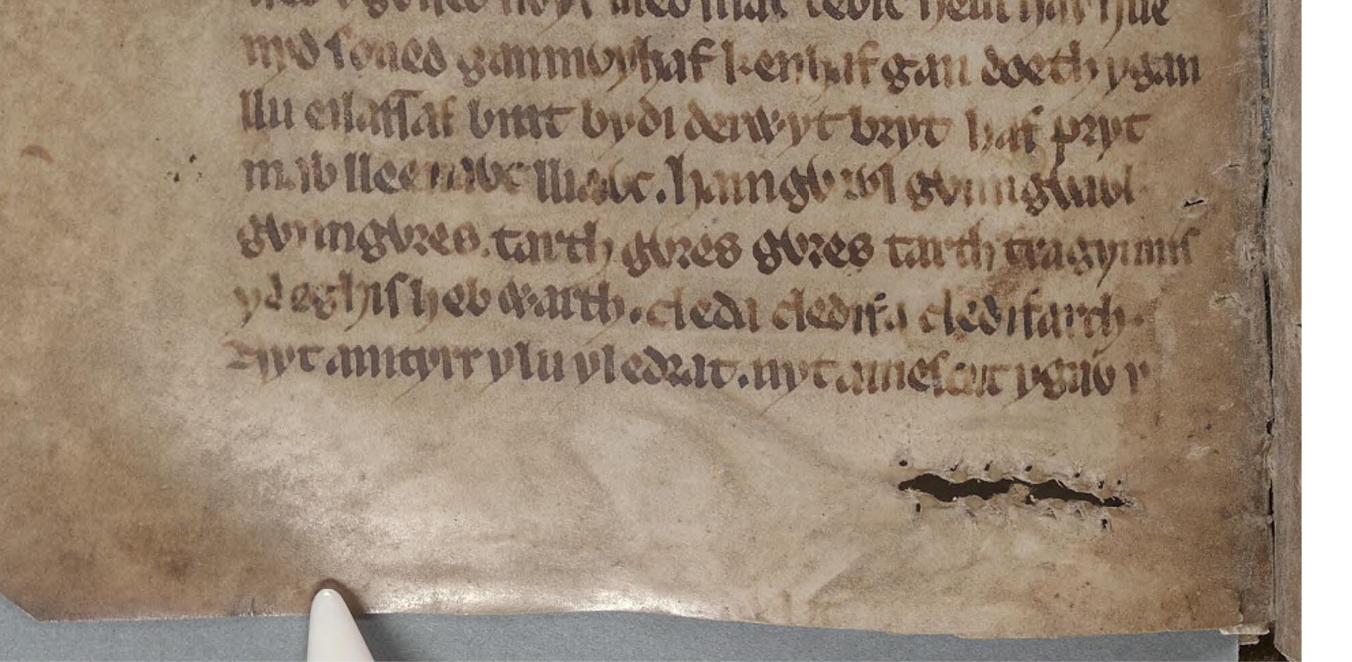
\includegraphics[width=\textwidth]{3orth/images/canvas.png}
    \caption[The bottom of \gls{bt} p.~64]{The bottom of \gls{bt} p.~64. Image credit: The National Library of Wales}
    \label{fig:p64}
\end{figure}

The easiest way to account for this situation is that scribe X86  copied the word \mw{kywlat} twice: first he wrote it as a catchword to make sure the quire starting with page 65 would be placed immediately following the quire ending with page 64. The second time it is found as the first word of page 65. In the first instance, he adds orthographic representation of lenition, and in the second he copies his exemplar directly. The reason he did not add lenition in the second instance is most likely due to him forgetting about the syntactic context of this word by the time he had his next quire before him. This instance singularly tells us that it was scribe X86 was the one who added orthographic lenition to his texts, and that his exemplar did not have lenition represented orthographically. 

\begin{mylongtable}{@{}lrrrlllll@{}}
\toprule
\textbf{IW} & \textbf{L.} & \textbf{P.\ MS} & \textbf{L.\ MS} & \textbf{Word} & \textbf{Translation} & \textbf{Cause of lenition} & \textbf{Represented} & \textbf{Initial C} \\ \midrule\endhead
II & 1 & 56 & 14 & \mw{gan} & `with' & petr & yes & c \\
II & 2 & 56 & 14 & \mw{wledic} & `lord' & \mw{am} & yes & g \\
II & 2 & 56 & 15 & \mw{gỽarthegyd} & `cowherd' & prep adj & no & g \\
II & 4 & 56 & 16 & \mw{teyrned} & `kingship' & obj len? & no & t \\
II & 7 & 56 & 19 & \mw{kyuygyd} & `warrior' & \mw{prep noun} & no & c \\
II & 9 & 56 & 20 & \mw{oꝛmes} & `oppression' & \mw{dy} & yes & g \\
II & 10 & 56 & 21 & \mw{dꝛos} & `over' & petr & yes & t \\
II & 11 & 56 & 21 & \mw{wyr} & `men' & obj len? & yes & g \\
II & 13 & 56 & 23 & \mw{tỽrỽf} & `clamour' & obj len? & no & t \\
II & 17 & 56 & 26 & \mw{wyr} & `men' & obj len? & yes & g \\
II & 19 & 57 & 1 & \mw{tanc} & `peace' & obj len? & no & t \\
II & 19 & 57 & 1 & \mw{gan} & `with' & petr & yes & c \\
II & 21 & 57 & 3 & \mw{gynrein} & `princes' & \mw{y} `his' & yes & c \\
II & 21 & 57 & 3 & \mw{kyỽym don} & `??' & ?? & no & c \\
II & 23 & 57 & 4 & \mw{wyr} & `men' & obj len? & yes & g \\
II & 24 & 57 & 5 & \mw{uaglei} & `snared' & \mw{a} & yes & m \\
II & 25 & 57 & 6 & \mw{kat} & `battle' & \mw{ỽrth} & no & c \\
II & 26 & 57 & 7 & \mw{pỽyllatt} & `knew' & \mw{pan} & no & p \\
II & 27 & 57 & 7 & \mw{ueidat} & `dared' & \mw{pan} & yes & b \\
II & 29 & 57 & 9 & \mw{alon} & `enemies' & \mw{e} `his' & yes & g \\
II & 29 & 57 & 9 & \mw{wen} & `white' & feminine noun & yes & g \\
II & 33 & 57 & 11 & \mw{vallỽyf} & `die' & \mw{yny} & yes & b \\
III & 6 & 57 & 16 & \mw{weſceryd} & `scatters' & \mw{yt} & yes & g \\
III & 8 & 57 & 16 & \mw{vo} & `may be' & \mw{tra} & yes & b \\
III & 8 & 57 & 16--17 & \mw{uuch/yd} & `life' & \mw{dy} & yes & b \\
III & 10 & 57 & 17 & \mw{gan} & `with' & petr & yes & c \\
III & 10 & 57 & 17 & \mw{clotuan} & `famous man' & \mw{gan} & no & c \\
III & 12 & 57 & 18 & \mw{vot} & `that … is' & ?? & yes & b \\
III & 12 & 57 & 18 & \mw{plant} & `children' & \mw{e} `his' & no & p \\
III & 14 & 57 & 19 & \mw{oꝛuchel} & `very high' & \mw{yn} & yes & g \\
III & 14 & 57 & 19 & \mw{wledic} & `lord' & prep adj & yes & g \\
III & 16 & 57 & 29 & \mw{keimyat} & `champion' & \mw{yn} & no & c \\
III & 19 & 57 & 21 & \mw{gaỽſſant} & `received' & \mw{a} & yes & c \\
III & 20 & 57 & 22 & \mw{godyant} & `rose' & parenthesis & yes & c \\
III & 23 & 57 & 23 & \mw{collet} & `lost' & prep adj & no & c \\
III & 25 & 57 & 23--24 & \mw{gaf/fel} & `have' & \mw{heb} & yes & c \\
III & 30 & 57 & 25 & \mw{pop} & `every' & \mw{o} & no & p \\
III & 31 & 57 & 26 & \mw{peleitrat} & `spear blow' & \mw{dy} & no & p \\
III & 32 & 57 & 26 & \mw{kat} & `battle' & verb ending? & no & c \\
III & 34 & 58 & 1 & \mw{wneit} & `you do' & \mw{a} & yes & g \\
III & 39 & 58 & 4 & \mw{waeſſaf} & `pledge' & \mw{heb} & yes & g \\
III & 40 & 58 & 4 & \mw{teyrn} & `ruler' & \mw{am} & no & t \\
III & 43 & 58 & 5 & \mw{uu} & `was' & \mw{a} & yes & b \\
III & 43 & 58 & 5 & \mw{uyd} & `will be' & \mw{a} & yes & b \\
III & 44 & 58 & 6 & \mw{kyſtedlyd} & `fellow' & \mw{oes} & no & c \\
III & 45 & 58 & 6 & \mw{dꝛemher} & `is seen' & \mw{pan} & yes & t \\
III & 48 & 58 & 8 & \mw{teyrn} & `ruler' & \mw{am} & no & t \\
III & 53 & 58 & 10 & \mw{vallỽyf} & `die' & \mw{yny} & yes & b \\
IV & 3 & 58 & 13 & \mw{parch} & `praise' & obj len? & no & p \\
IV & 6 & 58 & 15 & \mw{oꝛuoled} & `jubilation' & \mw{y} `to' & yes & g \\
IV & 7 & 58 & 15 & \mw{tired} & `lands' & prep adj & no & t \\
IV & 17 & 58 & 18 & \mw{lad} & `kills' & \mw{yt} & yes & ll \\
IV & 17 & 58 & 18 & \mw{gryc} & `hangs' & \mw{yt} & yes & c \\
IV & 18 & 58 & 19 & \mw{vac} & `cherishes' & \mw{yt} & yes & m \\
IV & 18 & 58 & 19 & \mw{vyc} & `honours' & \mw{yt} & yes & m \\
IV & 19 & 58 & 19 & \mw{vyc} & `honours' & \mw{yt} & yes & m \\
IV & 19 & 58 & 19 & \mw{vac} & `cherishes' & \mw{yt} & yes & m \\
IV & 20 & 58 & 19 & \mw{lad} & `kills' & \mw{yt} & yes & ll \\
IV & 22 & 58 & 20 & \mw{veird} & `bards' & \mw{y} `to' & yes & b \\
IV & 23 & 58 & 20 & \mw{geugant} & `certain' & \mw{yn } & yes & c \\
IV & 24 & 58 & 21 & \mw{wedant} & `they say' & \mw{yt} & yes & g \\
IV & 26 & 58 & 21--22 & \mw{pe/riſ} & `caused' & \mw{th} & no & p \\
IV & 35 & 58 & 25 & \mw{tỽrỽf} & `tumult' & prep adj & no & t \\
IV & 38 & 58 & 26 & \mw{trefret} & `homestead' & prep adj & no & t \\
IV & 39 & 58 & 26 & \mw{tudet} & `clothing' & prep adj & no & t \\
IV & 41 & 59 & 1 & \mw{van} & `bright' & epithet & yes & m \\
IV & 43 & 59 & 1 & \mw{trygan} & `sound' & \mw{un} & no & t \\
IV & 45 & 59 & 2 & \mw{gan} & `with' & epithet & yes & c \\
IV & 48 & 59 & 3 & \mw{gigleu} & `heard' & \mw{a} & yes & c \\
IV & 49 & 59 & 3 & \mw{ỽrdlideu} & `attributes' & \mw{y} `to' & yes & g \\
IV & 51 & 59 & 4 & \mw{weithredeu} & `works' & \mw{dy} & yes & g \\
IV & 52 & 59 & 4 & \mw{vallỽyf} & `die' & \mw{yny} & yes & b \\
V & 1 & 59 & 7 & \mw{blyned} & `years' & \mw{un} & no & b \\
V & 6 & 59 & 9 & \mw{vereu} & `spit' & \mw{am} & yes & b \\
V & 8 & 59 & 9--10 & \mw{gỽydua/eu} & `seats' & prep adj & no & c \\
V & 9 & 59 & 10 & \mw{wyt} & `food' & \mw{e} `his' & yes & b \\
V & 11 & 59 & 11 & \mw{varch} & `horse' & \mw{e} `his' & yes & m \\
V & 11 & 59 & 11 & \mw{danaỽ} & `under him' & petr & yes & t \\
V & 16 & 59 & 13 & \mw{loi} & `calves' & \mw{o} & yes & ll \\
V & 20 & 59 & 14 & \mw{lleas} & `death' & \mw{bei} & no & ll \\
V & 22 & 59 & 15 & \mw{kygryn} & `shivering' & feminine noun & no & c \\
V & 22 & 59 & 15 & \mw{kygryt} & `trembling' & feminine noun & no & c \\
V & 23 & 59 & 15 & \mw{wen} & `white' & feminine noun & yes & g \\
V & 23 & 59 & 15--16 & \mw{olch/et} & `washed' & feminine noun & yes & g \\
V & 26 & 59 & 26 & \mw{waet} & `blood' & \mw{am} & yes & g \\
V & 28 & 59 & 17 & \mw{uei} & `would be' & \mw{a} & yes & b \\
V & 28 & 59 & 17 & \mw{wedỽ} & `widow' & \mw{uei} & yes & g \\
V & 28 & 59 & 17 & \mw{wreic} & `wife' & \mw{y} `his' & yes & g \\
V & 30 & 59 & 18 & \mw{mynyc} & `frequent' & prep adj & no & m \\
V & 31 & 59 & 19 & \mw{poꝛth} & `gate' & \mw{am} & no & p \\
V & 31 & 59 & 19 & \mw{pen} & `head' & \mw{am} & no & p \\
V & 34 & 59 & 21 & \mw{trỽſt} & `noise' & \mw{py} & no & t \\
V & 35 & 59 & 21 & \mw{gryn} & `swells' & \mw{a} & yes & c \\
V & 38 & 59 & 22 & \mw{pedyt} & `infantry' & \mw{y} `his' & no & p \\
V & 44 & 59 & 25 & \mw{orꝛuyd} & `conquers' & \mw{a} & yes & g \\
V & 48 & 60 & 1 & \mw{blaỽd} & `strikes' & \mw{a} & yes & p \\
V & 54 & 60 & 3 & \mw{gylchyn} & `surroundings' & \mw{y} `his' & yes & c \\
V & 56 & 60 & 4 & \mw{par} & `spear' & \mw{y} `his' & no & p \\
V & 58 & 60 & 5 & \mw{vallỽyf} & `die' & \mw{yny} & yes & b \\
VI & 1 & 60 & 8 & \mw{uaỽr} & `big' & feminine noun & yes & m \\
VI & 1 & 60 & 8 & \mw{uu} & `was' & \mw{a} & yes & b \\
VI & 2 & 60 & 9 & \mw{gynnu} & `descends' & \mw{pan} & yes & c \\
VI & 7 & 60 & 12 & \mw{vaỽr} & `big' & epithet & yes & m \\
VI & 7 & 60 & 13 & \mw{trebyſtaỽt} & `commotion' & prep adj & no & t \\
VI & 8 & 60 & 13 & \mw{paraỽt} & `ready' & NP lenition & no & p \\
VI & 10 & 60 & 15 & \mw{paraỽt} & `ready' & NP lenition & no & p \\
VI & 11 & 60 & 15 & \mw{vab} & `son' & epithet & yes & m \\
VI & 11 & 60 & 16 & \mw{kymỽyaỽc} & `grieving' & \mw{-ei} & no & c \\
VI & 12 & 60 & 16 & \mw{leỽ} & `valiant' & prep adj & yes & g \\
VI & 12 & 60 & 16 & \mw{ỽyſtyl} & `bledge' & \mw{o} & yes & g \\
VI & 14 & 60 & 18 & \mw{gerenhyd} & `kindred' & \mw{am} & yes & c \\
VI & 17 & 60 & 20 & \mw{peleidyr} & `spears' & obj len? & no & p \\
VI & 18 & 60 & 21 & \mw{luyd} & `hosts' & \mw{y} `his' & yes & ll \\
VI & 19 & 60 & 21 & \mw{gyweithyd} & `company' & \mw{e} `his' & yes & c \\
VI & 22 & 60 & 23 & \mw{vꝛein} & `crows' & \mw{-ei} & yes & b \\
VI & 23 & 60 & 23 & \mw{gr\.{y}ſſỽys} & `charged' & \mw{a} & yes & c \\
VI & 23 & 60 & 24 & \mw{gan} & `with' & petr & yes & c \\
VI & 24 & 60 & 24 & \mw{blỽydyn} & `year' & obj len?/adv? & no & b \\
VI & 25 & 60 & 25 & \mw{vallỽyf} & `die' & \mw{yny} & yes & b \\
XI & 2 & 29 & 22 & \mw{biewyd} & `will have' & [\mw{a}] & yes & p \\
XI & 2 & 29 & 22 & \mw{gyneiluoaỽc} & `supporter' & \mw{obj len?} & yes & c \\
XI & 7 & 29 & 25 & \mw{bꝛydein} & (place name) & \mw{o} & yes & p \\
XI & 7 & 29 & 26 & \mw{gofein} & `memories' & \mw{prep noun} & yes & c \\
XI & 8 & 29 & 26 & \mw{berth} & `bush' & \mw{o} & yes & p \\
XI & 9 & 29--30 & 26--1 & \mw{ky/uerbyn} & `opposition' & \mw{obj len} & no & c \\
XI & 11 & 30 & 2 & \mw{lyghes} & `fleet' & \mw{y} `to' & yes & ll \\
XI & 12 & 30 & 2 & \mw{beleidyr} & `lances' & \mw{o} & yes & p \\
XI & 12 & 30 & 2 & \mw{bleigheit} & `battle' & \mw{o} & yes & p \\
XI & 12 & 30 & 2--3 & \mw{pꝛen/wres} & `??' & \mw{??} & ?? & ?? \\
XI & 13 & 30 & 3 & \mw{paỽb} & `everyone' & \mw{y} `to' & no & p \\
XI & 13 & 30 & 3 & \mw{trachwres} & `fury' & \mw{y} `his' & no & t \\
XI & 14 & 30 & 4 & \mw{gadeu} & `battles' & \mw{o} & yes & c \\
XI & 18 & 30 & 6 & \mw{vꝛetrỽyn} & (place name) & feminine noun & yes & b \\
XI & 18 & 30 & 7 & \mw{wres} & `heat' & \mw{trỽy} & yes & g \\
XI & 18 & 30 & 7 & \mw{tan} & `fire' & prep adj & no & t \\
XI & 19 & 30 & 7 & \mw{trachwres} & `fury' & \mw{y} `his' & no & t \\
XI & 23 & 30 & 10 & \mw{veibon} & `sons' & \mw{y} `to' & yes & m \\
XI & 25 & 30 & 11 & \mw{alon} & `enemies' & \mw{dy} & yes & g \\
XI & 27 & 30 & 11 & \mw{uraỽt} & `judgment' & \mw{ad} & yes & b \\
XI & 30 & 30 & 14 & \mw{gan} & `with' & petr & yes & c \\
XI & 30 & 30 & 14 & \mw{waỽꝛ} & `dawn' & \mw{gan} & yes & g \\
XI & 37 & 30 & 18 & \mw{wnaỽ} & `may do' & \mw{a} & yes & g \\
XI & 43 & 30 & 22 & \mw{gaenaỽc} & `armoured' & prep adj & yes & c \\
XI & 44 & 30 & 22 & \mw{wyl} & `sees' & \mw{ny} & yes & g \\
XI & 44 & 30 & 22 & \mw{welas} & `saw' & \mw{ny} & yes & g \\
XII & 1 & 63 & 25 & \mw{goꝛchoꝛdyon} & `hosts' & parenthesis & no & g \\
XII & 3 & 64 & 1 & \mw{gogyfres} & `united assault' & \mw{obj len} & no & g \\
XII & 5 & 64 & 2 & \mw{golychaf} & `I praise' & \mw{ny/[ry]} & no & g \\
XII & 5 & 64 & 2 & \mw{g(n)awd} & `praise' & \mw{a[r]} & no & g \\
XII & 5 & 64 & 2 & \mw{vꝛython} & (place name) & \mw{o} & yes & b \\
XII & 8 & 64 & 4 & \mw{wledic} & `ruler' & \mw{y} `to' & yes & g \\
XII & 9 & 64 & 5 & \mw{wlat} & `country' & fem art & yes & g \\
XII & 12 & 64 & 7 & \mw{wledic} & `ruler' & \mw{y} `to' & yes & g \\
XII & 12 & 64 & 7 & \mw{omed} & `refuses' & \mw{ni} & yes & g \\
XII & 14 & 64 & 8 & \mw{vyỽ} & `life' & \mw{y} `his' & yes & b \\
XII & 17 & 64 & 10 & \mw{pꝛeſſennaỽl} & `present' & fem noun & no & p \\
XII & 18 & 64 & 11 & \mw{gohoyỽ} & `fine' & \mw{ry} & no & g \\
XII & 18 & 64 & 11 & \mw{lyccraỽꝛ} & `is corrupted' & \mw{ry} & yes & ll \\
XII & 18 & 64 & 11 & \mw{lyccrer} & `must be corrupted' & \mw{ry} & yes & ll \\
XII & 19 & 64 & 12 & \mw{barnaỽꝛ} & `is judged' & \mw{ry} & no & b \\
XII & 20 & 64 & 12 & \mw{barn} & `judges' & \mw{ry} & no & b \\
XII & 22 & 64 & 13 & \mw{gỽr} & `man' & \mw{y} `to' & no & g \\
XII & 23 & 64 & 14 & \mw{traet} & `feet' & \mw{go} & no & t \\
XII & 25 & 64 & 15 & \mw{tebet} & `retreat' & \mw{ar} & no & t \\
XII & 26 & 64 & 16 & \mw{ofyn} & `ask' & \mw{ny} & yes & g \\
XII & 26 & 64 & 16 & \mw{wnech} & `may do' & \mw{a} & yes & g \\
XII & 30 & 64 & 18 & \mw{gynan} & (personal name) & parenthesis & yes & c \\
XII & 35 & 64 & 21 & \mw{gan} & `song' & prep noun & yes & c \\
XII & 36 & 64 & 21 & \mw{gan} & `with' & petr & yes & c \\
XII & 36 & 64 & 21 & \mw{gan} & `with' & petr & yes & c \\
XII & 36 & 64 & 22 & \mw{llu} & `host' & \mw{gan} & no & ll \\
XII & 37 & 64 & 22 & \mw{bydi} & `??' & NP lenition & yes & p \\
XII & 37 & 64 & 22 & \mw{bꝛyt} & `??' & \mw{??} & yes & p \\
XII & 38 & 64 & 23 & \mw{gỽaỽl} & (personal name) & \mw{ham} & no & g \\
XII & 39 & 64 & 24 & \mw{gỽres} & `heat' & obj len? & no & g \\
XII & 40 & 64 & 24 & \mw{gynniſ} & `kindled' & \mw{tra} & yes & c \\
XII & 42 & 64 & 26 & \mw{lu} & `host' & \mw{y} `his' & yes & ll \\
XII & 42 & 64 & 26 & \mw{ledꝛat} & `stealth' & \mw{y} `to' & yes & ll \\
XII & 43 & 64 & 26 & \mw{gaỽ} & `stop' & \mw{y} `to' & yes & c \\
XII & 43 & 64 & 27 & \mw{gywlat} & `enemy' & \mw{y} `his' & yes & c \\
XII & 44 & 65 & 1 & \mw{veirch} & `horses' & \mw{y} `his' & yes & m \\
XII & 45 & 65 & 2 & \mw{march} & `horse' & \mw{o} & no & m \\
XII & 46 & 65 & 2 & \mw{car} & `loves' & \mw{th} & no & c \\
XII & 48 & 65 & 3 & \mw{gaer} & (place name) & \mw{o} & yes & c \\
XII & 48 & 65 & 3 & \mw{glut} & (place name) & fem noun & yes & c \\
XII & 48 & 65 & 3--4 & \mw{ga/er} & (place name) & \mw{hyt} & yes & c \\
XII & 48 & 65 & 4 & \mw{garadaỽc} & (place name) & fem noun & yes & c \\
XII & 49 & 65 & 4 & \mw{gỽallaỽc} & (personal name) & \mw{a} & no & g \\ \bottomrule
\caption{CT}
\label{my-label}
\end{mylongtable}

\subsection{Armes Prydein Vawr}
The poem \mw{Armes Prydein Vawr} `the Great Prophecy of Britain' is also found in the \gls{bt} on pages 13--18. It is independently dateable on the basis of the political elements found in it. Ifor Williams argues that the poem was composed before the Norman conquest of 1066, because it prophecies deliverance from the Saxons, and there is no point in making such a prophecy when the result of this would be that the Normans would still be in power. Furthermore, the poem differentiates between men of Dublin and Irishmen of Ireland, meaning the poem postdates the settlement of the Vikings in the ninth century. In addition, the name \mw{Glywysing} is used for an area roughly coterminous with Glamorgan, which Williams considers an archaism. Ifor Williams dates the composition of this poem to about 900 on the basis of these considerations~\autocite[x--xii]{williams_armes_1955}. \Textcite{dumville_brittany_1983} dates the poem to a date later in the tenth century. 


\begin{table}[h]
\centering
\begin{tabular}{@{}rlll@{}}
\toprule
 & \textbf{Rep.} & \textbf{Not rep.} & \textbf{Total} \\ \midrule
T & 62 & 25 & 87 \\
Not T & 55 & 8 & 63 \\
\textbf{Total} & \textbf{117} & \textbf{33} & \textbf{150} \\ \bottomrule
\end{tabular}
\caption{Correspondence between initial consonant type and orthographic representation of lenition in \mw{Armes Prydein Vawr}.}
\label{armesprydeinnumbers}
\end{table}

% Table \ref{armesprydeinnumbers} shows that there is a correlation between consonant type and lenition. The two-tailed P value according to Fisher's exact test equals $0.0272<0.05$. This shows that the null hypothesis (the initial consonant being a voiceless stop or another consonant has no bearing upon orthographic representation of lenition) must be rejected.

It is the distribution, not the raw frequency of non-orthographical representation that tells us about the date of an exemplar. Nevertheless, only a minority of about two-fifths of the voiceless stops are not lenited. This number agrees with the other prophecies.

\subsubsection{Hypercorrect insertion of lenition}
In several cases, lenition is written where I have no explanation for it. They are found in the following lines (translations taken from \textcite{williams_armes_1972}):

\begin{mwl}
\mwc[gwssyl]{\mw{Armes Prydein} l.~108 (\gls{bt} 16.7)}{pan dyffo iwyſ y vn gỽſſyl}{when the men of Wessex will come together in council,}
\mwc[gyghor]{\mw{Armes Prydein} l.~109 (\gls{bt} 16.7--8}{Vn coꝛ vn gyg/hoꝛ a lloegyr lloscit}{in a single party, of one mind with the Mercian incendiaries,}
\end{mwl}

Both examples contain a lenited masculine noun after \mw{vn} `one'. 
Example~\ref{gwssyl} has \mw[council]{gỽſſyl}, and  Example~\ref{gyghor} has \mw[council]{gyghoꝛ}. 
Two words that mean roughly the same are erroneously lenited under the same circumstances, and they are on the same line in the manuscript. In the second case, (non-represented) lenition of \mw{coꝛ} `party' may have influenced the decision to write lenition here\footnote{\mw{coꝛ} `party' is itself problematic here. \Textcite[s.v.\ côr\textsuperscript{1}]{bevan_geiriadur_2014} shows that this word may be both masculine and feminine, but l~48 \mw{goꝛ}	`meeting' may imply that it was feminine at least in this instance.}. Another possible solution is that \mw{un} means not `one', but `same' in both problematic instances. If this is the case, then lenition is justified, as \mw{un} meaning `same' may be considered a preposed adjective. Even if this is not what the author of the original composition meant to say, it is possible that the scribe of the \gls{bt} understood \mw{un} as such here, and lenited accordingly.



\subsubsection{Non-representation of lenition of ¬\acrshort{T}}
Among the non-voiceless stops whose lenition is not represented orthographically, all cases except one have an initial \mw{g}. Perhaps this is a relic from the \gls{ow} practice to represent /\cw/ with \mw{gu}. Etymologically, each of these cases except one has a /\cw/ following the /g/: l.~8	\mw{goꝛuoled},
l.~58	\mw{Gỽy},
l.~123	\mw{gỽerth},
l.~143	\mw{gỽerth},
l.~151	\mw{gỽyr}, and
l.~167	\mw{gỽlatwarthegyd}, while
l.~176	\mw{gynhon} starts with an etymological /g/. 

The one remaining case is l.~80	\mw{mỽyn} `benefit', which should be lenited due to parenthesis in the following line: 
\mwcc[mwyn]{\mw{Armes Prydein} l.~80 (\gls{bt} 15.11--12)}{ny byd y vedyc mỽyn oꝛ a wnaant.}{The doctor will not have benefit from what they do.}
Here, \mw[benefit]{mỽyn} follows the noun \mw[doctor]{vedyc} and may therefore have been misinterpreted by the scribe as adjective \mw[mild, tender]{mwyn}. 
Regardless of the validity of this explanation, this assumes that lenition of a non-voiceless stop was not represented in an original composition either. 
This means that this word presents a singular counterexample to the argument that \mw{Armes Prydein} stems from a period when lenition was written, but not lenition of voiceless stops.



\begin{mylongtable}{@{}rlllll@{}}
\toprule
\textbf{Line} & \textbf{Word} & \textbf{Translation} & \textbf{Cause of lenition} & \textbf{Represented} \\ \midrule\endhead
2 & \mw{genhyn} & `with them' & petrified lenition & yes \\
7 & \mw{Gaer} & `Fort' & \mw{hyt} & yes \\
7 & \mw{Weir} & (place name) & feminine noun & yes \\
8 & \mw{goꝛuoled} & `jubilation' & object lenition & no \\
11 & \mw{genhyn} & `with them' & petrified lenition & yes \\
12 & \mw{uyd} & `will be' & [\mw{a}] & yes \\
19 & \mw{gỽynyn} & `they complain' & \mw{a} & yes \\
22 & \mw{telhyn} & `they pay' & \mw{a} & no \\
23 & \mw{ỽr} & `man' & NP lenition & yes \\
24 & \mw{talei} & `will pay' & \mw{a} & no \\
25 & \mw{eir} & `word' & \mw{a} `from' & yes \\
30 & \mw{wydynt} & `they know' & \mw{ny} & yes \\
30 & \mw{treiglynt} & `they pass' & \mw{py} & no \\
31 & \mw{pꝛynaſſant} & `they bought' & \mw{pan} & no \\
31 & \mw{Danet} & (place name) & object lenition & yes \\
32 & \mw{gan} & `by' & petrified lenition & yes \\
35 & \mw{wiraỽt} & `liquor' & preposed adjective & yes \\
35 & \mw{ved} & `mead' & \mw{o} & yes \\
40 & \mw{uyd} & `will be' & \mw{pan} & yes \\
41 & \mw{bỽyller} & `is intended' & \mw{a} & yes \\
42 & \mw{Vꝛython} & `Britons' & feminine noun & yes \\
45 & \mw{eir} & `word' & \mw{a} `from' & yes \\
48 & \mw{goꝛ} & `meeting' & \mw{un} & yes \\
48 & \mw{gyghoꝛ} & `council' & \mw{un} & yes \\
55 & \mw{lan} & `edge' & \mw{am} & yes \\
56 & \mw{vydinaỽr} & `armies' & preposed adjective & yes \\
58 & \mw{Gỽy} & (place name) & \mw{am} & no \\
58 & \mw{peurllyn} & `bright lake' & \mw{am} & no \\
61 & \mw{kynyrcheit} & `gathering' & preposed genitive & no \\
62 & \mw{von} & `stem' & \mw{ỽrth} & yes \\
65 & \mw{goet} & `wood' & \mw{trỽy} & yes \\
66 & \mw{uỽꝛch} & `wall' & \mw{trỽy} & yes \\
67 & \mw{tir} & `land' & \mw{y} `to' & no \\
68 & \mw{laỽ} & `hand' & \mw{trỽy} & yes \\
68 & \mw{gyghoꝛ} & `council' & feminine noun & yes \\
69 & \mw{Geri} & (place name) & feminine noun & yes \\
74 & \mw{watwar} & `taunting' & preposed adjective & yes \\
76 & \mw{oꝛolchant} & `drench' & \mw{a} & yes \\
77 & \mw{kyneircheit} & `courtiers' & preposed genitive & no \\
80 & \mw{vedyc} & `doctor' & \mw{y} `to' & yes \\
80 & \mw{mỽyn} & `benefit' & parenthesis & no \\
80 & \mw{wnaant} & `they do' & \mw{a} & yes \\
82 & \mw{wnant} & `they do' & \mw{a} & yes \\
84 & \mw{ỽdant} & `they know' & \mw{a} & yes \\
88 & \mw{gerd} & `goes' & \mw{a} & yes \\
88 & \mw{genhyn} & `with them' & petrified lenition & yes \\
91 & \mw{baladyr} & `lance' & \mw{yn} & yes \\
91 & \mw{gan} & `with' & petrified lenition & yes \\
93 & \mw{dꝛoſ} & `over' & petrified lenition & yes \\
94 & \mw{rud} & `cheek' & \mw{ar} & yes \\
96 & \mw{Gaer} & `Fort' & \mw{hyt} & yes \\
96 & \mw{Wynt} & (place name) & feminine noun & yes \\
97 & \mw{Gymry} & `Welshmen' & epithet & yes \\
98 & \mw{trindaỽt} & `trinity' & feminine article & no \\
98 & \mw{gynt} & `former' & adverbial phrase & yes \\
102 & \mw{genhyn} & `with them' & petrified lenition & yes \\
103 & \mw{talet} & `payment' & \mw{heb} & no \\
103 & \mw{dynget} & `fate' & \mw{o} & yes \\
103 & \mw{geffyn} & `we have' & \mw{a} & yes \\
104 & \mw{veibon} & `sons' & preposed adjective & yes \\
108 & \mw{gỽſſyl} & `council' & ?? & yes \\
109 & \mw{gyghoꝛ} & `council' & ?? & yes \\
110 & \mw{luyd} & `host' & preposed adjective & yes \\
111 & \mw{beunyd} & `every day' & adverbial phrase & yes \\
112 & \mw{ỽyr} & `knows' & \mw{ny} & yes \\
112 & \mw{uyd} & `will be' & [\mw{a}] & yes \\
113 & \mw{gyfarth} & `barking' & object lenition & yes \\
113 & \mw{vynyd} & `mountain' & \mw{o} & yes \\
114 & \mw{talu} & `pay' & \mw{\.{y}} `to' & no \\
116 & \mw{coꝛff} & `body' & object lenition & no \\
116 & \mw{gilyd} & `companion' & \mw{y} `his' & yes \\
122 & \mw{galaned} & `corpses' & subject of plural verb & yes \\
123 & \mw{treth} & `tax' & feminine article & no \\
123 & \mw{gỽerth} & `value' & \mw{ar} & no \\
123 & \mw{beunyd} & `every day' & adverbial phrase & yes \\
124 & \mw{gennadeu} & `messengers' & preposed adjective & yes \\
124 & \mw{luyd} & `host' & preposed adjective & yes \\
125 & \mw{kyfergyr} & `conflict' & \mw{trỽy} & no \\
126 & \mw{gyweir} & `ordered' & \mw{yn} & yes \\
126 & \mw{gyteir} & `unanimous' & adverbial phrase & yes \\
126 & \mw{g\.{y}tſon} & `harmonious' & adverbial phrase & yes \\
126 & \mw{gytffyd} & `of one faith' & adverbial phrase & yes \\
127 & \mw{peri} & `cause' & \mw{y} `to' & no \\
128 & \mw{gynnullant} & `they assemble' & \mw{a} & yes \\
130 & \mw{tywyſſaỽ} & `lead' & \mw{y} `to' & no \\
130 & \mw{lieingant} & `circle of linen' & \mw{trỽy} & yes \\
131 & \mw{genhyn} & `with them' & petrified lenition & yes \\
132 & \mw{gat} & `battle' & feminine article & yes \\
133 & \mw{geiſſyſſant} & `they seek' & [\mw{a}] & yes \\
134 & \mw{wlad} & `country' & feminine article & yes \\
136 & \mw{vꝛo} & `land' & \mw{py} & yes \\
137 & \mw{genhyn} & `with them' & petrified lenition & yes \\
138 & \mw{wir} & `true' & \mw{o} & yes \\
139 & \mw{vꝛeint} & `privilage' & \mw{Neu} & yes \\
141 & \mw{Gymry} & `Welshmen' & subject of plural verb & yes \\
143 & \mw{talhont} & `they pay' & \mw{pan} & no \\
143 & \mw{gỽerth} & `worth' & preposed adjective & no \\
145 & \mw{garant} & `they love' & [\mw{a}] & yes \\
149 & \mw{lygheſ} & `fleet' & parenthesis & yes \\
150 & \mw{gat} & `battle' & feminine article & yes \\
151 & \mw{gỽyr} & `men' & parenthesis & no \\
152 & \mw{Pꝛydein} & `Britain' & \mw{o} & no \\
152 & \mw{virein} & `fair' & parenthesis & yes \\
152 & \mw{luyd} & `host' & preposed adjective & yes \\
153 & \mw{Lydaỽ} & `Brittany' & \mw{o} & yes \\
153 & \mw{pꝛydaỽ} & `lovely' & parenthesis & no \\
153 & \mw{gywiethyd} & `company' & preposed adjective & yes \\
154 & \mw{katueirch} & `warhorse' & \mw{ar} & no \\
155 & \mw{pop} & `every' & \mw{o} & no \\
157 & \mw{gyweithyd} & `company' & preposed adjective & yes \\
164 & \mw{vꝛaỽt} & `judgment' & \mw{hyt} & yes \\
166 & \mw{oꝛſegyn} & `trampler' & \mw{deu} & yes \\
166 & \mw{pleit} & `side' & \mw{o} & no \\
167 & \mw{gedaỽl} & `generous' & \mw{deu} & yes \\
167 & \mw{gỽlatwarthegyd} & `land-cowman' & preposed adjective & no \\
168 & \mw{baraỽt} & `ready' & preposed adjective & yes \\
169 & \mw{luyd} & `host' & preposed adjective & yes \\
170 & \mw{beunyd} & `every day' & adverbial phrase & yes \\
172 & \mw{Vynaỽ} & `Isle of Man' & \mw{o} & yes \\
172 & \mw{Lydaỽ} & `Brittany' & \mw{hyt} & yes \\
172 & \mw{vyd} & `will be' & \mw{yt} & yes \\
173 & \mw{Danet} & (place name) & \mw{hyt} & yes \\
173 & \mw{bieiuyd} & `will posess' & [\mw{a}] & yes \\
174 & \mw{Waỽl} & (place name) & \mw{o} & yes \\
174 & \mw{Weryt} & (place name) & \mw{hyt} & yes \\
176 & \mw{gynhon} & `tribes' & \mw{ar} & no \\
177 & \mw{Ỽydyl} & `Irishmen' & subject of plural verb & yes \\
178 & \mw{Gymry} & `Welshmen' & subject of plural verb & yes \\
178 & \mw{kadyr} & `powerful' & object lenition & no \\
178 & \mw{gyweithyd} & `company' & preposed adjective & yes \\
179 & \mw{gỽꝛỽf} & `ale' & \mw{am} & yes \\
180 & \mw{gedỽyſ} & `kept' & \mw{ry} & yes \\
181 & \mw{pop} & `every' & \mw{y} `to' & no \\
182 & \mw{gan} & `with' & petrified lenition & yes \\
182 & \mw{gilyd} & `companion' & \mw{y} `his' & yes \\
183 & \mw{alwaỽꝛ} & `call' & \mw{ny} & yes \\
183 & \mw{gynifwyr} & `warrior' & \mw{yn} & yes \\
184 & \mw{gyfnewitwyr} & `merchants' & \mw{e} `his' & yes \\
185 & \mw{uyd} & `will be' & [\mw{a}] & yes \\
186 & \mw{gymỽyeit} & `warriors' & feminine noun & yes \\
187 & \mw{galaned} & `corpses' & subject of plural verb & yes \\
188 & \mw{vyd} & `will be' & [\mw{a}] & yes \\
189 & \mw{gychwyn} & `start' & \mw{ar} & yes \\
191 & \mw{voꝛ} & `sea' & \mw{ar} & yes \\
191 & \mw{peunyd} & `every day' & petrified lenition & no \\
192 & \mw{vꝛaỽt} & `judgment' & \mw{hyt} & yes \\
193 & \mw{lyfraỽꝛ} & `books' & object lenition & yes \\
193 & \mw{bꝛydyd} & `poet' & preposed adjective & yes \\
195 & \mw{greỽys} & `created' & \mw{a} & yes \\
197 & \mw{Kaer} & `fort' & feminine noun & no \\
199 & \mw{ỽyỽ} & `withered' & \mw{ny} & yes \\
199 & \mw{wellyc} & `neglected' & \mw{ny} & yes \\ \bottomrule
\caption{Representation of lenition in \mw{Armes Prydein}}
\label{armesprydein}
\end{mylongtable}


\subsection{Prophecies}
Here, I discuss several prophecies together in one section. I discuss these together because they are similar linguistically and in terms of content, and usually not long enough to make reliable inferences about them individually. I have analysed eight out of ten poems edited in `Prophecies from the Book of Taliesin' by \textcite{haycock_prophecies_2013}. I have not included \mw{Gwawt Lud y mawr} and \mw{Yn wir dymbi Romani kar}, because they are not easily dateable. Other poems are datable, and Haycock dates them with varying degrees of certainty to the tenth to the thirteenth century, as shown in Table \ref{proprep}. 
\begin{table}[h]
\centering
\begin{tabular}{@{}llddddl@{}}
  \toprule
  \tch{Text} & \tch{Table} & \tchh{T} & \tchh{Not T} & \tch{Date}\\
                              &  & \tch{rep.} & \tch{not rep.} & \tch{rep.} & \tch{not rep.} \\ \midrule
  \mw{Daronwy} & \ref{prop1} & 5 & 13 & 21 & 0  & 13c \\
  \mw{Glaswawt Taliessin} & \ref{prop2} & 9 & 3 & 11 & 0 & 10--13c\\
  \mw{Kychwedyl a’m dodyw…} & \ref{prop3} & 19 & 5 & 28 & 4 & 13c\\
  \mw{Dygogan awen} & \ref{prop4} & 2 & 3 & 11 & 1 & ll.\ 1--4: 10c\\
  \mw{Kein gyfedwch} & \ref{prop5} & 7 & 3 & 10 & 0 & 13c\\
  \mw{Rydyrchafwy Duw…} & \ref{prop6} & 6 & 5 & 15 & 1 & 10--13c\\
  \mw{Ymarwar Llud bychan} & \ref{prop9} & 1 & 4 & 5 & 1 & 10c\\
  \mw{Darogan Kadwal[adyr]} & \ref{prop10} & 5 & 2 & 3 & 0 & pre-Norman\\
  {Total} &  & {54} & {38} & {104} & {7} & \\ \bottomrule
\end{tabular}
\caption{Representation of lenition in the prophetic texts and their dates of composition according to \textcite[\emph{passim}]{haycock_prophecies_2013}.}
\label{proprep}
\end{table}

Table~\ref{proprep} shows that lenition of voiceless stops was not represented in about forty~per cent of cases. For other consonants, non-representation of lenition is confined to a handful of instances, which are best discussed individually.

Haycock's poems dated to the tenth until the thirteenth century have little positive evidence pointing towards a date in the later end of the spectrum. Typically, these poems have historical references pointing to the tenth century, but a date up to the thirteenth-century may not be excluded as long as there is no evidence to do so. Nevertheless, I will assume for the purpose of this chapter that these poems were written when they were most relevant, edging closer to a starting date. 

\subsubsection{Non-representation of lenition of ¬T}
Two out of seven non-represented lenited non-voiceless stops were expected to cause object lenition. Table~\ref{propobjlen} shows all instances where object lenition may be represented, but it is only represented twice. Both voiceless stops and other consonants are often left unlenited. \Textcite[72--73]{van_development14} shows that verbal endings causing object lenition initially did not cause object lenition. Rather, it has developed over the course of the \gls{mw} period. Before the thirteenth century, object lenition was not typically written, although object lenition may sometimes leak through in exemplars from the thirteenth century onward. I assume that the same is the case here: although the scribe of the \gls{bt} may have had object lenition as part of his Welsh grammar, the exemplars he copied most likely predated object lenition, and were thus inconsistently modernised in a manner similar to how the representation of lenited voiceless stops came to be modernised irregularly.

\begin{table}[h]
\centering
\begin{tabular}{@{}lllll@{}}
\toprule
\textbf{Poem} & \textbf{Line} & \textbf{Word} & \textbf{Translation} & \textbf{rep.} \\ \midrule
\mw{Daronwy} & 44 & \mw{kamualhau} & `hide' & no \\
\mw{Kychwedyl a’m dodyw…} & 13 & \mw{trỽy/det} & `passage' & no \\
\mw{Kychwedyl a’m dodyw…} & 18 & \mw{biỽ} & `cattle' & no \\
\mw{Dygogan awen} & 25 & \mw{kyfamrud} & `bloodshed' & no \\
\mw{Rydyrchafwy Duw…} & 10 & \mw{wyr} & `men' & yes \\
\mw{Ymarwar Llud bychan} & 3 & \mw{Pꝛydein} & (place name) & no \\
\mw{Ymarwar Llud bychan} & 18 & \mw{mab} & `son' & no \\
\mw{Darogan Kadwal[adyr]} & 15 & \mw{gelein} & `corpse' & yes \\ \bottomrule
\end{tabular}
\caption{Representation of object lenition in the Prophecies from the \gls{bt}}
\label{propobjlen}
\end{table}

A few instances of non-representation of lenition are found in Example~\ref{gwyargorgolchei}. 
\mwcc[gwyargorgolchei]{\mw{Kychwedyl} l.\ 53 (\gls{bt} 39.20--21)}{gỽyar goꝛgol/che[i] gỽarthaf iat.}{blood washed over the top of the head(s).}
Here, we would expect \mw{goꝛgolchei} `washed over' to be lenited, because it follows its subject and therefore is preceded by verbal particle \mw{a}, which may or may not be written out in full, but always causes lenition. Additionally, the ending in \ei\ consistently causes lenition throughout the \gls{mw} period, and therefore \mw{gỽarthafiat} `heads' should be lenited~\Autocite[42--45]{van_development14}. Note also that the second \mw{g} in \mw{goꝛgolchei} also represents a lenited /g/, and is another case in which lenition is not represented. Although representation of word-medial lenition is not under investigation here, it is striking that three \mw{g}'s are all kept. 

I hypothesise that the key lies in the cynghanedd. By not representing lenition, all these unlenited \mw{g}'s still looked like they alliterated with the first word \mw{gỽyar} `blood'. When the poem was written, lenited and unlenited consonants most likely still could alliterate. When it was copied into the \gls{bt}, they could not. The scribe subsequently had to make a choice between breaking the alliteration pattern or breaking rules of lenition, and apparently chose the latter option.

This leaves the following three instances failing to write lenition of a consonant other than a voiceless stop:
\begin{mwl}
\mwc[gwehenyt]{\mw{Kychwedyl} l.\ 30 (\gls{bt} 39.5--6)}{Gỽlat vabon gỽehenyt anoleithat}{(came) the inescapable destroyer from the land of Mabon}
\mwc[gynhon]{\mw{Dygogan awen} l.\ 26 (\gls{bt} 71.4--5)}{a chat y gynhon}{and battle for the foreigners}
\mwc[gwnant]{\mw{Rydyrchafwy Duw…} l.\ 12 (\gls{bt} 73.5--6)}{ỽy gwnant aer ar vꝛys amlys lonyon.}{they shall make battle in haste around the court of Llonion.}
\end{mwl}
In Example~\ref{gwehenyt}, \mw{gỽehenyt} `destroyer' should be lenited because it follows a preposed genitive, but it is not. Perhaps alliteration with \mw{Gỽlat} `land' was deemed more important than grammatical correctness here. Example~\ref{gynhon} has unlenited \mw{gynhon} following \mw{y} `to'. Perhaps this was due to the scribe misunderstanding \mw{y} to be the article here, or any other \mw{y} that does not cause lenition. Example~\ref{gwnant} is not lenited, although it follows its subject and therefore is preceded by verbal particle \mw{a}, which may or may not be written out in full, but always causes lenition. I have no explanation for this example other than that absence of the verbal particle would make it easy for a scribe to make a mistake in modernising lenition here.

Nevertheless, the general dearth of failure to lenite consonants other than voiceless stops suggests that we are dealing with a scribe who worked on exemplars that already showed lenition, but not of voiceless stops, and subsequently inserted lenition in about sixty per cent of cases where it would be appropriate. An alternative explanation would be that all lenition would be inserted by this scribe, and that the scribe had a sixty-percent success rate in modernising lenition of voiceless stops, and a near-hundred-percent success rate in modernising other types of consonants. The former explanation seems preferable to me\todo{The 60\% figure roughly agrees with CA}.

\subsubsection{Hypercorrect insertion of lenition}
On several occasions, lenition is written with no obvious grammatical cause. I list them below, followed by an account of how lenition may have come to be inserted. Translations are by \textcite[\emph{passim}]{haycock_prophecies_2013}.


\begin{mwl}
\mwc[ofrwy]{\mw{Daronwy} l.~2 (\gls{bt} 28.22)}{rac llanỽ llet ofrỽy}{from the Flood, a radiant extent}
\mwc[barawt]{\mw{Glaswawt Taliessin} l.~9 (\gls{bt} 31.5)}{Adoer lleith dyrreith anaỽ baraỽt}{Chilling the death which came about --- ready reward ---}
\mwc[droch]{\mw{Glaswawt Taliessin} l.~11 (\gls{bt} 31.6--7)}{Tꝛi dillyn diachoꝛ dꝛoch dꝛymluaỽc.}{Three trim invincible ones, heavily-laden in the water with hosts,}
\mwc[lawen]{\mw{Kychwedyl a’m dodyw…} l.~4 (\gls{bt} 38.13--14)}{Ỻaỽn yỽ y yſtrat lawen gynnyd.}{his valley-floor is full --- a joyous gain,}
\mwc[ochwynogyon]{\mw{Kychwedyl a’m dodyw…} l.~41 (\gls{bt} 39.12--13)}{Nyth y ogyfeirch ochwynogyon}{no complainants (need to) importune you.}
\mwc[virein]{\mw{Kein gyfedwch} l.~3 (\gls{bt} 72.11)}{virein ffo racdaỽ. ar lleg kaỽ mỽyedic uein.}{a wondrous retreat before him --- the one who has a well-wrought protection of reinforced stones.}
\mwc[eir]{\mw{Rydyrchafwy Duw…} l.~8 (\gls{bt} 73.2)}{yn un redyf vn eir kywir kymon.}{with one instinct, one utterance, orderly and disciplined,}
\end{mwl}
In Example~\ref{ofrwy}, \mw{ofrỽy} `fine, radiant' is lenited. It is an adjective following masculine noun \mw{llet} `extent'. 
Similarly, Example~\ref{barawt} has lenited \mw{baraỽt} `ready' following masculine \mw{anaỽ} `reward'. 
Example~\ref{droch} has two instances of lenition defying easy explanation. Lenited \mw{dꝛoch} `immersion' is the first, and has no syntactic connection with the previous word.  The following word \mw{dꝛymluaỽc} `loaded' is the second word which is puzzlingly lenited.  The scribe may have inserted lenition twice here in order to maintain alliteration between these two words, in a manner similarly to how lenition was not added in Example~\ref{gwehenyt}. However, this leaves the question why either would lenite in the first place unsolved. 
In Example~\ref{lawen}, \mw{lawen}	`joyous' has no reason to be lenited. This is all the more puzzling because it alliterates with \mw{Ỻaỽn} `full' in the first half of the line. A possible solution lies in the fact that the previous word, \mw{yſtrat} `valley-floor', is feminine, and the scribe thought \mw{lawen} was connected to it. 
Example~\ref{ochwynogyon} has \mw{ochwynogyon}	`complainants', a subject following a third-person present indicative verb, which is  thus not a candidate for either postverbal lenition or object lenition. Perhaps, however, the scribe misread this word as the object of the sentence, and inserted object lenition accordingly. 
In Example~\ref{virein}, \mw{virein} `wondrous' is lenited, even though it is the first word of its line and thus nothing preceding could lenite it. However, the previous line ends with a verb, and the scribe may have thought these words to be connected, and lenited accordingly. 
Example~\ref{eir} has lenited \mw{eir}	`utterance', a masculine noun, following \mw{un} `one'. This one may be lenited analogously with the feminine noun in \mw{un redyf} `one instinct', in order to maintain alliteration. An alternative explanation is similar to the one given with Examples~\ref{gwssyl} and \ref{gyghor}, meaning \mw{un} may be translated with `same', and always cause lenition.

Examples of lenition where we would not expect it are rare, but nevertheless imply that the scribe added lenition where there was none in an earlier written version of the same text. What do we make of this? On the one hand, this supports my argument that lenition of voiceless stops was added at a later date in the \gls{bt}, because mistakes and hypercorrections always  exist where orthography is updated. On the other hand, the hypercorrect additions of lenition are  also of other consonants. One complicating factor is that it seems the prophecies were written in a period when lenited and unlenited consonants could alliterate, but that the representation of lenition was updated at a point when they could no longer do so. This gave the scribe updating representation of lenition a double job: he had to modernise lenition in such a way that it agreed with the grammatical conditions for lenition, but he also had to modernise it in such a way as to respect the alliteration patterns. 



\begin{table}[H]
\centering
\begin{tabular}{@{}lllll@{}}
\toprule
\textbf{Line} & \textbf{Word} & \textbf{Translation} & \textbf{Cause of len.} & \textbf{rep.} \\ \midrule
2 & \mw{ofrỽy} & `fine' & ?? & yes \\
3 & \mw{tarrỽy} & `spreads out' & \mw{a} & no \\
4 & \mw{treiſ} & `attacks' & \mw{a} & no \\
4 & \mw{dꝛoſ} & `over' & petrified & yes \\
4 & \mw{voꝛdỽy} & `surging sea' & \mw{dꝛoſ} & yes \\
5 & \mw{prꝛen} & `tree' & \mw{py} & no \\
5 & \mw{vo} & `may be' & \mw{a} & yes \\
9 & \mw{uỽy} & `more' & NP lenition & yes \\
12 & \mw{Vathonỽy} & (personal name) & feminine noun & yes \\
13 & \mw{tyfỽy} & `grows' & \mw{pan} & no \\
15 & \mw{lan} & `bank' & \mw{ar} & yes \\
17 & \mw{wledych/ỽy} & `rules' & \mw{pan} & yes \\
19 & \mw{trei} & `ebb' & \mw{troſ} & no \\
19 & \mw{traeth} & `shore' & \mw{throſ} & no \\
20 & \mw{pennaeth} & `dominion' & preposed adj. & no \\
21 & \mw{pymhet} & `fifth' & feminine article & no \\
23 & \mw{Pꝛydein} & (place name) & \mw{ar} & no \\
24 & \mw{ui} & `will be' & \mw{a} & yes \\
25 & \mw{ui} & `will be' & \mw{a} & yes \\
29 & \mw{vein} & `slender' & preposed adj. & yes \\
31 & \mw{wyr} & `men' & \mw{ar} & yes \\
34 & \mw{gyg/ein} & `fits' & \mw{a} & yes \\
37 & \mw{gerd} & `song' & \mw{ar} & yes \\
37 & \mw{gygein} & `fits' & \mw{yt} & yes \\
38 & \mw{tynnu} & `sniff' & \mw{y} `to' & no \\
39 & \mw{wan} & `gore' & \mw{y} `to' & yes \\
39 & \mw{tyruu} & `root' & \mw{y} `to' & no \\
40 & \mw{w/naeth} & `made' & \mw{a} & yes \\
41 & \mw{wiſc} & `line' & \mw{o} & yes \\
43 & \mw{uuant} & `they were' & \mw{yt} & yes \\
43 & \mw{uu} & `was' & \mw{yt} & yes \\
44 & \mw{wnel} & `do' & \mw{pan} & yes \\
44 & \mw{kamualhau} & `hide' & object lenition & no \\
46 & \mw{lam} & `leap' & \mw{i} `to' & yes \\
46 & \mw{lam} & `leap' & \mw{o} & yes \\
47 & \mw{keỽſſit} & `had' & [\mw{a}] & no \\
47 & \mw{gaho} & `has' & \mw{nyr} & yes \\
48 & \mw{ỽc} & `threatens' & \mw{a} & yes \\
51 & \mw{wyl} & `sees' & \mw{a} & yes \\ \bottomrule
\end{tabular}
\caption{Representation of lenition in \mw{Daronwy}}
\label{prop1}
\end{table}



\begin{table}[h]
\centering
\begin{tabular}{@{}lllll@{}}
\toprule
\textbf{Line ed} & \textbf{Word} & \textbf{Translation} & \textbf{Cause of len.} & \textbf{rep.} \\ \midrule
3 & \mw{wiraỽt} & `drink' & preposed noun & yes \\
4 & \mw{gefyn} & `depth' & \mw{ar} & yes \\
5 & \mw{gaer} & `fortress' & preposed noun & yes \\
7 & \mw{Venei} & (place name) & \mw{ar} & yes \\
7 & \mw{gyflogaỽt} & `place' & preposed noun & yes \\
8 & \mw{Gonỽy} & (place name) & \mw{ar} & yes \\
9 & \mw{baraỽt} & `ready' & ?? & yes \\
11 & \mw{dꝛoch} & `immersion' & ?? & yes \\
11 & \mw{dꝛymluaỽc} & `loaded' & ?? & yes \\
13 & \mw{kat} & `battle' & preposed noun & no \\
13 & \mw{tri} & `three' & \mw{am} & no \\
15 & \mw{pop} & `every' & \mw{o} & no \\
16 & \mw{vꝛe} & `hill' & preposed noun & yes \\
16 & \mw{varnhaỽt} & `will judge' & [\mw{a}] & yes \\
17 & \mw{ynt} & `foreigners' & \mw{o} & yes \\
24 & \mw{gan} & `with' & petrified & yes \\
24 & \mw{verch} & `daughter' & \mw{gan} & yes \\
24 & \mw{vꝛaỽt} & `brother' & \mw{y} `his' & yes \\
26 & \mw{lin} & `lineage' & \mw{o} & yes \\
31 & \mw{lef} & `call' & \mw{ỽꝛth} & yes \\
33 & \mw{bedꝛydant} & `powerful' & \mw{o} & yes \\
34 & \mw{leſni} & `verdancy' & \mw{-i} & yes \\
34 & \mw{laſwaỽt} & `fresh song' & \mw{o} & yes \\ \bottomrule
\end{tabular}
\caption{Representation of lenition in \mw{Glaswawt Taliessin}}
\label{prop2}
\end{table}



\begin{mylongtable}{@{}lllll@{}}
\toprule
\textbf{Line ed} & \textbf{Word} & \textbf{Translation} & \textbf{Cause of len.} & \textbf{rep.} \\ \midrule\endhead
1 & \mw{Galchuynyd} & (place name) & \mw{o} & yes \\
3 & \mw{leu} & `brave men' & \mw{y} `to' & yes \\
3 & \mw{vedyd} & `world' & \mw{y} `to' & yes \\
4 & \mw{lawen} & `joyous' & ?? & yes \\
4 & \mw{gynnyd} & `gain' & preposed adj. & yes \\
7 & \mw{Gymry} & `Welshmen' & \mw{o} & yes \\
11 & \mw{vꝛo} & `land' & \mw{dy} & yes \\
12 & \mw{vo} & `may be' & \mw{yt} & yes \\
13 & \mw{gyrchaſſam} & `we sought' & \mw{pan} & yes \\
13 & \mw{trỽy/det} & `passage' & object lenition & no \\
13 & \mw{tir} & `land' & \mw{ar} & no \\
14 & \mw{veinwen} & `slim white' & feminine noun & yes \\
15 & \mw{Gludỽys} & (place name) & \mw{o} & yes \\
15 & \mw{vꝛo} & `land' & preposed noun & yes \\
17 & \mw{vabon} & (personal name) & preposed adj. & yes \\
17 & \mw{vꝛo} & `land' & preposed adj. & yes \\
18 & \mw{biỽ} & `cattle' & object lenition & no \\
18 & \mw{vꝛo} & `land' & \mw{y} `his' & yes \\
22 & \mw{lenyn} & ?? & preposed adj. & yes \\
25 & \mw{welei} & `saw' & \mw{a} & yes \\
25 & \mw{Vabon} & (personal name) & \mw{-ei} & yes \\
25 & \mw{ranwen} & `fair-maned' & \mw{ar} & yes \\
28 & \mw{galaned} & `corpses' & \mw{heb} & yes \\
29 & \mw{gyfarfot} & `meeting' & \mw{o} & yes \\
30 & \mw{Vabon} & (personal name) & feminine noun & yes \\
30 & \mw{gỽehenyt} & `destroyer' & preposed noun & no \\
31 & \mw{ban} & `when' & petrified & yes \\
31 & \mw{tat} & `father' & \mw{y} `his' & no \\
32 & \mw{galch} & `lime' & \mw{-ei} & yes \\
36 & \mw{gyfỽyre} & `stirring' & preposed adj. & yes \\
37 & \mw{gnaỽt} & `flesh' & \mw{ar} & yes \\
39 & \mw{leu} & `open' & \mw{o} & yes \\
39 & \mw{tired} & `lands' & preposed adj. & no \\
41 & \mw{ogyfeirch} & `asks' & \mw{th} & yes \\
41 & \mw{och/wynogyon} & `complainants' & ?? & yes \\
42 & \mw{gatuaon} & `battalions' & \mw{y} `his' & yes \\
43 & \mw{ban} & `when' & petrified & yes \\
43 & \mw{berit} & `was brought' & \mw{pan} & yes \\
45 & \mw{gyfaruot} & `meeting' & \mw{o} & yes \\
47 & \mw{vꝛein} & `ravens' & \mw{y} `his' & yes \\
48 & \mw{ban} & `when' & petrified & yes \\
50 & \mw{uolch} & `dented' & feminine noun & yes \\
50 & \mw{ỽrthyat} & `resister' & preposed noun & yes \\
50 & \mw{trablud} & `tumult' & preposed noun & no \\
51 & \mw{reei} & `herded' & \mw{ny} & yes \\
51 & \mw{warthec} & `cattle' & \mw{-ei} & yes \\
52 & \mw{yrat} & `cruelty' & preposed adj. & yes \\
53 & \mw{gỽarthaf} & `top' & \mw{-ei} & no \\
55 & \mw{greulet} & `bloodstained' & feminine noun & yes \\
55 & \mw{genem} & `hosts' & preposed noun & yes \\
56 & \mw{Wenhỽys} & (place name) & ?? & yes \\
57 & \mw{urỽydyr} & `battle' & preposed adj. & yes \\
57 & \mw{gyffeſtraỽn} & `alien stock' & preposed adj. & yes \\
60 & \mw{irat} & `cruelty' & \mw{a} `from' & yes \\
61 & \mw{ỽyr} & `men' & subj.\ of pl.\ v. & yes \\ \bottomrule
\caption{Representation of lenition in \mw{Kychwedyl a'm dodyw o Galchuynyd}}
\label{prop3}
\end{mylongtable}


\begin{table}[h]
\centering
\begin{tabular}{@{}lllll@{}}
\toprule
\textbf{Line ed} & \textbf{Word} & \textbf{Translation} & \textbf{Cause of len.} & \textbf{rep.} \\ \midrule
2 & \mw{genhyn} & `with them' & petrified & yes \\
5 & \mw{veli} & (personal name) & \mw{o} & yes \\
7 & \mw{tir} & `land' & \mw{o} & no \\
8 & \mw{uerỽ} & `tumultuous' & feminine noun & yes \\
8 & \mw{valaon} & (place name) & \mw{hyt} & yes \\
11 & \mw{wehyn} & `destroyed' & feminine noun & yes \\
11 & \mw{var/gotyon} & `border people' & ?? & yes \\
13 & \mw{pennaeth} & `rule' & \mw{o} & no \\
13 & \mw{weiſſon} & `servants' & preposed noun & yes \\
15 & \mw{uyd} & `will be' & \mw{a} & yes \\
16 & \mw{wereſcyn} & `conquer' & \mw{y} `to' & yes \\
24 & \mw{gỽd} & `hiding' & \mw{o} & yes \\
25 & \mw{wna} & `will do' & \mw{a} & yes \\
25 & \mw{kyfamrud} & `bloodshed' & object lenition & no \\
26 & \mw{gynhon} & `foreigners' & \mw{y} `to' & no \\
28 & \mw{luyd} & `host' & \mw{y} `his' & yes \\
29 & \mw{vꝛython} & `Britons' & \mw{y} `to' & yes \\ \bottomrule
\end{tabular}
\caption{Representation of lenition in \mw{Dygogan awen}}
\label{prop4}
\end{table}



\begin{table}[h]
\centering
\begin{tabular}{@{}lllll@{}}
\toprule
\textbf{Line ed} & \textbf{Word} & \textbf{Translation} & \textbf{Cause of len.} & \textbf{rep.} \\ \midrule
1 & \mw{gyfedỽch} & `carousing' & preposed adj. & yes \\
1 & \mw{lỽch} & `lake' & \mw{deu} & yes \\
1 & \mw{pleit} & `throng' & \mw{am} & no \\
2 & \mw{gaer} & `fortress' & \mw{am} & yes \\
3 & \mw{virein} & `wondrous' & ?? & yes \\
3 & \mw{uein} & `stones' & preposed adj. & yes \\
6 & \mw{veli} & (personal name) & preposed adj. & yes \\
8 & \mw{geidỽ} & `defends' & \mw{ry} & yes \\
8 & \mw{teithi} & `entitlements' & \mw{y} `his' & no \\
9 & \mw{vel} & `honey' & feminine noun & yes \\
9 & \mw{Veli} & (personal name) & feminine noun & yes \\
12 & \mw{Ỽydyl} & `Irishmen' & \mw{o} & yes \\
13 & \mw{pe/chadur} & `sinners' & \mw{o} & no \\
14 & \mw{genedyl} & `race' & \mw{o} & yes \\
18 & \mw{vedi} & `harvest' & \mw{hyt} & yes \\
20 & \mw{weryt} & `burial ground' & \mw{y} `to' & yes \\
20 & \mw{dꝛoſ} & `over' & petrified & yes \\
20 & \mw{li} & `sea' & \mw{dꝛoſ} & yes \\
27 & \mw{gan} & `by' & petrified & yes \\
27 & \mw{Geli} & `lord' & \mw{gan} & yes \\ \bottomrule
\end{tabular}
\caption{Representation of lenition in \mw{Kein gyfedwch}}
\label{prop5}
\end{table}



\begin{table}[h]
\centering
\begin{tabular}{@{}lllll@{}}
\toprule
\textbf{Line ed} & \textbf{Word} & \textbf{Translation} & \textbf{Cause of len.} & \textbf{rep.} \\ \midrule
1 & \mw{plỽyff} & `people' & \mw{ar} & no \\
2 & \mw{von} & (place name) & \mw{o} & yes \\
4 & \mw{pop} & `every' & \mw{o} & no \\
7 & \mw{lu} & `host' & \mw{deu} & yes \\
7 & \mw{gyſſon} & `harmony' & adverbial clause & yes \\
8 & \mw{redyf} & `instinct' & \mw{un} & yes \\
8 & \mw{eir} & `utterance' & ?? & yes \\
9 & \mw{vaon} & `subjects' & preposed noun & yes \\
10 & \mw{welych} & `you see ' & \mw{pan} & yes \\
10 & \mw{wyr} & `men' & object lenition & yes \\
10 & \mw{lyn} & `lake' & \mw{am} & yes \\
11 & \mw{vo} & `shall be' & \mw{pan} & yes \\
12 & \mw{gỽnant} & `will make ' & [\mw{a}] & no \\
12 & \mw{vꝛys} & `haste' & \mw{ar} & yes \\
12 & \mw{lys} & `court' & \mw{am} & yes \\
13 & \mw{oꝛllỽython} & `great numbers' & \mw{yn} & yes \\
16 & \mw{lỽyr} & `completely' & NP lenition & yes \\
17 & \mw{gatwallaỽn} & (personal name) & ?? & yes \\
17 & \mw{dꝛoſ} & `over' & petrified & yes \\
20 & \mw{taer} & `fierce' & \mw{moꝛ} & no \\
20 & \mw{gaer llion} & (place name) & \mw{am} & yes \\
23 & \mw{gath} & `cat' & feminine article & yes \\
23 & \mw{vꝛeith} & `speckled' & feminine noun & yes \\
24 & \mw{taradyr} & (place name) & \mw{ar} & no \\
28 & \mw{godi} & `anger' & preposed adj. & yes \\
28 & \mw{alon} & `enemies' & \mw{ỽrth} & yes \\
29 & \mw{plỽyf} & `people' & \mw{ar} & no \\ \bottomrule
\end{tabular}
\caption{Representation of lenition in \mw{Rydyrchafwy Duw ar plwyff Brython}}
\label{prop6}
\end{table}



\begin{table}[h]
\centering
\begin{tabular}{@{}lllll@{}}
\toprule
\textbf{Line ed} & \textbf{Word} & \textbf{Translation} & \textbf{Cause of len.} & \textbf{rep.} \\ \midrule
1 & \mw{kyfrỽys} & `wise' & feminine noun & no \\
3 & \mw{Pꝛydein} & `Britain' & object lenition & no \\
3 & \mw{pꝛif} & `primary' & apposition & no \\
3 & \mw{van} & `renowned' & preposed adj. & yes \\
5 & \mw{wys} & `is known' & \mw{ny} & yes \\
12 & \mw{wen} & `fair' & feminine article & yes \\
15 & \mw{welei} & `saw' & \mw{ry} & yes \\
15 & \mw{weleiſ} & `I saw' & \mw{ry} & yes \\
17 & \mw{kynran} & `warrior' & preposed adj. & no \\
18 & \mw{mab} & `son' & object lenition & no \\
19 & \mw{geith} & `captives' & \mw{ar} & yes \\ \bottomrule
\end{tabular}
\caption{Representation of lenition in \mw{Ymarwar Llud bychan}}
\label{prop9}
\end{table}



\begin{table}[h]
\centering
\begin{tabular}{@{}lllll@{}}
\toprule
\textbf{Line ed} & \textbf{Word} & \textbf{Translation} & \textbf{Cause of len.} & \textbf{rep.} \\ \midrule
3 & \mw{treghi} & `perish' & \mw{y} `to' & no \\
6 & \mw{pen} & `top' & adverbial clause & no \\
11 & \mw{gan} & `by' & petrified & yes \\
12 & \mw{gaſ} & `enmity' & preposed adj. & yes \\
14 & \mw{weleiſt} & `saw' & int.\ part. & yes \\
15 & \mw{gelein} & `corpse' & object lenition & yes \\
15 & \mw{vein} & `slim' & feminine noun & yes \\
15 & \mw{gnaỽt} & `flesh' & \mw{ar} & yes \\
16 & \mw{grein} & `felling' & preposed adj. & yes \\
17 & \mw{lan} & `bank' & \mw{am} & yes \\ \bottomrule
\end{tabular}
\caption{Representation of lenition in \mw{Darogan Kadwal[adyr]}}
\label{prop10}
\end{table}


%%% Local Variables:
%%% mode: latex
%%% TeX-master: "../main"
%%% End:



\section{Harley 4353}
Let's take a look at one of the law manuscripts scribe X86 wrote: \gls{bl} Harley 4353. This manuscript contains a recension of \mw{Llyfr Cyfnerth}. The Black Book of Chirk, a member of the Iorwerth branch of the law's of Hywel Dda already shows that voiceless stops do not generally have their lenition written. It is therefore similarly reasonable to assume that an exemplar of \gls{bl} Harley 4353 did not have lenition of voiceless stops written out. Whether the manuscript exemplar before X86's eyes did not have represented lenition of voiceless stops is harder to ascertain. If the patterns found in this manuscript are very similar to what is found in the Book of Taliesin, then it would seem obvious that it is the very same scribe who added them. 

Copying mistakes may also give grounds to assume that an exemplar did not write lenition of voiceless stops. Consider the following excerpt (translation by Wade-Evans):
\mwcc{Harley 4353, f.~8v, ll.~12--13}{Or a y penkynyd yn anreith gan y teulu y brenhin.}{If the chief huntsman goes to foray with the king's household [\dots]}
In the phrase \mw{gan y teulu y brenhin} `with the king's household', the general meaning is well understood, but the first \mw{y} here does not quite make sense. In such a genitive construction, the first article must be deleted. Interpreting \mw{y} as a possessive pronoun does not make any more syntactic or semantic sense, as the household is the king's; not the chief huntsman's. I assume that scribe X86 wrote \mw{gan y} where he should have written \mw{y gan}, a compound preposition also meaning `with'. This compound preposition is frequently found elsewhere in this text. The effect of this error is that the lenition of \mw{teulu} `household' could not be added following \mw{gan}, because it no longer immediately followed \mw{gan}.

Table~\ref{lenitionharley4353} gives an overview of how lenition is represented in this manuscript up to f.\ 8v. The results are found in table~\ref{overviewharley4353}. We find that 68.1\% of lenited voiceless stops has lenition represented orthographically. The amount of non-represented other consonants is negligible. This figure is slightly higher than what is usually found in the Book of Taliesin, but still lower than what is found in the Book of Aneirin. 

\begin{table}[h]
\centering
\begin{tabular}{@{}rlll@{}}
\toprule
 & \textbf{Rep.} & \textbf{Not rep.} & \textbf{Total} \\ \midrule
T & 139 & 65 & 204 \\
Not T & 101 & 6 & 107 \\
\textbf{Total} & \textbf{240} & \textbf{71} & \textbf{311} \\ \bottomrule
\end{tabular}
\caption{Correspondence between initial consonant type and orthographic representation of lenition in the Harley 4353  recension of \mw{Llyfr Cyfnerth} up to f.\ 8v.}
\label{overviewharley4353}
\end{table}

\section{\mw{Geraint} from Peniarth 6}

\begin{table}[h]
\centering
\begin{tabular}{@{}rlll@{}}
\toprule
 & \textbf{Rep.} & \textbf{Not rep.} & \textbf{Total} \\ \midrule
T & 33 & 21 & 54 \\
Not T & 80 & 2 & 82 \\
\textbf{Total} & \textbf{113} & \textbf{23} & \textbf{136} \\ \bottomrule
\end{tabular}
\caption{Correspondence between initial consonant type and orthographic representation of lenition in pp.\ 17--19 of \mw{Geraint ac Enid} in \gls{nlw} MS.\ Peniarth 6.}
\label{overviewgeraint}
\end{table}

Table \ref{overviewgeraint} shows that lenition of voiceless stops is represented in 61.1\% of instances, and that non-representation of other consonants is again negligible. This percentage corresponds with what is found in the Book of Taliesin. 

This observation makes it likely that scribe X86 was the one who added orthographic representation of lenited voiceless stops to Peniarth 6. This obviously means that his exemplar did not have written lenition in these instances. This has implication for the date of original composition in Wales of \mw{Geraint}. \todo{I would not mind taking a closer look at WBR and RBH here}



\section{\mw{p} vs.\ \mw{t} vs.\ \mw{c}}
At this stage, it is appropriate to unravel further how the sixty per cent mark is formed. It is unlikely that the scribe threw dice in order to decide where to represent lenition and where not to. Rather, we must look for a way to make sense of this distribution. Distinguishing between the three voiceless stops already goes a long way, as is shown by Table~\ref{perclenptcx86}\footnote{This table does not include \mw{Trawsganu Kynan}, because it stems from a wholly different orthographical tradition, but perhaps that is precisely a reason it should be included, albeit in a separate table perhaps.}.


\begin{table}[h]
\centering
\begin{tabular}{@{}llllll@{}}
\toprule
\textbf{} & \textbf{\textbf{}} & \textbf{\textbf{Harley 4353}} & \textbf{\textbf{Peniarth 6}} & \textbf{AP \& Proph.} & \textbf{\textbf{Total (\%)}} \\ \midrule
\multirow{2}{*}{p} & rep. & 13 & 1 & 14 & \multirow{2}{*}{32.9} \\
 & not rep. & 24 & 10 & 23 &  \\
\multirow{2}{*}{t} & rep. & 5 & 1 & 9 & \multirow{2}{*}{16.9} \\
 & not rep. & 36 & 10 & 28 &  \\
\multirow{2}{*}{c} & rep. & 121 & 5 & 94 & \multirow{2}{*}{92.5} \\
 & not rep. & 31 & 1 & 14 &  \\ \bottomrule
\end{tabular}
\caption{Representation of lenition of different voiceless stops in three manuscripts written by scribe X86.}
\label{perclenptcx86}
\end{table}

The pattern found in this table is quite clear: all manuscripts presumably copied by scribe X86 from an exemplar without orthographical lenition of voiceless stops achieves a near-perfect consistency in representing lenition of \mw{c}, but \mw{p} and \mw{t} barely get represented at all. Haycock already noticed this: `Lenition of initial p, t (and d) are not generally realized' \autocite[p.~7, n.~18]{haycock_legendary_2015}



One question that arises from these tendencies is how the exceptions may be accounted for. Let's take a look at some exceptional cases, i.e.\ non-represented lenition of \mw{c}, and represented lenition of \mw{p} and \mw{t}.
In the prophecies we find the following pattern: mostly \gls{petr} and hypercorrect lenition for represented lenited \mw{p, t}, while non-represented \mw{c} has a fair bit of object lenition, which might not be appropriate in the first place.
These statistics indeed suggest as much. In \mw{Armes Prydein}, we see that syntactically based mutations are fairly prevalent among represented lenited \mw{p, t}.  The same is the case for unrepresented \mw{c}. In the law text, represented lenited \mw{p, t} are mostly found in the words \mw{bieu} `owns', and \gls{petr} is found. Syntactically based lenition is again responsible for many instances of non-represented lenition of \mw{c}. In \mw{Geraint}, the numbers are too small to make any inferences.

Another follow-up question is whether this tendency to write lenition of \mw{c}, but not the other voiceless stops is a particularity of scribe X86, or an intermediate stage in the development of a Middle Welsh orthography that could represent these lenitions. 

A third question is how to make linguistic sense of this pattern. What makes \mw{c} so different from \mw{p} and \mw{t} in the Middle Welsh orthographical system? The Latin alphabet is known to be woefully inadequate for representing the full lineup of Welsh dentals, but the same is not the case with labials and velars~\autocite{russell_rowynniauc_2003}. What we find, however, is that labials and dentals are on one side of the spectrum with velars on the other side, so this line of reasoning does not account for the facts, or at least not on its own.  

Another issue that is applicable to \mw{t}, but not \mw{p} is the matter of South Welsh spelling. As we know, scribe X86 was connected to South Wales. The South Welsh norm was to use \mw{d} for final -/d/, and \mw{t} for final -/ð/. However, Haycock notes that the scribe's norm was as follows: `\textit{t} for final -d; [\dots] \textit{d} for -ð and medial -ð-, and \textit{t} as well as \textit{d} for medial -d-.' \autocite[p.~7, n.~18]{haycock_legendary_2015}. 




\section{The tables}
\begin{mylongtable}{@{}rrlllll@{}}
\toprule
\textbf{Folio} & \textbf{Line} & \textbf{Word} & \textbf{Translation} & \textbf{Cause of lenition} & \textbf{Represented} & \textbf{Starts w/} \\ \midrule
1r & 1 & \mw{brenhin} & `king' & apposition & no & b \\
1r & 1 & \mw{mab} & `son' & apposition & no & m \\
1r & 2 & \mw{wnaeth} & `did' & \mw{a} & yes & g \\
1r & 9 & \mw{paỽb} & `everybody' & \mw{ar} & no & p \\
1r & 10 & \mw{kyfreitheu} & `laws' & compound & no & c \\
1r & 11 & \mw{pop} & `every' & \mw{o} & no & p \\
1r & 13 & \mw{perchen} & `owns' & \mw{o} & no & p \\
1r & 13 & \mw{taf} & (river name) & \mw{ar} & no & t \\
1r & 17 & \mw{wneuthur} & `do' & \mw{y} `to' & yes & g \\
1r & 20 & \mw{wnaethant} & `did' & \mw{a} & yes & g \\
1r & 21 & \mw{wneuthur} & `do' & \mw{-fu} & yes & g \\
1r & 22 & \mw{gynylleitua} & `assembly' & \mw{y} `his' & yes & c \\
1r & 23 & \mw{benbaladyr} & `entirely' & feminine noun & yes & p \\
1r & 23 & \mw{gymry} & `Wales' & feminine \mw{un} & yes & c \\
1r & 25 & \mw{cyfreitheu} & `laws' & \mw{o} & no & c \\
1r & 25 & \mw{penhaf} & `highest' & adverbial clause & no & p \\
1r & 23--24 & \mw{tor/hei} & `breaks' & \mw{a} & no & t \\
1r & 3--4 & \mw{ky/mry} & `Welshmen' & parenthesis & no & c \\
1v & 1 & \mw{vren/hines} & `queen' & feminine article & yes & b \\
1v & 13 & \mw{gan} & `with, by' & petrification & yes & c \\
1v & 13 & \mw{wisc} & `clothing' & preposed adjective & yes & g \\
1v & 14 & \mw{pop} & `every' & adverbial clause & no & p \\
1v & 14 & \mw{gan} & `with, by' & petrification & yes & c \\
1v & 14 & \mw{vrenhines} & `queen' & feminine article & yes & b \\
1v & 16 & \mw{geiff} & `has' & \mw{a} & yes & c \\
1v & 16 & \mw{wlat} & `country' & \mw{e} `his' & yes & g \\
1v & 17 & \mw{vrenhines} & `queen' & feminine article & yes & b \\
1v & 17 & \mw{vrenhines} & `queen' & feminine article & yes & b \\
1v & 19 & \mw{wna} & `does' & \mw{a} & yes & g \\
1v & 20 & \mw{wreic} & `wife' & \mw{y} `his' & yes & g \\
1v & 21 & \mw{ỽr} & `man' & \mw{y} `his' & yes & g \\
1v & 21 & \mw{ỽyd} & `presence' & \mw{y} `his' & yes & g \\
1v & 21 & \mw{latho} & `kills' & \mw{a} & yes & ll \\
1v & 22 & \mw{vo} & `is' & \mw{pan} & yes & b \\
1v & 23 & \mw{telir} & `is paid' & \mw{a} & no & t \\
1v & 25 & \mw{teyrnas} & `kingdom' & \mw{e} `his' & no & t \\
1v & 25 & \mw{gyrhaetho} & `reaches' & \mw{a} & yes & c \\
1v & 17--18 & \mw{gaf/fan} & `receive' & \mw{a} & yes & c \\
2r & 2 & \mw{aran vys} & `ring finger' & \mw{e} `his' & yes & g \\
2r & 2 & \mw{gadeir} & `chair' & \mw{y} `his' & yes & c \\
2r & 3 & \mw{deni} & `under her' & \mw{o} & yes & t \\
2r & 3 & \mw{wyalen} & `rod' & feminine article & yes & g \\
2r & 4 & \mw{anho} & `holds' & \mw{a} & yes & g \\
2r & 8 & \mw{tecceir} & `is upheld' & \mw{a} & no & t \\
2r & 8 & \mw{warthec} & `cattle' & \mw{o} & yes & g \\
2r & 9 & \mw{loscỽrn} & `tail' & \mw{ỽrth} & yes & ll \\
2r & 12 & \mw{telir} & `is paid' & \mw{a} & no & t \\
2r & 13 & \mw{tri} & `three' & \mw{o} & no & t \\
2r & 13 & \mw{gan} & `with, by' & petrification & yes & c \\
2r & 14 & \mw{torher} & `is broken' & \mw{pan} & no & t \\
2r & 14 & \mw{vrenhines} & `queen' & feminine article & yes & b \\
2r & 15 & \mw{pan} & `when' & \mw{neu} & no & p \\
2r & 15 & \mw{traỽher} & `is struck' & \mw{pan} & no & t \\
2r & 15 & \mw{tynher} & `is taken' & \mw{pan} & no & t \\
2r & 15 & \mw{lit} & `anger' & \mw{trỽy} & yes & ll \\
2r & 16 & \mw{treis} & `violence' & \mw{gan} & no & t \\
2r & 16 & \mw{gan} & `with, by' & petrification & yes & c \\
2r & 17 & \mw{telir} & `is paid' & \mw{a} & no & t \\
2r & 17 & \mw{vrenhines} & `queen' & feminine article & yes & b \\
2r & 19 & \mw{veirch} & `horses' & \mw{ar} & yes & m \\
2r & 19 & \mw{wetha} & `submits' & \mw{a} & yes & g \\
2r & 20 & \mw{getymdeithas} & `company' & \mw{y} `his' & yes & c \\
2r & 21 & \mw{gyt} & `together' & \mw{y} `to' & yes & c \\
2r & 22 & \mw{teulu} & `retinue' & \mw{y} `his' & no & t \\
2r & 22 & \mw{vaccỽyeit} & `squires' & \mw{e} `his' & yes & m \\
2r & 22 & \mw{wyrda} & `noblemen' & \mw{e} `his' & yes & g \\
2r & 23 & \mw{gerdoryon} & `musicians' & \mw{e} `his' & yes & c \\
2r & 24 & \mw{vrenhines} & `queen' & feminine article & yes & b \\
2r & 25 & \mw{vab} & `son' & \mw{neu} & yes & m \\
2r & 25 & \mw{vab} & `son' & apposition & yes & m \\
2r & 25 & \mw{vyd} & `shall be' & [\mw{a}] & yes & b \\
2r & 18--19 & \mw{pym/thec} & `fifteen' & \mw{ar} & no & p \\
2v & 2 & \mw{wnel} & `does' & \mw{a} & yes & g \\
2v & 3 & \mw{alanas} & `compensation' & \mw{vn} & yes & g \\
2v & 3 & \mw{uyd} & `shall be' & [\mw{a}] & yes & b \\
2v & 8 & \mw{golofyn} & `column' & feminine article & yes & c \\
2v & 11 & \mw{le} & `place' & \mw{oes} & yes & ll \\
2v & 14 & \mw{treul} & `spending' & preposed adjective & no & t \\
2v & 16 & \mw{bieu} & `owns' & [\mw{a}] & yes & p \\
2v & 16 & \mw{gantaỽ} & `with, by him' & petrification & yes & c \\
2v & 18 & \mw{gyscu} & `sleep' & \mw{y} `to' & yes & c \\
2v & 19 & \mw{teir} & `three' & feminine article & no & t \\
2v & 19 & \mw{vessur} & `measure' & \mw{heb} & yes & m \\
2v & 21 & \mw{paỽb} & `everybody' & parenthesis & no & p \\
2v & 22 & \mw{pop} & `every' & \mw{y} `to' & no & p \\
2v & 23 & \mw{dros} & `over' & petrification & yes & t \\
2v & 23 & \mw{gyrcho} & `approaches' & \mw{a} & yes & c \\
2v & 24 & \mw{wlat} & `land' & feminine article & yes & g \\
2v & 25 & \mw{gan} & `with, by' & petrification & yes & c \\
2v & 11--12 & \mw{ỽr/thrychyeit} & `successors' & preposed adjective & yes & g \\
2v & 6--7 & \mw{gyfar/ỽyneb} & `facing' & adverbial clause & yes & c \\
3r & 1 & \mw{dros} & `over' & petrification & yes & t \\
3r & 1 & \mw{teruyn} & `end' & \mw{dros} & no & t \\
3r & 3 & \mw{weryt} & `delivers' & \mw{a} & yes & g \\
3r & 5 & \mw{gyscu} & `sleep' & \mw{y} `to' & yes & c \\
3r & 7 & \mw{parha} & `remains' & \mw{a} & no & p \\
3r & 8 & \mw{gorn} & `horn' & \mw{y} `his' & yes & c \\
3r & 9 & \mw{baraho} & `stays' & \mw{?tra} & yes & p \\
3r & 9 & \mw{gyntaf} & `first' & feminine noun & yes & c \\
3r & 10 & \mw{parha} & `remains' & \mw{a} & no & p \\
3r & 12 & \mw{urỽynha} & `gather rushes' & \mw{y} `to' & yes & b \\
3r & 16 & \mw{vrenhines} & `queen' & feminine article & yes & b \\
3r & 17 & \mw{gyscu} & `sleep' & \mw{y} `to' & yes & c \\
3r & 19 & \mw{ostec} & `silence' & feminine article & yes & g \\
3r & 20 & \mw{gilyd} & `each other' & \mw{e} `his' & yes & c \\
3r & 22 & \mw{gyntaf} & `first' & feminine noun & yes & c \\
3r & 23 & \mw{dan} & `under' & petrification & yes & t \\
3r & 23 & \mw{traet} & `feet' & \mw{dan} & no & t \\
3r & 21-22 & \mw{ga/nhỽyll} & `candle' & feminine article & yes & c \\
3r--3v & 25--1 & \mw{go/lỽyth} & `spleen' & \mw{y} `his' & no & g \\
3v & 1 & \mw{ossotto} & `places' & \mw{pan} & yes & g \\
3v & 2 & \mw{vrenhines} & `queen' & feminine article & yes & b \\
3v & 4 & \mw{gaffo} & `has' & \mw{pan} & yes & c \\
3v & 6 & \mw{gerỽyn} & `tun' & feminine article & yes & c \\
3v & 6 & \mw{ved} & `mead' & feminine noun & yes & m \\
3v & 8 & \mw{ved} & `mead' & feminine noun & yes & m \\
3v & 9 & \mw{ouỽy} & `visit' & \mw{y} `to' & yes & g \\
3v & 9 & \mw{gan} & `with, by' & petrification & yes & c \\
3v & 9 & \mw{ganhat} & `permission' & \mw{gan} & yes & c \\
3v & 10 & \mw{trachefyn} & `again' & adverbial clause & no & t \\
3v & 12 & \mw{vreich} & `arm' & \mw{y} `his' & yes & b \\
3v & 12 & \mw{wyalen} & `rod' & \mw{e} `his' & yes & g \\
3v & 15 & \mw{lety} & `lodging' & \mw{e} `his' & yes & ll \\
3v & 17 & \mw{para} & `remains' & \mw{a} & no & p \\
3v & 17 & \mw{wnel} & `does' & \mw{tra} & yes & g \\
3v & 19 & \mw{pedolo} & `shoes' & \mw{thra} & no & p \\
3v & 21 & \mw{torher} & `is broken' & \mw{a} & no & t \\
3v & 21 & \mw{bynhac} & `-ever' & \mw{Pỽy} & yes & p \\
3v & 22 & \mw{telir} & `is paid' & \mw{a} & no & t \\
3v & 24 & \mw{alanas} & `compensation' & \mw{y} `his' & yes & g \\
3v & 24 & \mw{uelly} & `thus' & petrification & yes & m \\
3v & 16--17 & \mw{gi/lyd} & `each other' & \mw{e} `his' & yes & c \\
3v & 7--8 & \mw{ge/rỽyn} & `tun' & feminine article & yes & c \\
6r & 1 & \mw{laỽ} & `hand' & \mw{uch} & yes & ll \\
6r & 2 & \mw{laỽ} & `hand' & \mw{is} & yes & ll \\
6r & 2 & \mw{teir} & `three' & feminine article & no & t \\
6r & 3 & \mw{geiff} & `has' & \mw{a} & yes & c \\
6r & 5 & \mw{wnel} & `does' & \mw{a} & yes & g \\
6r & 7 & \mw{gyfreith} & `law' & \mw{ỽrth} & yes & c \\
6r & 8 & \mw{geiff} & `has' & \mw{a} & yes & c \\
6r & 9 & \mw{geiff} & `has' & \mw{a} & yes & c \\
6r & 9 & \mw{gynt} & `before' & \mw{yn} & yes & c \\
6r & 10 & \mw{bieu} & `owns' & [\mw{a}] & yes & p \\
6r & 11 & \mw{uuch} & `cattle' & \mw{neu} & yes & b \\
6r & 12 & \mw{dros} & `over' & petrification & yes & t \\
6r & 12 & \mw{vo} & `is' & \mw{pan} & yes & b \\
6r & 12 & \mw{bieu} & `owns' & [\mw{a}] & yes & p \\
6r & 13 & \mw{geidỽ} & `keeps' & \mw{a} & yes & c \\
6r & 16 & \mw{gaffo} & `has' & \mw{pan} & yes & c \\
6r & 16 & \mw{gan} & `with, by' & petrification & yes & c \\
6r & 17 & \mw{barn} & `judgment' & \mw{y} `his' & no & b \\
6r & 17 & \mw{geiff} & `has' & \mw{a} & yes & c \\
6r & 18 & \mw{perthyno} & `relates' & \mw{a} & no & p \\
6r & 20 & \mw{gan} & `with, by' & petrification & yes & c \\
6r & 20 & \mw{geiff} & `has' & \mw{a} & yes & c \\
6r & 21 & \mw{vreint} & `sovereignty' & \mw{y} `his' & yes & b \\
6r & 23 & \mw{ỽr} & `man' & \mw{deu} & yes & g \\
6r & 23 & \mw{geiff} & `has' & \mw{a} & yes & c \\
6r & 24 & \mw{geiff} & `has' & \mw{a} & yes & c \\
6r & 24 & \mw{wnel} & `does' & \mw{a} & yes & g \\
6r & 25 & \mw{ty} & `house' & \mw{e} `his' & no & t \\
6r & 18--19 & \mw{bi/eu} & `owns' & [\mw{a}] & yes & p \\
6v & 1 & \mw{ỽystyl} & `pledge' & \mw{deu} & yes & g \\
6v & 3 & \mw{varnet} & `must judge' & \mw{na} & yes & b \\
6v & 3 & \mw{tauaỽt} & `tongue' & \mw{y} `his' & no & t \\
6v & 3 & \mw{werth} & `worth' & parenthesis & yes & g \\
6v & 5 & \mw{tauaỽt} & `tongue' & \mw{y} `his' & no & t \\
6v & 5 & \mw{werth} & `worth' & parenthesis & yes & g \\
6v & 6 & \mw{kaffel} & `receive' & parenthesis & no & c \\
6v & 7 & \mw{pop} & `every' & \mw{o} & no & p \\
6v & 7 & \mw{talo} & `pays' & \mw{a} & no & t \\
6v & 9 & \mw{teruyner} & `is ended' & \mw{pan} & no & t \\
6v & 10 & \mw{ganhat} & `permission' & \mw{heb} & yes & c \\
6v & 13 & \mw{ỽyppo} & `knows' & \mw{ny} & yes & g \\
6v & 13 & \mw{varnu} & `judge' & object lenition & yes & b \\
6v & 15 & \mw{geiff} & `has' & \mw{a} & yes & c \\
6v & 16 & \mw{pressỽyl} & `presence' & \mw{yn} & no & p \\
6v & 16 & \mw{gan} & `with, by' & petrification & yes & c \\
6v & 16 & \mw{vrenhines} & `queen' & feminine article & yes & b \\
6v & 17 & \mw{gan} & `with, by' & petrification & yes & c \\
6v & 17 & \mw{geiff} & `has' & \mw{a} & yes & c \\
6v & 19 & \mw{peunydyaỽl} & `daily' & adverbial clause & no & p \\
6v & 20 & \mw{varch} & `horse' & \mw{y} `his' & yes & m \\
6v & 20 & \mw{gyweir} & `working order' & \mw{yn} & yes & c \\
6v & 21 & \mw{tir} & `land' & \mw{y} `his' & no & t \\
6v & 21 & \mw{tlysseu} & `jewelry' & preposed adjective & no & t \\
6v & 21 & \mw{geiff} & `has' & \mw{a} & yes & c \\
6v & 21 & \mw{geiff} & `has' & \mw{a} & yes & c \\
6v & 22 & \mw{ỽystler} & `is pledged' & \mw{pan} & yes & g \\
6v & 22 & \mw{gan} & `with, by' & petrification & yes & c \\
6v & 23 & \mw{vrenhines} & `queen' & feminine article & yes & b \\
6v & 23 & \mw{gan} & `with, by' & petrification & yes & c \\
6v & 24 & \mw{gadu} & `keep' & object lenition & yes & c \\
6v & 25 & \mw{gan} & `with, by' & petrification & yes & c \\
6v & 25 & \mw{werth} & `worth' & \mw{ar} & yes & g \\
6v & 24--25 & \mw{gan/taỽ} & `with, by him' & petrification & yes & c \\
7r & 3 & \mw{gadeir} & `chair' & \mw{y} `his' & yes & c \\
7r & 3 & \mw{geiff} & `has' & \mw{a} & yes & c \\
7r & 4 & \mw{pop} & `every' & \mw{o} & no & p \\
7r & 5 & \mw{gan} & `with, by' & petrification & yes & c \\
7r & 6 & \mw{pen} & `head' & \mw{y} `to' & no & p \\
7r & 6 & \mw{geiff} & `has' & \mw{a} & yes & c \\
7r & 8 & \mw{uarn} & `judgment' & \mw{a} & yes & b \\
7r & 9 & \mw{gehyr} & `piece of meat' & \mw{o} & yes & c \\
7r & 11 & \mw{gynheil} & `maintains' & \mw{a} & yes & c \\
7r & 12 & \mw{uyd} & `shall be' & [\mw{a}] & yes & b \\
7r & 14 & \mw{bynhac} & `-ever' & adverbial clause & yes & p \\
7r & 15 & \mw{vynyd} & `mountain' & feminine noun & yes & m \\
7r & 15 & \mw{bỽn} & `bittern' & \mw{neu} & no & b \\
7r & 16 & \mw{rym} & `force' & \mw{o} & yes & g \\
7r & 16 & \mw{wna} & `does' & \mw{a} & yes & g \\
7r & 17 & \mw{varch} & `horse' & \mw{y} `his' & yes & m \\
7r & 18 & \mw{warthafyl} & `stirrup' & \mw{y} `his' & yes & g \\
7r & 20 & \mw{laỽ} & `hand' & \mw{e} `his' & yes & ll \\
7r & 20 & \mw{uỽyt} & `food' & \mw{ar} & yes & b \\
7r & 21 & \mw{beunyd} & `every day' & adverbial clause & yes & p \\
7r & 21 & \mw{gennat} & `messenger' & \mw{y} `his' & yes & c \\
7r & 22 & \mw{teir} & `three' & feminine article & no & t \\
7r & 23 & \mw{gled} & `left' & \mw{ar} & yes & c \\
7r & 24 & \mw{geiff} & `has' & \mw{a} & yes & c \\
7r & 25 & \mw{gan} & `with, by' & petrification & yes & c \\
7r & 25 & \mw{wneuthur} & `do' & \mw{y} `to' & yes & g \\
7v & 3 & \mw{gan} & `with, by' & petrification & yes & c \\
7v & 3 & \mw{geiff} & `has' & \mw{a} & yes & c \\
7v & 4 & \mw{varch} & `horse' & \mw{y} `his' & yes & m \\
7v & 6 & \mw{bieu} & `owns' & [\mw{a}] & yes & p \\
7v & 6 & \mw{gan} & `with, by' & petrification & yes & c \\
7v & 6 & \mw{geiff} & `has' & \mw{a} & yes & c \\
7v & 7 & \mw{tir} & `land' & \mw{ar} & no & t \\
7v & 7 & \mw{bieu} & `owns' & [\mw{a}] & yes & p \\
7v & 7 & \mw{gaffer} & `is had' & \mw{a} & yes & c \\
7v & 8 & \mw{geiff} & `has' & \mw{a} & yes & c \\
7v & 9 & \mw{lety} & `lodging' & \mw{y} `his' & yes & ll \\
7v & 10 & \mw{uo} & `is' & \mw{a} & yes & b \\
7v & 11 & \mw{geiff} & `has' & \mw{a} & yes & c \\
7v & 12 & \mw{weith} & `time' & \mw{vn} & yes & g \\
7v & 12 & \mw{pop} & `every' & adverbial clause & no & p \\
7v & 12 & \mw{tayogeu} & `serfs' & \mw{ar} & no & t \\
7v & 13 & \mw{pop} & `every' & \mw{o} & no & p \\
7v & 14 & \mw{uỽyt} & `food' & \mw{yn} & yes & b \\
7v & 15 & \mw{geiff} & `has' & \mw{a} & yes & c \\
7v & 16 & \mw{lle} & `place' & \mw{y} `his' & no & l \\
7v & 17 & \mw{gantaỽ} & `with, by him' & petrification & yes & c \\
7v & 19 & \mw{wisc} & `clothing' & \mw{y} `his' & yes & g \\
7v & 20 & \mw{lather} & `is killed' & \mw{a} & yes & ll \\
7v & 20 & \mw{bieu} & `owns' & [\mw{a}] & yes & p \\
7v & 20 & \mw{gegin} & `kitchen' & \mw{y} `his' & yes & c \\
7v & 21 & \mw{gyfreith} & `law' & \mw{o} & yes & c \\
7v & 24 & \mw{gan} & `with, by' & petrification & yes & c \\
7v & 24 & \mw{geiff} & `has' & \mw{a} & yes & c \\
7v & 25 & \mw{wneuthur} & `do' & \mw{y} `to' & yes & g \\
8r & 1 & \mw{les} & `benefit' & \mw{ar} & yes & ll \\
8r & 4 & \mw{gỽn} & `hounds' & \mw{y} `his' & yes & c \\
8r & 5 & \mw{gynllyfaneu} & `leashes' & \mw{e} `his' & yes & c \\
8r & 5 & \mw{trayan} & `third' & \mw{e} `his' & no & t \\
8r & 5 & \mw{gyrn} & `horns' & \mw{e} `his' & yes & c \\
8r & 7 & \mw{gantaỽ} & `with, by him' & petrification & yes & c \\
8r & 8 & \mw{uyd} & `shall be' & [\mw{a}] & yes & b \\
8r & 9 & \mw{geiff} & `has' & \mw{a} & yes & c \\
8r & 9 & \mw{gilyd} & `each other' & \mw{y} `his' & yes & c \\
8r & 10 & \mw{ỽr} & `man' & \mw{deu} & yes & g \\
8r & 10 & \mw{gan} & `with, by' & petrification & yes & c \\
8r & 10 & \mw{gynydon} & `huntsmen' & \mw{gan} & yes & c \\
8r & 11 & \mw{gan} & `with, by' & petrification & yes & c \\
8r & 11 & \mw{gynydon} & `huntsmen' & \mw{gan} & yes & c \\
8r & 12 & \mw{trayan} & `third' & \mw{y} `his' & no & t \\
8r & 14 & \mw{gantaỽ} & `with, by him' & petrification & yes & c \\
8r & 16 & \mw{gymryt} & `take' & \mw{y} `to' & yes & c \\
8r & 17 & \mw{gantaỽ} & `with, by him' & petrification & yes & c \\
8r & 18 & \mw{gantaỽ} & `with, by him' & petrification & yes & c \\
8r & 18 & \mw{golofyn} & `column' & feminine article & yes & c \\
8r & 19 & \mw{gan} & `with, by' & petrification & yes & c \\
8r & 20 & \mw{gan} & `with, by' & petrification & yes & c \\
8r & 20 & \mw{gan} & `with, by' & petrification & yes & c \\
8r & 21 & \mw{vrenhines} & `queen' & feminine article & yes & b \\
8r & 21 & \mw{gan} & `with, by' & petrification & yes & c \\
8r & 22 & \mw{vihagel} & (personal name) & feminine noun & yes & m \\
8r & 22 & \mw{pop} & `every' & adverbial clause & no & p \\
8r & 22 & \mw{gan} & `with, by' & petrification & yes & c \\
8r & 22 & \mw{geiff} & `has' & \mw{a} & yes & c \\
8r & 23 & \mw{lety} & `lodging' & \mw{y} `his' & yes & ll \\
8r & 23 & \mw{geiff} & `has' & \mw{a} & yes & c \\
8r & 24 & \mw{bieu} & `owns' & [\mw{a}] & yes & p \\
8r & 11--12 & \mw{tra/yan} & `third' & \mw{o} & no & t \\
8r & 1--2 & \mw{ga/lan} & `calends' & \mw{hyt} & yes & c \\
8r & 18--19 & \mw{gyfarỽyn/eb} & `facing' & feminine noun & yes & c \\
8v & 1 & \mw{Gyt} & `together' & petrification & yes & c \\
8v & 4 & \mw{vei} & `May' & \mw{o} & yes & m \\
8v & 7 & \mw{gan} & `with, by' & petrification & yes & c \\
8v & 7 & \mw{geiff} & `has' & \mw{a} & yes & c \\
8v & 8 & \mw{tygho} & `swears' & \mw{Pan} & no & t \\
8v & 9 & \mw{uỽyn} & `by' & \mw{y} `to' & yes & m \\
8v & 9 & \mw{gỽn} & `hounds' & \mw{y} `his' & yes & c \\
8v & 9 & \mw{gyrn} & `horns' & \mw{y} `his' & yes & c \\
8v & 10 & \mw{geiff} & `has' & \mw{a} & yes & c \\
8v & 11 & \mw{pop} & `every' & \mw{gan} & no & p \\
8v & 11 & \mw{gan} & `with, by' & petrification & yes & c \\
8v & 11 & \mw{geinhaỽc} & `pence' & \mw{ỽyth} & yes & c \\
8v & 12 & \mw{pop} & `every' & \mw{gan} & no & p \\
8v & 12 & \mw{gan} & `with, by' & petrification & yes & c \\
8v & 13 & \mw{teulu} & `retinue' & \mw{gan} & no & t \\
8v & 13 & \mw{gan} & `with, by' & petrification & yes & c \\
8v & 14 & \mw{lu} & `host' & \mw{gan} & yes & ll \\
8v & 14 & \mw{vo} & `is' & \mw{pan} & yes & b \\
8v & 14 & \mw{gan} & `with, by' & petrification & yes & c \\
8v & 14 & \mw{gorn} & `horn' & \mw{y} `his' & yes & c \\
8v & 15 & \mw{geiff} & `has' & \mw{yt} & yes & c \\
8v & 16 & \mw{gan} & `with, by' & petrification & yes & c \\
8v & 17 & \mw{kaffel} & `have' & parenthesis & no & c \\
8v & 18 & \mw{gantaỽ} & `with, by him' & petrification & yes & c \\
8v & 9--10 & \mw{gynlly/uaneu} & `leashes' & \mw{y} `his' & yes & c \\ \bottomrule
\caption{Representation of lenition in \gls{bl} Harley MS 4353 until f.\ 8v l.\ 10}
\label{lenitionharley4353}
\end{mylongtable}

\begin{mylongtable}{@{}rrlllll@{}}
\toprule
\textbf{Page} & \textbf{Line} & \textbf{Word} & \textbf{Translation} & \textbf{Cause of lenition} & \textbf{Represented} & \textbf{Starts w/} \\ \midrule\endhead
17 & 1 & \mw{wenhwyuar } & (personal name) & \mw{y} `to' & yes & g \\
17 & 3 & \mw{gaer } & `fort' & fem. article & yes & c \\
17 & 3 & \mw{gan} & `with' & petrification & yes & c \\
17 & 3 & \mw{wenhwyuar } & (personal name) & \mw{gan} & yes & g \\
17 & 5 & \mw{tebygaf } & `suppose' & \mw{a} & no & t \\
17 & 5 & \mw{wenhwyuar} & (personal name) & \mw{att} & yes & g \\
17 & 6 & \mw{Ereint} & (personal name) & obj.\ lenition & yes & g \\
17 & 6 & \mw{varch} & `horse' & \mw{ar} & yes & m \\
17 & 6 & \mw{vorỽyn } & `maiden' & fem. article & yes & m \\
17 & 7 & \mw{vorỽyn } & `maiden' & fem. article & yes & m \\
17 & 8 & \mw{lieinwisc} & `linen clothing' & \mw{y} `to' & yes & ll \\
17 & 8 & \mw{welỽn } & `saw' & \mw{a} & yes & g \\
17 & 9 & \mw{Gỽenhwyuar} & (personal name) & fem. article & yes & g \\
17 & 9 & \mw{raessaỽ} & `grace' & \mw{y} `his' & yes & g \\
17 & 9 & \mw{wraged } & `women' & prep.\ adjective & yes & g \\
17 & 10 & \mw{oruc } & `did' & \mw{a} & yes & g \\
17 & 10 & \mw{uot } & `to be' & \mw{y} `to' & yes & b \\
17 & 11 & \mw{vorỽyn} & `maiden' & fem. article & yes & m \\
17 & 11 & \mw{wenhwyuar} & (personal name) & \mw{oed} & yes & g \\
17 & 13 & \mw{glotuaỽr} & `famous' & fem. noun & yes & c \\
17 & 14 & \mw{gyn} & `before' & \mw{yn} & yes & c \\
17 & 14 & \mw{peri} & `cause' & parenthesis & no & p \\
17 & 14 & \mw{talho} & `pay' & \mw{a} & no & t \\
17 & 14 & \mw{ualchet} & `as proud' & \mw{gyn} & yes & b \\
17 & 15 & \mw{buchỽn} & `wished' & \mw{ry} & yes & p \\
17 & 15 & \mw{peri } & `cause' & obj.\ lenition & no & p \\
17 & 16 & \mw{uorỽyn } & `maiden' & fem. article & yes & m \\
17 & 17 & \mw{Gỽenhwyuar} & (personal name) & fem. article & no & g \\
17 & 18 & \mw{vot} & `to be' & parenthesis & yes & b \\
17 & 19 & \mw{oruc } & `did' & \mw{a} & yes & g \\
17 & 19 & \mw{orugant} & `did' & \mw{a} & yes & g \\
17 & 22 & \mw{genhyt} & `with you' & petrification & yes & c \\
17 & 22 & \mw{lỽydyanus } & `succesful' & fem. noun & yes & ll \\
17 & 25 & \mw{orffei} & `ended' & \mw{yny} & yes & g \\
17 & 25 & \mw{pỽy } & `who' & obj.\ lenition & no & p \\
17 & 25 & \mw{vei} & `would be' & [\mw{a}] & yes & b \\
17 & 25 & \mw{ỽypỽn } & `knew' & \mw{hyny} & yes & g \\
17 & 26 & \mw{gigleu } & `heard' & \mw{a} & yes & c \\
17 & 26 & \mw{uorỽyn } & `maiden' & fem. article & yes & m \\
17 & 26 & \mw{ỽr} & `man' & voc.\ \mw{a} & yes & g \\
17 & 27 & \mw{gyt } & `with' & petrification & yes & c \\
17 & 28 & \mw{getymdeithon} & `companions' & \mw{e} `his' & yes & c \\
17 & 28 & \mw{uu } & `was' & [\mw{a}] & yes & b \\
17 & 28 & \mw{vorỽyn} & `maiden' & fem. article & yes & m \\
17 & 28 & \mw{welet } & `see' & \mw{y} `to' & yes & g \\
18 & 1 & \mw{gan} & `with' & petrification & yes & c \\
18 & 1 & \mw{paỽb} & `everyone' & \mw{gan} & no & p \\
18 & 1 & \mw{pei} & `if … were' & \mw{ky/hyttrei} & no & p \\
18 & 2 & \mw{vorỽyn } & `maiden' & fem. article & yes & m \\
18 & 2 & \mw{welsynt } & `saw' & \mw{na} & yes & g \\
18 & 3 & \mw{uu } & `was' & \mw{a} & yes & b \\
18 & 3 & \mw{vorỽyn} & `maiden' & parenthesis & yes & m \\
18 & 3 & \mw{ỽympach } & `grander' & fem. noun & yes & g \\
18 & 4 & \mw{ereint} & (personal name) & \mw{y} `to' & yes & g \\
18 & 4 & \mw{wneit } & `was done' & \mw{a} & yes & g \\
18 & 5 & \mw{vorỽyn} & `maiden' & fem. article & yes & m \\
18 & 5 & \mw{wiscoed } & `clothing' & prep.\ adjective & yes & g \\
18 & 6 & \mw{uorỽyn} & `maiden' & fem. article & yes & m \\
18 & 6 & \mw{uorỽyn } & `maiden' & fem. article & yes & m \\
18 & 6 & \mw{welhei } & `saw' & \mw{a} & yes & g \\
18 & 7 & \mw{olỽc } & `sight' & \mw{-ei} & yes & g \\
18 & 7 & \mw{wedeidlỽys } & `handsomeness' & fem. noun & yes & g \\
18 & 7 & \mw{welei } & `saw' & \mw{a} & yes & g \\
18 & 8 & \mw{gerdeu } & `song' & \mw{trỽy } & yes & c \\
18 & 8 & \mw{treulassant } & `spend' & \mw{a} & no & t \\
18 & 9 & \mw{wirodeu } & `strong drinks' & prep.\ adjective & yes & g \\
18 & 10 & \mw{ganthunt } & `with them' & petrification & yes & c \\
18 & 10 & \mw{uu } & `was' & \mw{phan} & yes & b \\
18 & 10 & \mw{vynet } & `go' & parenthesis & yes & m \\
18 & 11 & \mw{wely } & `bed' & existential verb & yes & g \\
18 & 13 & \mw{gyntaf } & `first' & fem. noun & yes & c \\
18 & 13 & \mw{gyt} & `with' & \mw{y} `to' & yes & c \\
18 & 14 & \mw{dros } & `over' & petrification & yes & t \\
18 & 14 & \mw{ereint} & (personal name) & \mw{dros} & yes & g \\
18 & 15 & \mw{uorỽyn } & `maiden' & fem. article & yes & m \\
18 & 16 & \mw{vorỽyn} & `maiden' & \mw{vn } & yes & m \\
18 & 16 & \mw{wyr } & `men' & \mw{o} & yes & g \\
18 & 18 & \mw{pen } & `head' & \mw{am} & no & p \\
18 & 19 & \mw{le} & `place' & \mw{llyma } & yes & ll \\
18 & 19 & \mw{verch } & `daughter' & apposition & yes & m \\
18 & 20 & \mw{uorỽyn } & `maiden' & fem. article & yes & m \\
18 & 21 & \mw{garyat} & `love' & \mw{o} & yes & c \\
18 & 22 & \mw{gan} & `with' & petrification & yes & c \\
18 & 22 & \mw{paỽb } & `everyone' & \mw{gan} & no & p \\
18 & 22 & \mw{uu } & `was' & [\mw{a}] & yes & b \\
18 & 23 & \mw{wnaethpỽyt } & `is done' & \mw{a} & yes & g \\
18 & 25 & \mw{oruc } & `did' & \mw{a} & yes & g \\
18 & 25 & \mw{uỽy } & `more' & \mw{yn} & yes & m \\
18 & 27 & \mw{pop } & `every' & \mw{o} & no & p \\
18 & 28 & \mw{glot } & `fame' & \mw{y} `his' & yes & c \\
18 & 11 & \mw{gyscu } & `sleep' & \mw{y} `to' & yes & c \\
18 & 19 & \mw{Ereint} & (personal name) & \mw{-ei} & yes & g \\
18 & 20 & \mw{glotuoraf} & `praise' & fem. noun & yes & c \\
18 & 3--4 & \mw{vor/ỽyn } & `maiden' & fem. article & yes & m \\
18 & 4--5 & \mw{wnaeth/pỽyt} & `is done' & \mw{a} & yes & g \\
18 & 6--7 & \mw{wisc } & `clothing' & fem. article & yes & g \\
19 & 1 & \mw{gỽeith } & `time' & prep.\ adjective & no & g \\
19 & 1 & \mw{traỽs } & `across' & \mw{ar} & no & t \\
19 & 5 & \mw{le } & `place' & \mw{py} & yes & ll \\
19 & 5 & \mw{py } & `which' & \mw{o} & no & p \\
19 & 6 & \mw{gan} & `with' & petrification & yes & c \\
19 & 6 & \mw{gernyỽ} & (place name) & \mw{o} & yes & c \\
19 & 7 & \mw{gantaỽ} & `with him' & petrification & yes & c \\
19 & 8 & \mw{val } & `like' & petrification & yes & m \\
19 & 9 & \mw{venegi } & `express' & \mw{y} `to' & yes & m \\
19 & 9 & \mw{vot } & `to be' & \mw{y} `his' & yes & b \\
19 & 10 & \mw{kyttiryogyon } & `compatriots' & \mw{e} `his' & no & c \\
19 & 10 & \mw{ỽybot } & `to know' & \mw{o} & yes & g \\
19 & 11 & \mw{tir } & `land' & \mw{y} `his' & no & t \\
19 & 12 & \mw{vab } & `son' & \mw{y} `his' & yes & m \\
19 & 13 & \mw{gadỽ } & `keep' & \mw{y} `to' & yes & c \\
19 & 13 & \mw{gyfoeth} & `riches' & \mw{y} `his' & yes & c \\
19 & 13 & \mw{teruyneu} & `borders' & \mw{y} `his' & no & t \\
19 & 14 & \mw{well } & `better' & \mw{yn} & yes & g \\
19 & 15 & \mw{teruyneu} & `borders' & \mw{y} `his' & no & t \\
19 & 19 & \mw{uelly } & `thus' & petrification & yes & m \\
19 & 20 & \mw{gantaỽ } & `with him' & petrification & yes & c \\
19 & 21 & \mw{gantaỽ } & `with him' & petrification & yes & c \\
19 & 22 & \mw{gadỽ } & `keep' & \mw{y} `to' & yes & c \\
19 & 22 & \mw{gyfoeth } & `riches' & \mw{y} `his' & yes & c \\
19 & 22 & \mw{gynhal } & `maintain' & \mw{y} `to' & yes & c \\
19 & 22 & \mw{teruyneu} & `borders' & \mw{y} `his' & no & t \\
19 & 23 & \mw{lei} & `less' & adv.\ degr. & yes & ll \\
19 & 23 & \mw{tat} & `father' & \mw{y} `his' & no & t \\
19 & 24 & \mw{vorynyon } & `maidens' & prep.\ adjective & yes & m \\
19 & 24 & \mw{wraged } & `women' & prep.\ adjective & yes & g \\
19 & 25 & \mw{treulassant } & `spend' & \mw{a} & no & t \\
19 & 26 & \mw{ereint} & (personal name) & \mw{y} `to' & yes & g \\
19 & 26 & \mw{pop } & `every' & \mw{o} & no & p \\
19 & 26 & \mw{venegis } & `expressed' & \mw{a} & yes & m \\
19 & 27 & \mw{gernyỽ } & (place name) & \mw{o} & yes & c \\
19 & 28 & \mw{les } & `benefit' & \mw{o} & yes & ll \\
19 & 11 & \mw{gyfoeth} & `riches' & \mw{e} `his' & yes & c \\
19 & 18--19 & \mw{gef/fỽch} & `have' & \mw{a} & yes & c \\
19 & 19 & \mw{oruc} & `did' & \mw{a} & yes & g \\
19 & 22--23 & \mw{all/ei} & `could' & \mw{kany} & yes & g\\ \bottomrule
\caption{Representation of lenition in pp.\ 17--19 of \mw{Geraint ac Enid} in \gls{nlw} MS.\ Peniarth 6.}
\label{geraintenid}
\end{mylongtable}


%%% Local Variables:
%%% mode: latex
%%% TeX-master: "../main"
%%% End:

 \chapter{Evidence from the Black Book of Chirk}\label{chirk}
At the start of the \gls{mw} period, orthographical representation of lenition arose. If, at the same time, the distinction between \lT\ and \xD\ was maintained into the \gls{mw} period, then this must have caused trouble for scribes trying to represent the existence of three different stop series: \xT, \lT, and \xD. The Latin alphabet does not provide a third set of stops, so they necessarily merged orthographically with their unlenited counterparts\footnote{Similar trouble existed for fricatives, cf.\ \textcite[28]{russell_rowynniauc_2003}, who states that `[i]t has long been observed that, because of the rise of fricatives and spirants within the history of British, early Welsh was seriously understocked in signs to represent the full consonantal inventory.' The significance of the rise of these fricatives and spirants is that the limited Latin set of stops had to be used not only to denote the presumably larger Welsh stop inventory, but also had to provide graphemes for sounds such as \lT. This competition further narrowed chances of the opposition between lenited voiceless and unlenited voiced stops to be represented in writing.}. 

As a result of the new-found habit to distinguish lenition combined with the inability of the Latin alphabet to represent such a wide stop inventory, Early \gls{mw} orthography represented lenition only for other consonants than voiceless stops\footnote{Although lenition was not written for \mw{d} and \mw{rh} either, but orthographical representation for those consonants only became standard by the end of the \gls{mw} period.}. This chapter treats the extent to which orthographical lenition is found, but not for voiceless stops. This limited orthographical system for lenition is indeed found in the \gls{bbch}. I will illustrate the pattern of lenition found in this manuscript with the following example: 

\mwcc[peniarth29]{\acrshort{bbch},~p.~4,~ll.~9--10}{sef eu aylodeu e brenyn. y ueybyon ay neyeynt ay keuenderu.}{These are the members of the king: his sons and his nephews and his cousins.}

Example \ref{peniarth29} shows lenition after \mw{y} `his' in \mw{ueybyon} `sons', but not in \mw{keuenderu} `cousins', even though \mw{y} must also be translated as `his' before this word. Obviously, then, non-lenition of voiceless stops only after \ei\ and \oes\ is found here, but this fact is unremarkable given the wholesale lack of representation of lenition of voiceless stops in this manuscript. 

 The early three-way distinction between stops as proposed by Koch explains why lenition of voiceless stop \graph{k} is not represented orthographically in Example \ref{peniarth29}, while \graph{m} is. However, there are a handful isolated instances where lenited voiceless stops are written with \graph{b, d, g}. The exact extent to which lenition was represented orthographically for different consonants deserves investigation. The results of this investigation may provide insight into whether non-lenition of voiceless stops after verbs was a matter of orthography, or really represented a system of limited postverbal lenition in Early \gls{mw}.

The orthography of the Black Book of Chirk suggests orthography may after all play a role in explaining why voiceless stops are sometimes not written lenited after postverbal lenition. It is possible that lack of writing of lenition of voiceless stops after verbs was maintained when copying from an older source, while the writing of lenition was innovated in (most) other contexts. This pattern would be explainable: lenition has no function in distinguishing meaning after \ei\ and \oes, but it does have such a function after \mw{y} `his', as seen in Example \ref{peniarth29}. For this reason, the orthography of lenition stands a larger chance of being modernised in the latter case than in the former case. If this is true, limited writing of postverbal lenition may not represent any stage of \gls{mw}, but may instead give clues as to the age of a particular text before being written down in its final form, and may give insight into the process of scribal modernisation.

 If Peniarth 29 demonstrates that non-lenition of voiceless stops after verbs is indeed a matter of orthography, then the unique survival of this pattern after verbs only in later \gls{mw} implies that this is the result of imperfect modernisation of an earlier source when the scribe copied a text. This necessarily implies that there was a scribe using a textual source from before orthographical lenition of voiceless stops at some point in the transmission of the text. In this case, non-lenition of voiceless stops after verbs may provide a \textit{terminus ante quem} for its original composition, if we can date the start of the period when lenited voiceless stops were represented with \graph{b, d, g} rather than their voiceless counterparts. In this case, the differing treatment of voiceless stops after verbs in \mw{Pwyll Pendeuic Dyuet} and \mw{Culhwch ac Olwen} compared to the other three branches of the Mabinogi would imply that the former two would be copied from a text written before the orthographical merger of lenited voiceless stops and unlenited voiced stops, while the other three branches would be copied from a text written after this merger. 
 
 The reason why the orthography of lenition would not be modernised in this context needs to be investigated, but may be related to the lack of grammatical saliency of postverbal lenition: in Early \gls{mw}, postverbal lenition did not serve to disambiguate meaning (as opposed to words like \mw{y}, which may either mean `the', `his', and `her', among others, and meaning may be disambiguated on the basis of the mutation it causes)\todo{Paragraph needs to be moved to chapter about postverbal lenition}. 
 
 Another question is from what point onwards the phonemic merger of lenited voiceless stops and unlenited voiced stops took place, and whether it coincided with the orthographical merger. Clues may be taken from alliteration patterns in Early \gls{mw} poetry. In the the earliest \gls{mw} poetry, lenited consonants could alliterate with their unlenited counterparts. It stands to reason that this possibility to alliterate lenited and unlenited consonants lasted up until roughly the end of the period when lenited voiceless stops and unlenited voiced stops merged phonologically. If this assumption is true, then changes in rules governing alliteration may pinpoint changes in the phonology of lenition in \gls{mw}. This assumption may be wrong, though: aspirated and nasalised consonants also alliterated with their radical counterparts, and nasalised consonants could also alliterate with their respective radical counterparts. This suggests that the Early \gls{mw} listener to poetry would judge correct alliteration more on the radical lexemes of the alliterating words than on the actual sounds uttered~\parencite[339]{rowland_early_1990}. This would be a learned feature not influenced by the exact phonological or phonetic reality of Welsh.
 
% If, however, non-lenition of voiceless stops after verbs was a feature of postverbal lenition, then a voiceless stop following a verbal ending must have stayed unlenited phonetically, i.e.\ their value was [p\textsuperscript{h}-, k\textsuperscript{h}-, t\textsuperscript{h}-], not [\bd, \gd, \dd]. Otherwise, non-lenition of voiceless stops would not have stood out after verbs in texts such as the White Book recension of \mw{Pwyll Pendeuic Dyuet}.
 
 \section{Potentially new research questions}
 \begin{itemize}
 \item How is lenition represented in the orthography of Peniarth 29?
 \begin{itemize}
 \item To what extent exactly is lenition written for voiceless stops, and how does this compare to other consonants?
 \item Does lenition after \ei\ and \oes\ show the same distribution as elsewhere?
 \end{itemize}
 \item If non-lenition of voiceless stops after verbs is purely a matter of archaic orthography, then what was the (both relative and absolute) chronology of orthographical lenition?
 \begin{itemize}
 \item When did lenited voiceless stops start to be written with \graph{b, d, g}?
 \item How may this be used to elucidate upon the history of the Four Branches of the Mabinogi? \item Does this mean \mw{Pwyll Pendeuic Dyuet} was copied from a different (earlier) source than the other tales? 
 \item Does the orthographical merger coincide with the phonological merger of lenited voiceless stops and unlenited voiced stops?
 \end{itemize}
 \end{itemize}
 
 \section{Lenition in the Black Book of Chirk}
 
 In this section, I will analyze how lenition is represented orthographically in the Black Book of Chirk. I have taken the first page as a sample. For this end, I will use the transcription prepared by Isaac et al. \parencite*{isaac_rhyddiaith_2013}.
 
 The orthography of the Black Book of Chirk has already been studied by Russell~\parencite*{russell_scribal_1995}. In this article, he notes the following on voiceless stops: \tqt{Latin \textit{t} and \textit{c} had been used in British
before lenition, and after lenition they were used to represent internal and
final /d/ and /ɡ/, later to be replaced by \textit{d} and \textit{g}. In BBCh, \textit{t} and \textit{c} are
still being used for the voiced stops; it is, therefore, worth looking at how
secondary /t/ and /k/ were represented in the absence of \textit{t} and\textit{ c}.}{russell_scribal_1995}{135} In his article, Russell does not make explicit what he means by internal and final /d/ and /ɡ/, i.e.\ whether he considers lenited voiceless stops belonging to this set, or also unlenited voiced stops (e.g. historical geminates in medial or final position).

He also made the following comment: \tqt{The voiced fricative /ð/ arose through the lenition of /d/, and
\gls{ow} orthography did not reflect the change in pronunciation; thus,
before lenition \textit{d} in internal position represented /d/ and \textit{t} represented /t/, but after lenition \textit{d} stood for /ð/ and \textit{t} for /d/. In initial position, however, \textit{t} and \textit{d} still represented /t/ and /d/ respectively. But within \gls{mw} there was a gradual shift to a system where \textit{t} represented /t/ and \textit{d} /d/ in all positions. The pressure would have increased with the rise of secondary \textit{t} from /tt/, etc. in internal and final position, since this secondary \textit{t} could not be spelt \textit{t} if represented /d/. Hence the various attempts to represent /t/ by \textit{tt} and \textit{th}, etc.\ in early \gls{mw}. [\dots]

Initial mutations were vital to preserve the marking of grammatical categories, and so it is reasonable to
suppose that the pressure from the initial spellings of for /t/ and \textit{d} for
/d/ led to a gradual regularization in their favour, i.e.\ \textit{t} for /t/ and \textit{d} for
/d/ in all positions, and from early \gls{mw} onwards the rise of a new
spelling for /ð/, namely \textit{dd}. In \gls{ow}, and apparently also in BBCh, there
is some indication of variation but the major shifts have not yet taken place.}{russell_scribal_1995}{142} I understand this statement to be applicable mainly to the later and more standardized \gls{mw} orthography, as it is not applicable to the manuscript's first page, which shows that exactly this development did not yet take place word-initially. As a result, marking of grammatical categories was not preserved. His statement does have value in a more general sense: initial mutations were vital to mark grammatical categories, and marking of grammatical categories is vital for understanding the contents of a text. Because of this, instances of failure to mark lenition must be regarded as an archaism, not only because we know that this was the \gls{ow} system, but also because this is the \textit{lectio difficilior}.

An interesting point made by Russell is that the rise of medial and final /t/ in words such as \mw{eto} may have had decisive influence in spelling medial/final /d/ with \mw{d} rather than OW \mw{t}.
 
 In the analysis, I list all words which should be lenited, why, and whether lenition is represented orthographically. This list does not include words starting with \mw{d, r}, since lenition of these consonants was only written by the end of the \gls{mw} period. The list also does not consider the orthography intra-word lenition, although a similar pattern seems to be visible there. 

\begin{mwl}\item\onesp{\label{textpeniarthpone}\mw{%
1. Heuel da uab kadell teuyhauc ke\{m\}ry\newline
2. oll a | uelles e | kemry en kam!arueru\newline
3. or kefreythyeu ac a | deuenus atau\newline
4. uy. guyr o | pop kemud en | y tehuyo/\newline
5. kaet e | pduuar en lleycyon ar deu\newline
6. e\{n\} | scolecyon sef achaus e | ue\{n\}nuyt er escleyc/\newline
7. yon rac gossod or lleycyn dym a | uey en er/\newline
8. byn er escrftur lan sef amser e | doythant en/\newline
9. o e | garauuys sef amser achaus e | doyant e | ga/\newline
10. rauuys eno urth delehu o | paup bod en | yaun en\newline
11. er amser glan hunnu. Ac na guenelhey ka\{m\}\newline
12. en amser gleyndyt Ac o | kyd kaghor a kyd\newline
13. synedycaeth. e | doytho\{n\} a | doytant eno er hen\newline
14. kefreythyeu a | esteryasant a | rey onadunt\newline
15. a | adassant y | redec a | rey a | emendassant ac\newline
16. ereyll en kubyl a dyleassant ac ereyll o | ne/\newline
17. uuyt a | hosodassant. a | guedy ho\{n\}ny onadunt\newline
18. e | kefreythyeu a | uarnassant eu cadu. heuel\newline
19. a r<o>des y | audurdaut uthu\{n\}t ac a orckemenus\newline
20. en kadarn eu kadu en craf. a | heuel ar doy/\newline
21. thyon a | uuant ykyd ac ef. a | ossodassant\newline
22. eu hemendyth ar hon kamry holl ar e\newline
23. nep eg | kemry a | lecrey heb eu kadu e | ke/\newline
24. freythyeu. Ac a | dodassant eu heme\{n\}dyt ar er\newline
25. egnat a | kamero dyofryt braut ac\newline
26. ar er argluyt ay rodhey ydau ar ny hu/\newline
27. ypey teyr kolhouen kefreyth a | guerth //\newline%
}(Peniarth 29, p. 1)}\end{mwl}
\begin{table}[h]
\centering
\begin{tabular}{@{}lllll@{}}
\toprule
\textbf{\textbf{Line}} & \textbf{\textbf{Word}} & \textbf{\textbf{Translation}} & \textbf{\textbf{Reason for lenition}} & \textbf{Represented} \\ \midrule
1 & \mw{uab} & `son' & apposition & yes \\
1 & \mw{teuyhauc} & `prince' & apposition & no \\
2 & \mw{welles} & `saw' & follows VP \mw{a} & yes \\
2 & \mw{kemry} & `Welshmen' & follows \mw{e} `his' & no \\
4 & \mw{pop} & `every' & follows \mw{o} `from' & no \\
4--5 & \mw{tehuyo/kaet} & principality & follows \mw{y} `his' & no \\
6 & \mw{ue\{n\}nuyt} & `were procured' & follows \mw{e} ( = \mw{y(r), (r)y}?) & yes \\
7 & \mw{uey} & `would be' & follows VP \mw{a} & yes \\
8 & \mw{lan} & `holy' & follows femine \mw{escrftur} & yes \\
9 & \mw{garauuys} & `Lent' & petrified lenition & yes \\
9--10 & \mw{ga/rauuys} & `Lent' & petrified lenition & yes \\
10 & \mw{paup} & `everyone' & follows \mw{o} `from' & no \\
11 & \mw{ka\{m\}} & `wrong' & follows \ei. & no \\
12 & \mw{kyd} & `union' & follows \mw{o} `from' & no \\
14 & \mw{kefreythyeu} & `laws' & follows \mw{hen} `old' & no \\
16 & \mw{kubyl} & `whole' & follows predicate marker \mw{en} & no \\
18 & \mw{uarnassant} & `judged' & follows VP \mw{a} & yes \\
19 & \mw{orckemenus} & `commanded' & follows VP \mw{a} & yes \\
20 & \mw{kadarn} & `strong' & follows predicate marker \mw{en} & no \\
20 & \mw{craf} & `firm' & follows predicate marker \mw{en} & no \\
21 & \mw{uant} & `were' & follows VP \mw{a} & yes \\
21 & \mw{ossodassant} & `put' & follows VP \mw{a} & yes \\
22 & \mw{kamry} & `Welshmen' & follows \textit{sangiad} & no \\
23 & \mw{lecrey} & `spoiled' & follows VP \mw{a} & yes \\
25 & \mw{kamero} & `may seize' & follows VP \mw{a} & no \\
26--27 & \mw{hu/ypey} & `would know' & follows VP \mw{ny} & yes \\
27 & \mw{teyr} & `three' & follows \ei & no \\ \bottomrule
\end{tabular}
\caption{Representation of lenition found in Example \ref{textpeniarthpone} (Peniarth 29, p. 1).}
\label{lenitionpeniarthpone}
\end{table}
Generally speaking, the first page of Peniarth 29 shows that its orthography does not represent lenition of voiceless stops word-initially. Table \ref{lenitionpeniarthpone} on page \pageref{lenitionpeniarthpone} nevertheless yields some complications worth commenting.

Firstly, \mw{pop} `every' found in l.~4 of Example \ref{textpeniarthpone} is not lenited. Earlier, I considered lenition of \mw{pop} a research exception after verbs due to its erratic behaviour~\parencite[24]{van_sluis_development_2014}, but this erratic behaviour might be caused by precisely the same factor that sometimes gives postverbal lenition limited representation in manuscripts, i.e.\ orthography such as that found in the Black Book of Chirk.

Secondly, \mw{garauuys} and \mw{ga/rauuys} `Lent' in ll.~9, 9--10, resp.\ of Example~\ref{textpeniarthpone} are lenited, but not as a result of either contact lenition or syntactically motivated lenition. Rather, we are dealing with \gls{petr} here.
Lenition of this word apparently occurred at least as early as the thirteenth century, as there are no instances of unpetrified *\mw{C(a)rawys} attested, so \gls{petr} may even date centuries before the thirteenth century~\parencite[Grawys, Garawys]{bevan_geiriadur_2014}.
\Gls{petr} is explainable here, because this word comes from feminine \glat{quadragēsima}, so the feminine article could cause lenition which was then petrified. The choice to write \graph{g} here instead of \graph{c} for hypothesized [\gd] demonstrates that this word was no longer lenited on a synchronic level. 

Thirdly, the relative consistency in failing to represent lenition of voiceless stops word-initially is contrasted by the inconsistency by which this happens word-medially and word-finally. Compare, for example l.~1 \mw{uab} `son' and l.~4 \mw{pop} `every'. Their respective final consonants have the same phonetic and phonological value, i.e.\ [\bd], and both go back to a Proto-Brittonic intervocalic */p/. If lenited /p/ and unlenited /b/ had not yet merged by the time this manuscript was written. Similarly, lenited voiceless stops in word-medial position are not represented consistently. For example, \graph{k} in ll.~4–5 \mw{tehuyo/kaet} goes back to Proto-Brittonic */k/, while \graph{d} in l.~20 \mw{kadarn} goes back to Proto-Brittonic */t/. This implies that lenited voiceless stops and unlenited voiced stops had merged by the time of the Black Book of Chirk, at least in non-word-initial position\footnote{The pattern found in the Black Book of Chirk corroborates Schrijver's position on lenited voiceless stops that they were kept separate from unlenited voiced stops, but only word-initially~\autocite[31]{schrijver_old_2011}}.

The first page of Peniarth 29 leads me to conclude that, word-medially and word-finally, lenited voiceless stops and unlenited voiced stops had already merged by the time \mw{Llyfr Iorwerth} was written. Word-initially, grammatically non-petrified lenition is not represented for voiceless stops, implying that this same merger did not yet take place in word-initial position. Lenition of one word-initial voiceless stop is found in \mw{garauuys} `Lent', but lenition is a petrified property of this word, meaning it did not stand in opposition to unlenited *\mw{carauuys} at a synchronic level\todo{redundant!}.

\subsection{Position of the Peniarth 29 text within the Venedotian Code}

Although the orthography in the Black Book of Chirk certainly looks archaic, it is most likely not the oldest manuscript, and other recensions do not seem to be derived from it. According to Wiliam, the common ancestor of all extant manuscripts is lost: \tqt{It should perhaps be stated at this point that no MS. of those now extant can be regarded as the original Book of Iorwerth, for none of them is such that the others may reasonably be held to be derived from it. Nevertheless, it is probable that all of the Venedotian MSS. were copied directly or indirectly from a common archetype of the class, for there is too much similarity between them to allow a belief in their independent origin.}{wiliam_llyfr_1960}{xxi}
There are several more manuscripts that Wiliam considers of roughly equal age to the Black Book of Chirk\footnote{i.e.\ around the thirteenth century}, and that Wiliam considers descendants from the same archetype~\parencite[xxix]{wiliam_llyfr_1960}. These are: BL Cotton Titus D. ii, NLW Peniarth 35, and BL Cotton Caligula A.

\section{BL Cotton Titus D. ii}
Here, I discuss the same piece of text as it is found in a roughly contemporary manuscript.
\begin{mwl}\item\onesp{\label{textcottontitus}
\mw{%
1.	Hewel uab kadell tywyssaỽc kemry oll a elwys ataỽ \newline
2.	chwegỽyr o pob cantref yg kemry hyt y ty gỽyn ar \newline
3.	taf. a henny or gỽyr doethaf yn | y kyuoeth petwar \newline
4.	onadunt yn lleygyon. ar deu yn esgolheygyon. Sef \newline
5.	achaỽs y ducpỽyt yr esgolheygyon rac dody or lleygyon peth/\newline
6.	eu a uey yn erbyn yr yscrythur glan. a | henny o achaỽs gỽelet \newline
7.	y kemry yn camarueru or kyureythyeu. Sef amser y doe/\newline
8.	thant yno y garawys. a sef achaỽs y doethant y garawys \newline
9.	ỽrth delyu o paỽb bot yn glan yn yr amser gleyndyt hỽn/\newline
10.	nỽ. ac na wnelhey gam. ac o gyt!kyghor a kytsynnyediga/\newline
11.	eth y doythyon a doethant yno yr hen kyureythyeu a edrecha/\newline
12.	sant a rey onadunt a adassant y redec. ac ereyll a emendas/\newline
13.	sant. ac ereyll yn kỽbyl a dyleassant. ac ereyll o newyd a osso/\newline
14.	dassant. a guedy honny onadunt y kyureythyeu a uarnas/\newline
15.	sant hewel a rodes y audurdaỽt udunt ac a orkymynnỽs eu \newline
16.	kadv yn graf ac yn gadarn. a hewel ar doethyon a wuant y \newline
17.	gyt ac ef a ossodassant eu hemendyth ar hon kymry oll ar y nep \newline
18.	yg kymry a lycrey y kyureythyeu hep eu cadỽ ac a ossodassant \newline
19.	eu hemendyt ar yr egnat a kymerey dyouryt braỽt ac ar yr \newline
20.	arglỽyd ay rodhey. yny ỽypey teyr koloỽyn kyureyth a guer/\newline
21.	th\newline}
\newline
(BL Cotton Titus D. ii, f. 1r.)
}\end{mwl}

\begin{table}[h]
\centering
\begin{tabular}{@{}lllll@{}}
\toprule
\textbf{\textbf{Line}} & \textbf{\textbf{Word}} & \textbf{\textbf{Translation}} & \textbf{\textbf{Reason for lenition}} & \textbf{Represented} \\ \midrule
1 & \mw{uab} & `son' & apposition & yes \\
1 & \mw{tywyssaỽc} & `prince' & apposition & no \\
3 & \mw{taf} & (place name) & follows \mw{ar} `on' & no \\
3 & \mw{kyuoeth} & `territory' & follows \mw{y} `his' & no \\
6 & \mw{uey} & `would be' & follows VP \mw{a} & yes \\
6 & \mw{glan} & `holy' & follows femine \mw{yscrythur} & no \\
8 & \mw{garawys} & `Lent' & petrified lenition & yes \\
8 & \mw{garawys} & `Lent' & petrified lenition & yes \\
9 & \mw{paỽb} & `everyone' & follows \mw{o} `from' & no \\
9 & \mw{glan} & `clean' & follows predicate marker \mw{yn} & no \\
10 & \mw{gam} & `wrong' & follows \ei & yes \\
10 & \mw{gyt} & `union' & follows \mw{o} `from' & yes \\
11 & \mw{kyureythyeu} & `laws' & follows \mw{hen} `old' & no \\
12 & \mw{adassant} & `left' & follows VP \mw{a} & yes \\
13 & \mw{kỽbyl} & `whole' & follows adverb marker \mw{yn} & no \\
13--14 & \mw{osso/dassant} & `put' & follows VP \mw{a} & yes \\
14--15 & \mw{uarnas/sant} & `judged' & follows VP \mw{a} & yes \\
15 & \mw{orkymynnỽs} & `commanded' & follows VP \mw{a} & yes \\
16 & \mw{graf} & `firm' & follows predicate marker \mw{yn} & yes \\
16 & \mw{gadarn} & `strong' & follows predicate marker \mw{yn} & yes \\
16 & \mw{wuant} & `were' & follows VP \mw{a} & yes \\
17 & \mw{gyt} & `(to)gether' & follows \mw{i} `to' & yes \\
17 & \mw{ossodassant} & `put' & follows VP \mw{a} & yes \\
18 & \mw{lycrey} & `spoiled' & follows VP \mw{a} & yes \\
18 & \mw{ossodassant} & `put' & follows VP \mw{a} & yes \\
19 & \mw{kymerey} & `would seize' & follows VP \mw{a} & no \\
20 & \mw{ỽypey} & `would know' & follows \mw{yny} & yes \\
20 & \mw{teyr} & `three' & follows \ei & no \\ \bottomrule
\end{tabular}
\caption{Representation of lenition found in Example \ref{textcottontitus} (BL Cotton Titus D.\ ii, f.\ 1r).}
\label{lenitioncottontitus}
\end{table}

Table \ref{lenitioncottontitus} on page \pageref{lenitioncottontitus} shows that, in contrast to Peniarth 29, Cotton Titus D. ii, represents or fails to represent lenition inconsistently. Not only do we see lenited voiceless stops being written with \graph{b, d, g}, but we also see lenition of other consonant types not represented orthographically. Examples of the former type include l.~10 \mw{gam} `wrong' and l.~16 \mw{gadarn} `strong'. The latter type is found in l.~9 \mw{glan} `clean'.

Nevertheless, lenition of voiceless stops is still partially not represented in this text: the radical consonant is written for lenition word-initially in six cases, while the consonant's voiced counterpart is also written six times to denote lenition. 

It is obvious, then, that the Black Book of Chirk is orthographically speaking more conservative than Cotton Titus D.\ ii. However, the latter manuscript has proven that even when an effort is made to modernise, archaic features are not completely removed from a text. Apparently, failing to write lenition did not get in the way of understanding the manuscript's contents too much. 

\section{Orthography in the Black Book of Chirk: conservative or eccentric?}

A fundamental assumption in the above conclusion is that the Black Book of Chirk is so different orthographically because it is conservative, rather than being just plain strange. Morgan Watkin considers its orthography a result of Norman French influence\parencite*{watkin_black_1966}. Russell considers this unlikely on the basis of considerations unrelated to the representation of voiceless stops\parencite*[143--144]{russell_scribal_1995}. However, the problems the strange orthography tries to solve are the same as those which mark the difference between \gls{ow} and \gls{mw}. Welsh has sounds that the Latin alphabet does not have when it is used to represent Latin. Moreover, French orthography never had the need to represent a three-way stop distinction as it did in this stage of Welsh. It seems this same set is the set that is strange in the Black Book of Chirk, and is similar to \gls{ow} orthography in that it does not follow the \gls{mw} conventions of writing non-Latin sounds. It is possible that a scribe was unfamiliar with them, but that they existed. However, it is more likely that the archetypical \mw{Llyfr Iorwerth} text similarly dates from before these conventions spread. In other words, it is simpler to assume that the archetypical version of \mw{Llyfr Iorwerth} predated the later \gls{mw} conventions on spelling non-Latin sounds than assuming that it was somehow ignorant of them.

On the other hand, it is quite possible that the scribe of the Black Book of Chirk himself had imperfect knowledge of Welsh, or of Welsh orthography, seeing as how orthographical lenition was so consistently not modernized, even though other texts from the same period did modernize the orthography of lenition.

\section{The Black Book of Carmarthen}
The Black Book of Carmarthen shows a pattern of lenition that is broadly similar to the Black Book of Chirk. The manuscript is thought to have been compiled around 1250~\autocite[xxiv]{jones_rhagymadrodd_1982}. This assertion will be demonstrated on the basis of lenition seen in several poems found in this book.
\subsection{\mw{Ymddiddan Myrddin a Thaliesin}}
The first poem in this book, \mw{Ymddiddan Myrddin a Thaliesin}~(YMATh), illustrates this statement. Table \ref{lenitionymath} shows every word in YMATh which either shows lenition, or would be expected to show lenition in \gls{mw}. Line numbers refer to the line numbers as found in \textcite{jarman_llyfr_1982}. The table excludes words whose radical starts with \mw{r} or \mw{d}, because no orthographical means to represent their lenition was found for these sounds, but their orthography is a separate matter. 

Lenition of other consonants than \mw{p, t, c} is generally written, and only one exception is found, which is \mw{brivher} `is broken' found in line 27, although lenition is held to be optional following \mw{pan}~\autocite[380]{morgan_y_1952}. By contrast, lenition of voiceless stops in this text is generally not written, except for \gls{petr} in \mw{gan} `with, by' and \mw{ban} `when'. There is one exception to this rule, which is found in line 29: \mw{brouher} `is proved'. A potential explanation for this is that \mw{brouher} `is proved' echoes \mw{brivher} `is broken' two lines earlier, cf.\ the following four lines:

\mwcc[ymath2730]{YMATh ll.\ 27--30, emphasis added}{Llyaus ban \emph{brivher}, llyaus ban foher,\\
Llyaus ev hymchuel in eu hymvan.\\
Seith meib eliffer, seith guir ban \emph{brouher},\\
Seith guaew ny ochel in eu seithran.}{%
Hosts when they are broken, hosts when they are made to scatter,\\
Hosts returning, in their combat.\\
Seven sons of Eliffer, seven men when it is proved,\\
Seven spears they do not avoid in seven companies.}
As can be seen in Example \ref{ymath2730}, both words appear in a similar syntactic context, but also in a very similar semantic context. It is after all the proof (\ie test) that breaks the very same men. Nevertheless, the question rises how it was possible that a lenited voiceless stop could be made to alliterate with an unlenited voiced stop, while at the same time, they were consistently kept apart in the orthography. The answer to this conundrum may lie in the \mw{r} following both words: it is seen in Chapter \ref{oldwelsh} that it is exactly resonants next to stops that create confusion as to which series a stop belongs to. Furthermore, the exceptions \mw{brivher} and \mw{brouher} also show the same behaviour as \mw{grawys} discussed earlier in this chapter.
\begin{table}[h]
\centering
\begin{tabular}{@{}lllll@{}}
\toprule
\textbf{Line} & \textbf{Word}  & \textbf{Translation} & \textbf{Reason for lenition}  & \textbf{Represented} \\ \midrule
1   & \textit{truan} & `sad'   & follows \mw{mor}    & no    \\
1   & \textit{genhẏf} & `with me'  & petrified lenition    & yes   \\
1   & \textit{truan} & `sad'   & follows \mw{mor}    & no    \\
2   & \textit{keduyv} & (personal name) & follows \mw{am}     & no    \\
4   & \textit{tryuruyd} & `bloodstained'  & follows \mw{o}    & no    \\
4   & \textit{tryuan} & `shattered'  & follows \mw{o}    & no    \\
5   & \textit{uelun} & `I saw'   & follows VP \mw{a}    & yes   \\
6   & \textit{teulu} & `retinue'  & follows \mw{y} `his'   & no    \\
8   & \textit{welugan} & `white horse'  & follows \mw{ar}     & yes   \\
10  & \textit{gan} & `by'    & petrified lenition    & yes   \\
11  & \textit{leith} & `death'   & follows \mw{o'e} `of his'   & yes   \\
11  & \textit{teith} & `journey'  & follows \mw{a} `from'    & no    \\
12  & \textit{tarian} & `shield' & follows \mw{y} `his'   & no    \\
15  & \textit{uuan}  & `soon'   & follows \mw{tra} `very'   & yes  \\
16  & \textit{gan} & `by'  & petrified lenition    & yes   \\
19  & \textit{kyulauan} & `battle'   & follows preposed adjective & no    \\
20  & \textit{uerin} & `folk'   & follows \mw{a'e} `and his'  & yes   \\
20  & \textit{wnaethan} & `they did'   & follows VP \mw{a}    & yes   \\
23  & \textit{vit} & `will be'  & follows \mw{pan}    & yes   \\
24  & \textit{wuchit} & `life'   & follows \mw{y} `his'   & yes   \\
26  & \textit{vidan} & `they will be'  & follows non-written VP \mw{a} & yes   \\
27  & \textit{ban} & `when'   & petrified lenition    & yes   \\
27  & \textit{brivher} & `is broken'  & follows \mw{ban}    & no    \\
27  & \textit{ban} & `when'   & petrified lenition    & yes   \\
29  & \textit{ban} & `when'   & petrified lenition    & yes   \\
29  & \textit{brouher} & `is proved'  & follows \mw{pan}    & yes   \\
30  & \textit{ochel} & `avoids'   & follows VP \mw{ni}    & yes   \\
31  & \textit{kyuerbin} & `opposing'   & follows feminine \mw{kad}   & no    \\
31  & \textit{pop} & `every'   & follows \mw{y} `to'    & no    \\
33  & \textit{loneid} & `fullness'   & follows \mw{seith}    & yes   \\
34  & \textit{guaed} & `blood'   & follows \mw{o}    & no    \\ \bottomrule
\end{tabular}
\caption{Representation of lenition in \mw{Ymddiddan Myrddin a Thaliesin} as found in the Black Book of Carmarthen}
\label{lenitionymath}
\end{table}

\subsection{\mw{Marunad Madauc Fil' Maredut}}
Additionally, the poem \mw{Marunad Madauc Fil' Maredut}~(MMFM) has been chosen to demonstrate the same principle of non-representation of lenition of voiceless stops. This poem has been chosen because it is an elegy mourning a known person: Madog ap Maredudd died in 1160~\autocite[82]{jones_gwaith_1991}. Additionally, we know this poem was written by Cynddelw Brydydd Mawr, who was active in the late twelfth century~\autocite[xxx]{jones_gwaith_1991}.


\begin{mwl}
 \item%
  \begin{minipage}{0.45\textwidth}
  \textbf{Black Book of Carmarthen}\\
  \mw{Kywarchaw im ri.\ rad wobeith\\
  Kywarchaw kywercheis e \al{c}anweith.\\
  Y \al{p}rowi prydv.\ o \al{p}riwieth.\\
  Eurgert. ym argluit \al{k}edymteith.\\
  Y \al{c}vinav madauc.\ metweith y alar\\}
  % \end{block}
  \end{minipage}
  \begin{minipage}{0.45\textwidth}
  \textbf{Hendregadredd manuscript}\\
  \mw{Kyuarchaf y'm Ri rad wobeith,\\
  Kyuarchaf, kyuercheis \al{g}anweith,\\
  Y \al{b}roui prydu o'm prifyeith --- eurgert\\
  Y'm arglwyt \al{g}edymdeith,\\
  Y \al{g}wynaỽ Madaỽc metueith --- y alar, \\}
  % \end{block}
  \end{minipage}
 % \caption{The first five lines of \mw{Marwnad Madog ap Maredudd}, with lenited voiceless stops marked.}
 \label{marwnadcomparison}
\end{mwl}


Analysis of the poem is helped by the existence of the very same poem in a similarly old manuscript, but which shows lenition of voiceless stops for the most part, \ie \gls{h}. This manuscript dates from about 1300~\autocite{huws_llawysgrif_1981}. By way of illustration, Figure~\ref{marwnadcomparison} shows first five lines of this poem as found in both manuscripts, and easily demonstrates the difference in orthography. Since the Hendregadredd version does typically write lenition of voiceless stops, and forms the basis of the analysis by \textcite[82--91]{jones_gwaith_1991}, it is easy to make sense of all the grammatical preconditions for lenition as found in Table \ref{lenitionmmfm}. Line numbers refer to \textcite[78-79]{jarman_llyfr_1982}, but also generally agree with \textcite[82--91]{jones_gwaith_1991} for the Hendregadredd version.

Table \ref{lenitionmmfm} shows that voiceless stops are not lenited as a rule, while other consonants are typically lenited. Furthermore, there are cases where it is not clear why lenition was written. In the table, these instances are marked with `?', optionally followed by a suggestion why it may be lenited. In all of these cases, lenition is confirmed by the \gls{h} recension. Lenition is confirmed by \gls{h} in these cases, so I will not delve into the why of these lenitions further. However, the case of \mw{kedymteith} `companion' in line 4 may prove interesting. It is written \mw{gedymdeith} in \gls{h}, but it is not clear what grammatical reason there is for lenition. Lenition in \mw{gedymdeith} may therefore be regarded as a hypercorrect insertion of orthographical representation for lenition of voiceless stops. This in turn suggests that orthographical representation of lenition of voiceless stops was indeed an innovation which occurred after the death of Madog ap Maredudd. 

Despite the general pattern of non-lenition of voiceless stops, and lenition of other consonants, there are several exceptions to this rule.
These exceptions show lenition of voiceless stops in \mw{gar}~(l.~22) and \mw{dan}~(l.~23), as well as non-lenition of other consonants in \mw{lledieith}~(l.~17) and \mw{madauc}~(l.~28).
Line 22, in which \mw{gar} `loves' is found, is written in the margin of the page on which it is found.
This might point to a later insertion, but the insertion is written by the same hand.
This leaves this matter unsolved. The other lenited voiceless stop, in \mw{dan} `under', falls under \gls{petr}, which is already seen to be represented in this chapter.
The words \mw{lledieith} `foreign' and \mw{madauc} `Madog' are both used as epithets, which are known to lenite, but this is not done consistently\todo{I should refer to my results from CO here, which may or may not end up in my final thesis.}.

\begin{table}[h]
\centering
\begin{tabular}{@{}lllll@{}}
\toprule
\textbf{Line} & \textbf{Word} & \textbf{Translation} & \textbf{Reason for lenition} & \textbf{Represented} \\ \midrule
1 & \textit{wobeith} & `hope' & follows \mw{o} found in \gls{h} & yes \\
2 & \textit{canweith} & `hundred times' & adverbial clause & no \\
3 & \textit{prowi} & `prove' & follows \mw{y} `to' & no \\
3 & \textit{priwieith} & `best language' & follows \mw{o} & no \\
4 & \textit{kedymteith} & `companion' & ?dvandva compound & no \\
5 & \textit{cvinav} & `mourn' & follows \mw{y} `to' & no \\
5 & \textit{alar} & `lament' & follows \mw{y} `his' & yes \\
6 & \textit{alon} & `enemies' & follows \mw{y} `his' & yes \\
7 & \textit{canhimteith} & `escort' & follows feminine \mw{yscvid} & no \\
11 & \textit{wobeith} & `hope' & ? & yes \\
12 & \textit{kedimteith} & `companion' & follows preposed adjective & no \\
13 & \textit{leith} & `death' & follows \mw{no'e} `than his' & yes \\
16 & \textit{wisscoet} & `vestments' & follows preposed adjective & yes \\
16 & \textit{wessgvin} & `Gascon horse' & ? & yes \\
16 & \textit{canhimteith} & `escort' & follows preposed genitive & no \\
17 & \textit{vab} & `son' & epithet following PN & yes \\
17 & \textit{lledieith} & `foreign' & epithet following PN & no \\
18 & \textit{clod} & `fame' & follows \mw{y} `his' & no \\
19 & \textit{vaon} & `subjects' & follows preposed adjective & yes \\
19 & \textit{oleith} & `retreats' & follows VP \mw{ni} & yes \\
20 & \textit{wastad} & `constant' & follows \mw{rhad} & yes \\
20 & \textit{canhimteith} & `escort' & follows preposed genitive & no \\
22 & \textit{gar} & `loves' & follows VP \mw{a} & yes \\
22 & \textit{kidweith} & `joint work' & follows \mw{o} & no \\
23 & \textit{dan} & `under' & petrified lenition & yes \\
23 & \textit{calchwreith} & `vari-coloured' & follows feminine \mw{yscvd} & no \\
25 & \textit{owin} & `wish' & follows preposed genitive & yes \\
26 & \textit{pedeirieith} & `four languages' & follows feminine \mw{yscvid} & no \\
27 & \textit{teirn} & `king' & follows feminine \mw{hil} & no \\
28 & \textit{madauc} & (personal name) & epithet following \mw{hael} & no \\
28 & \textit{veuder} & `dread' & ? & yes \\
29 & \textit{leith} & `death' & follows \mw{o'e} `of his' & yes \\
30 & \textit{kedymteith} & `companion' & follows \mw{darw} `ended' & no \\
33 & \textit{truited} & `welcome' & follows \mw{y} `his' & no \\
34 & \textit{kywarweith} & `fight' & follows \mw{o'e} `of his' & no \\
36 & \textit{kadieith} & (personal name) & follows feminine \mw{aerllin} & no \\
37 & \textit{kadarn} & `strong' & follows preposed adjective & no \\
37 & \textit{kedymdemteith} & `companion' & follows preposed adjective & no \\
38 & \textit{talheith} & `crown' & follows \mw{y} `his' & no \\
39 & \textit{leith} & `death' & follows \mw{y} `his' & yes \\ \bottomrule
\end{tabular}
\caption{Representation of lenition in \mw{Marunad Madauc Fil' Maredut} as found in the Black Book of Carmarthen}
\label{lenitionmmfm}
\end{table}

\section{Final remarks}
If we accept the following premises:
\begin{enumerate}
\item \gls{ow} did not represent lenition orthographically;
\item Early \gls{mw} did not represent lenition of voiceless stops orthographically;
\item Later \gls{mw} did represent lenition orthographically;
\item When a text with older orthography is copied, lenition is typically only modernised where it is vital to represent or disambiguate grammatical categories;
\item Lenition following verbs in Early \gls{mw} did not represent or disambiguate verbal categories;
\end{enumerate}

Then we must conclude the following:
\begin{enumerate}
\item In a text where postverbal lenition is represented orthographically, but not for voiceless stops, we may postulate a \textit{terminus ante quem} as well as a \textit{terminus post quem} for its original composition: it must originally have been composed before lenition of voiceless stops was represented orthographically, and after lenition started being represented at all.
\end{enumerate}

This conclusion necessarily follows from the premises above: if lenition following verbs was not modernised orthographically, then this must have been the case equally when copying from an \gls{ow} text and when copying from an Early \gls{mw} text. If, hypothetically speaking, an \gls{ow} text were copied into Later \gls{mw}, then we should not expect non-lenition of voiceless stops only. Rather, we should expect non-lenition of any consonant following verbs, because premise (4) above is as much applicable to premise (1) as it is to premise (2).


\subsection{The suddenness of changing orthographies}
The innovation of writing out lenition of voiceless stops around 1250 did not come alone. At around the same time, we see the spread of \graph{y} to relieve \graph{i} and \graph{e} of multiple phonological loads, \graph{w} stopped being used to denote /v/. In a similar vein, we see old irregular verbal inflections such as \mw[said]{amkawd}, \mw[did]{goruc} and \mw[heard]{kigleu} falling out of use\todo{Check dates of attestations}.

All these changes seemed to happen around a time of great societal unrest. Between 1277 and 1283, the Edwardian conquest of Wales took place. This period marked the defeat and annexation of the last native Welsh principalities and to their replacement with Marcher lords\todo{expand}.

Explaining linguistic innovation by means of societal developments 

It is not unheard of for a period of great social upheaval to also show a great linguistic upheaval. A well-known example is the rapid development of \gls{oir} from \gls{pi}. When comparing ogham inscriptions from the fourth century with sixth-century manuscript texts, one finds that the former type of texts looks more or less the same as how we reconstruct Proto-Celtic from a millennium earlier, while the Old Irish forms found two centuries later are still recognizable nowadays --- even more than a millenium later. The key lies in understanding that these two centuries saw an uprooting not in language, but in how language was represented in orthography:
\tqt{A colloquial language only becomes vulnerable to replacement if an entire society is uprooted or withers away, but an educated standard can be drastically altered or replaced through the far less disruptive replacement of an educated élite or even an élite's evolutionary reformation of itself (Cf.~Greene 1971). So, for example, a change of religion (or even the reformation of a continuing religion) can easily have the effect of removing an old sacred language from the curriculum, whether or not the pristhood is replaced, purged, or henceforth recruited from a different class.}{koch_conversion_1995}{47}

It is not difficult to assume a similar, although much less drastic upheaval of learned culture in late-thirteenth-century Wales. Before the Edwardian conquest, the Poets of the Princes had a fixed spot in Welsh courtly life, but after the uprooting of these structures by the conquest, the poets' positions were under threat. This may have provided an opportune moment to start representing linguistic innovations that were heretofore unrepresented in the conservative written standard\todo{Line of reasoning needs quite a bit of fine tuning. More info on the \mw{beirdd}, role of clergy, law in the period. Also: orthography was not wholly uprooted unlike Irish.}. 

Some quotations from Davies

\tqt{\begin{welsh}Ar lawer golwg, ni fu'r Goncwes yn andwyol i'r Eglwys ac ystyrir yr hanner canrif ar \^ol 1282 yn rhyw fath o oes aur yn ei hanes. Cafodd esgobion a oedd yn w\^yr galluog ac ymroddgar, y rhan fwyaf ohonynt yn Gymry neu'n ddynion a chysylltiadau Cymreig ganddynt. Cynhyrchwyd corff o lenyddiaeth grefyddol yn y Gymraeg, parhad o weithgarwch a oedd eisoes ar droed cyn y Goncwest. Tystia'r rhyddiaith a'r cerddi crefyddol yn \textit{Llyfr Gwyn Rhydderch} ac yn \textit{Llyfr yr Ancr} fod y Gymraeg, megis eraill o brif ieithoedd llenyddol Ewrop, yn datblygu'n `un o dafodieithoedd datguddiad Duw'. 
\end{welsh}
}{davies_hanes_1990}{167}

\tqt{The Cistercians also contributed handsomely to the literary culture of Wales. There has, it is true, been a tendency to ascribe all Welsh manuscripts indiscriminately to Cistercian \textit{scriptoria} and thereby to overlook the contribution of lay scribes. Thus it has recently been shown that the largest and single most valuable volume of Welsh medieval literature, \textit{The Red Book of Hergest}, which has been variously ascribed to the \textit{scriptoria} of Strata Florida and Neath abbeys, was in fact mainly written by a lay scribe from Builth for a lay patron. Yet this is not to gainsay the contribution of the Cistercians in literary matters. Much of their work was doubtless devotional, such as the concordance of St Bernard's Song of Songs compiled by an abbot of Margam, or the translation of the Athanasian creed into Welsh probably undertaken by a monk of Strata Florida. But the abbeys also became important centres for the conservation and transmission of secular learning. The library at Margam included copies of the works of Geoffrey of Monmouth and William of Malmesbury, while the survival of a single early Welsh verse or \textit{englyn} on the flap of a charter there possibly indicates an interest in vernacular literature also. Several Welsh literary manuscripts were probably copied at Cistercian abbeys: the include, for example, a Welsh version of the Charlemagne legend probably compiled at Strata florida and it was there also, around 1300, that the earliest most systematic and most comprehensive collection of medieval Welsh court poetry, now known as \textit{Llawysgrif Hendregadredd}, was assembled. Some of the survaving versions of Welsh law may also have been written and for monastic libraries. The Cistercian houses, from an early date, took upon themselves the role of compiling annals of events in Wales, thereby supplementing and extending the earlier annalistic tradition at St Davids and possibly at Llanbadarn. It was at Strata Florida that the lost Latin chronicle which forms the basis of the Chronicle of the Princes was compiled, in the late thirteenth century, and it was there also that at least one translation into Welsh, \textit{Brut y Tywysogyon}, was effected. But Strata Florida was not alone. Annals and chronicles were also composed at other Cistercian monasteries in Wales and some of them were circulated from one house to another. [\dots]

[D]uring the later thirteenth century, it had increasingly to share its supremacy with the mendicant friars. In many ways Wales was and remained unpromising ground for the friars; it had neither the large urban centres nor the university schools which were their natural habitat. It is not surprising, therefore, that only three Franciscan houses [\dots] were founded in Wales. Yet their impact was considerable. Already by the end of the thirteenth century they were outstripping the Cistercians in recruitment: there were twenty-three friars in the Dominican house at Rhuddlan. Thirty at Cardiff. [\dots] By teaching and, above all, by preaching, the friars introduced new standards into the life of parish clergy and laity alike; they undertook the translation of manuals of instruction for use in parochial work; they used the vernacular to communicate the intensity of their religious sentiments and vision [\dots]. }{davies_history_1987}{200--202}

% The Welsh law texts may help us in dating the transition between Early \gls{mw} showing no lenition of voiceless stops and later \gls{mw} showing lenition. If we accept Wiliam's~\parencite*[xx]{wiliam_llyfr_1960} date of the thirteenth century for BL Cotton Titus D. ii, then we must conclude that lenition of voiceless stops was represented by the thirteenth century.

% The orthographically more conservative first page of the Black Book of Chirk, however, shows that the archetype of these two manuscripts did not represent lenition of voiceless stops in its orthography. We must conclude from this that lenition of voiceless stops was not yet represented by the time it was written down. Perhaps the date of composition of the original Book of Iorwerth may serve as a \textit{terminus ante quem} for orthographical representation of lenition of voiceless stops.
% \newpage


\chapter{Lenition after \ei\ and \oes\ and parallel cases}
\label{postverballenition}
Following \ei\ and \oes, lenition is not typically written for voiceless stops in early texts, even though other consonants are lenited following these verbs. This type of lenition is not a typical orthographical aberration of this manuscript, however. Although the White Book recension of \mw{Culhwch ac Olwen} does not write lenition with 100\% accuracy, failure to represent lenition orthographically is not typically dependent on consonant type. Compare, for example, all instances of \mw{deu, dwy} `2' in the White Book recension of \mw{Culhwch ac Olwen}. As can be seen in Table \ref{deudwy}, only two examples fail to lenite, and these are one voiceless stop and one other type of consonant\footnote{Moreover, the only example suggesting non-lenition, \mw{deu par} is problematic, because \gmw[two pairs]{deupar} is also attested as one word~\parencite[deubar, deupar]{bevan_geiriadur_2014}.}.

\begin{table}[h]
\centering

\begin{tabular}{@{}lllll@{}}
\toprule
\textbf{\textbf{column}} & \textbf{\textbf{line}} & \textbf{\textbf{gloss}} & \textbf{\textbf{lenited}} & \textbf{\textbf{\mw{p, t, c}}} \\ \midrule
455 & 1 & \mw{deu par} & no & yes \\
455 & 13 & \mw{deu uilgi} & yes & no \\
455 & 21 & \mw{dỽẏ morwennaỽl} & no & no \\
467 & 17 & \mw{deu geneu} & yes & yes \\
467 & 35 & \mw{deu was} & yes & no \\
468 & 12 & \mw{deu was} & yes & no \\
469 & 13 & \mw{dỽẏ goẏs} & yes & yes \\
478 & 5 & \mw{dỽẏ garant} & yes & yes \\
480 & 27 & \mw{deu gẏtbreinaỽc} & yes & yes \\
480 & 33 & \mw{deu gẏtbreinhaỽc} & yes & yes \\
484 & 9 & \mw{deu geneu} & yes & yes \\
484 & 17 & \mw{deu geneu} & yes & yes \\ \bottomrule
\end{tabular}

\caption{Lenition after \mw{deu, dwy} `2' in the \gls{wbr} recension of \mw{Culhwch ac Olwen}}
\label{deudwy}
\end{table}

I hypothesise that lenition following \ei\ and \oes\ is a remnant of an older Welsh phonology where voiceless stops could lenite, but where a lenited voiceless stop did not equal a radical voiced stop word-initially. Because of this <b, d, g> could not be used to denote the lenited versions of these voiceless stops. Consequently, lenition was not written for these consonants. Later scribes modernising the orthography of  \mw{Culhwch ac Olwen} and \mw{Pwyll Pendeuic Dyuet} generally managed to write lenition of voiceless stops, but failed to do so following these specific verbal endings.

This begs the question what makes the lenition following \ei\ and \oes\ so special. Why did scribes fail to modernise lenition specifically in these cases, and are these cases unique? It must be noted that contact lenition following these verbs remained productive up until much later in the history of the Welsh language. Contact lenition following \ei\  remained a feature of Welsh even after object lenition had become fully productive~\autocite[42]{van_sluis_development_2014}. Lenition following \oes\ also remained, and even analogically spread to other verbal forms used as existential verbs~\autocite[29, 39]{van_sluis_development_2014}.

Nevertheless, lenition following these verbs has no grammatical function. Unlike lenition following \mow[his]{ei}, for example, lenition following these verbal endings has no bearing on the resulting semantics of the utterance. Lenition following these verbs also differs from e.g.\ lenition following feminine nouns in that the lenited word does not necessarily agree grammatically to the word causing lenition. Instead, postverbal lenition may even operate across constituent boundaries between the VP and the NP, \eg when the subject follows the verb. These properties make postverbal lenition a relatively opaque type of lenition\todo{`Opaque' may not be the most descriptive term for what I mean here.}.

It stands to reason that this `opacity' was not unique to postverbal lenition, and perhaps similarly opaque types of lenition were also not modernised. 

\section{Nouns in apposition}
\textcite[\S19]{evans_grammar_1964} notes that nouns in apposition to a personal name are lenited, but gives two exceptions to this rule: \mw{Pwyll \textbf{P}endeuic Dyuet} `Pwyll, Prince of Dyfed', and \mw{Pwyll \textbf{P}en Annwn} `Pwyll, Lord of Annwn'. Both cases show a non-lenited \mw{p} standing in apposition. However, Evans also lists \mw{Rita \textbf{G}awr} `Rita the Giant' among the positive examples. This matter deserves a more thorough investigation.


\subsection{\textit{Englynion y Clywaid}}
One text I will analyze is \mw{Englynion y Clywaid} (abbreviated as \mw{EngCl}) as found in its edition by Haycock \autocite*[313--337]{haycock_blodeugerdd_1994}, based on the text as found in NLW MS.\ Llanstephan 27, also known as the Red Book of Talgarth. The manuscript was produced in the late fourteenth or early fifteenth century~\autocite[60]{huws_medieval_2000}. The text is also found in Oxford Jesus College MS.\ 3, which may be dated to the beginning of the fourteenth century ~\autocite[297]{haycock_blodeugerdd_1994}.

The \mw{Englynion y Clywaid} are a series of three-line englynion that are very similar to each other in structure. The first line asks `Did you hear what [person] said?', followed by a description of said person in the second line and a quote of this character in the third line. Naturally, these poems contain many epithets which may or may not be lenited. The first two lines of relevant examples are given below. 

The examples below show lenition. Note that Examples \ref{engcl30} and \ref{engcl35} contain two instances of lenition.
\begin{mwl}
\mwc[engcl30]{\mw{EngCl} st.\	30}{A glyweist-di a gant Haernwed~| Vradawc, vilwr t\"eyrned?}{Did you hear what Haernwedd said,~| treacherous, soldier of princes?}
% \mwc{\mw{EngCl} st.\	30}{A glyweist-di a gant Haernwed~| Vradawc, vilwr t\"eyrned?}{Did you hear what Heaernwedd said,~| treacherous, soldier of princes?}
\mwc[engcl35]{\mw{EngCl} st.\	35}{A glyweist-di a gant Auaon~| Uab Talyessin, gerd gofyon?}{Did you hear what Afaon said,~| son of Taliesin, thoughts of song?}
\mwc{\mw{EngCl} st.\	60}{A gly<w>eist-di a gant Credeilat~| Uerch Lud, riein wastat?}{Did you hear what Creiddylad said~| daughter of Lludd, elegant woman?}
\mwc{\mw{EngCl} st.\	72}{A glyweisti a gant Kad<r>eith~| Uab Porthawr, milwr areith?}{Did you hear what Cadriaith said~| son of Porthor, with the speech of a soldier?}
\end{mwl}

The examples below show non-lenition. Examples \ref{engcl21},
\ref{engcl32},
\ref{engcl36},
\ref{engcl39},
\ref{engcl58},
\ref{engcl61}, and
\ref{engcl66} each contain two examples of non-lenition:

\begin{mwl}
\mwc{\mw{EngCl} st.\ 2}{A glyweist-di a gant Kynrein,~| Penn kyssul Ynys Brydein?}{Did you hear what Cynrain said,~| the head of the council of Britain?}
\mwc{\mw{EngCl} st.\ 3}{A glyweist-di a gant Itloes,~| Gwr gwar, hygar y einyoes?}{Did you hear what Idloes said,~|  warm man, whose life was lovely?}
\mwc{\mw{EngCl} st.\ 4}{A glyweist-di a gant Kynnlwc,~| Gwr llwyt, llydan y olwc?}{Did you hear what Kynllwc said,~|  holy man, whose view was broad?}
\mwc{\mw{EngCl} st.\ 13}{A glyweist-di a gant Dewi,~| Gwr llwyt, llydan y deithi?}{Did you hear what  Dewi said,~|  holy man, whose qualities were ample?}
\mwc{\mw{EngCl} st.\ 14}{A glyweist-di a gant Teilaw,~| Gwr a vu yn penytyaw?}{Did you hear from Teilo,~|  man who was doing penance?}
\mwc{\mw{EngCl} st.\ 15}{A glyweist-di a gant <Padarn>,~| Pregethwr kywir kadarn?}{Did you hear what Padarn said,~|  true and strong preacher}
\mwc{\mw{EngCl} st.\ 17}{A glyweist-di a gant Marthin,~| Brenhinawl, sant y gyfrin?}{Did you hear what Martin said,~| the kingly, whose secret was holy}
\mwc{\mw{EngCl} st.\ 18}{A glyweist-di a gant Gwynlliw,~| Tat Katwc, kywir ymliw?}{Did you hear what Gwynllyw said,~| father of Cadwg, whose reproach was true?}
\mwc{\mw{EngCl} st.\ 19}{A glyweist-di a gant Anarawt,~| Milwr donyawc, did<l>awt?}{Did you hear what Anarawd said,~| gifted soldier, not poor?}
\mwc[engcl21]{\mw{EngCl} st.\ 20}{A glyweist-di a gant Gwrhir,~| Gwalstawt pob ieithydd}{Did you hear what Gwrhir said,~| interpreter of all people skilled in languages?}
\mwc{\mw{EngCl} st.\ 21}{A glyweist-di a gant Gereint~| Mab Erbin, kywir kywir kywreint?}{Did you hear what Geraint said,~| Son of Erbin, faithful clever man?}
% \mwc{\mw{EngCl} st.\ 21}{A glyweist-di a gant Gereint~| Mab Erbin, kywir kywir kywreint?}{Did you hear what Geraint said,~| Son of Erbin, faithful clever man?}
\mwc{\mw{EngCl} st.\ 22}{A glyweist-di a gant Ryderch,~| Trydyd hael, serchawc serch?}{Did you hear what Rhydderch said,~| third lord, affectionate love?}
\mwc{\mw{EngCl} st.\ 25}{A glyweist-di <a gant>  Cormoc,~| Brenhinawl gyfreith annoc?}{Did you hear what Cormac said,~| instigator of royal law?}
\mwc{\mw{EngCl} st.\ 28}{A glyweist-di a gant Hyled~| Merch Kyndrwyn, mawr y ryfed?}{Did you hear what Heledd said,~| daughter of Cyndrwyn, great her riches?}
\mwc[engcl32]{\mw{EngCl} st.\ 32}{A glyweist-di a gant Hueil~| Mab Kaw, kymwyll areil?}{Did you hear what Hueil said,~| son of Caw, who guarded his praise?}
% \mwc{\mw{EngCl} st.\ 32}{A glyweist-di a gant Hueil~| Mab Kaw, kymwyll areil?}{Did you hear what Hueil said,~| son of Caw, who guarded his praise?}
\mwc[engcl36]{\mw{EngCl} st.\ 36}{A glyweist-di a gant Yscafnell~| Mab Dysgyfdawt, kat gymmell?}{Did you hear what Ysgafnell said,~| son of Dysgyfdawd, who instigated battle?}
% \mwc{\mw{EngCl} st.\ 36}{A glyweist-di a gant Yscafnell~| Mab Dysgyfdawt, kat gymmell?}{Did you hear what Ysgafnell said,~| son of Dysgyfdawd, who instigated battle?}
\mwc[engcl39]{\mw{EngCl} st.\ 39}{A glyweist-di a gant Bangar~| Mab Kaw, milwr clotgar?}{Did you hear what Bangar said~| son of Caw, famous soldier?}
% \mwc{\mw{EngCl} st.\ 39}{A glyweist-di a gant Bangar~| Mab Kaw, milwr clotgar?}{Did you hear what Bangar said~| son of Caw, famous soldier?}
\mwc{\mw{EngCl} st.\ 41}{A glyweist-di a gant Goliffer~| Gosgorduawr, gwymp y niuer?}{Did you hear what Goliffer said~| having a large retinue, his host was splendid?}
\mwc{\mw{EngCl} st.\ 44}{A glyweisti a gant Dirmic,~| Milwr doeth detholedic}{Did you hear what Dirmyg said,~| wise and chosen soldier?}
\mwc{\mw{EngCl} st.\ 46}{A glyweisti a gant Gwiawn,~| Dremynwr golwc unyawn?}{Did you hear what Gwion said,~| observant watcher?}
\mwc{\mw{EngCl} st.\ 47}{A glyweisti a gant Llenllyawc~| Gwydel, urdawl eurdorchawc?}{Did you hear what Llenlleog said~| Irishman, honoured golden-torque-wearer?}
\mwc{\mw{EngCl} st.\ 55}{A glyweisti a gant Kynan, ~| Gwledic sant y anyan?}{Did you hear what Cynan said,~| prince whose nature was saintly?}
\mwc{\mw{EngCl} st.\ 56}{A glyweisti a gant Kunllaw,~| Gwr a vu yn llauuryaw?}{Did you hear what Cynllo said,~| man who was toiling?}
\mwc[engcl58]{\mw{EngCl} st.\ 58}{A glyweisti a gant Gildas~| Mab y Gaw, milwr atkas?}{Did you hear what Gildas said~| son to Caw, hateful soldier?}
% \mwc{\mw{EngCl} st.\ 58}{A glyweisti a gant Gildas~| Mab y Gaw, milwr atkas?}{Did you hear what Gildas said~| son to Caw, hateful soldier?}
\mwc{\mw{EngCl} st.\ 59}{A glyweisti a gant Garselit~| Gwydel, diogel ymlit?}{Did you hear what Garselit said?~| Irishman, certain to be persecuted?}
\mwc[engcl61]{\mw{EngCl} st.\ 61}{A glyweist-di a gant Llyaws~| Mab Nwyfre, milwr hynaws?}{Did you hear what Lliaws said~| son of Nwyfre, kind soldier?}
% \mwc{\mw{EngCl} st.\ 61}{A glyweist-di a gant Llyaws~| Mab Nwyfre, milwr hynaws?}{Did you hear what Lliaws said~| son of Nwyfre, kind soldier?}
\mwc{\mw{EngCl} st.\ 62}{A glyweist-di a gant Kyndrwyn,~| Tangnefedwr a mat mwyn?}{Did you hear what Cyndrwyn said,~| peacemaker and good gentle man?}
\mwc{\mw{EngCl} st.\ 65}{A glyweist-di a gant Europa~| Mab Custeon, cas westua?}{Did you hear what Europa said,~| son of Custeon, his accommodation was hateful?}
\mwc[engcl66]{\mw{EngCl} st.\ 66}{A glyweist-di a gant Eheubryt~| Mab Kyfwlch, kyfyawn yspryt?}{Did you hear what Eheubryd said,~| son of Cyfwlch, righteous spirit?}
% \mwc{\mw{EngCl} st.\ 66}{A glyweist-di a gant Eheubryt~| Mab Kyfwlch, kyfyawn yspryt?}{Did you hear what Eheubryd said,~| son of Cyfwlch, righteous spirit?}
\mwc{\mw{EngCl} st.\ 67}{A glyweist-di a gant Drystan,~| Gobeithwr prud y anyan?}{Did you hear what Drystan said,~| hoper whose nature was wise?}
\end{mwl}
\subsection{\mw{Culhwch ac Olwen}}
One text which contains plenty of names and is also considered to be very old is \gls{co}. However, lenition of names in apposition does not appear strongly correlated to consonant type. Voiceless stops in apposition to a personal name are lenited 11 out of 63 times, while other consonants are lenited 45 of of 246 times. There are several patterns to be discerned nevertheless.

Among all the epithets starting with a voiceless stop, only velars are written lenited, although they still constitute a minority: 11 out of 30 epithets starting with /k/ are lenited. 

Among epithets starting with another consonant, two patterns may be discerned. One is that /g\cw/ is lenited frequently when this phoneme goes back to pre-apocope \pc{*\cw} or sometimes \pc{*g\cw}: 28 out of 45 of these consonants are lenited. This fact is significant, because initial /g\cw/ is in fact an innovation to distinguish the radical from lenited /\cw/, while the latter represents the initial pre-apocope form. Epithets starting with /g/ not followed by /\cw/ are never lenited. 

Of all the remaining epithets, 17 out of 200 are lenited. These are all lenited /b/ and /m/, but these two consonants constitute the vast majority of remaining initial consonants for epithets anyway.
\subsection{The four branches of the Mabinogi}
As it has already been established that voiceless stops are not lenited following \ei\ and \oes\ in \mw{Pwyll Pendeuic Dyuet}, it follows that epithets to nouns may behave similarly in terms of lenition. This pattern is already found in how we name each of the four branches: \mw{Pwyll Pendeuic Dyuet} has an unlenited epithet, while \mw{Branwen Uerch Lyr, Manawydan Uab Llyr} and \mw{Math Uab Mathonwy} each show lenition. 

\begin{table}[h]
  \centering
    \begin{tabular}{rrrrr}
    \toprule
    \tch{} & \tch{\acrshort{ppd}} & \tch{\acrshort{bul}} & \tch{\acrshort{mul}} & \tch{\acrshort{mum}} \\
    \midrule
    \textbf{T} & 0/15 & 0/3 & 0/1 & 4/7 \\
    \textbf{¬T} & 15/15 & 22/30 & 5/10 & 27/35 \\
    \bottomrule
    \end{tabular}%
    \caption{Lenition of epithets after personal names in the four branches of the Mabinogi, separated between epithets starting with a voiceless stop and other consonants.}
  \label{lenitionepithetspkm}%
\end{table}%
 Table \ref{lenitionepithetspkm} shows that lenition of voiceless stops is only found in \mw{Math Uab Mathonwy}. In this text, all epithets starting with voiceless stops relate to the character Gronw Pebyr, as shown in Table \ref{gronwpebyr}.
 \begin{table}[h]
\centering
\begin{tabular}{@{}llll@{}}
\toprule
\tch{Column} & \tch{Line} & \tch{Name}   & \tch{Apposition} \\ \midrule
101             & 30            & \textit{Gronỽ}  & \textit{pebẏr}      \\
104             & 32            & \textit{gronỽ}  & \textit{pebẏr}      \\
109             & 32            & \textit{gronỽẏ} & \textit{pebẏr}      \\
110             & 10            & \textit{gronỽ}  & \textit{bebẏr}      \\
110             & 23            & \textit{gronỽẏ} & \textit{bebẏr}      \\
110             & 27            & \textit{gronỽẏ} & \textit{bebẏr}      \\
111             & 5             & \textit{gronỽẏ} & \textit{bebẏr}      \\ \bottomrule
\end{tabular}
\caption{Epithets starting with a voiceless stop in \mw{Math Uab Mathonwy}.}
\label{gronwpebyr}
\end{table}

In addition, there is an irregularity in the second to fourth branch in that not all other consonants than voiceless stops are lenited. A list of unlenited epithets starting with one of these consonants is given in Table \ref{unlennontepithetspkm}.

% Please add the following required packages to your document preamble:
% \usepackage{booktabs}
\begin{table}[]
\centering
\begin{tabular}{@{}lllll@{}}
\toprule
\tch{Branch} & \tch{Column} & \tch{Line} & \tch{Name}                   & \tch{Apposition}         \\ \midrule
\acrshort{bul}             & 39              & 32            & \textit{matholỽch}              & \textit{brenhin iỽerdon}    \\
\acrshort{bul}             & 41              & 18            & \textit{matholỽch}              & \textit{brenhin iỽerdon}    \\
\acrshort{bul}             & 43              & 21            & \textit{unic}                   & \textit{gleỽ ẏscỽẏd}        \\
\acrshort{bul}             & 45              & 19            & \textit{llassar}                & \textit{llaes gẏfneỽit}     \\
\acrshort{bul}             & 50              & 5             & \textit{unic}                   & \textit{gleỽẏscỽẏd}         \\
\acrshort{bul}             & 50              & 7             & \textit{ỽlch}                   & \textit{minasgỽrn}          \\
\acrshort{bul}             & 50              & 8             & \textit{llaẏssar}               & \textit{llaesgẏgỽẏt}        \\
\acrshort{bul}             & 57              & 1             & \textit{ẏnaỽc}                  & \textit{grudẏeu uab murẏel} \\
\acrshort{mul}             & 62              & 17            & \textit{ỽẏn}                    & \textit{gloẏỽ}              \\
\acrshort{mul}             & 65              & 31            & \textit{lassar}                 & \textit{llaes gẏgnỽẏt}      \\
\acrshort{mul}             & 65              & 35            & \textit{lassar}                 & \textit{llaes gẏgnỽẏt}      \\
\acrshort{mul}             & 71              & 16            & \textit{gỽẏn}                   & \textit{gloeỽ}              \\
\acrshort{mul}             & 71              & 16            & \textit{kicua uerch gỽẏn gloeỽ} & \textit{gỽreic prẏderi}     \\
\acrshort{mum}             & 88              & 5             & \textit{gỽrgi}                  & \textit{guastra}            \\
\acrshort{mum}             & 97              & 17            & \textit{lleỽ}                   & \textit{llaỽgẏffes}         \\
\acrshort{mum}             & 97              & 35            & \textit{lleỽ}                   & \textit{llaỽgẏffes}         \\
\acrshort{mum}             & 108             & 10            & \textit{lleỽ}                   & \textit{llaỽ gẏffes}        \\
\acrshort{mum}             & 109             & 19            & \textit{leỽ}                    & \textit{llaỽ gẏffes}        \\
\acrshort{mum}             & 109             & 36            & \textit{leỽ}                    & \textit{llaỽ gẏffes}        \\
\acrshort{mum}             & 110             & 24            & \textit{lleỽ}                   & \textit{llaỽ gyffes}        \\
\acrshort{mum}             & 111             & 10            & \textit{lleỽ}                   & \textit{llaỽ gẏffes}        \\ \bottomrule
\end{tabular}
\caption{Non-lenited epithets in the four branches of the Mabinogi starting with a consonant other than a voiceless stop.}
\label{unlennontepithetspkm}
\end{table}
\chapter{Independent compositions of \mw{Brut y Brenhinedd}}
\label{cha:indep-comp-mwbr}
This chapter analyses the orthography of lenition in the Welsh translations of the  \lat{Historia Regum Brittanniae} by Geoffrey of Monmouth, a Latin-language historical prose text dating from the twelfth century.
Translations of this text into Welsh date from the thirteenth century onwards.
In total, there are some sixty manuscripts containing some sort of translation or rendition of this history, and they may be divided into six individual classes.
Each of these classes contains independent translations of the Latin text; some of them may be considered faithful translations, whereas others handle the source material more freely~\autocite[xxiv-xxxi]{roberts_brut_1971}.

The existence of several independent translations or reworkings of a single text made over much of the \gls{mw} period is valuable in studying linguistic or orthographical developments.
These texts are valuable because their manuscript witnesses are roughly contemporaneous with the composition of their translation.
Additionally, the independence of these translations means that each version makes for a reliable snapshot of the language and orthography of its time and place.
At the same time, the fact that all the \gls{mw} texts are translations of the same text in Latin offers a controlled research environment:  any difference in the language of the translations cannot be due to differing subject matter.
As such, differences in the Welsh translations are controlled for the variable of subject matter.
The importance of comparing texts containing similar lexical content is shown by \textcite{Wil_Lexical05}, who shows that language change in \gls{mw} may occur at different times for different words.
Comparing different translations of the same text ensures that a lexical item occurring frequently in one translation should occur similarly frequently in another.
Similarly, we know that the translations of are all translations from Latin, meaning the variable of source language is also controlled for.
Geoffrey of Monmouth's Latin is generally straightforward, and his vocabulary and grammar do not generally give any trouble~\autocite[lxxvi]{Geo_History09}.
The independence of these translations and the concurring independence of orthographies contrasts with the law texts discussed in Chapter~\ref{cha:welsh-laws}, as those law texts tend to be Welsh-language copies of Welsh-language texts, carrying over some old orthography.
The fact that we deal with translations of a Latin text means that any occasions where lenition may give rise to ambiguities may be resolved by comparing the Welsh to the Latin.
However, medieval translations are not necessarily faithful to the original:
\tqt{\begin{welsh}
  Nid yw'r cyfieithwyr hyn, fwy na chyfieithwyr cyffredin y cyfnod canol, yn gaeth i'r testun Lladin. […] Newidir rhai manylion neu ychwanegu rhai brawddegau er mwyn cysylltu'r hanes â ffynonellau eraill.%
\end{welsh}%
\footnote{These translators are not slavish to the Latin text any more than typical translators of the medieval  period. […]
  Some details are changed, or some sentences are added in order to connect the history with other sources.}}{Rob_Testunau74}{290}
Nevertheless, the subject matter of each text --- no matter how many details are altered --- remains historiography, so wildly differing rates of lenition found in each translation cannot possibly be caused by differing subject matter found in each manuscript.

Caution is needed when dealing with translations if the language of the original Latin seeps through into the grammar of the Welsh.
The result of this is that some constructions are more frequent than would be expected in a Welsh prose text:
\tqt{
  \begin{welsh}
    Gadawodd y Lladin ei hôl ar arddull y cyfieithiadau, yn yr ansoddeiriau lluosog, a'u safle o
flaen yr enw, yng nghytundeb berf â'i goddrych, yn y gystrawen berthynol, yn y defnydd o enwau
haniaethol, ac o ansoddeiriau berfol i gyfleu rhangymeriad gorffennol, yn y trosi llythrennol o
elfennau gair cyfansawdd, yn y cystrawennau trwsgl a'r colli gafael ar rediad brawddeg wrth geisio
llunio brawddegau cymhleth yn hytrach na brawddegau cydradd, byrion y testunau brodorol.%
  \end{welsh}%
\footnote{The Latin left its mark on the form of the translations, in the plural adjectives, and their place before the noun, in the agreement of the verb with its subject, in the relative clause, in the use of abstract nouns, and of verbal adjectives to convey past participles, in literally translating elements of compound words, in the clumsy sentences and in losing the grip on the flow of a sentence from trying to fashion complex sentences instead of the coordinate, short sentences of the original texts.}
}{Rob_Testunau74}{289}
The most important point here is the placement of adjectives before the noun they qualify.
Wherever this happens, the element following the preposed adjective is lenited.
The use of these adjectives is possible in Welsh, but is highly stylized%
\footnote{Adjectives that always come before the noun they modify, \eg \mw[old]{hen}, are not highly stylized in this position.}.
Because translating from Latin brings preposed adjectives out more frequently in Welsh they may have been misunderstood occasionally, as they caused some erratic behaviour, as found in Example~\ref{ex:wychyrcalet}.
There is also a more obvious feature showing these texts were translated from Latin: Latin personal names are found and code switching to Latin also occurs.  

All in all, their syntax shows these translations tend to be slavish on the sentence level compared to present-day translations, but freely deviate from the Latin original in terms of content. 





\section{Versions used}
I have taken four different manuscript witnesses of \mw{Brut y Brenhinedd} from four classes for analysis.
Three of these are thirteenth-century manuscripts, and the fourth is from the fourteenth century.
\Textcite{Rob_Testunau74}  notes that these three translations  are similar in terms of how well they are translated.  
\tqt{
  \begin{welsh}
    Fe'i  cyfieithwyd [yr \textit{Historia}] deirgwaith yn  y drydedd ganrif ar ddeg, ac ymddengys fod dau o'r fersiynau hyn, sef hwnnw sydd yn Peniarth 44, a'r un sydd yn Llansteffan 1, yn perthyn i flynyddoedd cynnar y ganrif.
    Dichon fod y trydydd, fersiwn Brut Dingestow, ychydig yn ddiweddarach.
    Y mae iaith y tri fersiwn yn debyg, a chyffelyb hefyd yw safonau'r cyfieithwyr a'u hagwedd at y testun Lladin.%
  \end{welsh}%
\footnote{The [Historia] was translated three times in the thirteenth century, and it appears that two of these versions, \ie the one that is in Peniarth 44, and the one that is in Llansteffan 1, belong to the early years of the century. It seems that the third, the  Brut Dingestow version, is a bit more recent. The language of the three versions is similar, and the standards of the translators and their attitude towards the Latin texts are also similar.}
}{Rob_Testunau74}{288--289}
\Textcite[xxix]{roberts_brut_1971} notes that all three translations are `close renderings of the Latin', and that all translations are independent.
This makes all of these three  manuscripts good independent snapshots of thirteenth-century orthography.
However, when the methods of translation between these three versions are compared, some differences may be identified \autocite{Rob_Testunau74}.
While the \gls{ll1} translation is the most faithful one of the three in both style and contents, the \gls{p44} translation is faithful tothe Latin on the level of the individual sentence, but leaves out some parts, and the translation found in \gls{bd} is the freest in terms of style as the text is shortened by summarising rather than selecting parts of the original:
\tqt{
    \begin{welsh}
Er mor debyg yw ymateb y tri chyfieithydd i'r Historia, y mae eu dull o gyfieithu'n amrywio. Gŵr
cydwybodol, gofalus oedd cyfieithydd fersiwn Llansteffan 1. Ychydig iawn a hepgorodd o'r testun
Lladin ond ceisiodd ei drosi frawddeg wrth frawddeg, hyd yn oed yn y manylion. Ef, yn sicr, a
luniodd y cyfieithiad mwyaf ffyddlon, er bod ei arddull braidd yn drwsgl. Yr oedd ei
destun Lladin ef hefyd yn wahanol mewn mannau i'r un a ddefnyddiwyd gan y ddau gyfieithydd
arall. Diddordeb cyfieithydd Peniarth 44 oedd rhediad yr hanes ei hun. Y mae ganddo arddull
weddol naturiol, uniongyrchol ac adroddiadol. Gall fywiogi'r hanes ond ei nodwedd gyffredin yw ei
fod yn ei gwtogi fel yr â rhagddo, trwy dorri allan frawddegau ac adrannau cyfain, nes y ceir ganddo,
erbyn y diwedd, grynodeb go chwyrn o'r Lladin. Llwyddodd cyfieithydd Brut Dingestow yntau i
gwtogi'r hanes, ond ceisiodd ef dalfyrru'n fwy deallus, nid trwy dorri adrannau allan, ond trwy
grynhoi wrth gyfieithu, a thrwy aralleirio, gan gadw'r cyfan o'r hanes, a hynny mewn Cymraeg digon
llyfn at ei gilydd, gydag adleisiau o'r arddull draddodiadol.%
\end{welsh}%
\footnote{However similar the response of the three translators is to the Historia, their method of translation varies. The translator of Llansteffan 1 was a conscientious, careful man. He left out very little of the Latin text, and tried to translate it sentence by sentence, even down to the details. He, surely, composed the most faithful translation, although his style is quite awkward. His Latin text was also different  from the one used by the other two translators in some places. The translator of Peniarth 44 was interested in the flow of the history itself. He has a fairly natural, direct, and narrative style. He may enliven the history, but his general trait is to abbreviate what comes before him, by cutting out whole sentences and parts, so that he gives in the end quite a drastic summary of the Latin. The translator of Brut Dingestow managed to abbreviate the history, but he tried to condense in a more intelligent way, not by cutting out sections, but by summarizing while translating, and by rewording, while keeping the whole of the history, and this in  fairly smooth Welsh on the whole, with echoes of the traditional style.}
}{Rob_Testunau74}{292--293}
These differences notwithstanding, considerable Latin influence is found in all three versions.
An example of this may be found in Examples~\ref{ll1llyr}, \ref{p44llyr}, and \ref{bdllyr}, where each translation has \mw[two daughters]{dwy ỽerchet} with a plural noun following the numeral, following Latin rather than Welsh grammar.

One of the earliest manuscripts containing the \mw{Brut} is \gls{ll1}, which
is dated mid-thirteenth century\todo{ref from Huws}.  A part of
the manuscript contains another version, namely a fragment
of \gls{p44}. The scribe was not a translator, as may be judged from
some mistakes and omissions~\autocite[xxxvii]{roberts_brut_1971}. This manuscript is shown by \textcite[80--81]{Rod_Datable98} to have comparatively high incidence of preterite ending \mw[]{-awdd} compared to \mw[]{-wys} for its period. 
I used lenition on pages 33 to 38 for analysis.



The \gls{p44} translation of the \mw{Brut} is roughly as old as the \gls{ll1} one, although \textcite[85]{Rus_Orthography93} argues on orthographic grounds that it is written before \gls{ll1}. The manuscript is written by the same hand as \gls{sC}, discussed in Chapter~\ref{cha:welsh-laws}.
\Textcite[xix]{Lew_Brut42} states that \gls{p44} and \gls{ll1} are based on a common original translation, undoubtedly because the \gls{ll1} manuscript contains a fragment of the \gls{p44} translation, but according to \textcite[xliii--xliv]{Rob_Astudiaeth69}  they are based on separate translations.
I analysed lenition on pages 23 to 28.

\Gls{bd} is found in the following manuscript: \gls{nlw} MS 5266.
It is dated to the end of the thirteenth century~\autocite[xliii]{Rob_Astudiaeth69}.
An edition of this text is prepared by \textcite{Lew_Brut42}.
His introduction does not mention the orthography of lenition.
I analysed lenition found on pages 26 to 36.




\Gls{bcc} is the latest manuscript under consideration.
It contains the only translation from after the thirteenth century among the texts analysed in this chapter.
It dates from the mid-fourteenth century according to~\textcite[xlv]{Rob_Astudiaeth69}, and from the second quarter of the same century according to \textcite[xviii]{Jon_Brenhinedd71}.
\todo{The scribe of this \mw{Brut y Brenhinedd} translation is identified as scribe X89. (relevant?)}
I took lenition on folios 16r to 19v for analysis.

\Textcite{Rob_Testunau74} notes that the \gls{bcc} translation departs from the original in more ways than just summarizing, as it also incorporates other sources of history:
\tqt{
  \begin{welsh}
Cyfieithiad newydd yw Cotton Cleopatra lle y mae'r gwaith o gymathu â ffynonellau
eraill yn llawer mwy amlwg. Y mae'n fyrrach na'r Historia gan fod y cyfieithydd wedi torri'r areithiau
a llawer o'r disgrifiadau o'r brwydrau, ac wedi hepgor llawer o'r manylion. Ond o'r tu arall, y mae
yma lawer o ychwanegu sy'n gwneud y fersiwn hwn yn fwy storïol na'r un arall.%
\end{welsh}%
\footnote{Cotton Cleopatra is a new translation, where the incorporation of other sources is much more obvious. It is shorter than the Historia because the translator cut out the speeches and many of the descriptions of the battles, after removing many of the details. But on the other hand, there are many additions that make this version more storylike than any other one.}
}{Rob_Testunau74}{293}


\section{Method}
\label{sec:method}
From each manuscript, I have collected instances of orthographical
lenition as well as instances of where orthographical lenition would
be expected, but is not found. The sample used comprises roughly the
story of Llŷr and his daughters.  Some 250 data points are taken
from each manuscript.

\Gls{petr}, both the type resulting from grammatical lenition and from clitic reduction have been collected for prepositions
and (historically) nouns, but not for personal pronouns such
as \mw[I]{mi/fi}. The reason why these forms are included --- albeit
as research exceptions --- is that their orthography also changed over the
thirteenth century\footnote{See \ref{sec:petrification}.}. Including them allows
us to gauge when this happened relatively to \gls{morphophonlen}.
Including them also allows us to understand how easy it is to miss how \gls{morphophonlen} of voiceless stops was barely ever represented in the earliest translations, because \gls{petr} was already common in the same period.

It is not always clear what types of lenition applied in different
stages of \gls{mw}. Particularly some types of \gls{freelen},
such as object lenition and \gls{np} lenition tend to be used only irregularly,
or only in later texts~\autocite{van_development14}, but
with no distinction for consonant type. Evidence for the existence of
lenition differs between texts here, precluding a catch-all policy for
the inclusion of such instances. I generally look for multiple positive
instances attesting to the lenition of objects and \gls{np}s.
Consequently, I do not consider non-lenition of \mw[dead]{marỽ} in
Example~\ref{ex:bvmarw} to be relevant for the orthography of lenition,
because \gls{np} lenition is only found once elsewhere in this corpus.
As it happens, it is found in the same sentence.
This implies that \gls{np} lenition was grammatically optional.
\mwcc[ex:bvmarw]{\gls{ll1} 38.9--10}
{en e tryded wlwydyn gwedy henny e \al{bỽ ỽarỽ} llyr.\ ac e \al{bỽ marỽ} aganyppỽs brenyn ffreync}{In the third year after that Llŷr \al{died}, and Aganippus, king of France, \al{died}.}


\section{An overview of the results}
\label{sec:comparison-versions}
Let us look at one sentence found in all the manuscripts in a similar form.
This sentence demonstrates how the orthography of lenition developed in the thirteenth and fourteenth centuries.
\begin{mwl}
  \mwc[ll1llyr]{\acrshort{ll1} 34.16--18}{Ac ena hep ỽn gohyr
    o \al{k}yghor y \al{w}yrda ef ar rodes e dwy \al{ỽ}erchet hynaf
    ydaỽ yr deỽ \al{t}ewyssaỽc. nyt amgen tewyssaỽc kernyw ac ỽn
    gogled}{And then without any delay of counsel of his noblemen, he
    gave his two eldest daughters to the two princes, none other than the
    prince of Cornwall and the one of [the] North.}
  \mwc[p44llyr]{\acrshort{p44} 24.21--23}{Ac ena ny \al{b}ỽ ỽn gohyr
    o \al{k}yghor y \al{w}yrda er rodes ef e dwy \al{ỽ}erchet hynaf y
    deỽ \al{t}ewyssaỽc nyt amgen a thewyssaỽc kernyw. a thewyssaỽc e
    gogled.}{And then there was no delay of counsel of his noblemen
    that he gave his two eldest daughters to two princes, none other than
    the prince of Cornwall and the prince of the North.}
  \mwc[bdllyr]{\acrshort{bd} 31.6--7}{A hep \al{o}hir
    o \al{g}yt\al{g}yghor y \al{w}yrda y rodes ef y dỽy \al{u}erched
    hynhaf ydaỽ y \al{t}ywyssogyon yr alban.\ a chernyỽ. }{And without
    delay of counsel of his noblemen, he gave his two eldest daughters
    to the princes of Scotland and Cornwall.}
  \mwc[bccllyr]{\acrshort{bcc} 17r.21--24}{Ac yna yn diohir y rodes ef
    y dwy \al{v}erchet hynaf y deu \al{d}ywyssawc nyt amgen tywyssawc
    kernyw ar hwnn yr alban}{And then without delay he gave his two
    eldest daughters to two princes, none other than the prince of
    Cornwall and the one of Scotland.}
\end{mwl}
Roughly speaking, Examples~\ref{ll1llyr} and \ref{p44llyr} from the mid-thirteenth century show that lenited voiceless stops were not written.
Example~\ref{bdllyr} from the late thirteenth century shows lenition of \mw{g}, but not of \mw{t}, and thus forms an intermediate stage before voiceless stops were all written lenited.
The final stage of full lenition is found in Example~\ref{bccllyr}.
Table~\ref{tab:perlenbrut} confirms these impressions: only a minority of lenited \mw{p, t} is written until \gls{bcc}, while a minority of lenited \mw{c} is only written until \gls{bd}%
\footnote{This result shows that the behaviour of Scribe X86 is not unique to this scribe. See Section~\ref{sec:haycock}.}.


\begin{table}[h]
  \centering
  \begin{tabular}{lddddddd}
    \toprule
    \tch{Manuscript} & \tch{\mw{b}} & \tch{\mw{g}} & \tch{\mw{ll}} & \tch{\mw{m}} & \tch{\mw{p}} & \tch{\mw{t}} & \tch{\mw{c}} \\
    \midrule
    \acrshort{ll1} & 82.1 & 72.1 & 83.3 & 98.2 & 0.0 & 9.1 & 35.8 \\
    \acrshort{p44} & 82.5 & 36.1 & 78.6 & 91.7 & 8.3 & 13.3 & 29.1 \\
    \acrshort{bd} & 89.7 & 98.4 & 87.5 & 100.0 & 22.2 & 33.3 & 92.2 \\
    \acrshort{bcc} & 67.9 & 98.5 & 85.7 & 100.0 & 95.8 & 83.3 & 86.2 \\
    \bottomrule
  \end{tabular}%
  \caption{Lenition including research exceptions represented in the \mw{Brut}, in percentages.}
  \label{tab:perlenbrut}
\end{table}

\begin{table}[h]
  \centering
  \begin{tabular}{lddddddd}
    \toprule
    \tch{Manuscript} & \tch{\mw{b}} & \tch{\mw{g}} & \tch{\mw{ll}} & \tch{\mw{m}} & \tch{\mw{p}} & \tch{\mw{t}} & \tch{\mw{c}} \\
    \midrule
\acrshort{ll1} & 82.1 & 72.1 & 83.3 & 98.1 & 0.0 & 0.0 & 8.7 \\
\acrshort{p44} & 82.5 & 36.1 & 78.6 & 91.4 & 8.3 & 0.0 & 7.3 \\
\acrshort{bd} & 89.7 & 98.4 & 87.5 & 100.0 & 22.2 & 0.0 & 88.0 \\
\acrshort{bcc} & 67.9 & 98.5 & 85.7 & 100.0 & 95.8 & 80.0 & 78.6 \\
    \bottomrule
  \end{tabular}%
  \caption{Lenition excluding research exceptions represented in the \mw{Brut}, in percentages.}
  \label{tab:perlenbrutex}
\end{table}

Table~\ref{tab:perlenbrut} gives the raw numbers of how much lenition we see where we would expect it, which includes instances of \gls{petr} such as \mw[together]{y gyt} (\gls{p44} 25.11).
Table~\ref{tab:perlenbrutex} excludes these research exceptions, leaving us with only \gls{morphophonlen}.
Comparison between Table~\ref{tab:perlenbrut} and Table~\ref{tab:perlenbrutex} shows that most early instances of lenited \mw{c} written with \mw{g} are in fact instances of \gls{petr}.
The contrast between these percentages shows how easy it is to miss out on how  \gls{morphophonlen} was written only for a few consonants, when \gls{petr} is there to block this view.

\section{Lenition of voiceless stops}
\label{sec:lenit-voic-stops}

Table~\ref{tab:perlenbrutex} shows how rarely morphophonemic lenition of \mw{p, t, c} is represented in the earlier translations of the \mw{Brut}. The orthographical development of these consonants will be discussed in this section.

\begin{figure}[h]
  \centering
  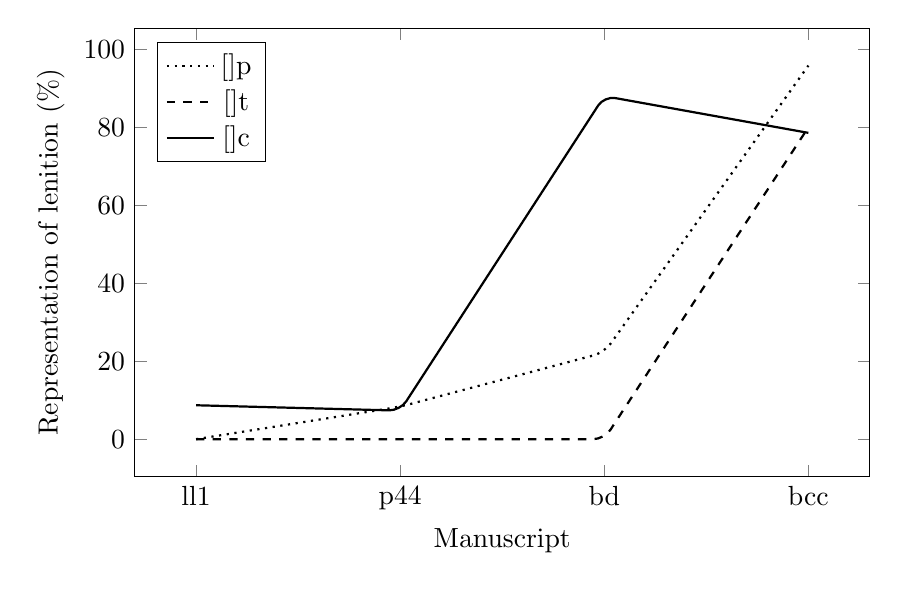
\begin{tikzpicture}
    \begin{axis}[
      width=.9\linewidth,
      height=.6\linewidth,
      xlabel=Manuscript,
      ylabel={Representation of lenition (\%)},
      symbolic x coords={
        \gls{ll1},
        \gls{p44},
        \gls{bd},
        \gls{bcc}
      },
      xtick=data,
      legend style={legend pos=north west},
      ]
      \addplot[color=black,rounded corners,thick,dotted,] coordinates {
        (\gls{ll1},0.00)
        (\gls{p44},8.33)
        (\gls{bd},22.22)
        (\gls{bcc},95.83)
      };
      \addplot[color=black,rounded corners,thick,dashed,] coordinates {
        (\gls{ll1},0.00)
        (\gls{p44},0.00)
        (\gls{bd},0.00)
        (\gls{bcc},80.00)
      };
      \addplot[color=black,rounded corners,thick] coordinates {
        (\gls{ll1},8.70)
        (\gls{p44},7.32)
        (\gls{bd},88.00)
        (\gls{bcc},78.57)
      };
      \legend{\mw[]{p},\mw[]{t},\mw[]{c}}
    \end{axis}
  \end{tikzpicture}
  \caption{Orthographical representation of voiceless stops over time.}
  \label{fig:linechartbrut}
\end{figure}

\subsection{Lenition in \acrshort{ll1} and \acrshort{p44}}
\label{sec:lenit-acrsh-acrsh}


The rule is clear in \gls{ll1} and \gls{p44}: lenition of voiceless stops is not written.
Given this rule, exceptions, constituting instances of representation of lenited voiceless stops, need to be accounted for.
These exceptions are found in Table~\ref{tab:ltrepll1p44}.
As can be seen in this table, both the form and meaning of the words themselves and their reason for being lenited differs, so accounting for them must be done on a case-by-case basis, and a satisfying account may not always be found.

\begin{table}[h]
  \centering
  \begin{tabular}{lddwql}
    \toprule
    \tch{Source} & \tch{Page} & \tch{Line} & \tch{Word} & \tch{Translation} & \tch{Reason lenition} \\
    \midrule
    \acrshort{ll1} & 34 & 1 & gellweyr & jest & \mw{trwy} \\
    \acrshort{ll1} & 35 & 8 & gytdỽundep & agreement & \mw{o} \\
    \acrshort{ll1} & 36 & 4 & gof & memory & \mw{ar} \\
    \acrshort{ll1} & 37 & 17 & glaf & sick & \mw{en} \\
    \acrshort{p44} & 25 & 10 & gewylyd & shame & \mw{en} \\
    \acrshort{p44} & 26 & 2 & gynt & before & adv phrase \\
    \acrshort{p44} & 26 & 9 & bryt & moment & \mw{pa} \\
    \acrshort{p44} & 27 & 6 & glaf & sick & \mw{en} \\
    \bottomrule
  \end{tabular}%
  \caption{Instances of \lT\ represented in \acrshort{ll1} and \acrshort{p44}.}
  \label{tab:ltrepll1p44}
\end{table}

One word that may be accounted for, however, is \mw[before]{gynt} (\gls{p44} 26.2).
It stands out in that it is the only lenited adverbial phrase in this source.
Moreover, lenition of adverbial phrases of time is often petrified, \eg \gmow[yesterday]{ddoe}.
The writing of \mw{gynt} with \mw{g} may similarly point to \gls{petr}, rather than \gls{morphophonlen}.
If so, this word constitutes a research exception.

The case of \mw[what moment?]{pa bryt} may be explained in a similar manner.
Although lenition following \mw{pa} is morphophonemic and still grammatical, it occurs frequently in combination with \mw{bryt}, so orthographical lenition is reminiscent of the \gls{petr} we find in research exception \mw[together]{y gyt}.
Comparison with phrases  such as \gmob[when]{peur < pe eur} also shows that interrogative pronouns containing \mw{pa} may be considered single words for the purpose of lenition.
Also, the semantics of the phrase obviously have a temporal dimension similar to \mw{gynt}.
The phrase \mw{pa bryt} is also found with exceptional lenition in \gls{bd}, as can be seen in Table~\ref{tab:replenpbd}.

After accounting for these two examples, we are still left with six examples of orthographically represented \gls{morphophonlen}.
These examples are few and far between, but nevertheless essential, because they show that lenition of voiceless stops \emph{could} be represented.
This means that writing \graph{b, d, g} for \lT\ had already been invented by the mid-thirteenth century.
It had just not been adopted widely.


\subsection{Lenition in \acrshort{bd} }
\label{sec:lenition-acrshortbd-}
In \gls{bd}, the rule is that lenition is not represented for \mw{p, t}, and it is represented for \mw{c}.
This rule is exceptionless for \mw{t}, but not for \mw{p} and \mw{c}.
These exceptions constitute instances where lenition is represented for \mw{p}, and for \mw{c} these exceptions constitute instances where lenition is not represented.
Table~\ref{tab:replenpbd} shows the two instances of orthographically represented lenited \mw{p}, and Table~\ref{tab:nonlencbd} shows every instance where lenited \mw{c} is not orthographically represented.

\begin{table}[h]
  \centering
  \begin{tabular}{addwql}
    \toprule
    \tch{Source} & \tch{Page} & \tch{Line} & \tch{Word} & \tch{Translation} & \tch{Reason lenition} \\
    \midrule
    bd & 34 & 4 & bryt & moment & \mw{pa} \\
    bd & 36 & 2 & baraỽt & ready & \mw{yn} \\
    \bottomrule
  \end{tabular}
  \caption{Representation of lenited \mw{p} in \acrshort{bd}}
  \label{tab:replenpbd}
\end{table}

\begin{table}[h]
  \centering
  \begin{tabular}{addwql}
    \toprule
    \tch{Source} & \tch{Page} & \tch{Line} & \tch{Word} & \tch{Translation} & \tch{Reason lenition} \\
    \midrule
    bd & 29 & 10 & caerussalem & (place name) & fem noun \\
    bd & 30 & 14 & kyuoeth & kingdom & \mw{y} ‘his' \\
    bd & 31 & 8 & kyuoeth & kingdom & \mw{y} ‘his' \\
    bd & 31 & 9 & kyuoeth & kingdom & \mw{y} ‘his' \\
    bd & 33 & 2 & caffei & received & \mw{na} \\
    bd & 35 & 1 & keissyaỽ & seek & \mw{y} ‘to' \\
    \bottomrule
  \end{tabular}%
  \caption{Non-representation of lenited \mw{c} in \acrshort{bd}}
  \label{tab:nonlencbd}
\end{table}

\subsection{Lenition in \acrshort{bcc}}
\label{sec:lenition-acrshortbcc}


Lenition of voiceless stops is as a rule represented in \gls{bcc}, so instances where lenition is not shown are the ones that need to be accounted for.
Table~\ref{tab:ltnotrepbcc} shows these instances of non-represented lenition.
Various reasons for lenition appear multiple times in this table.



\begin{table}[h]
  \centering
  \begin{tabular}{lddwql}
    \toprule
    \tch{Source} & \tch{Page} & \tch{Line} & \tch{Word} & \tch{Translation} & \tch{Reason lenition} \\
    \midrule
    \gls{bcc} & 16r & 29 & prosessio & procession & \mw{y} ‘to' \\
    \gls{bcc} & 16v & 6 & keluydodeu & arts & prep adj \\
    \gls{bcc} & 17r & 14 & kereis & I loved & \mw{th} \\
    \gls{bcc} & 17r & 15 & caraf & I love & \mw{th} \\
    \gls{bcc} & 17r & 16 & kerir & is loved & \mw{th} \\
    \gls{bcc} & 17v & 18 & tywyssauc & prince & apposition \\
    \gls{bcc} & 17v & 29 & tywyssawc & prince & apposition \\
    \gls{bcc} & 18r & 12 & trugarhae & mercy & \mw{y} ‘his' \\
    \gls{bcc} & 18r & 25 & Cordeilla & (personal name) & \mw{-ei} \\
    \gls{bcc} & 19r & 10 & Cordeilla & (personal name) & \mw{-ei} \\
    \gls{bcc} & 19v & 4 & tywyssawc & prince & apposition \\
    \gls{bcc} & 19v & 4 & tywyssawc & prince & apposition \\
    \gls{bcc} & 19v & 5 & calet & hard & prep adj \\
    \gls{bcc} & 19v & 13 & cordeilla & (personal name) & \mw{y} ‘to' \\
    \gls{bcc} & 19v & 25 & creftwyr & craftsmen & prep adj \\
    \bottomrule
  \end{tabular}%
  \caption{Instances of \lT\ not represented in \acrshort{bcc}.}
  \label{tab:ltnotrepbcc}
\end{table}

Within \gls{bcc}, \mw[prince]{tywyssawc} is found four times in apposition to a personal name.
A lenitable noun in apposition to a personal name is found eight times within this source, and is lenited only once in \mw[prophet]{broffwid} (\gls{bcc} 16r.26).
Lenition of nouns in apposition is not shown for other types of consonants either, as the word \mw[king]{brenhin} is also found in unlenited form in this position.

The word \mw{prosessio} is a late, learned loanword from \glat[procession]{prōcessiō}.
Writing \glat{c} in this word with \mw{s} confirms a post-vernacular pronunciation.
Phonologically, the structure of the word does not look Middle Welsh, as /au/ had not yet turned into /o/ in the final syllable.
This means that \mw{prosessio} constitutes an instance of code switching, or a recent loan.
Recent and transparent loanwords are not typically mutated in \gls{mow}, nor are instances of code switching.

The personal name \mw{Cordeilla} is found unlenited where lenition is expected on three separate occasions.
The fact that we are dealing with a personal name here may be of influence, as \mw{llyr} is found unlenited following \mw[fort]{caer} twice.
Furthermore, personal names are as a rule not lenited in \gls{mow}.
These instances of \mw{llyr} and \mw{Cordeilla} may be early examples of this \gls{mow} rule.
Additionally, \mw{Cordeilla} is a foreign name for the Welsh, and it may thus not have been lenited similarly to \mw{prosessio}.

Infixed object pronoun \mw{'th} should cause lenition, but this is not found in \gls{bcc}.
Lenition is problematic diachronically, as this pronoun causes provection in \gls{mco} and \gls{mb}.
Arguably, provection following this pronoun is also found in \gow[as it brings you]{imalitiduch} where medial \ow{t} represents both the /θ/ of the object pronoun, and preverb \ow{di} > \ow{ti}.

Several words following a preposed adjective fail to show lenition, although these instances are outnumbered by preposed adjectives shown to cause lenition.
Lenition following preposed adjectives is a type of free lenition, because all adjectives cause lenition when used as a preposed adjective.
These same adjectives do not as a rule cause lenition when they are in their usual postnominal position.
Consequently, the correct application of lenition hinges on the morphosyntactic relationship between two elements in the same clause rather than by simply checking whether the immediately preceding morpheme should cause lenition.
This morphosyntactic relationship may not always be clear or consistent.
Preposed adjectives are more frequent in this text than in \gls{mw} in general, because it is a translation from Latin, which further increases the likelihood of inconsistencies in the application of preposed adjectives.
An example where lenition following a  preposed adjective is to be expected is Example~\ref{ex:wychyrcalet}:
\mwcc[ex:wychyrcalet]{\gls{bcc} 19v.3--6}{ac yn ev herbyn wynt y doeth Maglawn tywyssawc yr alban. a henwyn tywyssawc kernyw ac ev holl allu. ac ymlad yn \al{wychyr calet} ac wynt.}{And against them came Maglawn, prince of Scotland, and Henwyn, prince of Cornwall, and their whole capability, and they fought \al{violently hard} against them.}
What exactly is the grammatical relationship between \mw[violent]{wychyr} and \mw[hard]{caled}?
Is \mw{wychyr} a preposed adjective followed by lenition, and translating to the translation given, or does \mw{caled} modify \mw{wychyr}, and are we not to expect lenition here?
In the latter case, `very violently' would be a more suitable translation%
\footnote{The Latin original is of little help either, as it is much terser than the Welsh: \lat[When this was done, Leir took his daughter and the assembled army to Britain. He fought with his sons-in-law and beat them.]{Quo facto, duxit secum leir filiam et collectam multitudinem in Britanniam pugnauitque cum generis et triumpho potitus est.}~\autocite[42--43]{Geo_History09}}.
And does the meaning matter at all for lenition?
At any rate, non-lenition is consistent, as the \mw{Brut} found in \gls{bcc} has four different instances of \mw{wychyr calet}, and each of them keeps the radical: 19v.5, 25v.14, 47v.12, 51r.29.
\Textcite[31--32]{morgan_y_1952} argues that constructions of the type  \mw{yn} + adjective + adjective  may be considered dvandva compounds or as compounds where one adjective typically has an intensifying function.
In any case, the repetition of adjectives constitutes the creation of a compound adjective, and thus always cause lenition, but that southern dialects tend to keep the radical here.
If Morgan is right, the example of  \mw{wychyr calet} seems like an aberration in both cases, because the second element should be lenited irrespectively of its semantics.
In the end, non-lenition may be a purely southern dialectal feature.

Many exceptions to the representation of lenition in \gls{bcc} stem from the difficulties involved in translating a Latin text.
After accounting for these, lenition seems to have been applied with great regularity, and remaining exceptions seem no more numerous than what is found in a \gls{mow} text of similar length, barring only the most carefully copy-edited ones.
As such, \gls{bcc} demonstrates that lenition of voiceless stops was wholly represented by the mid-fourteenth century.

\section{Lenited \mw{g}}
\label{sec:lenited-mwg}
The only number in Table~\ref{tab:perlenbrut} or Table~\ref{tab:perlenbrutex} not referring to a voiceless stop and dipping below the fifty per cent mark is that of the representation of lenited \mw{g} in \gls{p44}.
This begs the question why \mw{g} in \gls{p44} --- and to a lesser
extent in \gls{ll1} --- is lenited so infrequently.  In \gls{ll1}
lenited \mw{g} is shown in 49 out of 68 instances; in \gls{p44} it
is written in  only 26 out of 72 instances.  The element causing lenition
does not seem to be relevant, \eg verbal particle \mw{a} regularly
causes lenition to \mw[did]{oruc}, but not to \mw[did]{gwnaeth}.

The phonology of the lenited word does seem to play a role: when
initial \mw{g} is not followed by \mw{w}, it disappears in 48 out of
52 of such instances. The remaining four comprise the following
instances: \mw[they rested]{gorffowyssassant} (\gls{ll1} 38.25),
\mw[rested]{gor/ffowyssỽs} (\gls{p44} 23.9--10), \mw[gain]{gorescyn}
(\gls{p44} 27.15), and \mw[glorious]{gogonedỽs} (\gls{p44}
28.23). These words all historically started with \mw{g\cw}, but  \mw{\cw}
preceding \mw{o} has disappeared by the end of the \gls{ow} period. However, such words
starting with \mw{go} do represent lenition elsewhere, such as in the
plentiful instances of \mw[did]{oruc}.

The remaining 88 instances are all words starting with \mw{(g)w}, of which 27 show lenition.
Table~\ref{tab:gwphon} shows that the phonological structure of these words plays an important role in dictating whether lenition is written.
If the \mw{w} following lenited \mw{g} is vocalic, lenition is usually shown.
An example of such a word showing lenition is \mw[husband]{wr} (\gls{ll1} 34.13).
Similarly, lenition is usually shown if the quality of the following \mw{\cw} is consonantal, if this consonant is in turn followed by a vowel, \eg \mw[wear]{wyscaỽ} (\gls{p44} 27.7).
However, if the \mw{g} is followed by consonantal \mw{\cw}, and then followed by yet another consonant, lenition is usually not written, \eg \mw[make]{gwneỽthỽr} (\gls{p44} 27.28).

\begin{table}[h]
  \centering
  \begin{tabular}{ldd}
    \toprule
    & \tch{\graph{w}} & \tch{\graph{gw}}\\
    \midrule
    /ɡ\cw{}\gls{C}/ & 3 & 48\\
    /ɡ\cw{}\gls{V}/ or /ɡu/ &24 &13\\
    \bottomrule
  \end{tabular}
  \caption{Lenition of \mw{gw} divided by phonological structure of the word.}
  \label{tab:gwphon}
\end{table}

Not representing lenited \mw{g} served a purpose: it served to distinguish consonantal \mw{w} from its syllabic counterpart if it followed \mw{g} and preceded a consonant.
Maintaining  radical \mw{g} in the face of lenition served to indicate that the following \mw{\cw} before another consonant was consonantal, so that no reader of a phrase like \mw[his wife]{ẏ gwreic} would ever be fooled into saying /i ur…/ before reading the rest of the phrase and having to correct himself to /i \cw raɪɡ/.

\section{Conclusion}
\label{sec:conclusion-brut}
Lenition of voiceless stops was generally not written in the early thirteenth century, but it was not unfamiliarity with the concept of using \graph{b, d, g} for historical \mw{p, t, c} that kept them from writing lenition as such.
After all, these letters were used for \gls{petr}, and in exceptional cases even for \gls{morphophonlen}.
In the late thirteenth century, lenited \mw{c} came to be written as \mw{g}, but a similar shift did not occur for \mw{p} and \mw{t}.
These  departures from the thirteenth-century norm give us one key insight: lenition could be represented by this period, it had just not become the norm yet.

The case of lenited \mw{g} shows how the question of whether and how to write lenition may interplay with seemingly unrelated conundrums. 
A scribe who wished to ensure that no consonantal \mw{\cw} was mistaken for a vocalic \mw{w} had to weigh this wish against his wish to write lenition.
The former wish took precedence for the scribes of \gls{ll1} and \gls{p44}, and their priorities make sense in an orthographical tradition where the writing of lenition was limited to only several consonants, and where ability to read out loud would have been held in high esteem.

So what was the conundrum for voiceless stops?
What wish had to be weighed against the wish to represent lenition of these consonants?
The obvious answer to this question is that \lT≠\xD.
If lenited voiceless stops had not yet merged with radical voiced stops word-initially, then confusing the two when speaking might have been just as embarassing as using a vocalic \mw{w} for a consonantal \mw{\cw}. 
According to this line of reasoning, the phonological distinction between \lT\ and \xD\ argued for in Part~\ref{part:phonology-phonetics} must have survived until the middle of the thirteenth century.

%\todo[inline,caption={gg}]{For General conclusion: this means that not showing \lT\ is evidence of a early composition; probably dating back to  the period when they had not yet merged with \xD. However, the \mw{Brut} also shows that not writing \xD\ = \lT\ was by {choice}, rather than {ability}. They were able to write \lT\ like \xD\ as early as the thirteenth century, but they had to weigh representation of lenition against  the correct pronunciation of \lT\ separate from \xD. Another scribe (\eg of the Book of Aneirin) may have had different priorities, and could represent lenition of \lT. Ergo, writing lenition of \lT\ is not by itself a marker of lateness, but not writing lenition of \lT\ is, by contrast, a marker of earliness.}
%%% Local Variables:
%%% coding: utf-8
%%% mode: latex
%%% TeX-master: "../main"
%%% End:


\begin{spacing}{1}
\backmatter
\printglossary
\printglossary[%
    type=lang,%
    style=mcolindex,%
    nonumberlist=true,%
    nogroupskip=true]
\printglossary[type=\acronymtype]
\printbibliography
\end{spacing}
%%% Local Variables:
%%% mode: latex
%%% TeX-master: "main"
%%% End:
